% Options for packages loaded elsewhere
\PassOptionsToPackage{unicode}{hyperref}
\PassOptionsToPackage{hyphens}{url}
\PassOptionsToPackage{dvipsnames,svgnames,x11names}{xcolor}
%
\documentclass[
  letterpaper,
  DIV=11,
  numbers=noendperiod]{scrreprt}

\usepackage{amsmath,amssymb}
\usepackage{iftex}
\ifPDFTeX
  \usepackage[T1]{fontenc}
  \usepackage[utf8]{inputenc}
  \usepackage{textcomp} % provide euro and other symbols
\else % if luatex or xetex
  \usepackage{unicode-math}
  \defaultfontfeatures{Scale=MatchLowercase}
  \defaultfontfeatures[\rmfamily]{Ligatures=TeX,Scale=1}
\fi
\usepackage{lmodern}
\ifPDFTeX\else  
    % xetex/luatex font selection
\fi
% Use upquote if available, for straight quotes in verbatim environments
\IfFileExists{upquote.sty}{\usepackage{upquote}}{}
\IfFileExists{microtype.sty}{% use microtype if available
  \usepackage[]{microtype}
  \UseMicrotypeSet[protrusion]{basicmath} % disable protrusion for tt fonts
}{}
\makeatletter
\@ifundefined{KOMAClassName}{% if non-KOMA class
  \IfFileExists{parskip.sty}{%
    \usepackage{parskip}
  }{% else
    \setlength{\parindent}{0pt}
    \setlength{\parskip}{6pt plus 2pt minus 1pt}}
}{% if KOMA class
  \KOMAoptions{parskip=half}}
\makeatother
\usepackage{xcolor}
\setlength{\emergencystretch}{3em} % prevent overfull lines
\setcounter{secnumdepth}{5}
% Make \paragraph and \subparagraph free-standing
\ifx\paragraph\undefined\else
  \let\oldparagraph\paragraph
  \renewcommand{\paragraph}[1]{\oldparagraph{#1}\mbox{}}
\fi
\ifx\subparagraph\undefined\else
  \let\oldsubparagraph\subparagraph
  \renewcommand{\subparagraph}[1]{\oldsubparagraph{#1}\mbox{}}
\fi

\usepackage{color}
\usepackage{fancyvrb}
\newcommand{\VerbBar}{|}
\newcommand{\VERB}{\Verb[commandchars=\\\{\}]}
\DefineVerbatimEnvironment{Highlighting}{Verbatim}{commandchars=\\\{\}}
% Add ',fontsize=\small' for more characters per line
\usepackage{framed}
\definecolor{shadecolor}{RGB}{241,243,245}
\newenvironment{Shaded}{\begin{snugshade}}{\end{snugshade}}
\newcommand{\AlertTok}[1]{\textcolor[rgb]{0.68,0.00,0.00}{#1}}
\newcommand{\AnnotationTok}[1]{\textcolor[rgb]{0.37,0.37,0.37}{#1}}
\newcommand{\AttributeTok}[1]{\textcolor[rgb]{0.40,0.45,0.13}{#1}}
\newcommand{\BaseNTok}[1]{\textcolor[rgb]{0.68,0.00,0.00}{#1}}
\newcommand{\BuiltInTok}[1]{\textcolor[rgb]{0.00,0.23,0.31}{#1}}
\newcommand{\CharTok}[1]{\textcolor[rgb]{0.13,0.47,0.30}{#1}}
\newcommand{\CommentTok}[1]{\textcolor[rgb]{0.37,0.37,0.37}{#1}}
\newcommand{\CommentVarTok}[1]{\textcolor[rgb]{0.37,0.37,0.37}{\textit{#1}}}
\newcommand{\ConstantTok}[1]{\textcolor[rgb]{0.56,0.35,0.01}{#1}}
\newcommand{\ControlFlowTok}[1]{\textcolor[rgb]{0.00,0.23,0.31}{#1}}
\newcommand{\DataTypeTok}[1]{\textcolor[rgb]{0.68,0.00,0.00}{#1}}
\newcommand{\DecValTok}[1]{\textcolor[rgb]{0.68,0.00,0.00}{#1}}
\newcommand{\DocumentationTok}[1]{\textcolor[rgb]{0.37,0.37,0.37}{\textit{#1}}}
\newcommand{\ErrorTok}[1]{\textcolor[rgb]{0.68,0.00,0.00}{#1}}
\newcommand{\ExtensionTok}[1]{\textcolor[rgb]{0.00,0.23,0.31}{#1}}
\newcommand{\FloatTok}[1]{\textcolor[rgb]{0.68,0.00,0.00}{#1}}
\newcommand{\FunctionTok}[1]{\textcolor[rgb]{0.28,0.35,0.67}{#1}}
\newcommand{\ImportTok}[1]{\textcolor[rgb]{0.00,0.46,0.62}{#1}}
\newcommand{\InformationTok}[1]{\textcolor[rgb]{0.37,0.37,0.37}{#1}}
\newcommand{\KeywordTok}[1]{\textcolor[rgb]{0.00,0.23,0.31}{#1}}
\newcommand{\NormalTok}[1]{\textcolor[rgb]{0.00,0.23,0.31}{#1}}
\newcommand{\OperatorTok}[1]{\textcolor[rgb]{0.37,0.37,0.37}{#1}}
\newcommand{\OtherTok}[1]{\textcolor[rgb]{0.00,0.23,0.31}{#1}}
\newcommand{\PreprocessorTok}[1]{\textcolor[rgb]{0.68,0.00,0.00}{#1}}
\newcommand{\RegionMarkerTok}[1]{\textcolor[rgb]{0.00,0.23,0.31}{#1}}
\newcommand{\SpecialCharTok}[1]{\textcolor[rgb]{0.37,0.37,0.37}{#1}}
\newcommand{\SpecialStringTok}[1]{\textcolor[rgb]{0.13,0.47,0.30}{#1}}
\newcommand{\StringTok}[1]{\textcolor[rgb]{0.13,0.47,0.30}{#1}}
\newcommand{\VariableTok}[1]{\textcolor[rgb]{0.07,0.07,0.07}{#1}}
\newcommand{\VerbatimStringTok}[1]{\textcolor[rgb]{0.13,0.47,0.30}{#1}}
\newcommand{\WarningTok}[1]{\textcolor[rgb]{0.37,0.37,0.37}{\textit{#1}}}

\providecommand{\tightlist}{%
  \setlength{\itemsep}{0pt}\setlength{\parskip}{0pt}}\usepackage{longtable,booktabs,array}
\usepackage{calc} % for calculating minipage widths
% Correct order of tables after \paragraph or \subparagraph
\usepackage{etoolbox}
\makeatletter
\patchcmd\longtable{\par}{\if@noskipsec\mbox{}\fi\par}{}{}
\makeatother
% Allow footnotes in longtable head/foot
\IfFileExists{footnotehyper.sty}{\usepackage{footnotehyper}}{\usepackage{footnote}}
\makesavenoteenv{longtable}
\usepackage{graphicx}
\makeatletter
\def\maxwidth{\ifdim\Gin@nat@width>\linewidth\linewidth\else\Gin@nat@width\fi}
\def\maxheight{\ifdim\Gin@nat@height>\textheight\textheight\else\Gin@nat@height\fi}
\makeatother
% Scale images if necessary, so that they will not overflow the page
% margins by default, and it is still possible to overwrite the defaults
% using explicit options in \includegraphics[width, height, ...]{}
\setkeys{Gin}{width=\maxwidth,height=\maxheight,keepaspectratio}
% Set default figure placement to htbp
\makeatletter
\def\fps@figure{htbp}
\makeatother

\KOMAoption{captions}{tableheading}
\makeatletter
\makeatother
\makeatletter
\@ifpackageloaded{bookmark}{}{\usepackage{bookmark}}
\makeatother
\makeatletter
\@ifpackageloaded{caption}{}{\usepackage{caption}}
\AtBeginDocument{%
\ifdefined\contentsname
  \renewcommand*\contentsname{Table of contents}
\else
  \newcommand\contentsname{Table of contents}
\fi
\ifdefined\listfigurename
  \renewcommand*\listfigurename{List of Figures}
\else
  \newcommand\listfigurename{List of Figures}
\fi
\ifdefined\listtablename
  \renewcommand*\listtablename{List of Tables}
\else
  \newcommand\listtablename{List of Tables}
\fi
\ifdefined\figurename
  \renewcommand*\figurename{Figure}
\else
  \newcommand\figurename{Figure}
\fi
\ifdefined\tablename
  \renewcommand*\tablename{Table}
\else
  \newcommand\tablename{Table}
\fi
}
\@ifpackageloaded{float}{}{\usepackage{float}}
\floatstyle{ruled}
\@ifundefined{c@chapter}{\newfloat{codelisting}{h}{lop}}{\newfloat{codelisting}{h}{lop}[chapter]}
\floatname{codelisting}{Listing}
\newcommand*\listoflistings{\listof{codelisting}{List of Listings}}
\makeatother
\makeatletter
\@ifpackageloaded{caption}{}{\usepackage{caption}}
\@ifpackageloaded{subcaption}{}{\usepackage{subcaption}}
\makeatother
\makeatletter
\@ifpackageloaded{tcolorbox}{}{\usepackage[skins,breakable]{tcolorbox}}
\makeatother
\makeatletter
\@ifundefined{shadecolor}{\definecolor{shadecolor}{rgb}{.97, .97, .97}}
\makeatother
\makeatletter
\makeatother
\makeatletter
\makeatother
\ifLuaTeX
  \usepackage{selnolig}  % disable illegal ligatures
\fi
\IfFileExists{bookmark.sty}{\usepackage{bookmark}}{\usepackage{hyperref}}
\IfFileExists{xurl.sty}{\usepackage{xurl}}{} % add URL line breaks if available
\urlstyle{same} % disable monospaced font for URLs
\hypersetup{
  pdftitle={Apuntes y ejercicios de geoestadística para forestales},
  pdfauthor={Aitor Ameztegui},
  colorlinks=true,
  linkcolor={blue},
  filecolor={Maroon},
  citecolor={Blue},
  urlcolor={Blue},
  pdfcreator={LaTeX via pandoc}}

\title{Apuntes y ejercicios de geoestadística para forestales}
\author{Aitor Ameztegui}
\date{Invalid Date}

\begin{document}
\maketitle
\ifdefined\Shaded\renewenvironment{Shaded}{\begin{tcolorbox}[enhanced, frame hidden, sharp corners, breakable, boxrule=0pt, borderline west={3pt}{0pt}{shadecolor}, interior hidden]}{\end{tcolorbox}}\fi

\renewcommand*\contentsname{Table of contents}
{
\hypersetup{linkcolor=}
\setcounter{tocdepth}{2}
\tableofcontents
}
\bookmarksetup{startatroot}

\hypertarget{presentaciuxf3n}{%
\chapter*{Presentación}\label{presentaciuxf3n}}
\addcontentsline{toc}{chapter}{Presentación}

\markboth{Presentación}{Presentación}

Bienvenidos a laos apuntes y tutoriales de la asignatura
``Geoestadística y Técnicas de Observación Global''. Esta asignatura se
incluye en la doble titulación del Grado en Ingeniería Forestal y Grado
en Conservación de la Naturaleza. Se trata de una asignatura en la que
se enseñan técnicas y métodos para el análisis estadístico, modelización
y predicción de procesos espaciales.

\hypertarget{quuxe9-es-la-geoestaduxedstica}{%
\section*{¿Qué es la
geoestadística?}\label{quuxe9-es-la-geoestaduxedstica}}
\addcontentsline{toc}{section}{¿Qué es la geoestadística?}

\markright{¿Qué es la geoestadística?}

La geoestadística es un tipo de estadística utilizada para analizar y
predecir los valores asociados a fenómenos espaciales o
espacio-temporales. Incorpora las coordenadas espaciales (y en algunos
casos temporales) de los datos en los análisis. Las primeras
herramientas geoestadísticas se desarrollaron para describir patrones
espaciales y interpolar valores en lugares donde no se tomaron muestras.
El análisis geoestadístico moderno permite también construir modelos de
interpolación e incertidumbre más precisos, incorporando análisis
mulivariados.

La geoestadística se utiliza ampliamente en muchos ámbitos de la ciencia
y la ingeniería, por ejemplo para estimar niveles de contaminantes y
determinar si constituyen una amenaza para la salud, para espacializar
los datos procedentes de muestreos no continuos, como el Inventario
Forestal Nacional , o para cartografiar características del suelo como
los nutrientes, salinidad, etc. Y relacionarlos con el rendimiento de
cultivos agrícolas o sistemas forestales, entre otros muchos:

En todos estos ejemplos el contexto general es que existe algún fenómeno
de interés que se produce en el paisaje y que se caracteriza a partir de
muestreos puntuales. La geoestadística se utiliza a continuación para
elaborar predicciones en las ubicaciones no muestreadas. En esta
asignatura se introducen los principios de la modelización estadística y
de la información espacial, para a continuación presentar las
herramientas disponibles para un análisis geoestadístico de los procesos
de interés.

\hypertarget{de-quuxe9-va-esta-asignatura-de-quuxe9-no-va}{%
\section*{¿De qué va esta asignatura? ¿De qué no
va?}\label{de-quuxe9-va-esta-asignatura-de-quuxe9-no-va}}
\addcontentsline{toc}{section}{¿De qué va esta asignatura? ¿De qué no
va?}

\markright{¿De qué va esta asignatura? ¿De qué no va?}

Esta asignatura se centra en \textbf{diferentes tipos de análisis
espacial}, y ofrece al alumno una primera aproximación a los diversos
tipos de análisis existentes, con una visión muy práctica. Sin embargo,
no se espera que el alumno aprenda tan sólo a realizar análisis
geoestadísticos, sino también a \textbf{interpretar los resultados}, y a
identificar qué tipo de análisis resultará más \textbf{adecuado} para
cada tipo de pregunta a resolver.

Si bien es importante definir cuál es el objetivo del curso, resulta
igualmente importante dejar claro \textbf{cuáles no son los objetivos
del mismo}, al menos no objetivos directos de la asignatura, para evitar
equívocos:

\begin{itemize}
\item
  \textbf{Estadística}: para realizar un análisis geoestadístico es
  evidente que se necesita \textbf{dominar algunos conceptos
  estadísticos}. Conceptos como \emph{muestra}, \emph{población},
  \emph{test de hipótesis} o \emph{significación} aparecerán de manera
  recurrente durante el curso. Sin embargo, no daremos por hecho un
  conocimiento profundo de los mismos, por lo que los explicaremos según
  las necesidades del alumnado. En cualquier caso, cabe destacar que
  esto no es un curso de estadística, por lo que los alumnos que
  identifiquen problemas en ese sentido deben referirse a sus apuntes de
  estadística de segundo curso. La excepción en este sentido es la
  \textbf{regresión lineal}, para la que se realizará un repaso en
  profundidad (Chapter~\ref{sec-RegLin}).
\item
  \textbf{Sistemas de información geográfica (GIS)}: evidentemente, un
  análisis geoespacial implica una ubicación de los fenómenos que
  estudiaremos. Es decir, nuestros datos tendrán \textbf{coordenadas}.
  Aunque la ubicación de los objetos es una característica fundamental
  en la geoestadística, no debe confundirse esta asignatura con un curso
  de SIG. Conceptos como archivo \emph{vectorial}, \emph{raster},
  \emph{sistema de referencia de coordenadas} (CRS), \emph{intersección
  de capas} etc. serán frecuentes a la hora de trabajar con los ficheros
  espaciales, pero se supone un conocimiento suficiente por parte del
  alumnado (un conocimiento básico de SIG es suficiente). Sin embargo,
  sí dedicaremos un tema al \textbf{manejo y visualización de
  información} espacial en R (Chapter~\ref{sec-SpatialData})
\item
  \textbf{Cartografía}: La cartografía es la rama de la geografía
  encargada de la \textbf{representación gráfica} de un área geográfica,
  usualmente en términos bidimensionales y convencionales. Es decir que
  la cartografía es el arte y la ciencia de hacer, analizar, estudiar y
  comprender todo tipo de mapas. Cualquiera puede hacer un mapa, pero un
  mapa que comunique al público destinatario de manera adecuada debe
  respetar los principios del \emph{diseño cartográfico} (por ejemplo,
  la legibilidad). Aunque en esta asignatura produciremos numerosos
  mapas, conocer los elementos cartográficos y las reglas de la
  elaboración cartográfica quedan fuera del alcance de la misma, si bien
  se repasaran algunas nociones (\emph{escala}, \emph{leyenda}\ldots)
\item
  \textbf{R y RStudio}: R como hemos comentado, esta es una asignatura
  eminentemente práctica, y \textbf{R es el software elegido} como
  herramienta principal para realizar la mayoría de los análisis
  espaciales. Hemos elegido R por numerosos motivos, que van desde su
  versatilidad (funciona en cualquier sistema operativo), su carácter
  abierto y gratuito, su potencia y capacidad de análisis, o su
  creciente popularidad en el ámbito profesional y académico. Los
  alumnos se familiarizarán con el uso de R como herramienta de
  análisis, utilizándolo además para presentar los informes de
  prácticas. Sin embargo, aunque esta asignatura no es un curso de R,
  incluye una \textbf{Unidad 0} que pretende ofrecer a los estudiantes
  una introducción tanto al lenguaje de programación R
  (Chapter~\ref{sec-introR}) como a las herramientas RStudio
  (Chapter~\ref{sec-RStudio}) y Quarto (Chapter~\ref{sec-Quarto}), que
  se utilizarán durante el curso. Esta Unidad 0 queda a disposición de
  los y las estudiantes para refrescar conceptos relativos a R y como
  fuente de consulta de dudas durante todo el curso. Además, pueden
  plantearse al profesorado cualquier duda relativa a las herramientas
  que usaremos.
\end{itemize}

\hypertarget{quuxe9-hay-de-especial-en-lo-espacial}{%
\section*{¿Qué hay de especial en lo
espacial?}\label{quuxe9-hay-de-especial-en-lo-espacial}}
\addcontentsline{toc}{section}{¿Qué hay de especial en lo espacial?}

\markright{¿Qué hay de especial en lo espacial?}

Los sistemas espaciales son \emph{especiales} debido a las relaciones
espaciales inherentes y a las características temporales de las
entidades geográficas. Por lo tanto, es necesario tener en cuenta el
contexto y las relaciones espaciotemporales a la hora de modelizar y
simular procesos espaciales.

En otras palabras, el análisis espacial tiene en cuenta \textbf{de
manera explícita} las relaciones espaciotemporales que existen entre los
objetos de estudio, y pretende extraer conclusiones derivadas no sólo de
sus valores, sino \textbf{también de su ubicación} espaciotemporal. Un
caso que se suele citar habitualmente como primer análisis espacial es
el mapa del cólera de John Snow (ver recuadro).

\begin{quote}
\textbf{El mapa del cólera de John Snow} A mediados del siglo XIX, la
creencia general presuponía que el cólera se propagaba a través del
aire. La teoría de los microbios y su relación con las enfermedades aún
no estaba establecida (Pasteur tardaría aún 10 años en realizar los
experimentos que le darían validez) y los brotes de cólera que asolaban
Londres hacia 1850 eran, para todos, un misterio. Snow fue un médico
inglés nacido en 1813, considerado el padre de la epidemiología. Al
contrario que otros compañeros, el pensaba que el cólera no se propagaba
por el aire, y sospechaba que lo hacía por el agua contaminada. Para
demostrarlo, en 1854 empezó a registrar los casos de cólera del barrio
del Soho, sobre un mapa que contenía la ubicación de las fuentes.
Representaba cada muerte como un punto rojo ubicado sobre el lugar de
residencia. En total, registró 578 muertes, y el resultado no dejaba
lugar a pocas dudas: casi todos los casos se concentraban alrededor de
la fuente de Broad Street. Sin embargo, también había casos aislados,
fuera del área de influencia de la fuente, excepciones que Snow
documentó de manera exhaustiva hasta descubrir el origen del caso.
Además de sus análisis geográficos, Snow tomó muestras de las distintas
fuentes y las analizó bajo el microscopio, confirmando la presencia de
un organismo desconocido en la fuente de Broad Street. Aunque aún no se
conocía el papel de los microbios en la transmisión de enfermedades, las
autoridades decidieron cerrar la fuente por precaución, y el brote de
cólera remitió inmediatamente. Finalmente, se descubrió que la fuente
había sido contaminada por un pañal arrojado a un pozo negro cercano.

\includegraphics{images/john_snow.png}
\end{quote}

Pero además, trabajar con datos espaciales requiere
\textbf{conocimientos especializados} y habilidades en áreas que son
específicas de la disciplina. Algunos ejemplos son:

\begin{itemize}
\item
  \textbf{Geodatos}: los datos geoespaciales están
  \emph{georreferenciados} a una ubicación sobre, debajo o encima de la
  superficie terrestre. Las mediciones de coordenadas pueden ser
  ambiguas y difíciles de manejar, ya que existen multitud de sistemas
  de coordenadas y datums geodésicos.
\item
  \textbf{Análisis espacial}: El componente de localización de los
  geodatos permite nuevos \emph{tipos de análisis} basados en la
  distribución espacial de una o varias capas de datos. Facilita el
  descubrimiento de tendencias, patrones y relaciones espaciales y
  resuelve problemas mediante el modelado espacial.
\item
  \textbf{Estadística espacial}: existe una potente colección de
  \emph{herramientas utilizadas para optimizar el muestreo} de datos
  espaciales; para interpolar datos puntuales (por ejemplo, Kriging),
  medir distribuciones (por ejemplo, análisis de puntos calientes o
  \emph{hotspots}), analizar patrones (por ejemplo, agrupación) y
  modelizar relaciones espaciales (por ejemplo, regresión ponderada
  geográficamente).
\end{itemize}

\hypertarget{cuuxe1ndo-un-anuxe1lisis-es-espacial}{%
\section*{¿Cuándo un análisis es
espacial?}\label{cuuxe1ndo-un-anuxe1lisis-es-espacial}}
\addcontentsline{toc}{section}{¿Cuándo un análisis es espacial?}

\markright{¿Cuándo un análisis es espacial?}

Hasta ahora hemos hablado de que la geoestadística es la disciplina que
trabaja con \emph{datos espaciales}, y hemos definido las
particularidades de trabajar con este tipo de datos. Pero ¿qué hace que
un dato sea espacial, o \emph{geodato}? La particularidad de los datos
geoespaciales, espaciales o geodatos (podemos considerar los tres
términos sinónimos) es que poseen dos tipos de información:

\begin{itemize}
\tightlist
\item
  El valor de la variable de interés, que llamaremos \emph{atributo}
\item
  La \emph{localización} de la observación
\end{itemize}

A diferencia de los geodatos, en los datos no espaciales la localización
no importa. Un ejemplo claro de datos espaciales o geodatos sería una
serie de valores de temperatura de un conjunto de estaciones
meteorológicas: tendremos el \emph{dato de la temperatura media} del
día, o la precipitación, pero \emph{también las coordenadas} de la
ubicación de la estación. Para predecir la temperatura que hará en un
punto concreto del territorio en el que no existe estación,
necesitaremos tener en cuenta ambos tipos de información: la temperatura
de las estaciones más cercanas, y su distancia al punto de interés. Este
procedimiento, que se llama interpolación espacial, es el que emplean
herramientas como los Atlas climáticos o las Apps meteorológicas como
Meteoblue o Accuweather.

\begin{figure}

{\centering \includegraphics{images/cover.png}

}

\caption{La predicción de datos meteorológicos mediante interpolación es
un claro ejemplo de análisis espacial}

\end{figure}

Lógicamente, también podríamos realizar algún tipo de análisis que no
utilice la información espacial. Por ejemplo, si calculamos simplemente
la media y la desviación típica de la temperatura máxima de todas las
estaciones de una provincia, no estaremos usando la ubicación de las
estaciones. En este caso, a pesar de la naturaleza espacial de los
datos, nuestro análisis no sería un análisis geoestadístico.

\hypertarget{tipos-de-preguntas-que-requieren-anuxe1lisis-espacial}{%
\section*{Tipos de preguntas que requieren análisis
espacial}\label{tipos-de-preguntas-que-requieren-anuxe1lisis-espacial}}
\addcontentsline{toc}{section}{Tipos de preguntas que requieren análisis
espacial}

\markright{Tipos de preguntas que requieren análisis espacial}

Como hemos comentado, las características propias de los datos
espaciales permite abordar preguntas diferentes - o complementarias - a
las que podríamos hacernos si no tenemos en cuenta la ubicación de los
datos. Estas preguntas pueden ser de muy diverso tipo, y en algunos
casos han dado lugar a subdisciplinas enteras dentro del análisis
espacial.

\begin{itemize}
\tightlist
\item
  Un primer tipo de preguntas busca conocer \textbf{dónde se producen
  los eventos}. En este caso, el valor de la variable (atributo) no es
  tan importante como su ubicación. Ejemplos de este tipo de preguntas
  serían: ¿la regeneración del pino albar se produce de manera dispersa
  o agrupada? ¿Existen zonas con mayor densidad de igniciones que otras?
  ¿Se localizan los robos de manera aleatoria o existen patrones de
  agrupación? También podemos analizar si las observaciones de un tipo
  (por ejemplo, de una especie) afectan a la probabilidad de observar
  otro tipo (otra especie), lo que nos da idea de posibles
  interacciones, tanto positivas como negativas, entre ellas. Este tipo
  de cuestiones son propias del análisis de patrones de puntos, o
  análisis de agregación, que trataremos en el tema
  Chapter~\ref{sec-PointPattern}.
\item
  Otro tipo de preguntas pretende \textbf{predecir el valor} de una
  variable en un punto del espacio en el que no la hemos medido. Por
  ejemplo, teniendo valores de temperatura de varias estaciones
  meteorológicas cercanas, ¿cuál es el valor de temperatura en nuestro
  rodal? Otro ejemplo sería determinar la altura media del arbolado que
  podemos esperar en un rodal en el que hemos medido tan sólo 5
  parcelas. Este tipo de preguntas pueden resolverse mediante
  interpolación espacial, que pretende predecir el valor a partir de los
  valores más cercanos al punto de interés
  (Chapter~\ref{sec-Interpolation}) o a partir de la regresión espacial,
  que utiliza una segunda variable auxiliar - y su ubicación - para
  realizar predicciones (Chapter~\ref{sec-SpatReg}).
\item
  Un último tipo de cuestiones que citaremos es el que pretende
  \textbf{identificar} si las observaciones geográficamente
  \textbf{cercanas} \textbf{son más similares} entre sí que las
  distantes. Esto, por ejemplo, nos permitiría detectar si existen
  ``\emph{hotspots}'' o zonas con mayor acumulación de biomasa que
  otras, o si existen zonas en el monte donde se acumulen los rodales
  con mayor incidencia de plagas. Este tipo de cuestiones responden a
  análisis de autocorrelación espacial, y se tratarán en el tema
  Chapter~\ref{sec-Autocorrelacion}.
\end{itemize}

\hypertarget{funcionamiento-de-la-asignatura}{%
\section*{Funcionamiento de la
asignatura}\label{funcionamiento-de-la-asignatura}}
\addcontentsline{toc}{section}{Funcionamiento de la asignatura}

\markright{Funcionamiento de la asignatura}

\hypertarget{tipos-de-sesiones}{%
\subsection*{Tipos de sesiones}\label{tipos-de-sesiones}}
\addcontentsline{toc}{subsection}{Tipos de sesiones}

La asignatura se desarrollará en una serie de sesiones teóricas y
prácticas, que en ocasiones se combinarán durante una misma clase. Por
ello, todas las clases se llevarán a cabo en aula de informática.

\begin{itemize}
\item
  \textbf{Teoría}: introduciremos los principales conceptos teóricos
  necesarios para entender los temas y saber qué estamos haciendo cuando
  apliquemos las técnicas de análisis.
\item
  \textbf{Labs o tutoriales}: son sesiones guiadas de carácter práctico
  en el que aplicaremos los conceptos de la teoría a conjuntos de datos
  reales, produciendo un análisis de datos que interpretaremos
\item
  \textbf{Prácticas}: resolución de casos de estudio práctico en el que
  se aplicará lo visto en los dos tipos de sesiones anteriores. Se debe
  entregar un informe individual de cada práctica, que será evaluado.
\item
  \textbf{Exámenes}: se llevarán a cabo dos exámenes parciales. Se
  evaluará el conocimiento adquirido tanto durante las sesiones teóricas
  como en los labs.
\end{itemize}

\hypertarget{nuestras-herramientas}{%
\subsection*{Nuestras herramientas}\label{nuestras-herramientas}}
\addcontentsline{toc}{subsection}{Nuestras herramientas}

\hypertarget{r}{%
\subsubsection*{R}\label{r}}
\addcontentsline{toc}{subsubsection}{R}

El lenguaje de programación \texttt{R} se está convirtiendo en
\emph{lingua franca} en ciencia de datos, debido a sus capacidades y
versatilidad. \texttt{R} es un software
\href{https://cran.r-project.org/bin/windows/base/}{libre y gratuito},
que funciona en cualquier plataforma (Windows, Mac y Linux) y que tiene
numerosas funcionalidades. Entre ellas, además de servir como verdadero
lenguaje de programación, existe todo un conjunto de funcionalidades
espaciales avanzadas, disponibles en varias librerías que iremos
presentando en cada tema. Además de sus capacidades, una de las ventajas
de trabajar con código en vez de con programas de comandos y menús es la
posibilidad de guardar un script con todas las instrucciones ejecutadas,
de manera que los análisis en R son transparentes, compartibles, y
reproducibles. Esto es una gran ventaja a la que conviene acostumbrarse
lo más pronto posible, aunque al principio parezca poco eficiente, las
ganancias a medio/largo plazo son innumerables.

Sin embargo, R no es un SIG, y veremos que para algunos análisis, así
como para producir figuras y mapas de calidad profesional, no llega al
nivel de algunos software de pago como ArcGIS.

\hypertarget{rstudio}{%
\subsubsection*{RStudio}\label{rstudio}}
\addcontentsline{toc}{subsubsection}{RStudio}

Si R es la herramienta, el motor de los análisis que realizaremos,
RStudio es la consola de mandos. RStudio es un
\href{https://posit.co/downloads/}{entorno de desarrollo integrado}
(IDE) desarrollado por la compañía Posit (antes RStudio), que ofrece una
interfaz mucho más amigable de R. Además, tiene multitud de herramientas
útiles: autocompletado de comandos, gestión y visualización de archivos,
exportado de figuras, tablas; gestión de scripts (proyectos de RStudio).
utilizar R con RStudio no es obligatorio ni mucho menos, pero sí es muy
recomendable, ya que hace mucho más fácil usar R.

Además, RStudio tiene numerosos tutoriales, ayudas, videos\ldots{} que
nos ayudan en el proceso de aprendizaje de R.

\hypertarget{arcgis-pro}{%
\subsubsection*{ArcGis Pro}\label{arcgis-pro}}
\addcontentsline{toc}{subsubsection}{ArcGis Pro}

En anteriores ediciones de esta asignatura se ha utilizado, además de R,
ArcMap, el programa de GIS propiedad de ESRI. ArcMap ofrecía una serie
de funciones de análisis espacial muy avanzadas, con la ventaja de
ofrecer una interfz mucho más amable que R. Además, ArcMap ha sido
durante años el software con el que se ha enseñado SIG en la Universitat
de Lleida.

Desde julio de 2024, ESRI ha dejado de dar soporte de ArcMap, apostando
por la nueva herramienta de la compañía,
\href{https://www.esri.com/es-es/arcgis/products/arcgis-pro/overview?srsltid=AfmBOor-rlh2GqLGzdx_LmCzPqYP35N82fiTDYQXOsSUXbkYXSPNvmm7}{ArcGIS
Pro}. Por ello, desde el curso 24/25 la UdL no dispone de licencia
campus de ArcMap, si bien se pueden solicitar licencias individuales de
ArcGIS Pro. Por su versatilidad y su posición dominante en la industria
- sobre todo en algunos sectores - he considerado interesante ofrecer el
flujo de análisis de varios procesos en ArcGIS Pro.

\hypertarget{qgis}{%
\subsubsection*{QGis}\label{qgis}}
\addcontentsline{toc}{subsubsection}{QGis}

La alternativa más sólida y fiable a ArcGIS es actualmente
\href{https://www.qgis.org/}{QGIS}. Se trata de un software libre y
gratuito, que ofrece una serie de prestaciones realmente potente, en
ocasiones incluso superior a la que ofrecen los productos de ESRI. Para
el análisis geoestadístico existen un conjunto de plugins que se pueden
cargar a la instalación por defecto, entre las que destaca
\href{https://plugins.qgis.org/plugins/spatialanalysistoolbox/}{Spatial
Analysis Toolbox}. Sin embargo, a fecha de publicación de este libro, la
instalación del plugin presentaba problemas. Aún así, reproduciremos los
análisis en QGis cuando esto sea posible.

\hypertarget{evaluaciuxf3n}{%
\subsection*{Evaluación}\label{evaluaciuxf3n}}
\addcontentsline{toc}{subsection}{Evaluación}

El sistema de evaluación de la asignatura será mediante evaluación
continua, de acuerdo a la normativa de la Universitat de Lleida.
Existirán tres bloques, cada uno de ellos recuperable (ver más abajo):

\begin{longtable}[]{@{}lll@{}}
\toprule\noalign{}
Bloque & Número de pruebas & Peso \\
\midrule\noalign{}
\endhead
\bottomrule\noalign{}
\endlastfoot
Primer parcial & 1 & 25\% \\
Segundo parcial & 1 & 25\% \\
Prácticas & 6 & 50\% \\
\end{longtable}

La asignatura se evaluará según la siguiente ponderación:~Ex. Parcial 1
x 0.25 + Ex. Parcial 2 x 0.25 + Prácticas x 0.5

Para aprobar la asignatura se debe obtener una nota igual o superior a
5.0, y cumplir las siguientes condiciones:

\begin{itemize}
\item
  \textbf{BLOQUE TEÓRICO:} para aprobar este bloque se debe obtener una
  nota ≥ 4,0 en cada uno de los parciales, independientemente de la nota
  de prácticas. Es decir, no se hará media con las prácticas a no ser
  que se cumpla el requisito mínimo anterior.~
\item
  \textbf{BLOQUE PRÁCTICO}: La nota mínima para superar la parte
  práctica es 5,0. La parte práctica consiste en la entrega de 6
  informes de prácticas. Para aprobar el bloque se debe obtenir una nota
  ≥ 5,0 en al menos 4 de las prácticas.~
\end{itemize}

\begin{quote}
\textbf{NOTA}: Cada~práctica~tendrá una \textbf{fecha de entrega
específica}. El retraso en la entrega de los informes se penalizará des
de un \textbf{-30\%} hasta un \textbf{-100\%} de la nota de la práctica
entregada fuera de plazo.
\end{quote}

\hypertarget{recuperaciuxf3n}{%
\subsubsection*{\texorpdfstring{\textbf{Recuperación}}{Recuperación}}\label{recuperaciuxf3n}}
\addcontentsline{toc}{subsubsection}{\textbf{Recuperación}}

En caso de que no se supere la nota mínima en alguno de los bloques
(teoría 1, teoría 2, prácticas), se podrán recuperar dentro del período
marcado por el centro (ETSEAFIV). En el caso de recuperación, la nota
máxima del bloque de prácticas no podrá ser superior a 5.

\hypertarget{plagio-o-copia}{%
\subsubsection*{\texorpdfstring{\textbf{Plagio o
copia}}{Plagio o copia}}\label{plagio-o-copia}}
\addcontentsline{toc}{subsubsection}{\textbf{Plagio o copia}}

La Ley 2/2022 de convivencia universitaria regula lo que se considera
fraude académico: cualquier comportamiento premeditado tendente a
falsear los resultados de un examen, propio o ajeno, realizado como
requisito para superar una asignatura o acreditar el rendimiento
académico. Las faltas pueden ser graves o muy graves. Puede consultar en
la web de la UdL
\href{https://www.udl.cat/export/sites/universitat-lleida/ca/udl/norma/.galleries/docs/Organitzacio_interna/Acord-19-2023-CG-28.2.2023-Normativa-de-Convivencia-Universitaria-UdL.pdf}{la
Normativa de convivencia universitaria.}

Si se copia o plagia con medios fraudulentos se retirará la actividad de
evaluación (por tanto quedará suspendida) y se hará llegar un informe y
las evidencias a la coordinación del máster ya los jefes de estudio para
iniciar un expediente disciplinario. Las sanciones aplicables incluyen,
entre otros y dependiendo de la gravedad de la falta, la pérdida del
derecho a ser evaluado de la asignatura, la pérdida de la matrícula de
un semestre o curso o la expulsión hasta tres años.

El plagio es especialmente fácil de ejecutarse cuando se trabaja con
scripts de código, por lo que se será \textbf{especialmente severo} con
los casos que incumplan la normativa de fraude académico.

\hypertarget{bibliografuxeda}{%
\section*{Bibliografía}\label{bibliografuxeda}}
\addcontentsline{toc}{section}{Bibliografía}

\markright{Bibliografía}

\begin{itemize}
\item
  Baddeley, Turner (2015) Spatial Point Patterns: Methodology and
  Applications with R. Routledge.
\item
  Cayuela, De la Cruz (2022)
  \href{https://www.mundiprensa.com/catalogo/9788484768333/analisis-de-datos-ecologicos-en-r?utm_source=pocket_mylist}{Análisis
  de datos ecológicos en R}. Mundiprensa
\item
  Maestre, Escudeo, Bonet
  (2008)\href{https://dialnet.unirioja.es/servlet/libro?codigo=347765}{Introducción
  al análisis espacial de datos en ecología y ciencias ambientales}. U.
  Rey Juan Carlos.
\item
  Pebesma, EJ; Bivand R, Gómez-Rubio V. 2008 Applied Spatial Data
  Analysis with R.~
\item
  Spatial Data Science with R. 2020 Available
  at\href{https://rspatial.org}{~https://rspatial.org}
\end{itemize}

\part{UNIDAD 0: INTRODUCCION}

\hypertarget{sec-RStudio}{%
\chapter{Familiarizándose con R y RStudio}\label{sec-RStudio}}

\hypertarget{introducciuxf3n.-objetivo.}{%
\section{Introducción. Objetivo.}\label{introducciuxf3n.-objetivo.}}

El objetivo principal de este \emph{lab} es presentarte \texttt{R} y
\texttt{RStudio}, el software que utilizaremos a lo largo del curso para
recopilar datos, trabajarlos, visualizarlos y producir análisis
estadísticos que nos permitan llegar a conclusiones fundamentadas sobre
los problemas planteados.

Asumiremos que no tienes ninguna experiencia previa con R o RStudio, así
que en este \emph{lab} cubriremos lo más básico, empezando por la
instalación del software y los primeros pasos. Si ya sabes \emph{algo}
de R, puede que encuentres algunos de los temas bastante básicos, y eres
libre de saltar a donde quieras dentro del documento. Ten en cuenta, sin
embargo, que a veces daré algunos consejos y sugerencias que pueden ser
interesantes incluso si tienes experiencia con R.

\hypertarget{quuxe9-son-r-y-rstudio}{%
\section{¿Qué son R y RStudio?}\label{quuxe9-son-r-y-rstudio}}

En este lab, y durante todo el curso, vamos a utilizar R a través de
RStudio. Esto no es obligatorio, por supuesto, pero es muy recomendable.
Es común al principio confundir los dos. \texttt{R} es un lenguaje de
programación, mientras que \texttt{RStudio} es un entorno de desarrollo
integrado (IDE), es decir, una interfaz que añade muchas herramientas y
características convenientes y hace mucho más fácil la experiencia de
usar \texttt{R}. Tomaré aquí la analogía de
\href{https://moderndive.com/index.html}{ModernDive} y la simplificaré
diciendo que, si \texttt{R} es el motor de un coche, \texttt{RStudio}
sería el panel de mandos. Y como ocurre con el coche, claro que podemos
ejecutar R sin RStudio, pero es mucho más fácil aprovechar sus múltiples
e interesantes características. Además, RStudio (y el propio R) es
gratuito, de código abierto y multiplataforma.

\includegraphics{images/01-intro-r/r_vs_rstudio_1.png}

\begin{quote}
\textbf{Instalación de R y RStudio} Recuerda que R es el nombre del
propio lenguaje de programación y RStudio es un IDE (es decir, una
interfaz), por lo que no podrás utilizar RStudio sin instalar
previamente R. \href{https://www.r-project.org/}{Descarga e instala la
última versión de R aquí}
\href{https://posit.co/download/rstudio-desktop/\#download}{Descarga e
instala RStudio aquí} Ten en cuenta que si utilizas los ordenadores de
la Universidad, estos ya tienen instaladas las versiones adecuadas de R
y RStudio.
\end{quote}

\hypertarget{la-interfaz-de-rstudio}{%
\section{La interfaz de RStudio}\label{la-interfaz-de-rstudio}}

La mala noticia es que R es un lenguaje de programación, y esto
significa que tienes que escribir comandos en \emph{código} R, y
ejecutarlos para obtener el resultado. No te preocupes, la buena noticia
es que no necesitas ser un programador experto para poder utilizar R y
sacar mucho partido a sus capacidades.

\hypertarget{apariencia-buxe1sica}{%
\subsection{Apariencia básica}\label{apariencia-buxe1sica}}

Cuando abras por primera vez RStudio serás recibido por tres paneles:

\begin{itemize}
\tightlist
\item
  La \emph{consola} interactiva de R (toda la izquierda)
\item
  Entorno/Historia (pestaña en la parte superior derecha) (si está en
  inglés, verás ``Environment/History''
\item
  Archivos/Plots/Paquetes/Ayuda/Visor (pestaña en la parte inferior
  derecha) (``Files/Plots/Packages/Help/Viewer'')
\end{itemize}

\begin{figure}

{\centering \includegraphics[width=8.53in,height=\textheight]{images/01-intro-r/01_rstudio.png}

}

\caption{Apariencia básica de RStudio al abrirlo}

\end{figure}

\hypertarget{consola}{%
\subsubsection{Consola}\label{consola}}

La consola es el corazón de R, es donde R realmente evalúa y ejecuta el
código. Esta consola en RStudio es lo único que obtendrías si decidieras
usar R sin RStudio. Lo primero que verás en la sesión interactiva de R
es un montón de información, seguida de un \texttt{\textgreater{}} y un
cursor parpadeante. Esto es un \emph{prompt} que indica que R está listo
para recibir nuevo código.

La consola opera con la idea de un bucle ``Leer, evaluar, imprimir'':
escribes comandos, R intenta ejecutarlos y luego devuelve un resultado.
Puedes escribir el código directamente en la consola después del
\emph{prompt} y obtener una respuesta inmediata, o copiarlo desde otro
lugar (un editor de texto, por ejemplo) y pegarlo en la consola. Por
ejemplo, si escribes \texttt{1\ +\ 1} en la consola y pulsas enter
(¡házlo ahora!), verás que R da inmediatamente una salida de \texttt{2}.
¡Eh, ya \emph{estás} usando R!

\hypertarget{environmenthistory}{%
\subsubsection{Env\textasciitilde ironment/History}\label{environmenthistory}}

La pestaña \textbf{Entorno} (Environment/History) muestra los nombres de
todos los objetos que has creado o cargado en tu sesión actual de R (no
te preocupes, lo veremos más adelante). También puedes ver información
como el número de observaciones y filas en los objetos. La pestaña
también tiene algunas acciones en las que se puede hacer clic como
\texttt{Import\ Dataset} que abrirá una interfaz gráfica de usuario
(GUI) para importar datos en R.

La pestaña \textbf{Historial} de este panel muestra un historial de todo
el código que has evaluado previamente en la Consola. Tal vez no se
utiliza tanto como la pestaña \textbf{Entorno}, pero puede ser muy útil
en momentos puntuales.

A medida que te sientas más cómodo con R, puede que encuentres el panel
\emph{Entorno / Historial} más y más útil. Pero al principio
probablemente lo ignorarás, así que puedes incluso minimizar la ventana
haciendo clic en el botón \emph{minimizar} en la parte superior derecha
del panel.

\hypertarget{files-plots-packages-help}{%
\subsubsection{Files / Plots / Packages /
Help}\label{files-plots-packages-help}}

El panel \textbf{Files / Plots / Packages / Help} muestra mucha
información útil. Vamos a ver cada pestaña en detalle:

\begin{itemize}
\item
  \textbf{Archivos:} te da acceso al directorio de archivos de tu disco
  duro, por lo que es muy útil para encontrar y cargar scripts de
  código. Una buena característica del panel ``Archivos'' es que puedes
  usarlo para establecer tu directorio de trabajo: si tienes todos tus
  archivos en una carpeta (lo cual deberías), puedes apuntar a ella
  haciendo clic en ``Más'' y luego en ``Establecer como directorio de
  trabajo.'' Esto facilitará el proceso de leer y guardar archivos,
  porque RStudio apuntará a ese directorio por defecto. De esta manera
  no necesitarás indicar la ruta completa cuando quieras cargar un
  archivo a R.
\item
  \textbf{Plots:} este panel muestra todos los plots (figuras) que se
  generan durante una sesión de R. Hay botones para abrir el gráfico en
  una ventana separada y para exportar el gráfico como \texttt{.pdf} o
  \texttt{.jpeg}. Para ver cómo se muestran los gráficos en el panel
  \texttt{Plots}, simplemente copia el código siguiente en la
  \texttt{consola} para mostrar un histograma de la longitud de los
  pétalos de tres especies de plantas de Iris, que están incluidas en la
  base de datos \texttt{iris} (cargada con la instalación básica de R).
  Cuando lo hagas, deberías ver un histograma con la distribución del
  ancho de los pétalos para tres especies de Iris.
\end{itemize}

\begin{Shaded}
\begin{Highlighting}[]
\FunctionTok{hist}\NormalTok{(iris}\SpecialCharTok{$}\NormalTok{Petal.Width, }\AttributeTok{col =} \StringTok{"orange"}\NormalTok{, }\AttributeTok{main =} \StringTok{"Histogram of petal widths"}\NormalTok{)}
\end{Highlighting}
\end{Shaded}

\begin{figure}[H]

{\centering \includegraphics{00_Familiar_RStudio_files/figure-pdf/unnamed-chunk-1-1.pdf}

}

\end{figure}

\begin{itemize}
\item
  \textbf{Paquetes:} muestra una lista de todos los paquetes de R
  instalados en su disco duro e indica si están cargados o no. Los
  paquetes que están cargados en la sesión actual están marcados,
  mientras que los que están instalados pero no cargados todavía están
  desmarcados. Hablaremos de los paquetes más adelante.
\item
  \textbf{Ayuda:} menú de ayuda para las funciones de R. Podemos
  escribir el nombre de una función en la ventana de búsqueda, o
  utilizar el código para buscar una función con el nombre. También
  veremos qué son las funciones en un minuto.
\end{itemize}

Por supuesto, el diseño en RStudio puede ser modificado, y el usuario
puede configurar qué paneles ver, el color del código, y muchas otras
cuestiones. Puedes aprender más sobre la personalización de RStudio
\href{https://support.posit.co/hc/en-us/articles/200549016-Customizing-the-RStudio-IDE}{aquí}.
De todos modos, no te preocupes por los diferentes paneles y sus
funcionalidades por ahora. Aprenderás más sobre ellos a medida que los
usemos durante el curso, y espero que pronto te familiarices con ellos.

\hypertarget{conceptos-buxe1sicos-y-terminologuxeda}{%
\section{Conceptos básicos y
terminología}\label{conceptos-buxe1sicos-y-terminologuxeda}}

Antes de empezar a usar R, necesitamos definir algunos conceptos de
programación que saldrán a menudo. No es necesario que memorices ninguno
de estos conceptos, ya que te familiarizarás con ellos, pero si en algún
momento tienes dudas sobre lo que estamos hablando, puedes consultar
esta sección (o preguntarme a mí, por supuesto).

\begin{itemize}
\item
  \textbf{Código}: un trozo de texto que R entiende y es capaz de
  ejecutar
\item
  \textbf{Ejecutar código}: el acto de decirle a R que lea el código y
  realice las acciones que contenga. Para ejecutar un determinado trozo
  de código, lo escribimos en la consola y pulsamos Enter.
\item
  \textbf{Objetos}: siempre que guardamos algo en R, creamos un objeto.
  Una vez guardado, podemos realizar operaciones con los objetos,
  mostrar su contenido o reasignar su valor (ya veremos cómo). Los
  objetos pueden ser de muchos tipos, como veremos más adelante.
\item
  \textbf{Funciones} (a veces también llamadas comandos): un tipo
  específico de objeto, las funciones realizan tareas en R. Toman
  algunas entradas (llamadas \emph{argumentos}), y devuelven algunas
  salidas. Como ejemplo, la función \texttt{mean()} toma como argumento
  una cadena de valores numéricos - que deben introducirse entre
  paréntesis - y devuelve\ldots{} bueno, su media. Trabajaremos mucho
  con funciones a lo largo de este curso, y tendrás mucha práctica con
  ellas. Para ayudarte a entender cuándo estamos hablando de una
  función, también incluiré el \texttt{()} después de ellas, como
  hicimos con \texttt{mean()} más arriba.
\item
  \textbf{Paquetes}: algunas funciones están incluidas en la instalación
  estándar de R. Sin embargo, la comunidad de R es rica y muy activa, y
  cada día se crean cientos de paquetes. Un paquete no es más que una
  colección de funciones que ha sido creada y liberada para la comunidad
  (recuerda que R es un software de código abierto). Entre los paquetes
  que usaremos durante el curso están varios de los principales para
  tratar con datos espaciales: \texttt{tmaps}, \texttt{sf},
  \texttt{terra}\ldots)
\item
  \textbf{Scripts}: podemos escribir instrucciones (es decir, código)
  directamente en la consola, pero esta no es la forma más eficiente de
  trabajar. El 99\% de las veces deberías escribir tus comandos en un
  script. Un script no es más que un archivo de texto que contiene un
  conjunto ordenado de instrucciones. Esto significa que podemos
  escribir un archivo con las instrucciones que queremos ejecutar y
  luego ejecutarlas todas a la vez, o decidir qué parte ejecutar. Lo
  mejor de los scripts es que nos permite guardar el código para poder
  ejecutarlo más tarde, o seguir trabajando en él.
\end{itemize}

\hypertarget{quuxe9-son-los-paquetes-de-r}{%
\subsection{¿Qué son los paquetes de
R?}\label{quuxe9-son-los-paquetes-de-r}}

Como hemos visto, los paquetes de R amplían la funcionalidad de R
proporcionando funciones adicionales, y a menudo también incluyen datos
y documentación. Están escritos por una comunidad mundial de usuarios de
R y pueden descargarse gratuitamente de Internet. Existe un repositorio
``oficial'' de paquetes R llamado
\href{https://cran.r-project.org/web/packages/index.html}{CRAN}
(Comprehensive R Archive Network), pero los usuarios también pueden
alojar sus paquetes en cualquier repositorio de software (por ejemplo,
este es un enlace a mi paquete
\href{https://github.com/ameztegui/neighborhood}{neighborhood}, alojado
en mi sitio \href{https://github.com/ameztegui}{GitHub}).

Deberías pensar en los paquetes de R como en las aplicaciones que
descargas en tu teléfono móvil. Un teléfono nuevo tiene ciertamente
algunas características agradables cuando lo enciendes por primera vez,
pero una de las primeras cosas que hacemos es instalar nuestras
aplicaciones favoritas. Así que vamos a ver lo que tenemos que hacer
para instalar un paquete de R.

\hypertarget{instalaciuxf3n-de-paquetes}{%
\subsubsection{Instalación de
paquetes}\label{instalaciuxf3n-de-paquetes}}

Cada vez que se instala una nueva versión de R (R está en continuo
desarrollo, y las principales actualizaciones se producen cada 1-2 años)
hay que instalar de nuevo los paquetes deseados. Esto es lo mismo que
instalar WhatsApp desde Google Play o la App Store. En R hay dos formas
de instalar paquetes.

La forma más fácil es utilizar la pestaña ``Paquetes'' en RStudio. Allí,
puedes hacer clic en ``Instalar'', escribir el nombre del paquete que
quieres, y hacer clic en ``Instalar''. Y ¡voilà! El paquete está
instalado.

\includegraphics{images/01-intro-r/package_install.PNG}

Una segunda forma de instalar un paquete es simplemente escribir
\texttt{install.packages("el\_nombre\_del\_paquete")} en la Consola y
ejecutar este código (pulsando enter). Ten en cuenta que debe incluir
las comillas alrededor del nombre del paquete. Por ejemplo, ejecutar el
siguiente código instala el paquete \texttt{ggplot2}:

\begin{Shaded}
\begin{Highlighting}[]
\FunctionTok{install.packages}\NormalTok{(}\StringTok{"ggplot2"}\NormalTok{)}
\end{Highlighting}
\end{Shaded}

\hypertarget{cargando-paquetes}{%
\subsubsection{Cargando paquetes}\label{cargando-paquetes}}

Una vez que instales un paquete, no necesitarás instalarlo de nuevo, a
menos que actualices tu versión de R (siguiendo con la metáfora, esto
sería como comprar un nuevo móvil), o quieras actualizar el propio
paquete a una nueva versión. Sin embargo, al igual que hay que abrir la
aplicación de Instagram o WhatsApp antes de usarla, hay que cargar el
paquete antes de usar cualquiera de sus funciones. Esto se hace
escribiendo \texttt{library()}. Por ejemplo, prueba a escribir y
ejecutar \texttt{library(ggplot2)}.

Si después de ejecutar el código anterior, aparece un cursor parpadeante
junto al signo \texttt{\textgreater{}} ``prompt'', significa que ha
tenido éxito y que el paquete \texttt{ggplot2} está cargado y listo para
ser utilizado. Si, por el contrario, obtiene un ``mensaje de error'' en
rojo que dice \texttt{...}

\begin{verbatim}
Error in library(ggplot2) : there is no package called ‘ggplot2’
\end{verbatim}

\ldots{} significa que no lo instalaste correctamente.

\hypertarget{uso-de-paquetes}{%
\subsubsection{Uso de paquetes}\label{uso-de-paquetes}}

Un error muy común que cometen los nuevos usuarios de R cuando quieren
usar paquetes es que se olvidan de ``cargarlos'' primero usando el
comando \texttt{library()} que acabamos de ver. Recuerda: \emph{tienes
que cargar cada paquete que quieras usar cada vez que inicies RStudio.}
Si no ``cargas'' primero un paquete, pero intentas usar una de sus
características, verás un mensaje de error similar a: Error: could not
find function

R te está diciendo que está tratando de usar una función en un paquete
que aún no ha sido ``cargado''. R no sabe dónde encontrar la función que
está utilizando. Casi todos los nuevos usuarios se olvidan de hacer esto
cuando empiezan, y es un poco molesto acostumbrarse a hacerlo. Sin
embargo, lo recordarás con la práctica y después de algún tiempo se
convertirá en algo natural para ti.

\hypertarget{salvando-nuestro-cuxf3digo-scripts-en-r}{%
\subsection{Salvando nuestro código: scripts en
R}\label{salvando-nuestro-cuxf3digo-scripts-en-r}}

Hemos visto que un script es un archivo que contiene código. El código
en el script no se ejecutará hasta que le digas explícitamente que se
ejecute. Esto significa que podemos escribir un archivo con las
instrucciones que queremos ejecutar y luego ejecutarlas a la vez, o
decidir qué parte ejecutar.La ventaja de esto es sencilla: si escribes
código en la consola, se ejecutará automáticamente, pero no se guardará.
Así, por ejemplo, si te equivocas al escribir el código en la consola,
tendrías que volver a escribirlo todo de nuevo. En cambio, si escribes
todo tu código en un script y luego lo guardas, estará disponible en
cualquier momento que lo necesites, y si necesitas volver a ejecutar
algunos análisis sólo tienes que abrir los scripts necesarios y ejecutar
todo el código que contienen. Trabajar en scripts bien organizados y
documentados que puedan ser reejecutados múltiples veces por cualquier
usuario es la base de la ciencia reproducible.

Podemos crear un nuevo script eligiendo la opción de menú
\texttt{Archivo\ /\ Nuevo\ archivo\ /\ R\ script}, o con el atajo de
teclado Ctrl + Alt + Mayúsculas + N. Una vez hecho esto, notaremos que
aparece un cuarto panel en RStudio. Podemos abrir varios scripts al
mismo tiempo, y se organizarán en pestañas. El nuevo script se llamará
\emph{Sin título 1}, y estará listo para que escribamos el código. Por
supuesto, podemos guardarlo donde queramos y con el nombre que deseemos.
Los archivos de script son archivos de texto, que pueden ser abiertos
por cualquier editor de texto, y compartidos con los colaboradores. Por
convención, los scripts de R tienen la extensión \texttt{.R}.

\begin{quote}
\textbf{Consejo:} Debes acostumbrarte lo más rápido posible a escribir
la mayor parte de tu código en un script. Escribe directamente en la
consola sólo para hacer análisis rápidos.
\end{quote}

\begin{figure}

{\centering \includegraphics{images/01-intro-r/scripts.PNG}

}

\caption{Una vista de la interfaz de RStudio inmediatamente después de
crear un script. Fíjate como el panel ``consola'' está ahora en la parte
de abajo, mientras que los scripts están en la parte superior.}

\end{figure}

Los comandos dentro de un script no se ejecutarán inmediatamente, sólo
cuando lo ordenes expresamente. Para ejecutar el comando en el que se
encuentra el cursor en ese momento es necesario pulsar
\texttt{Ctrl}+\texttt{Enter} o hacer clic en el comando \texttt{Run} en
la parte superior de las ventanas de script. Ten en cuenta que el cursor
no tiene que estar al principio del comando, y que el comando puede
extenderse por más de una línea, se ejecutará completamente.

Sin embargo, si una sola línea constituye un comando completo, R sólo
ejecutará un comando. Después de ejecutar un comando, el cursor saltará
automáticamente al siguiente comando, lo que hace que sea muy eficiente
ejecutar grandes trozos de código con sólo pulsar
\texttt{Ctrl}+\texttt{Enter} o hacer clic en \texttt{Run} varias veces.

\begin{figure}

{\centering \includegraphics{images/01-intro-r/new_script.gif}

}

\caption{El proceso completo de crear un nuevo script, esribir código, y
ejecutarlo. it.}

\end{figure}

Para controlar mejor el trozo de código que quieres ejecutar, puedes
seleccionarlo y pulsar \texttt{Ctrl}+\texttt{Enter}, y R ejecutará la
selección.

Para ejecutar todo el código del script, pulse \texttt{Ctrl+Mayús+Enter}
o haga clic en \texttt{Fuente} en la barra que hay encima del script.

\hypertarget{sec-introR}{%
\chapter{Introducción a R}\label{sec-introR}}

\hypertarget{introducciuxf3n.-objetivo.-1}{%
\section{Introducción. Objetivo.}\label{introducciuxf3n.-objetivo.-1}}

En el tutorial anterior vimos cómo instalar R y RStudio, así como alguna
de sus principales características. Una vez familiarizados con el
entorno en el que trabajaremos, es el momento de empezar a trabajar
\emph{realmente} con R. Como ya dijimos en la presentación de la
asignatura, R es una herramienta muy versátil, ya que podemos usarlo de
maneras muy distintas: puede ser desde una herramienta estadística hasta
un lenguaje de programación compleja. Vamos a ver a continuación algunos
de sus usos más básicos, y en el proceso iremos comentando algunas de
las particularidades de cómo funciona R. Como ya dijimos en el tutorial
anterior, si ya tienes experiencia usando R, puedes saltarte las partes
que ya domines.

\hypertarget{usando-r-como-una-calculadora}{%
\section{Usando R como una
calculadora}\label{usando-r-como-una-calculadora}}

Lo más sencillo que puedes hacer con R es utilizarlo como una
calculadora, es decir, para hacer aritmética. Por ejemplo, si escribimos
la siguiente expresión:

\begin{Shaded}
\begin{Highlighting}[]
\DecValTok{156} \SpecialCharTok{*} \DecValTok{35}
\end{Highlighting}
\end{Shaded}

\begin{verbatim}
[1] 5460
\end{verbatim}

Vemos que R imprimirá la respuesta, con un {[}1{]} precedente. No te
preocupes por esto por ahora, lo explicaremos más adelante. Por ahora
piensa en esto como una indicación de salida de resultados.

Si escribimos un comando incompleto, R esperará que lo completemos. Por
ejemplo, intenta escribir en la consola

\texttt{1\ +}

Cuando aprietes Return y la sesión de R muestre un \texttt{+} en vez de
\texttt{\textgreater{}}, quiere decir que está esperando a que
completemos el comando. Si queremos cancelar una orden incompleta
podemos clicar Escape y RStudio volverá a mostrar el icono
\texttt{\textgreater{}}. Esto también se puede usar para interrumpir un
proceso que se quede colgado o lleve demasiado tiempo.

Cuando se utiliza R como calculadora, el orden de las operaciones es el
mismo que aprendimos en el colegio. De mayor a menor precedencia:

\begin{itemize}
\tightlist
\item
  Paréntesis: \texttt{(}, \texttt{)}
\item
  Exponentes: \texttt{\^{}} or \texttt{**}
\item
  División: \texttt{/}
\item
  Multiplicación: \texttt{*}
\item
  Suma: \texttt{+}
\item
  Resta: \texttt{-}
\end{itemize}

Por ejemplo:

\begin{Shaded}
\begin{Highlighting}[]
\DecValTok{3} \SpecialCharTok{+} \DecValTok{2} \SpecialCharTok{*} \DecValTok{5}
\end{Highlighting}
\end{Shaded}

\begin{verbatim}
[1] 13
\end{verbatim}

\begin{Shaded}
\begin{Highlighting}[]
\NormalTok{(}\DecValTok{3} \SpecialCharTok{+} \DecValTok{2}\NormalTok{) }\SpecialCharTok{*} \DecValTok{5}
\end{Highlighting}
\end{Shaded}

\begin{verbatim}
[1] 25
\end{verbatim}

Los paréntesis pueden utilizarse para aclarar el sentido del código. Sin
embargo, puede resultar difícil de leer cuando hay muchos o cuando
realmente no es necesario. Recuerda que otros (¡o incluso tú mismo!)
pueden leer tu código más adelante, y es conveniente que sea lo más
inteligible posible.

\begin{Shaded}
\begin{Highlighting}[]
\DecValTok{3} \SpecialCharTok{+} \DecValTok{2} \SpecialCharTok{*} \DecValTok{5} \SpecialCharTok{\^{}} \DecValTok{2}       \CommentTok{\# claro, si recuerdas las reglas}
\end{Highlighting}
\end{Shaded}

\begin{verbatim}
[1] 53
\end{verbatim}

\begin{Shaded}
\begin{Highlighting}[]
\DecValTok{3} \SpecialCharTok{+} \DecValTok{2} \SpecialCharTok{*}\NormalTok{ (}\DecValTok{5} \SpecialCharTok{\^{}} \DecValTok{2}\NormalTok{)     }\CommentTok{\# probablemente más claro}
\end{Highlighting}
\end{Shaded}

\begin{verbatim}
[1] 53
\end{verbatim}

\begin{Shaded}
\begin{Highlighting}[]
\NormalTok{(}\DecValTok{3} \SpecialCharTok{+}\NormalTok{ (}\DecValTok{2} \SpecialCharTok{*}\NormalTok{ (}\DecValTok{5} \SpecialCharTok{\^{}} \DecValTok{2}\NormalTok{))) }\CommentTok{\# más difícil de leer}
\end{Highlighting}
\end{Shaded}

\begin{verbatim}
[1] 53
\end{verbatim}

Puede que hayas notado que parte del texto anterior no ha sido procesado
por R. En realidad, todo lo que sigue después del símbolo hash
\texttt{\#} es ignorado por R cuando ejecuta el código. El texto que
sigue a \texttt{\#} se llama ``comentario'', y puede ser muy útil para
recordar el propósito y los pasos de un determinado análisis.

\hypertarget{funciones-matemuxe1ticas}{%
\subsection{Funciones matemáticas}\label{funciones-matemuxe1ticas}}

R tiene muchas funciones matemáticas incorporadas. Para llamar a una
función, simplemente escribimos su nombre, seguido de los paréntesis de
apertura y cierre. Recuerda que todo lo que escribimos dentro de los
paréntesis se llama \emph{argumentos} de la función (los inputs que
requiere para funcionar).

\begin{Shaded}
\begin{Highlighting}[]
\CommentTok{\# Veamos algunas funciones trigonométricas}

\FunctionTok{sin}\NormalTok{(}\DecValTok{1}\NormalTok{)  }\CommentTok{\# seno de un número}
\end{Highlighting}
\end{Shaded}

\begin{verbatim}
[1] 0.841471
\end{verbatim}

\begin{Shaded}
\begin{Highlighting}[]
\FunctionTok{log}\NormalTok{(}\DecValTok{1}\NormalTok{)  }\CommentTok{\# logaritmo natural de un número}
\end{Highlighting}
\end{Shaded}

\begin{verbatim}
[1] 0
\end{verbatim}

\begin{Shaded}
\begin{Highlighting}[]
\FunctionTok{log10}\NormalTok{(}\DecValTok{10}\NormalTok{) }\CommentTok{\# logaritmo base 10}
\end{Highlighting}
\end{Shaded}

\begin{verbatim}
[1] 1
\end{verbatim}

\begin{Shaded}
\begin{Highlighting}[]
\FunctionTok{exp}\NormalTok{(}\FloatTok{0.5}\NormalTok{) }\CommentTok{\# e\^{}(1/2)}
\end{Highlighting}
\end{Shaded}

\begin{verbatim}
[1] 1.648721
\end{verbatim}

También podemos utilizar las funciones de R para calcular el máximo,
mínimo o media de una serie de valores, para obtener los elementos
distintos de una serie de elementos o para extraer elementos de una
cadena de caracteres.

\begin{Shaded}
\begin{Highlighting}[]
\FunctionTok{max}\NormalTok{(}\FunctionTok{c}\NormalTok{(}\DecValTok{1}\NormalTok{,}\DecValTok{2}\NormalTok{,}\DecValTok{5}\NormalTok{,}\DecValTok{6}\NormalTok{,}\DecValTok{7}\NormalTok{,}\DecValTok{9}\NormalTok{,}\DecValTok{12}\NormalTok{))}
\end{Highlighting}
\end{Shaded}

\begin{verbatim}
[1] 12
\end{verbatim}

\begin{Shaded}
\begin{Highlighting}[]
\FunctionTok{mean}\NormalTok{(}\DecValTok{1}\SpecialCharTok{:}\DecValTok{10}\NormalTok{)}
\end{Highlighting}
\end{Shaded}

\begin{verbatim}
[1] 5.5
\end{verbatim}

\begin{Shaded}
\begin{Highlighting}[]
\FunctionTok{unique}\NormalTok{(}\FunctionTok{c}\NormalTok{(}\DecValTok{3}\NormalTok{,}\DecValTok{3}\NormalTok{,}\DecValTok{4}\NormalTok{,}\DecValTok{5}\NormalTok{,}\DecValTok{6}\NormalTok{,}\DecValTok{6}\NormalTok{))}
\end{Highlighting}
\end{Shaded}

\begin{verbatim}
[1] 3 4 5 6
\end{verbatim}

\begin{Shaded}
\begin{Highlighting}[]
\FunctionTok{substr}\NormalTok{(}\StringTok{"abcdef"}\NormalTok{, }\DecValTok{2}\NormalTok{,}\DecValTok{4}\NormalTok{)}
\end{Highlighting}
\end{Shaded}

\begin{verbatim}
[1] "bcd"
\end{verbatim}

\begin{quote}
\textbf{Series de valores (vectores):} Has visto aquí arriba las dos
formas principales de crear vectores numéricos en R: concatenando
diferentes elementos dentro de la función \texttt{c()}, o definiendo un
intervalo mediante \texttt{1:10}, que equivaldría a decir
\texttt{de\ 1\ a\ 10}. Los vectores pueden contener valores numéricos o
caracteres, pero todos los elementos deben ser del mismo tipo. Veremos
más sobre vectores más adelante.
\end{quote}

\begin{quote}
\textbf{Recordando los nombres de las funciones y los argumentos:} Como
hemos dicho, R tiene multitud de funciones matemáticas, y muchas más
están incluidas en los paquetes. Una buena función tendrá un nombre
autoexplicativo que será fácil de recordar (por ejemplo,
\texttt{mean()}, \texttt{max()}\ldots). Sin embargo, no os preocupéis
por intentar recordar todas las funciones de R. Podéis simplemente
buscarlas en Google, o si recordáis el comienzo del nombre de la
función, escribidlo y pulsad la tecla Tab. Esto mostrará una lista de
funciones cuyo nombre coincide con lo que has escrito hasta ahora. Esto
se conoce como \texttt{completar\ con\ tabulador}, y puede ahorrar mucho
tiempo de escritura (y reducir el riesgo de errores de escritura). El
completado de tabulador funciona tanto en R como en RStudio. En RStudio
esta característica es aún más útil; un extracto del archivo de ayuda de
la función se mostrará junto al nombre de la función. Prueba a escribir
\texttt{me} y pulsa tab. Además, si pulsas Tab después de especificar el
nombre de la función y el paréntesis de apertura, RStudio proporciona
una lista de los argumentos que necesita esa función. Y si se pulsa Tab
cuando el cursor está entre dos comillas, proporcionará una lista con
las carpetas de tu directorio actual. Además, si escribes un \texttt{?}
antes del nombre de una función, se abrirá la página de ayuda de esa
función, que además de proporcionar una descripción detallada de la
función y de su funcionamiento, suele mostrar una colección de ejemplos
de código que ilustran el uso de la función. Al principio puede que no
encuentres estas características tan útiles, pero a medida que escribas
más código te encontrarás utilizándolas ampliamente.
\end{quote}

\hypertarget{comparando-objetos}{%
\subsection{Comparando objetos}\label{comparando-objetos}}

También podemos hacer comparaciones en R, y nos dirá si la comparación
que estamos probando es cierta (\texttt{TRUE}) o falsa (\texttt{FALSE}).
Por ejemplo, prueba las siguientes comparaciones:

\begin{Shaded}
\begin{Highlighting}[]
\DecValTok{1} \SpecialCharTok{==} \DecValTok{1}    \CommentTok{\# igualdad (se usan dos signos de igual, para diferenciarlo del \textasciigrave{}=\textasciigrave{} como asignación)}
\end{Highlighting}
\end{Shaded}

\begin{verbatim}
[1] TRUE
\end{verbatim}

\begin{Shaded}
\begin{Highlighting}[]
\DecValTok{1} \SpecialCharTok{!=} \DecValTok{2}    \CommentTok{\# desigualdad (se lee como "no es igual a")}
\end{Highlighting}
\end{Shaded}

\begin{verbatim}
[1] TRUE
\end{verbatim}

\begin{Shaded}
\begin{Highlighting}[]
\DecValTok{2} \SpecialCharTok{\textless{}} \DecValTok{1}     \CommentTok{\# menor que}
\end{Highlighting}
\end{Shaded}

\begin{verbatim}
[1] FALSE
\end{verbatim}

\begin{Shaded}
\begin{Highlighting}[]
\DecValTok{1} \SpecialCharTok{\textgreater{}} \DecValTok{0}     \CommentTok{\# mayor que}
\end{Highlighting}
\end{Shaded}

\begin{verbatim}
[1] TRUE
\end{verbatim}

\begin{Shaded}
\begin{Highlighting}[]
\DecValTok{6} \SpecialCharTok{\textless{}=} \DecValTok{6}    \CommentTok{\# menor o igual que}
\end{Highlighting}
\end{Shaded}

\begin{verbatim}
[1] TRUE
\end{verbatim}

\begin{Shaded}
\begin{Highlighting}[]
\DecValTok{1} \SpecialCharTok{\textgreater{}=} \SpecialCharTok{{-}}\DecValTok{9}   \CommentTok{\# mayor o igual que}
\end{Highlighting}
\end{Shaded}

\begin{verbatim}
[1] TRUE
\end{verbatim}

\hypertarget{objetos-en-r}{%
\section{Objetos en R}\label{objetos-en-r}}

Cada vez que almacenamos un determinado valor en la memoria de R,
estamos creando un \emph{objeto}. Esto es realmente importante, ya que
si no guardamos las operaciones, o los valores, como objetos, estos no
estarán disponibles más adelante. Es decir, R simplemente los imprimirá
en la consola pero no los almacenará en memoria. Vamos a crear un objeto
llamado \texttt{x}. Utilizamos \texttt{\textless{}-} para asignar
valores a un determinado objeto.

\begin{Shaded}
\begin{Highlighting}[]
\NormalTok{x }\OtherTok{\textless{}{-}} \DecValTok{3}
\end{Highlighting}
\end{Shaded}

\texttt{x} contiene ahora el valor \texttt{3}. Si buscamos la pestaña
\emph{Environment} en uno de los paneles de RStudio, veremos que han
aparecido \texttt{x} y su valor. Sin embargo, R no imprime nada cuando
hacemos esta asignación. En su lugar, lo almacena para más tarde en algo
llamado \emph{variable}, que es el tipo de objeto más simple en R. Las
variables se muestran en la pestaña \texttt{Environment} de RStudio, y
se almacenan en la memoria hasta que terminamos la sesión actual de R.
Para ver el valor almacenado en un objeto, simplemente pedimos a R que
evalúe \texttt{x} y nos muestra el valor almacenado:

\begin{Shaded}
\begin{Highlighting}[]
\NormalTok{x}
\end{Highlighting}
\end{Shaded}

\begin{verbatim}
[1] 3
\end{verbatim}

Una forma más explícita de pedirle a R que nos muestre el valor
almacenado en \texttt{x} es utilizando \texttt{print} de esta manera:

\begin{Shaded}
\begin{Highlighting}[]
\FunctionTok{print}\NormalTok{(x)}
\end{Highlighting}
\end{Shaded}

\begin{verbatim}
[1] 3
\end{verbatim}

Los objetos más sencillos en R son las variables como \texttt{x}, pero
en realidad, cualquier entidad que se cree y manipule en R puede ser
almacenada como objeto, incluyendo datos, funciones, modelos,
gráficos\ldots{} Para crear un objeto sólo tenemos que asignarle un
nombre. Ya hemos mencionado anteriormente que R es un lenguaje orientado
a objetos. Esto significa básicamente que está diseñado para utilizar
objetos como base de todas las tareas.

\begin{quote}
\textbf{Consejo: asignación} También es posible utilizar el operador
\texttt{=} para la asignación, como en: \texttt{x\ =\ 1/40}. Esto es
mucho menos común entre los usuarios de R, y más adelante veremos por
qué no es buena idea utilizarlo. Si lo usas, trata de cambiar tus
hábitos lo antes posible.
\end{quote}

\hypertarget{trabajando-con-variables}{%
\subsection{Trabajando con variables}\label{trabajando-con-variables}}

Lo interesante es que nuestra variable \texttt{x} está ahora almacenada
en memoria, por lo que puede utilizarse en lugar de un número en
cualquier cálculo que espere un número. Por ejemplo, prueba esto:

\begin{Shaded}
\begin{Highlighting}[]
\NormalTok{x }\SpecialCharTok{+} \DecValTok{3}
\end{Highlighting}
\end{Shaded}

\begin{verbatim}
[1] 6
\end{verbatim}

\begin{Shaded}
\begin{Highlighting}[]
\FunctionTok{log}\NormalTok{(x)}
\end{Highlighting}
\end{Shaded}

\begin{verbatim}
[1] 1.098612
\end{verbatim}

Las variables se pueden reasignar tantas veces como se desee, pero eso
significa que su valor anterior se borrará de la memoria:

\begin{Shaded}
\begin{Highlighting}[]
\NormalTok{x }\OtherTok{\textless{}{-}} \DecValTok{100}
\end{Highlighting}
\end{Shaded}

\texttt{x} solía contener el valor \texttt{3} y ahora tiene el valor
\texttt{100} (ver la pestaña \texttt{Environment} en RStudio).

Las asignaciones pueden contener la variable a la que se asigna, y en
este caso tomarán el valor almacenado actualmente, calcularán lo que
contenga el código y sobrescribirán el valor anterior con el nuevo.

\begin{Shaded}
\begin{Highlighting}[]
\NormalTok{x }\OtherTok{\textless{}{-}}\NormalTok{ x }\SpecialCharTok{*}\DecValTok{2} \CommentTok{\# observa cómo RStudio actualiza su descripción de x en la pestaña Environment}
\end{Highlighting}
\end{Shaded}

\begin{quote}
\textbf{Atención:} Aunque la posibilidad de sobreescribir una variable
como resultado de una operación es una de las características más útiles
de R, tiene su peligro. Al realizar tareas complejas, es
\textbf{extremadamente fácil} sobrescribir una variable sin querer, y
todos nuestros cálculos a partir de ese momento corren el riesgo de ser
erróneos. Por ejemplo, si ejecutas el código anterior dos veces en lugar
de una, \texttt{x} obtendrá un valor de \texttt{400} en lugar de
\texttt{200}. Si haces esto sin darte cuenta, \texttt{x} no tendrá el
valor que esperas que tenga. Además, si te equivocas en el código
anterior y R devuelve un mensaje de error, eso significa que no habrás
sobrescrito el valor de \texttt{x}, que seguirá siendo \texttt{100}. Por
lo tanto, \textbf{siempre} comprueba el valor actual de una variable (en
el panel ``Environment'') antes de realizar operaciones con ella.
\end{quote}

\hypertarget{tipos-de-datos}{%
\section{Tipos de datos}\label{tipos-de-datos}}

Las variables en R pueden ser de diferentes tipos. La función
\texttt{class} nos ayuda a determinar qué tipo de objeto tenemos:

\begin{Shaded}
\begin{Highlighting}[]
\NormalTok{x }\OtherTok{\textless{}{-}} \DecValTok{100}
\FunctionTok{class}\NormalTok{(x)}
\end{Highlighting}
\end{Shaded}

\begin{verbatim}
[1] "numeric"
\end{verbatim}

Para trabajar eficientemente en R, es importante aprender los diferentes
tipos de variables y lo que podemos hacer con ellas. Estas son:

\begin{itemize}
\item
  \textbf{Numeric:} un número entero o decimal dependiendo de si
  especificamos cifras decimales.
\item
  \textbf{Character:} una variable categórica o un texto.
\item
  \textbf{Vector:} una lista de valores del mismo tipo.
\item
  \textbf{Factor:} los factores son variables en R que toman un número
  limitado de valores diferentes; tales variables se denominan a menudo
  \emph{variables categóricas}.
\item
  \textbf{Data frame:} tabla compuesta por vectores como columnas. Todas
  las columnas deben tener la misma longitud (número de elementos)
\item
  \textbf{List:} vector con valores de diferentes tipos.
\item
  \textbf{Matrix:} objeto bidimensional (como los data frame) donde los
  elementos se organizan en filas y columnas, y todos son del mismo
  tipo.
\end{itemize}

Hay muchos otros tipos de objetos en R, pero estos son los principales.
Por ejemplo, otro objeto con el que vamos a trabajar son los objetos
\texttt{model}, que almacenan la salida de un determinado modelo
estadístico, como un modelo de regresión lineal. Trabajaremos con ellos
más adelante. Por ahora, veamos en detalle los principales tipos de
datos:

\hypertarget{vectores}{%
\subsection{Vectores}\label{vectores}}

Los \textbf{vectores} son uno de los tipos de objetos más comunes en R.
Los vectores pueden almacenar varios valores, pero \textbf{deben} ser
necesariamente de la \textbf{misma clase} (todos números, todos texto,
etc.). Las \textbf{listas} son un tipo específico de vector que puede
contener elementos de diferentes clases.

Todo vector tiene dos propiedades:

\begin{enumerate}
\def\labelenumi{\arabic{enumi}.}
\tightlist
\item
  Su tipo (character, integer, double\ldots), que puede determinarse
  mediante la función \texttt{typeof()}.
\item
  Su longitud, que podemos determinar con \texttt{length()}.
\end{enumerate}

Hay varias formas de crear vectores. La más común es utilizar la función
\texttt{c()} que nos permite introducir valores manualmente separándolos
con \texttt{,}.

\begin{Shaded}
\begin{Highlighting}[]
\NormalTok{v1 }\OtherTok{\textless{}{-}} \FunctionTok{c}\NormalTok{(}\DecValTok{1}\NormalTok{, }\DecValTok{2}\NormalTok{, }\DecValTok{3}\NormalTok{, }\DecValTok{4}\NormalTok{, }\DecValTok{5}\NormalTok{)}
\NormalTok{v1}
\end{Highlighting}
\end{Shaded}

\begin{verbatim}
[1] 1 2 3 4 5
\end{verbatim}

\begin{Shaded}
\begin{Highlighting}[]
\NormalTok{v2 }\OtherTok{\textless{}{-}} \FunctionTok{c}\NormalTok{(}\StringTok{\textquotesingle{}my\textquotesingle{}}\NormalTok{,}\StringTok{\textquotesingle{}name\textquotesingle{}}\NormalTok{,}\StringTok{\textquotesingle{}is\textquotesingle{}}\NormalTok{, }\StringTok{\textquotesingle{}Aitor\textquotesingle{}}\NormalTok{)}
\NormalTok{v2}
\end{Highlighting}
\end{Shaded}

\begin{verbatim}
[1] "my"    "name"  "is"    "Aitor"
\end{verbatim}

Como ves, los vectores no se limitan a almacenar números. Sin embargo,
volvamos a insistir en que todos los datos de un vector tienen que ser
del mismo tipo: deben ser o bien caracteres, o bien números, o todos han
de ser lógicos (TRUE/FALSE)). Esta es una propiedad importante de los
vectores: el tipo de datos que contiene el vector es una propiedad del
vector, no de cada elemento. Veamos qué ocurre si intentamos crear un
vector de datos numéricos y de caracteres:

\begin{Shaded}
\begin{Highlighting}[]
\FunctionTok{c}\NormalTok{(}\DecValTok{1}\NormalTok{, }\DecValTok{2}\NormalTok{, }\StringTok{"three"}\NormalTok{, }\StringTok{"four"}\NormalTok{, }\DecValTok{5}\NormalTok{)}
\end{Highlighting}
\end{Shaded}

\begin{verbatim}
[1] "1"     "2"     "three" "four"  "5"    
\end{verbatim}

Vemos que R ha coercionado los elementos que contienen números a
caracteres de texto, de modo que todos los elementos tienen el mismo
tipo (carácter).

\hypertarget{principales-tipos-de-vectores}{%
\subsubsection{Principales tipos de
vectores}\label{principales-tipos-de-vectores}}

Veamos con más detalle los principales tipos de vectores:

\hypertarget{vectores-luxf3gicos}{%
\paragraph{Vectores lógicos}\label{vectores-luxf3gicos}}

Los vectores lógicos sólo pueden tomar tres valores posibles:
\texttt{FALSE}, \texttt{TRUE}, y \texttt{NA} (no disponible, lo veremos
más adelante). Los vectores lógicos se construyen normalmente con
operadores de comparación:

\begin{Shaded}
\begin{Highlighting}[]
\FunctionTok{c}\NormalTok{(}\DecValTok{1}\NormalTok{,}\DecValTok{2}\NormalTok{,}\DecValTok{8}\NormalTok{,}\DecValTok{4}\NormalTok{,}\DecValTok{5}\NormalTok{,}\DecValTok{3}\NormalTok{,}\DecValTok{7}\NormalTok{,}\DecValTok{8}\NormalTok{,}\DecValTok{9}\NormalTok{) }\SpecialCharTok{\textgreater{}=} \DecValTok{5}   \CommentTok{\# Qué elementos son mayores o iguales que 5}
\end{Highlighting}
\end{Shaded}

\begin{verbatim}
[1] FALSE FALSE  TRUE FALSE  TRUE FALSE  TRUE  TRUE  TRUE
\end{verbatim}

Los vectores lógicos tienen la particularidad de que \texttt{TRUE} tiene
un valor de 1, y \texttt{FALSE} de 0, así que la suma del vector nos
dará el número de \texttt{TRUE} y la media nos dará la proporción de
\texttt{TRUE}.

\hypertarget{vectores-numuxe9ricos}{%
\paragraph{Vectores numéricos}\label{vectores-numuxe9ricos}}

Los vectores\texttt{integer} y \texttt{doubles} se conocen
colectivamente como \textbf{vectores numéricos}. En R, los números son
\texttt{doubles} (con decimales) por defecto. De todos modos, la
diferencia entre entero y decimal no suele ser importante, así que no
entraremos en más detalles aquí. Para construir vectores numéricos
podemos utilizar la función \texttt{c()} vista anteriormente, pero hay
otras dos opciones. Podemos usar \texttt{:}, que produce una secuencia
ordenada de números empezando por el primer valor y sumando de uno en
uno hasta el último.

\begin{Shaded}
\begin{Highlighting}[]
\NormalTok{v3 }\OtherTok{\textless{}{-}} \DecValTok{1}\SpecialCharTok{:}\DecValTok{10}
\NormalTok{v3}
\end{Highlighting}
\end{Shaded}

\begin{verbatim}
 [1]  1  2  3  4  5  6  7  8  9 10
\end{verbatim}

\begin{Shaded}
\begin{Highlighting}[]
\NormalTok{v4 }\OtherTok{\textless{}{-}} \SpecialCharTok{{-}}\DecValTok{5}\SpecialCharTok{:}\DecValTok{3}
\NormalTok{v4}
\end{Highlighting}
\end{Shaded}

\begin{verbatim}
[1] -5 -4 -3 -2 -1  0  1  2  3
\end{verbatim}

También podemos usar \texttt{seq()}, que produce una secuencia de
números:

\begin{Shaded}
\begin{Highlighting}[]
\FunctionTok{seq}\NormalTok{(}\DecValTok{1}\NormalTok{, }\DecValTok{10}\NormalTok{)}
\end{Highlighting}
\end{Shaded}

\begin{verbatim}
 [1]  1  2  3  4  5  6  7  8  9 10
\end{verbatim}

El primer argumento define el inicio, y el segundo define el final, que
está incluido. El valor por defecto es subir en incrementos de 1, pero
un tercer argumento nos permite decirle cuánto debe saltar:

\begin{Shaded}
\begin{Highlighting}[]
\FunctionTok{seq}\NormalTok{(}\DecValTok{1}\NormalTok{, }\DecValTok{10}\NormalTok{, }\DecValTok{2}\NormalTok{)}
\end{Highlighting}
\end{Shaded}

\begin{verbatim}
[1] 1 3 5 7 9
\end{verbatim}

\hypertarget{vectores-de-caruxe1cter}{%
\paragraph{Vectores de carácter}\label{vectores-de-caruxe1cter}}

Los vectores de caracteres son el tipo más complejo de vector atómico,
porque cada elemento de un vector de caracteres es una cadena, y una
cadena puede contener una cantidad arbitraria de datos.

\begin{Shaded}
\begin{Highlighting}[]
\NormalTok{v5 }\OtherTok{\textless{}{-}} \FunctionTok{c}\NormalTok{(}\StringTok{"Lleida"}\NormalTok{, }\StringTok{"Lleida"}\NormalTok{, }\StringTok{"Barcelona"}\NormalTok{, }\StringTok{"Madrid"}\NormalTok{, }\StringTok{"Lleida"}\NormalTok{, }\StringTok{"Madrid"}\NormalTok{)}
\NormalTok{v5}
\end{Highlighting}
\end{Shaded}

\begin{verbatim}
[1] "Lleida"    "Lleida"    "Barcelona" "Madrid"    "Lleida"    "Madrid"   
\end{verbatim}

\hypertarget{valores-no-presentes-missing-values}{%
\paragraph{Valores no presentes (missing
values)}\label{valores-no-presentes-missing-values}}

Los vectores, como casi cualquier objeto de datos en R, pueden contener
valores perdidos. Estos se indican como \texttt{NA} (no disponible). Sin
embargo, ten en cuenta que \texttt{NA} hereda la clase del vector, por
lo que un \texttt{NA} dentro de un vector numérico seguirá siendo
numérico, mientras que un \texttt{NA} en un vector de caracteres será de
tipo carácter.

\hypertarget{trabajando-con-vectores}{%
\subsubsection{Trabajando con vectores}\label{trabajando-con-vectores}}

A continuación veremos algunas de las operaciones que podemos hacer con
los vectores, y las herramientas que tenemos para trabajar con ellos

\hypertarget{funciones-de-longitud-y-test}{%
\paragraph{Funciones de longitud y
test}\label{funciones-de-longitud-y-test}}

Como hemos dicho anteriormente, las dos características principales de
un vector son su tipo y su longitud. Podemos calcular cuántos elementos
contiene un vector utilizando la función \texttt{length()}:

\begin{Shaded}
\begin{Highlighting}[]
\FunctionTok{length}\NormalTok{(x)}
\end{Highlighting}
\end{Shaded}

\begin{verbatim}
[1] 1
\end{verbatim}

\begin{Shaded}
\begin{Highlighting}[]
\FunctionTok{length}\NormalTok{(letters)}
\end{Highlighting}
\end{Shaded}

\begin{verbatim}
[1] 26
\end{verbatim}

\hypertarget{coerciuxf3n}{%
\paragraph{Coerción}\label{coerciuxf3n}}

Podemos querer forzar (coaccionar) un vector para que sea de un tipo
determinado. Podemos hacerlo llamando a una función como
\texttt{as.logical()}, \texttt{as.integer()}, \texttt{as.double()}, o
\texttt{as.character()}.

\begin{Shaded}
\begin{Highlighting}[]
\FunctionTok{as.character}\NormalTok{(}\FunctionTok{c}\NormalTok{(}\DecValTok{1}\NormalTok{,}\DecValTok{2}\NormalTok{,}\DecValTok{3}\NormalTok{,}\DecValTok{4}\NormalTok{))}
\end{Highlighting}
\end{Shaded}

\begin{verbatim}
[1] "1" "2" "3" "4"
\end{verbatim}

\begin{Shaded}
\begin{Highlighting}[]
\FunctionTok{as.integer}\NormalTok{(}\FunctionTok{c}\NormalTok{(}\FloatTok{3.5}\NormalTok{, }\FloatTok{4.3}\NormalTok{, }\FloatTok{6.4}\NormalTok{, }\FloatTok{5.0}\NormalTok{))}
\end{Highlighting}
\end{Shaded}

\begin{verbatim}
[1] 3 4 6 5
\end{verbatim}

\hypertarget{nombrando-vectores}{%
\paragraph{Nombrando vectores}\label{nombrando-vectores}}

Por supuesto, también podemos asignar un vector a un objeto, de manera
que lo guardemos en memoria. Como se ha visto anteriormente, basta con
darle un nombre:

\begin{Shaded}
\begin{Highlighting}[]
\NormalTok{x }\OtherTok{\textless{}{-}} \DecValTok{5}\SpecialCharTok{:}\DecValTok{10}
\end{Highlighting}
\end{Shaded}

R viene con algunos vectores incorporados, que contienen valores comunes
útiles. Prueba estos:

\begin{Shaded}
\begin{Highlighting}[]
\NormalTok{LETTERS}
\end{Highlighting}
\end{Shaded}

\begin{verbatim}
 [1] "A" "B" "C" "D" "E" "F" "G" "H" "I" "J" "K" "L" "M" "N" "O" "P" "Q" "R" "S"
[20] "T" "U" "V" "W" "X" "Y" "Z"
\end{verbatim}

\begin{Shaded}
\begin{Highlighting}[]
\NormalTok{letters}
\end{Highlighting}
\end{Shaded}

\begin{verbatim}
 [1] "a" "b" "c" "d" "e" "f" "g" "h" "i" "j" "k" "l" "m" "n" "o" "p" "q" "r" "s"
[20] "t" "u" "v" "w" "x" "y" "z"
\end{verbatim}

\begin{Shaded}
\begin{Highlighting}[]
\NormalTok{month.abb}
\end{Highlighting}
\end{Shaded}

\begin{verbatim}
 [1] "Jan" "Feb" "Mar" "Apr" "May" "Jun" "Jul" "Aug" "Sep" "Oct" "Nov" "Dec"
\end{verbatim}

\begin{Shaded}
\begin{Highlighting}[]
\NormalTok{month.name}
\end{Highlighting}
\end{Shaded}

\begin{verbatim}
 [1] "January"   "February"  "March"     "April"     "May"       "June"     
 [7] "July"      "August"    "September" "October"   "November"  "December" 
\end{verbatim}

Lógicamente, el tipo de datos que se almacena en una variable afecta a
lo que podemos hacer con ella:

\begin{Shaded}
\begin{Highlighting}[]
\NormalTok{LETTERS }\SpecialCharTok{+} \DecValTok{1}
\end{Highlighting}
\end{Shaded}

\begin{verbatim}
Error in LETTERS + 1: argumento no-numérico para operador binario
\end{verbatim}

\hypertarget{submuestreando-vectores}{%
\paragraph{Submuestreando vectores}\label{submuestreando-vectores}}

Una vez definido un vector, a menudo es útil extraer partes de un
vector. Lo hacemos con el operador \texttt{{[}{]}}. Por ejemplo, podemos
extraer el segundo elemento del vector \texttt{month.name}:

\begin{Shaded}
\begin{Highlighting}[]
\NormalTok{month.name[}\DecValTok{2}\NormalTok{]}
\end{Highlighting}
\end{Shaded}

\begin{verbatim}
[1] "February"
\end{verbatim}

o podemos extraer los meses del 2º al 4º:

\begin{Shaded}
\begin{Highlighting}[]
\NormalTok{month.name[}\DecValTok{2}\SpecialCharTok{:}\DecValTok{4}\NormalTok{]}
\end{Highlighting}
\end{Shaded}

\begin{verbatim}
[1] "February" "March"    "April"   
\end{verbatim}

Desenmascaremos el segundo ejemplo; \texttt{2:4} genera la secuencia
\texttt{2,3,4}. Esta secuencia se pasa al operador de extracción
\texttt{{[}{]}}, por lo que extraerá el segundo, tercer y cuarto
elemento. También podemos generar esta secuencia utilizando la función
\texttt{c()}:

\begin{Shaded}
\begin{Highlighting}[]
\NormalTok{month.name[}\FunctionTok{c}\NormalTok{(}\DecValTok{2}\NormalTok{,}\DecValTok{3}\NormalTok{,}\DecValTok{6}\NormalTok{)]}
\end{Highlighting}
\end{Shaded}

\begin{verbatim}
[1] "February" "March"    "June"    
\end{verbatim}

Los valores se devuelven en el orden en que especificamos los índices.

\begin{Shaded}
\begin{Highlighting}[]
\NormalTok{month.name[}\DecValTok{4}\SpecialCharTok{:}\DecValTok{2}\NormalTok{]}
\end{Highlighting}
\end{Shaded}

\begin{verbatim}
[1] "April"    "March"    "February"
\end{verbatim}

También podemos extraer el mismo elemento más de una vez:

\begin{Shaded}
\begin{Highlighting}[]
\NormalTok{month.name[}\FunctionTok{c}\NormalTok{(}\DecValTok{1}\NormalTok{,}\DecValTok{1}\NormalTok{,}\DecValTok{2}\NormalTok{,}\DecValTok{2}\NormalTok{,}\DecValTok{2}\NormalTok{,}\DecValTok{4}\NormalTok{)]}
\end{Highlighting}
\end{Shaded}

\begin{verbatim}
[1] "January"  "January"  "February" "February" "February" "April"   
\end{verbatim}

También es posible modificar la información de una posición concreta
utilizando la combinación \texttt{nombre{[}posición{]}} y el operador de
asignación \texttt{\textless{}-}. Por ejemplo:

\begin{Shaded}
\begin{Highlighting}[]
\NormalTok{month.name[}\DecValTok{12}\NormalTok{] }\OtherTok{\textless{}{-}} \StringTok{"Navidades!"}
\NormalTok{month.name}
\end{Highlighting}
\end{Shaded}

\begin{verbatim}
 [1] "January"    "February"   "March"      "April"      "May"       
 [6] "June"       "July"       "August"     "September"  "October"   
[11] "November"   "Navidades!"
\end{verbatim}

Si utilizamos un número negativo como índice de un vector, R devolverá
todos los elementos excepto el especificado:

\begin{Shaded}
\begin{Highlighting}[]
\NormalTok{month.name[}\SpecialCharTok{{-}}\DecValTok{2}\NormalTok{]}
\end{Highlighting}
\end{Shaded}

\begin{verbatim}
 [1] "January"    "March"      "April"      "May"        "June"      
 [6] "July"       "August"     "September"  "October"    "November"  
[11] "Navidades!"
\end{verbatim}

También podemos omitir varios elementos:

\begin{Shaded}
\begin{Highlighting}[]
\NormalTok{month.name[}\FunctionTok{c}\NormalTok{(}\SpecialCharTok{{-}}\DecValTok{1}\NormalTok{, }\SpecialCharTok{{-}}\DecValTok{5}\NormalTok{)]  }\CommentTok{\# o }
\end{Highlighting}
\end{Shaded}

\begin{verbatim}
 [1] "February"   "March"      "April"      "June"       "July"      
 [6] "August"     "September"  "October"    "November"   "Navidades!"
\end{verbatim}

\begin{Shaded}
\begin{Highlighting}[]
\NormalTok{month.name[}\SpecialCharTok{{-}}\FunctionTok{c}\NormalTok{(}\DecValTok{1}\NormalTok{,}\DecValTok{5}\NormalTok{)]}
\end{Highlighting}
\end{Shaded}

\begin{verbatim}
 [1] "February"   "March"      "April"      "June"       "July"      
 [6] "August"     "September"  "October"    "November"   "Navidades!"
\end{verbatim}

Además de proporcionar una lista de índices que queremos conservar (o
eliminar, si les ponemos el prefijo \texttt{-}), podemos pasar un vector
lógico a R indicando los índices que queremos seleccionar:

\begin{Shaded}
\begin{Highlighting}[]
\NormalTok{month.name[}\FunctionTok{c}\NormalTok{(}\ConstantTok{TRUE}\NormalTok{, }\ConstantTok{FALSE}\NormalTok{, }\ConstantTok{TRUE}\NormalTok{, }\ConstantTok{TRUE}\NormalTok{, }\ConstantTok{FALSE}\NormalTok{, }\ConstantTok{FALSE}\NormalTok{,}
             \ConstantTok{FALSE}\NormalTok{, }\ConstantTok{TRUE}\NormalTok{, }\ConstantTok{TRUE}\NormalTok{, }\ConstantTok{FALSE}\NormalTok{, }\ConstantTok{FALSE}\NormalTok{, }\ConstantTok{TRUE}\NormalTok{)]}
\end{Highlighting}
\end{Shaded}

\begin{verbatim}
[1] "January"    "March"      "April"      "August"     "September" 
[6] "Navidades!"
\end{verbatim}

La idea de seleccionar elementos de un vector utilizando un vector
lógico de subconjuntos puede parecer un poco esotérica, y mucho más
teclear que simplemente seleccionar los elementos que queremos por
índice, pero se vuelve realmente útil cuando escribimos código para
generar el vector lógico:

\begin{Shaded}
\begin{Highlighting}[]
\NormalTok{my\_vector }\OtherTok{\textless{}{-}} \FunctionTok{c}\NormalTok{(}\DecValTok{10}\NormalTok{, }\DecValTok{3}\NormalTok{, }\DecValTok{6}\NormalTok{, }\DecValTok{7}\NormalTok{, }\DecValTok{9}\NormalTok{)}
\NormalTok{my\_vector }\SpecialCharTok{\textgreater{}} \DecValTok{6}
\end{Highlighting}
\end{Shaded}

\begin{verbatim}
[1]  TRUE FALSE FALSE  TRUE  TRUE
\end{verbatim}

\begin{Shaded}
\begin{Highlighting}[]
\NormalTok{my\_vector[my\_vector }\SpecialCharTok{\textgreater{}} \DecValTok{6}\NormalTok{]}
\end{Highlighting}
\end{Shaded}

\begin{verbatim}
[1] 10  7  9
\end{verbatim}

\begin{quote}
\textbf{Consejo: Combinando condiciones lógicas} Hay muchas situaciones
en las que podemos querer combinar varios criterios lógicos. Por
ejemplo, podríamos querer encontrar todos los elementos que están entre
dos valores. En R existen varias operaciones para combinar vectores
lógicos:
\end{quote}

-\texttt{\&}, el operador lógico ``Y'': devuelve \texttt{TRUE} si tanto
la izquierda como la derecha son \texttt{TRUE}.

-\texttt{\textbar{}}, el operador lógico ``O'': devuelve \texttt{TRUE},
si la izquierda o la derecha (o ambas) son \texttt{TRUE}.

- \texttt{!} El operador lógico ``NOT'': convierte ``TRUE'' en ``FALSE''
y ``FALSE'' en ``TRUE''. Puede negar una sola condición lógica (por
ejemplo, \texttt{!TRUE} se convierte en \texttt{FALSE}), o todo un
vector de condiciones (por ejemplo, \texttt{!c(TRUE,\ FALSE)} se
convierte en \texttt{c(FALSE,\ TRUE)}).

Además, puede comparar los elementos de un mismo vector utilizando la
función \texttt{all} (que devuelve \texttt{TRUE} si todos los elementos
del vector son \texttt{TRUE}) y la función \texttt{any} (que devuelve
\texttt{TRUE} si uno o más elementos del vector son \texttt{TRUE}).

\hypertarget{factores}{%
\subsection{Factores}\label{factores}}

Los factores son un tipo específico de vector de caracteres, en el que
los elementos sólo pueden tomar un número predefinido y finito de
valores, llamados niveles, \emph{levels}. Por ejemplo: un campo de datos
como el estado civil puede contener sólo valores de soltero, casado,
separado, divorciado o viudo.

Podemos crear un factor utilizando la función \texttt{factor()}. Podemos
proporcionar los posibles niveles de un factor. Se inferirán de los
datos si no se proporcionan.

\begin{Shaded}
\begin{Highlighting}[]
\NormalTok{estado }\OtherTok{\textless{}{-}} \FunctionTok{factor}\NormalTok{(}\FunctionTok{c}\NormalTok{(}\StringTok{"soltero"}\NormalTok{, }\StringTok{"casado"}\NormalTok{, }\StringTok{"casado"}\NormalTok{, }\StringTok{"divorciado"}\NormalTok{, }\StringTok{"viudo"}\NormalTok{))}

\FunctionTok{levels}\NormalTok{(estado)}
\end{Highlighting}
\end{Shaded}

\begin{verbatim}
[1] "casado"     "divorciado" "soltero"    "viudo"     
\end{verbatim}

\hypertarget{data-frames}{%
\subsection{Data frames}\label{data-frames}}

Los \texttt{data\ frame} son el objeto más común para almacenar datos en
R. Un \texttt{data\ frame} es una tabla o una estructura bidimensional
(tiene filas y columnas). Cada columna suele contener valores de una
variable, por lo que podríamos considerar que un \texttt{data\ frame} es
un conjunto de vectores de igual longitud. Cada fila contiene un valor
de cada columna.

Los \texttt{data\ frame} deben tener ciertas características:

\begin{itemize}
\tightlist
\item
  Los nombres de las columnas deben ser no vacíos.
\end{itemize}

- Los nombres de las filas (si existen) deben ser únicos.

- Cada columna debe contener el mismo número de elementos.

Para crear un \texttt{data\ frame} podemos utilizar la función
\texttt{data.frame} y proporcionar una lista de vectores con nombre:

\begin{Shaded}
\begin{Highlighting}[]
\NormalTok{grades }\OtherTok{\textless{}{-}} \FunctionTok{data.frame}\NormalTok{(}\AttributeTok{Name =} \FunctionTok{c}\NormalTok{(}\StringTok{"Mark"}\NormalTok{, }\StringTok{"Lewis"}\NormalTok{, }\StringTok{"Brian"}\NormalTok{, }\StringTok{"Matthew"}\NormalTok{),}
                     \AttributeTok{Course =} \FunctionTok{c}\NormalTok{(}\DecValTok{2}\NormalTok{, }\DecValTok{2}\NormalTok{, }\DecValTok{1}\NormalTok{, }\DecValTok{2}\NormalTok{),}
                     \AttributeTok{Grade =} \FunctionTok{c}\NormalTok{(}\StringTok{"A"}\NormalTok{, }\StringTok{"B"}\NormalTok{, }\StringTok{"A+"}\NormalTok{, }\StringTok{"C"}\NormalTok{))}
\end{Highlighting}
\end{Shaded}

Sin embargo, raramente crearemos un \texttt{data\ frame} manualmente.
Normalmente, llamaremos a una instrucción para leer archivos de texto
que contengan datos o llamaremos a objetos de datos disponibles en
algunos paquetes. Por ejemplo, consideremos el siguiente marco de datos,
disponible en el paquete \texttt{tidyverse} (puede que necesites
instalar y cargar el paquete):

\begin{Shaded}
\begin{Highlighting}[]
\NormalTok{starwars}
\end{Highlighting}
\end{Shaded}

\begin{verbatim}
# A tibble: 87 x 14
   name     height  mass hair_color skin_color eye_color birth_year sex   gender
   <chr>     <int> <dbl> <chr>      <chr>      <chr>          <dbl> <chr> <chr> 
 1 Luke Sk~    172    77 blond      fair       blue            19   male  mascu~
 2 C-3PO       167    75 <NA>       gold       yellow         112   none  mascu~
 3 R2-D2        96    32 <NA>       white, bl~ red             33   none  mascu~
 4 Darth V~    202   136 none       white      yellow          41.9 male  mascu~
 5 Leia Or~    150    49 brown      light      brown           19   fema~ femin~
 6 Owen La~    178   120 brown, gr~ light      blue            52   male  mascu~
 7 Beru Wh~    165    75 brown      light      blue            47   fema~ femin~
 8 R5-D4        97    32 <NA>       white, red red             NA   none  mascu~
 9 Biggs D~    183    84 black      light      brown           24   male  mascu~
10 Obi-Wan~    182    77 auburn, w~ fair       blue-gray       57   male  mascu~
# i 77 more rows
# i 5 more variables: homeworld <chr>, species <chr>, films <list>,
#   vehicles <list>, starships <list>
\end{verbatim}

Este conjunto de datos contiene los nombres y características (nombre,
altura, masa, vehículos\ldots{} hasta 13 variables) de 87 personajes que
participan en la saga de Star Wars. Hay columnas numéricas y de
caracteres, pero todas las variables tienen 87 elementos.

Para subconjuntar un marco de datos, podemos utilizar el operador
\texttt{{[}}, pero ahora indicando dos dimensiones: qué fila(s) queremos
subconjuntar, y qué columna(s):

\begin{Shaded}
\begin{Highlighting}[]
\NormalTok{starwars[}\DecValTok{1}\NormalTok{,}\DecValTok{4}\NormalTok{]}
\end{Highlighting}
\end{Shaded}

\begin{verbatim}
# A tibble: 1 x 1
  hair_color
  <chr>     
1 blond     
\end{verbatim}

\begin{Shaded}
\begin{Highlighting}[]
\NormalTok{starwars[}\DecValTok{4}\NormalTok{,}\DecValTok{3}\NormalTok{]}
\end{Highlighting}
\end{Shaded}

\begin{verbatim}
# A tibble: 1 x 1
   mass
  <dbl>
1   136
\end{verbatim}

Si nos dejamos una de las dimensiones, obtendremos un mensaje de error.
Sin embargo, si dejamos un espacio vacío, R entenderá que queremos
mantener todos los elementos de la fila o columna seleccionada:

\begin{Shaded}
\begin{Highlighting}[]
\NormalTok{starwars[, }\DecValTok{3}\NormalTok{]   }\CommentTok{\# Seleccionará todos los valores de la columna 3}
\end{Highlighting}
\end{Shaded}

\begin{verbatim}
# A tibble: 87 x 1
    mass
   <dbl>
 1    77
 2    75
 3    32
 4   136
 5    49
 6   120
 7    75
 8    32
 9    84
10    77
# i 77 more rows
\end{verbatim}

\begin{Shaded}
\begin{Highlighting}[]
\NormalTok{starwars[}\DecValTok{4}\NormalTok{, ]   }\CommentTok{\# Seleccionará todas las columnas para la fila 4}
\end{Highlighting}
\end{Shaded}

\begin{verbatim}
# A tibble: 1 x 14
  name      height  mass hair_color skin_color eye_color birth_year sex   gender
  <chr>      <int> <dbl> <chr>      <chr>      <chr>          <dbl> <chr> <chr> 
1 Darth Va~    202   136 none       white      yellow          41.9 male  mascu~
# i 5 more variables: homeworld <chr>, species <chr>, films <list>,
#   vehicles <list>, starships <list>
\end{verbatim}

Como los \texttt{data\ frame} son una sucesión de vectores con nombre,
podemos utilizar el nombre de la columna para extraer las columnas
deseadas:

\begin{Shaded}
\begin{Highlighting}[]
\NormalTok{starwars[ , }\StringTok{"gender"}\NormalTok{]}
\end{Highlighting}
\end{Shaded}

\begin{verbatim}
# A tibble: 87 x 1
   gender   
   <chr>    
 1 masculine
 2 masculine
 3 masculine
 4 masculine
 5 feminine 
 6 masculine
 7 feminine 
 8 masculine
 9 masculine
10 masculine
# i 77 more rows
\end{verbatim}

\begin{Shaded}
\begin{Highlighting}[]
\NormalTok{starwars[ , }\FunctionTok{c}\NormalTok{(}\StringTok{"gender"}\NormalTok{, }\StringTok{"birth\_year"}\NormalTok{)]}
\end{Highlighting}
\end{Shaded}

\begin{verbatim}
# A tibble: 87 x 2
   gender    birth_year
   <chr>          <dbl>
 1 masculine       19  
 2 masculine      112  
 3 masculine       33  
 4 masculine       41.9
 5 feminine        19  
 6 masculine       52  
 7 feminine        47  
 8 masculine       NA  
 9 masculine       24  
10 masculine       57  
# i 77 more rows
\end{verbatim}

\begin{Shaded}
\begin{Highlighting}[]
\NormalTok{starwars[}\DecValTok{2}\NormalTok{, }\StringTok{"homeworld"}\NormalTok{]}
\end{Highlighting}
\end{Shaded}

\begin{verbatim}
# A tibble: 1 x 1
  homeworld
  <chr>    
1 Tatooine 
\end{verbatim}

También podemos utilizar el operador \texttt{\$} para extraer una
columna completa:

\begin{Shaded}
\begin{Highlighting}[]
\NormalTok{starwars}\SpecialCharTok{$}\NormalTok{gender}
\end{Highlighting}
\end{Shaded}

\begin{verbatim}
 [1] "masculine" "masculine" "masculine" "masculine" "feminine"  "masculine"
 [7] "feminine"  "masculine" "masculine" "masculine" "masculine" "masculine"
[13] "masculine" "masculine" "masculine" "masculine" "masculine" NA         
[19] "masculine" "masculine" "masculine" "masculine" "masculine" "masculine"
[25] "masculine" "masculine" "feminine"  "masculine" "masculine" "masculine"
[31] "masculine" "masculine" "masculine" "feminine"  "masculine" "masculine"
[37] "masculine" "masculine" "masculine" "masculine" "masculine" "feminine" 
[43] "masculine" "masculine" "feminine"  "masculine" "masculine" "masculine"
[49] "masculine" "masculine" "masculine" "masculine" "masculine" "feminine" 
[55] "masculine" "masculine" "masculine" "masculine" NA          NA         
[61] "masculine" "masculine" "feminine"  "feminine"  "feminine"  "masculine"
[67] "masculine" "masculine" "feminine"  "masculine" "masculine" "feminine" 
[73] "feminine"  "feminine"  "masculine" "masculine" "feminine"  "masculine"
[79] "masculine" "masculine" NA          "masculine" "masculine" "feminine" 
[85] "masculine" "masculine" "feminine" 
\end{verbatim}

Algunas funciones útiles para utilizar con los marcos de datos son
\texttt{str()} para obtener los nombres, tipos y primeros valores de las
columnas; y \texttt{summary()} para obtener las estadísticas
descriptivas de las variables numéricas.

\begin{Shaded}
\begin{Highlighting}[]
\FunctionTok{str}\NormalTok{(starwars)}
\end{Highlighting}
\end{Shaded}

\begin{verbatim}
tibble [87 x 14] (S3: tbl_df/tbl/data.frame)
 $ name      : chr [1:87] "Luke Skywalker" "C-3PO" "R2-D2" "Darth Vader" ...
 $ height    : int [1:87] 172 167 96 202 150 178 165 97 183 182 ...
 $ mass      : num [1:87] 77 75 32 136 49 120 75 32 84 77 ...
 $ hair_color: chr [1:87] "blond" NA NA "none" ...
 $ skin_color: chr [1:87] "fair" "gold" "white, blue" "white" ...
 $ eye_color : chr [1:87] "blue" "yellow" "red" "yellow" ...
 $ birth_year: num [1:87] 19 112 33 41.9 19 52 47 NA 24 57 ...
 $ sex       : chr [1:87] "male" "none" "none" "male" ...
 $ gender    : chr [1:87] "masculine" "masculine" "masculine" "masculine" ...
 $ homeworld : chr [1:87] "Tatooine" "Tatooine" "Naboo" "Tatooine" ...
 $ species   : chr [1:87] "Human" "Droid" "Droid" "Human" ...
 $ films     :List of 87
  ..$ : chr [1:5] "A New Hope" "The Empire Strikes Back" "Return of the Jedi" "Revenge of the Sith" ...
  ..$ : chr [1:6] "A New Hope" "The Empire Strikes Back" "Return of the Jedi" "The Phantom Menace" ...
  ..$ : chr [1:7] "A New Hope" "The Empire Strikes Back" "Return of the Jedi" "The Phantom Menace" ...
  ..$ : chr [1:4] "A New Hope" "The Empire Strikes Back" "Return of the Jedi" "Revenge of the Sith"
  ..$ : chr [1:5] "A New Hope" "The Empire Strikes Back" "Return of the Jedi" "Revenge of the Sith" ...
  ..$ : chr [1:3] "A New Hope" "Attack of the Clones" "Revenge of the Sith"
  ..$ : chr [1:3] "A New Hope" "Attack of the Clones" "Revenge of the Sith"
  ..$ : chr "A New Hope"
  ..$ : chr "A New Hope"
  ..$ : chr [1:6] "A New Hope" "The Empire Strikes Back" "Return of the Jedi" "The Phantom Menace" ...
  ..$ : chr [1:3] "The Phantom Menace" "Attack of the Clones" "Revenge of the Sith"
  ..$ : chr [1:2] "A New Hope" "Revenge of the Sith"
  ..$ : chr [1:5] "A New Hope" "The Empire Strikes Back" "Return of the Jedi" "Revenge of the Sith" ...
  ..$ : chr [1:4] "A New Hope" "The Empire Strikes Back" "Return of the Jedi" "The Force Awakens"
  ..$ : chr "A New Hope"
  ..$ : chr [1:3] "A New Hope" "Return of the Jedi" "The Phantom Menace"
  ..$ : chr [1:3] "A New Hope" "The Empire Strikes Back" "Return of the Jedi"
  ..$ : chr "A New Hope"
  ..$ : chr [1:5] "The Empire Strikes Back" "Return of the Jedi" "The Phantom Menace" "Attack of the Clones" ...
  ..$ : chr [1:5] "The Empire Strikes Back" "Return of the Jedi" "The Phantom Menace" "Attack of the Clones" ...
  ..$ : chr [1:3] "The Empire Strikes Back" "Return of the Jedi" "Attack of the Clones"
  ..$ : chr "The Empire Strikes Back"
  ..$ : chr "The Empire Strikes Back"
  ..$ : chr [1:2] "The Empire Strikes Back" "Return of the Jedi"
  ..$ : chr "The Empire Strikes Back"
  ..$ : chr [1:2] "Return of the Jedi" "The Force Awakens"
  ..$ : chr "Return of the Jedi"
  ..$ : chr "Return of the Jedi"
  ..$ : chr "Return of the Jedi"
  ..$ : chr "Return of the Jedi"
  ..$ : chr "The Phantom Menace"
  ..$ : chr [1:3] "The Phantom Menace" "Attack of the Clones" "Revenge of the Sith"
  ..$ : chr "The Phantom Menace"
  ..$ : chr [1:3] "The Phantom Menace" "Attack of the Clones" "Revenge of the Sith"
  ..$ : chr [1:2] "The Phantom Menace" "Attack of the Clones"
  ..$ : chr "The Phantom Menace"
  ..$ : chr "The Phantom Menace"
  ..$ : chr "The Phantom Menace"
  ..$ : chr [1:2] "The Phantom Menace" "Attack of the Clones"
  ..$ : chr "The Phantom Menace"
  ..$ : chr "The Phantom Menace"
  ..$ : chr [1:2] "The Phantom Menace" "Attack of the Clones"
  ..$ : chr "The Phantom Menace"
  ..$ : chr "Return of the Jedi"
  ..$ : chr [1:3] "The Phantom Menace" "Attack of the Clones" "Revenge of the Sith"
  ..$ : chr "The Phantom Menace"
  ..$ : chr "The Phantom Menace"
  ..$ : chr "The Phantom Menace"
  ..$ : chr "The Phantom Menace"
  ..$ : chr [1:3] "The Phantom Menace" "Attack of the Clones" "Revenge of the Sith"
  ..$ : chr [1:3] "The Phantom Menace" "Attack of the Clones" "Revenge of the Sith"
  ..$ : chr [1:3] "The Phantom Menace" "Attack of the Clones" "Revenge of the Sith"
  ..$ : chr [1:2] "The Phantom Menace" "Revenge of the Sith"
  ..$ : chr [1:2] "The Phantom Menace" "Revenge of the Sith"
  ..$ : chr [1:2] "The Phantom Menace" "Revenge of the Sith"
  ..$ : chr "The Phantom Menace"
  ..$ : chr [1:3] "The Phantom Menace" "Attack of the Clones" "Revenge of the Sith"
  ..$ : chr [1:2] "The Phantom Menace" "Attack of the Clones"
  ..$ : chr "Attack of the Clones"
  ..$ : chr "Attack of the Clones"
  ..$ : chr "Attack of the Clones"
  ..$ : chr [1:2] "Attack of the Clones" "Revenge of the Sith"
  ..$ : chr [1:2] "Attack of the Clones" "Revenge of the Sith"
  ..$ : chr "Attack of the Clones"
  ..$ : chr "Attack of the Clones"
  ..$ : chr [1:2] "Attack of the Clones" "Revenge of the Sith"
  ..$ : chr [1:2] "Attack of the Clones" "Revenge of the Sith"
  ..$ : chr "Attack of the Clones"
  ..$ : chr "Attack of the Clones"
  ..$ : chr "Attack of the Clones"
  ..$ : chr "Attack of the Clones"
  ..$ : chr "Attack of the Clones"
  ..$ : chr "Attack of the Clones"
  ..$ : chr [1:2] "Attack of the Clones" "Revenge of the Sith"
  ..$ : chr "Attack of the Clones"
  ..$ : chr "Attack of the Clones"
  ..$ : chr [1:2] "Attack of the Clones" "Revenge of the Sith"
  ..$ : chr "Revenge of the Sith"
  ..$ : chr "Revenge of the Sith"
  ..$ : chr [1:2] "A New Hope" "Revenge of the Sith"
  ..$ : chr [1:2] "Attack of the Clones" "Revenge of the Sith"
  ..$ : chr "Revenge of the Sith"
  ..$ : chr "The Force Awakens"
  ..$ : chr "The Force Awakens"
  ..$ : chr "The Force Awakens"
  ..$ : chr "The Force Awakens"
  ..$ : chr "The Force Awakens"
 $ vehicles  :List of 87
  ..$ : chr [1:2] "Snowspeeder" "Imperial Speeder Bike"
  ..$ : chr(0) 
  ..$ : chr(0) 
  ..$ : chr(0) 
  ..$ : chr "Imperial Speeder Bike"
  ..$ : chr(0) 
  ..$ : chr(0) 
  ..$ : chr(0) 
  ..$ : chr(0) 
  ..$ : chr "Tribubble bongo"
  ..$ : chr [1:2] "Zephyr-G swoop bike" "XJ-6 airspeeder"
  ..$ : chr(0) 
  ..$ : chr "AT-ST"
  ..$ : chr(0) 
  ..$ : chr(0) 
  ..$ : chr(0) 
  ..$ : chr "Snowspeeder"
  ..$ : chr(0) 
  ..$ : chr(0) 
  ..$ : chr(0) 
  ..$ : chr(0) 
  ..$ : chr(0) 
  ..$ : chr(0) 
  ..$ : chr(0) 
  ..$ : chr(0) 
  ..$ : chr(0) 
  ..$ : chr(0) 
  ..$ : chr(0) 
  ..$ : chr(0) 
  ..$ : chr(0) 
  ..$ : chr "Tribubble bongo"
  ..$ : chr(0) 
  ..$ : chr(0) 
  ..$ : chr(0) 
  ..$ : chr(0) 
  ..$ : chr(0) 
  ..$ : chr(0) 
  ..$ : chr(0) 
  ..$ : chr(0) 
  ..$ : chr(0) 
  ..$ : chr(0) 
  ..$ : chr(0) 
  ..$ : chr "Sith speeder"
  ..$ : chr(0) 
  ..$ : chr(0) 
  ..$ : chr(0) 
  ..$ : chr(0) 
  ..$ : chr(0) 
  ..$ : chr(0) 
  ..$ : chr(0) 
  ..$ : chr(0) 
  ..$ : chr(0) 
  ..$ : chr(0) 
  ..$ : chr(0) 
  ..$ : chr(0) 
  ..$ : chr(0) 
  ..$ : chr(0) 
  ..$ : chr(0) 
  ..$ : chr(0) 
  ..$ : chr(0) 
  ..$ : chr(0) 
  ..$ : chr(0) 
  ..$ : chr(0) 
  ..$ : chr(0) 
  ..$ : chr(0) 
  ..$ : chr "Flitknot speeder"
  ..$ : chr(0) 
  ..$ : chr(0) 
  ..$ : chr "Koro-2 Exodrive airspeeder"
  ..$ : chr(0) 
  ..$ : chr(0) 
  ..$ : chr(0) 
  ..$ : chr(0) 
  ..$ : chr(0) 
  ..$ : chr(0) 
  ..$ : chr(0) 
  ..$ : chr(0) 
  ..$ : chr "Tsmeu-6 personal wheel bike"
  ..$ : chr(0) 
  ..$ : chr(0) 
  ..$ : chr(0) 
  ..$ : chr(0) 
  ..$ : chr(0) 
  ..$ : chr(0) 
  ..$ : chr(0) 
  ..$ : chr(0) 
  ..$ : chr(0) 
 $ starships :List of 87
  ..$ : chr [1:2] "X-wing" "Imperial shuttle"
  ..$ : chr(0) 
  ..$ : chr(0) 
  ..$ : chr "TIE Advanced x1"
  ..$ : chr(0) 
  ..$ : chr(0) 
  ..$ : chr(0) 
  ..$ : chr(0) 
  ..$ : chr "X-wing"
  ..$ : chr [1:5] "Jedi starfighter" "Trade Federation cruiser" "Naboo star skiff" "Jedi Interceptor" ...
  ..$ : chr [1:3] "Naboo fighter" "Trade Federation cruiser" "Jedi Interceptor"
  ..$ : chr(0) 
  ..$ : chr [1:2] "Millennium Falcon" "Imperial shuttle"
  ..$ : chr [1:2] "Millennium Falcon" "Imperial shuttle"
  ..$ : chr(0) 
  ..$ : chr(0) 
  ..$ : chr "X-wing"
  ..$ : chr "X-wing"
  ..$ : chr(0) 
  ..$ : chr(0) 
  ..$ : chr "Slave 1"
  ..$ : chr(0) 
  ..$ : chr(0) 
  ..$ : chr "Millennium Falcon"
  ..$ : chr(0) 
  ..$ : chr(0) 
  ..$ : chr(0) 
  ..$ : chr "A-wing"
  ..$ : chr(0) 
  ..$ : chr "Millennium Falcon"
  ..$ : chr(0) 
  ..$ : chr(0) 
  ..$ : chr(0) 
  ..$ : chr [1:3] "Naboo fighter" "H-type Nubian yacht" "Naboo star skiff"
  ..$ : chr(0) 
  ..$ : chr(0) 
  ..$ : chr(0) 
  ..$ : chr "Naboo Royal Starship"
  ..$ : chr(0) 
  ..$ : chr(0) 
  ..$ : chr(0) 
  ..$ : chr(0) 
  ..$ : chr "Scimitar"
  ..$ : chr(0) 
  ..$ : chr(0) 
  ..$ : chr(0) 
  ..$ : chr(0) 
  ..$ : chr(0) 
  ..$ : chr(0) 
  ..$ : chr(0) 
  ..$ : chr(0) 
  ..$ : chr(0) 
  ..$ : chr(0) 
  ..$ : chr(0) 
  ..$ : chr(0) 
  ..$ : chr(0) 
  ..$ : chr "Jedi starfighter"
  ..$ : chr(0) 
  ..$ : chr "Naboo fighter"
  ..$ : chr(0) 
  ..$ : chr(0) 
  ..$ : chr(0) 
  ..$ : chr(0) 
  ..$ : chr(0) 
  ..$ : chr(0) 
  ..$ : chr(0) 
  ..$ : chr(0) 
  ..$ : chr(0) 
  ..$ : chr(0) 
  ..$ : chr(0) 
  ..$ : chr(0) 
  ..$ : chr(0) 
  ..$ : chr(0) 
  ..$ : chr(0) 
  ..$ : chr(0) 
  ..$ : chr(0) 
  ..$ : chr(0) 
  ..$ : chr "Belbullab-22 starfighter"
  ..$ : chr(0) 
  ..$ : chr(0) 
  ..$ : chr(0) 
  ..$ : chr(0) 
  ..$ : chr(0) 
  ..$ : chr(0) 
  ..$ : chr "X-wing"
  ..$ : chr(0) 
  ..$ : chr(0) 
\end{verbatim}

\begin{Shaded}
\begin{Highlighting}[]
\FunctionTok{summary}\NormalTok{(starwars)}
\end{Highlighting}
\end{Shaded}

\begin{verbatim}
     name               height           mass          hair_color       
 Length:87          Min.   : 66.0   Min.   :  15.00   Length:87         
 Class :character   1st Qu.:167.0   1st Qu.:  55.60   Class :character  
 Mode  :character   Median :180.0   Median :  79.00   Mode  :character  
                    Mean   :174.6   Mean   :  97.31                     
                    3rd Qu.:191.0   3rd Qu.:  84.50                     
                    Max.   :264.0   Max.   :1358.00                     
                    NA's   :6       NA's   :28                          
                                                                        
                                                                        
                                                                        
                                                                        
                                                                        
                                                                        
                                                                        
                                                                        
                                                                        
                                                                        
                                                                        
                                                                        
                                                                        
                                                                        
                                                                        
                                                                        
                                                                        
                                                                        
                                                                        
                                                                        
                                                                        
                                                                        
                                                                        
                                                                        
                                                                        
                                                                        
                                                                        
                                                                        
                                                                        
                                                                        
                                                                        
                                                                        
                                                                        
                                                                        
                                                                        
                                                                        
                                                                        
                                                                        
                                                                        
                                                                        
                                                                        
                                                                        
                                                                        
                                                                        
                                                                        
                                                                        
                                                                        
                                                                        
                                                                        
                                                                        
                                                                        
                                                                        
                                                                        
                                                                        
                                                                        
                                                                        
                                                                        
                                                                        
                                                                        
                                                                        
                                                                        
                                                                        
                                                                        
                                                                        
                                                                        
                                                                        
                                                                        
                                                                        
                                                                        
                                                                        
                                                                        
                                                                        
                                                                        
                                                                        
                                                                        
                                                                        
                                                                        
                                                                        
                                                                        
                                                                        
  skin_color         eye_color           birth_year         sex           
 Length:87          Length:87          Min.   :  8.00   Length:87         
 Class :character   Class :character   1st Qu.: 35.00   Class :character  
 Mode  :character   Mode  :character   Median : 52.00   Mode  :character  
                                       Mean   : 87.57                     
                                       3rd Qu.: 72.00                     
                                       Max.   :896.00                     
                                       NA's   :44                         
                                                                          
                                                                          
                                                                          
                                                                          
                                                                          
                                                                          
                                                                          
                                                                          
                                                                          
                                                                          
                                                                          
                                                                          
                                                                          
                                                                          
                                                                          
                                                                          
                                                                          
                                                                          
                                                                          
                                                                          
                                                                          
                                                                          
                                                                          
                                                                          
                                                                          
                                                                          
                                                                          
                                                                          
                                                                          
                                                                          
                                                                          
                                                                          
                                                                          
                                                                          
                                                                          
                                                                          
                                                                          
                                                                          
                                                                          
                                                                          
                                                                          
                                                                          
                                                                          
                                                                          
                                                                          
                                                                          
                                                                          
                                                                          
                                                                          
                                                                          
                                                                          
                                                                          
                                                                          
                                                                          
                                                                          
                                                                          
                                                                          
                                                                          
                                                                          
                                                                          
                                                                          
                                                                          
                                                                          
                                                                          
                                                                          
                                                                          
                                                                          
                                                                          
                                                                          
                                                                          
                                                                          
                                                                          
                                                                          
                                                                          
                                                                          
                                                                          
                                                                          
                                                                          
                                                                          
                                                                          
    gender           homeworld           species         
 Length:87          Length:87          Length:87         
 Class :character   Class :character   Class :character  
 Mode  :character   Mode  :character   Mode  :character  
                                                         
                                                         
                                                         
                                                         
                                                         
                                                         
                                                         
                                                         
                                                         
                                                         
                                                         
                                                         
                                                         
                                                         
                                                         
                                                         
                                                         
                                                         
                                                         
                                                         
                                                         
                                                         
                                                         
                                                         
                                                         
                                                         
                                                         
                                                         
                                                         
                                                         
                                                         
                                                         
                                                         
                                                         
                                                         
                                                         
                                                         
                                                         
                                                         
                                                         
                                                         
                                                         
                                                         
                                                         
                                                         
                                                         
                                                         
                                                         
                                                         
                                                         
                                                         
                                                         
                                                         
                                                         
                                                         
                                                         
                                                         
                                                         
                                                         
                                                         
                                                         
                                                         
                                                         
                                                         
                                                         
                                                         
                                                         
                                                         
                                                         
                                                         
                                                         
                                                         
                                                         
                                                         
                                                         
                                                         
                                                         
                                                         
                                                         
                                                         
                                                         
                                                         
                                                         
                                                         
 films.Length  films.Class  films.Mode
 5          -none-     character      
 6          -none-     character      
 7          -none-     character      
 4          -none-     character      
 5          -none-     character      
 3          -none-     character      
 3          -none-     character      
 1          -none-     character      
 1          -none-     character      
 6          -none-     character      
 3          -none-     character      
 2          -none-     character      
 5          -none-     character      
 4          -none-     character      
 1          -none-     character      
 3          -none-     character      
 3          -none-     character      
 1          -none-     character      
 5          -none-     character      
 5          -none-     character      
 3          -none-     character      
 1          -none-     character      
 1          -none-     character      
 2          -none-     character      
 1          -none-     character      
 2          -none-     character      
 1          -none-     character      
 1          -none-     character      
 1          -none-     character      
 1          -none-     character      
 1          -none-     character      
 3          -none-     character      
 1          -none-     character      
 3          -none-     character      
 2          -none-     character      
 1          -none-     character      
 1          -none-     character      
 1          -none-     character      
 2          -none-     character      
 1          -none-     character      
 1          -none-     character      
 2          -none-     character      
 1          -none-     character      
 1          -none-     character      
 3          -none-     character      
 1          -none-     character      
 1          -none-     character      
 1          -none-     character      
 1          -none-     character      
 3          -none-     character      
 3          -none-     character      
 3          -none-     character      
 2          -none-     character      
 2          -none-     character      
 2          -none-     character      
 1          -none-     character      
 3          -none-     character      
 2          -none-     character      
 1          -none-     character      
 1          -none-     character      
 1          -none-     character      
 2          -none-     character      
 2          -none-     character      
 1          -none-     character      
 1          -none-     character      
 2          -none-     character      
 2          -none-     character      
 1          -none-     character      
 1          -none-     character      
 1          -none-     character      
 1          -none-     character      
 1          -none-     character      
 1          -none-     character      
 2          -none-     character      
 1          -none-     character      
 1          -none-     character      
 2          -none-     character      
 1          -none-     character      
 1          -none-     character      
 2          -none-     character      
 2          -none-     character      
 1          -none-     character      
 1          -none-     character      
 1          -none-     character      
 1          -none-     character      
 1          -none-     character      
 1          -none-     character      
 vehicles.Length  vehicles.Class  vehicles.Mode
 2          -none-     character               
 0          -none-     character               
 0          -none-     character               
 0          -none-     character               
 1          -none-     character               
 0          -none-     character               
 0          -none-     character               
 0          -none-     character               
 0          -none-     character               
 1          -none-     character               
 2          -none-     character               
 0          -none-     character               
 1          -none-     character               
 0          -none-     character               
 0          -none-     character               
 0          -none-     character               
 1          -none-     character               
 0          -none-     character               
 0          -none-     character               
 0          -none-     character               
 0          -none-     character               
 0          -none-     character               
 0          -none-     character               
 0          -none-     character               
 0          -none-     character               
 0          -none-     character               
 0          -none-     character               
 0          -none-     character               
 0          -none-     character               
 0          -none-     character               
 1          -none-     character               
 0          -none-     character               
 0          -none-     character               
 0          -none-     character               
 0          -none-     character               
 0          -none-     character               
 0          -none-     character               
 0          -none-     character               
 0          -none-     character               
 0          -none-     character               
 0          -none-     character               
 0          -none-     character               
 1          -none-     character               
 0          -none-     character               
 0          -none-     character               
 0          -none-     character               
 0          -none-     character               
 0          -none-     character               
 0          -none-     character               
 0          -none-     character               
 0          -none-     character               
 0          -none-     character               
 0          -none-     character               
 0          -none-     character               
 0          -none-     character               
 0          -none-     character               
 0          -none-     character               
 0          -none-     character               
 0          -none-     character               
 0          -none-     character               
 0          -none-     character               
 0          -none-     character               
 0          -none-     character               
 0          -none-     character               
 0          -none-     character               
 1          -none-     character               
 0          -none-     character               
 0          -none-     character               
 1          -none-     character               
 0          -none-     character               
 0          -none-     character               
 0          -none-     character               
 0          -none-     character               
 0          -none-     character               
 0          -none-     character               
 0          -none-     character               
 0          -none-     character               
 1          -none-     character               
 0          -none-     character               
 0          -none-     character               
 0          -none-     character               
 0          -none-     character               
 0          -none-     character               
 0          -none-     character               
 0          -none-     character               
 0          -none-     character               
 0          -none-     character               
 starships.Length  starships.Class  starships.Mode
 2          -none-     character                  
 0          -none-     character                  
 0          -none-     character                  
 1          -none-     character                  
 0          -none-     character                  
 0          -none-     character                  
 0          -none-     character                  
 0          -none-     character                  
 1          -none-     character                  
 5          -none-     character                  
 3          -none-     character                  
 0          -none-     character                  
 2          -none-     character                  
 2          -none-     character                  
 0          -none-     character                  
 0          -none-     character                  
 1          -none-     character                  
 1          -none-     character                  
 0          -none-     character                  
 0          -none-     character                  
 1          -none-     character                  
 0          -none-     character                  
 0          -none-     character                  
 1          -none-     character                  
 0          -none-     character                  
 0          -none-     character                  
 0          -none-     character                  
 1          -none-     character                  
 0          -none-     character                  
 1          -none-     character                  
 0          -none-     character                  
 0          -none-     character                  
 0          -none-     character                  
 3          -none-     character                  
 0          -none-     character                  
 0          -none-     character                  
 0          -none-     character                  
 1          -none-     character                  
 0          -none-     character                  
 0          -none-     character                  
 0          -none-     character                  
 0          -none-     character                  
 1          -none-     character                  
 0          -none-     character                  
 0          -none-     character                  
 0          -none-     character                  
 0          -none-     character                  
 0          -none-     character                  
 0          -none-     character                  
 0          -none-     character                  
 0          -none-     character                  
 0          -none-     character                  
 0          -none-     character                  
 0          -none-     character                  
 0          -none-     character                  
 0          -none-     character                  
 1          -none-     character                  
 0          -none-     character                  
 1          -none-     character                  
 0          -none-     character                  
 0          -none-     character                  
 0          -none-     character                  
 0          -none-     character                  
 0          -none-     character                  
 0          -none-     character                  
 0          -none-     character                  
 0          -none-     character                  
 0          -none-     character                  
 0          -none-     character                  
 0          -none-     character                  
 0          -none-     character                  
 0          -none-     character                  
 0          -none-     character                  
 0          -none-     character                  
 0          -none-     character                  
 0          -none-     character                  
 0          -none-     character                  
 1          -none-     character                  
 0          -none-     character                  
 0          -none-     character                  
 0          -none-     character                  
 0          -none-     character                  
 0          -none-     character                  
 0          -none-     character                  
 1          -none-     character                  
 0          -none-     character                  
 0          -none-     character                  
\end{verbatim}

\hypertarget{listas}{%
\subsection{Listas}\label{listas}}

Las listas, a veces también llamadas vectores recursivos, son objetos
similares a los vectores ``normales'', con la diferencia de que las
listas \textbf{permiten almacenar valores de distinto tipo}. Incluso
pueden contener otras listas. Las listas se crean con la función
\texttt{list(valor1,\ valor2,\ ...)}. Por ejemplo:

\begin{Shaded}
\begin{Highlighting}[]
\NormalTok{list1 }\OtherTok{\textless{}{-}} \FunctionTok{list}\NormalTok{(}\StringTok{"Harry"}\NormalTok{, }\StringTok{"Potter"}\NormalTok{, }\StringTok{"Wizard"}\NormalTok{, }\DecValTok{24}\NormalTok{,}\StringTok{"Hogwarts"}\NormalTok{)}
\NormalTok{list1}
\end{Highlighting}
\end{Shaded}

\begin{verbatim}
[[1]]
[1] "Harry"

[[2]]
[1] "Potter"

[[3]]
[1] "Wizard"

[[4]]
[1] 24

[[5]]
[1] "Hogwarts"
\end{verbatim}

\hypertarget{submuestreando-listas}{%
\subsubsection{Submuestreando listas}\label{submuestreando-listas}}

Para acceder a los valores almacenados en las distintas posiciones se
procede de la misma manera que con los vectores, es decir,
\texttt{nombre{[}posición{]}}. Sin embargo, \texttt{{[}} extrae una
sublista, por lo que el resultado será siempre una lista.

\begin{Shaded}
\begin{Highlighting}[]
\NormalTok{list1[}\DecValTok{3}\NormalTok{]}
\end{Highlighting}
\end{Shaded}

\begin{verbatim}
[[1]]
[1] "Wizard"
\end{verbatim}

\begin{Shaded}
\begin{Highlighting}[]
\FunctionTok{typeof}\NormalTok{(list1[}\DecValTok{3}\NormalTok{])}
\end{Highlighting}
\end{Shaded}

\begin{verbatim}
[1] "list"
\end{verbatim}

A diferencia de \texttt{{[}}, \texttt{{[}{[}}extrae un solo componente
de una lista. Elimina un nivel de jerarquía de la lista:

\begin{Shaded}
\begin{Highlighting}[]
\NormalTok{list1[[}\DecValTok{3}\NormalTok{]]}
\end{Highlighting}
\end{Shaded}

\begin{verbatim}
[1] "Wizard"
\end{verbatim}

\begin{Shaded}
\begin{Highlighting}[]
\FunctionTok{typeof}\NormalTok{(list1[[}\DecValTok{3}\NormalTok{]])}
\end{Highlighting}
\end{Shaded}

\begin{verbatim}
[1] "character"
\end{verbatim}

También podemos nombrar los elementos de una lista

\begin{Shaded}
\begin{Highlighting}[]
\NormalTok{list2 }\OtherTok{\textless{}{-}} \FunctionTok{list}\NormalTok{(}\AttributeTok{Name =} \StringTok{"Harry"}\NormalTok{, }\AttributeTok{Surname =} \StringTok{"Potter"}\NormalTok{, }\AttributeTok{Profession =} \StringTok{"Wizard"}\NormalTok{, }\AttributeTok{Age =} \DecValTok{24}\NormalTok{,}
              \AttributeTok{College =} \StringTok{"Hogwarts"}\NormalTok{)}
\end{Highlighting}
\end{Shaded}

Las listas son un poco más difíciles de trabajar que los vectores y los
data frames. Apenas las utilizaremos en este curso, aunque trabajar con
listas puede ser realmente útil y eficiente.

\hypertarget{gestiuxf3n-de-objetos}{%
\section{Gestión de objetos}\label{gestiuxf3n-de-objetos}}

\hypertarget{creando-objetos}{%
\subsection{Creando objetos}\label{creando-objetos}}

También podemos almacenar en un objeto el resultado de cualquier
operación, o hacer referencia a otro objeto

\begin{Shaded}
\begin{Highlighting}[]
\NormalTok{p }\OtherTok{\textless{}{-}} \DecValTok{10}\SpecialCharTok{+}\DecValTok{2}
\NormalTok{q }\OtherTok{\textless{}{-}} \FunctionTok{mean}\NormalTok{(vector)}
\end{Highlighting}
\end{Shaded}

\begin{verbatim}
Warning in mean.default(vector): argument is not numeric or logical: returning
NA
\end{verbatim}

Algunas consideraciones a tener en cuenta a la hora de crear objetos o
trabajar con R en líneas generales:

\begin{itemize}
\tightlist
\item
  R distingue entre mayúsculas y minúsculas por lo que \texttt{radio} ≠
  \texttt{Radio}
\item
  Si se asigna un nuevo valor a un objeto, éste se sobrescribe y borra
  el valor anterior.
\item
  La información de texto (también conocida como cadena o carácter) se
  introduce entre comillas, ya sea simple (\texttt{"texto"}) o doble
  (\texttt{\textquotesingle{}texto\textquotesingle{}}).
\item
  Si el valor obtenido de una instrucción no se asigna a un objeto, se
  mostrará en el terminal, pero \textbf{NO SE ALMACENARÁ}.
\end{itemize}

\hypertarget{funciones-y-argumentos}{%
\section{Funciones y argumentos}\label{funciones-y-argumentos}}

Hasta aquí hemos visto y ejecutado algunas instrucciones en R,
generalmente orientadas a la creación de objetos o realización de
operaciones aritméticas sencillas.

Sin embargo, también hemos ejecutado algunas instrucciones de tipo
función, como \texttt{length()}. Una función puede definirse como un
grupo de instrucciones que toma una entrada, utiliza esta entrada para
calcular otros valores y devuelve un resultado o salida. No entraremos
en detalles por ahora. Basta con saber que para ejecutar una función
basta con invocar la instrucción que llama a la función deseada y
especificar las entradas necesarias (\emph{argumentos}). Los argumentos
se incluyen siempre entre los paréntesis de la instrucción, como en
\texttt{length(vector)}. Si se necesitan varios argumentos los separamos
utilizando \texttt{,}.

Los argumentos de una función tienen nombre, y podemos indicarlos
explícitamente al ejecutar la función. Si no proporcionamos los nombres
de los argumentos, R los asignará en orden. Esto significa que

\begin{verbatim}
rnorm(n = 100, mean = 10, sd = 3)
\end{verbatim}

hará exactamente lo mismo que

\begin{verbatim}
rnorm(100, 10, 3)
\end{verbatim}

A medida que te familiarices con las funciones, será más frecuente que
decidas no escribir el nombre de los argumentos. Ten cuidado, en este
caso, de introducir los argumentos en el orden necesario (puedes
consultar la ayuda de la función para estar seguro. En este caso
\texttt{help(rnorm)})

\hypertarget{errores-warnings-y-mensajes}{%
\section{Errores, warnings y
mensajes}\label{errores-warnings-y-mensajes}}

Una cosa que intimida a los nuevos usuarios de R y RStudio es cómo
informa de los \emph{errores}, \emph{warnings} y \emph{mensajes}. R
informa de los errores, las advertencias (warnings) y los mensajes con
una fuente roja muy llamativa, lo que hace que parezca que te está
regañando. Además, el mensaje de error no siempre es informativo, ya que
se centra en decirle lo que ha ido mal, pero a menudo no por qué, ni
dice cómo resolverlo. Podemos diferenciar tres mensajes diferentes que
puedes obtener en la consola:

\begin{itemize}
\item
  \textbf{Errors}: Cuando el texto rojo sea un error legítimo, irá
  precedido de ``Error in\ldots{}'' e intentará explicar qué ha ido mal.
  Cuando haya un error, el código no se ejecutará.
\item
  \textbf{Warnings}: Cuando el texto rojo es una advertencia, será
  precedido por ``Warning:'' y R tratará de explicar por qué hay una
  advertencia. En general, tu código seguirá funcionando, pero con
  algunas limitaciones o aspectos a considerar
\item
  \textbf{Messages}: cuando el texto rojo no comienza con ``Error'' o
  ``Warning'', es \emph{sólo un mensaje amistoso}. Verás estos mensajes
  cuando cargues \emph{paquetes R} o cuando leas datos guardados en
  archivos de hojas de cálculo. Estos son mensajes de diagnóstico útiles
  y no impiden que tu código funcione.
\end{itemize}

\begin{quote}
\textbf{Nota importante:} Recibirás \textbf{Toneladas de mensajes de
error} de R, especialmente al principio. No te preocupes, esto es
normal, y es parte del proceso de aprendizaje. Cada vez que recibas un
mensaje de error, no te paralices por el pánico. Trata de entender lo
que salió mal, y si no lo sabes, busca en Google el texto del mensaje.
Es muy probable que se trate de un error común y que puedas encontrar
fácilmente la solución por ti mismo. Si no es así, también puedes
consultarlo con tus compañeros. Si no sois capaces de resolverlo por
vosotros mismos, podemos ayudaros, pero aprender a recibir ayuda para
resolver vuestros propios problemas es una parte capital del aprendizaje
de R, así que os animamos a que lo intentéis antes de pedirnos ayuda.
\end{quote}

\hypertarget{para-saber-muxe1s}{%
\section{Para saber más}\label{para-saber-muxe1s}}

Para aprender más sobre algunos de los temas cubiertos en este
laboratorio, recomiendo ver el vídeo ``Writing code in RStudio'',
desarrollado por el equipo de RStudio. Contiene muchos de los conceptos
que se tratan aquí, y también algunos consejos más para seguir: {[}en
inglés{]}
\url{https://resources.rstudio.com/wistia-rstudio-essentials-2/rstudioessentialsprogrammingpart1-2}

\hypertarget{sec-Quarto}{%
\chapter{Introducción a Quarto y RMarkdown}\label{sec-Quarto}}

\hypertarget{introducciuxf3n.-objetivo.-2}{%
\section{Introducción. Objetivo.}\label{introducciuxf3n.-objetivo.-2}}

El objetivo de este tutorial es introducirte los fundamentos de
\texttt{RMarkdown} y \texttt{Quarto}, y ver cómo los puedes usar para
combinar código y texto y crear los informes de las prácticas que
realizaremos en el curso.

\hypertarget{quuxe9-es-quarto-y-rmarkdown}{%
\section{¿Qué es Quarto? ¿Y
RMarkdown?}\label{quuxe9-es-quarto-y-rmarkdown}}

Quarto® es un sistema de publicación científica y técnica de código
abierto. Puede combinar texto narrativo y código para producir
resultados con un formato elegante en forma de documentos, páginas web,
entradas de blog, libros y mucho más. Es un formato dinámico, que
combina código, los resultados de ejecutarlo, y texto, en un único
documento que admite decenas de formatos de salida, como PDF, archivos
de Word, presentaciones y más.

Quarto es de código 100\% abierto, la versión 1.4 de Quarto está
licenciada bajo la Licencia MIT. Quarto supone un paso más en el
desarrollo de RMarkdown, un formato de fichero que creó la compañía
RStudio (ahora Posit) hace casi 10 años para trabajar con código de R.
Sin embargo, Quarto va un paso más allá, ya que añade a las
funcionalidades que ya tenía RMarkdown, los más de 10 años de
experiencia en su uso, y sobre todo la compatibilidad con otros
lenguajes de programación como Julia, Python o JavaScript. Esto le ha
dado una vuelta de tuerca a su versatilidad.

\texttt{RMarkdown}, el predecesor de Quarto, fue inicialmente creado
para generar documentos que sirvan como registro de los análisis que se
ejecutan, un poco como un cuaderno de laboratorio. Así que, en lugar de
comentar el código, \texttt{Quarto} lo presenta junto con su salida
(figuras, tablas\ldots) y podemos añadir el texto que queramos, e
incluso darle formato. Esto puede ser muy interesante en 3 casos:

\begin{enumerate}
\def\labelenumi{\arabic{enumi}.}
\item
  Para comunicar nuestros resultados a los responsables de la toma de
  decisiones (gestores, ayuntamientos\ldots), a clientes, socios o al
  público en general, que estarán interesados en el análisis y las
  conclusiones, pero no en el código que hay detrás del análisis.
\item
  Para \textbf{colaborar} con otros colegas, incluyendo tu \emph{yo}
  futuro, que están interesados tanto en tus conclusiones como en cómo
  has llegado a ellas (es decir, el código).
\item
  Para \textbf{registrar} los análisis, como una especie de cuadernos de
  laboratorio en el que se anote no sólo qué análisis se han hecho, sino
  también los motivos que llevan a ello.
\end{enumerate}

Sin embargo, la versatilidad de \texttt{Quarto} hace que se pueda ir más
allá, generando todo tipo de documentos: desde páginas web, ficheros
pdf, presentaciones, libros online, blogs\ldots{} De hecho, este
documento que estás leyendo se ha generado con Quarto.

\begin{figure}

{\centering \includegraphics[width=1\textwidth,height=\textheight]{images/hero_animation.mp4}

}

\caption{Algunos de los lenguajes soportados por Quarto, y los tipos de
ficheros de salida posibles}

\end{figure}

Quarto se basa en el lenguaje \texttt{Markdown}, un lenguaje de código
que permite la conversión texto-HTML. Es un lenguaje en realidad muy
básico, por lo que necesitas aprender muy poco código para poder
escribir en \texttt{Quarto}.

En el contexto del curso, usaremos \texttt{Quarto} para generar los
\textbf{informes de prácticas}, en los que poder mostrar el código que
habéis escrito, su salida, así como vuestra interpretación de los
resultados y los motivos para optar por una u otra función.

\includegraphics{images/02-intro-rmarkdown/chunk_quarto.png}
g)\{width=100\%\}

\hypertarget{usando-quarto-en-rstudio}{%
\section{Usando Quarto en RStudio}\label{usando-quarto-en-rstudio}}

Los beneficios de Quarto se aprecian mejor cuando se usa en RStudio.
Desde allí resulta muy sencillo crear un nuevo documento Quarto, ya que
se carga juntamente. Simplemente debemos clicar en el icono ``New File''
en la esquina superior izquierda del menú, y seleccionar ``Quarto
document\ldots{}''.

\includegraphics{images/02-intro-rmarkdown/open_quarto.png}

La siguiente ventana te pedirá un título, autor, y el formato en el
quieras que se genere el documento final. Por defecto hay tres opciones:
html, pdf, o word. El más versátil es html, que permite usar plantillas
y generar presentaciones, páginas web, etc. De hecho este tutorial está
hecho con \texttt{Quarto}. También se pueden usar plantillas con un
formato predefinido. Todas estas decisiones se pueden cambiar después.
De momento, daremos al documento un título, indicamos el autor, y
elijamos ``HTML'' como formato de salida:

\includegraphics{images/02-intro-rmarkdown/title_quarto.png}

El nuevo fichero Quarto - que es de hecho un fichero de texto plano con
la extensión \texttt{.qmd} se debería abrir en el lado izquierdo, encima
del panel de consola.

\includegraphics{images/02-intro-rmarkdown/start_quarto.png}

El documento ya tiene algo de contenido, que sirve de ejemplo o
``plantilla''. Tiene tres partes:

\begin{enumerate}
\def\labelenumi{\arabic{enumi}.}
\tightlist
\item
  Una cabecera \textbf{YAML} en la parte superior, rodeada de dos líneas
  de tres guiones (\texttt{-\/-\/-}). Esto controla los metadatos
  (título, autor, fecha) y el tipo de formato de salida que queremos.
  Aquí tendremos la información que hayamos introducido antes, y la
  podremos modificar si queremos hacer cambios a posteriori.
\item
  \textbf{Trozos de código R} rodeado de tres guiones
  \texttt{\textasciigrave{}\textasciigrave{}\textasciigrave{}}. Al
  ejecutar el documento, se ejecutarán estos trozos de código y se
  mostrará el resultado debajo.
\item
  \textbf{Texto} al que se puede dar formato, como por ejemplo ponerlo
  en \texttt{**negrita**} o crear \texttt{\#\#\ cabeceras}.
\end{enumerate}

En un documento \texttt{.qmd} el texto, el código y la salida están
intermezclados. Puedes correr cada uno de los trozos de código haciendo
click en ``Run'' (un botón de ``play'' situado en la parte superior de
cada trozo de código), o bien presionando Cmd/Ctrl + Shift + Enter.
RStudio ejecutará ese código y mostrará los resultados junto con el
código:

\includegraphics{images/02-intro-rmarkdown/run_chunk.png}

Para producir un informe completo que contenga todo el código, texto etc
debéis hacer click en ``Render'' o presionar Cmd/Ctrl + Shift + K. Esto
mostrará el informe en el panel de visualización, y creará un archivo -
en el formato elegido - con el resultado, que puede ser compartido con
otras personas.

\hypertarget{auxf1adiendo-y-formateando-texto}{%
\section{Añadiendo y formateando
texto}\label{auxf1adiendo-y-formateando-texto}}

Formatear texto en Quarto es muy sencillo. Los ficheros \texttt{.qmd}
permiten indicar:

\begin{itemize}
\tightlist
\item
  texto en negrita y cursiva
\item
  listas
\item
  secciones y cabeceras (títulos de sección)
\item
  enlaces
\item
  imágenes
\item
  y muchos más\ldots{}
\end{itemize}

El texto simple se escribe como cualquier otro documento. Pero
formatearlo es igualmente sencillo:

\begin{itemize}
\item
  Para insertar un \textbf{espacio entre párrafos}, incluye una línea en
  blanco.
\item
  Para forzar un \textbf{salto de línea}, pon dos espacios en blanco\\
  al final de la línea.
\item
  \textbf{Cursiva}: pon tu texto entre asteriscos
  (\texttt{*texto\ en\ cursiva*}) o guiones bajos
  (\texttt{\_Texto\ en\ cursiva\_}).
\item
  \textbf{Negrita}: pon el texto entre dos asteriscos
  (\texttt{**ejemplo\ negrita**}) o dos guiones bajos
  (\texttt{\_\_texto\ en\ negrita\_\_}).
\item
  \textbf{Superíndice}: debes rodear el texto entre \texttt{\^{}} como
  aquí: \texttt{X\^{}2\^{}}.
\item
  También podemos hacer que el texto aparezca como \textbf{código} así:
  \texttt{code}
\item
  \textbf{Cabeceras de sección} se pueden añadir poniendo el símbol del
  hashtag \texttt{\#} antes del título (y dejando un espacio). Cuantos
  más \# pongas, menor será el texto (nivel inferior)
\end{itemize}

\begin{Shaded}
\begin{Highlighting}[]
\NormalTok{ \# Título nivel 1}
\NormalTok{ \#\# Título nivel 2}
\NormalTok{ \#\#\# Título nivel 3}
\end{Highlighting}
\end{Shaded}

\begin{itemize}
\tightlist
\item
  También podemos crear \textbf{listas} muy fácilmente. Las listas sin
  orden se crean con \texttt{-}, \texttt{*} o \texttt{+}, y las listas
  ordenadas con números.
\end{itemize}

\begin{Shaded}
\begin{Highlighting}[]
\FunctionTok{\# Lista sin orden}
\SpecialStringTok{{-} }\NormalTok{Item 1}
\SpecialStringTok{{-} }\NormalTok{Item 2}
\SpecialStringTok{    {-} }\NormalTok{Item 2a}
\SpecialStringTok{    {-} }\NormalTok{Item 2b}
\SpecialStringTok{{-} }\NormalTok{Item 3}


\FunctionTok{\# Lista ordenada}
\SpecialStringTok{1. }\NormalTok{Primer item}
\SpecialStringTok{2. }\NormalTok{Segundo item}
\SpecialStringTok{3. }\NormalTok{Tercer item}
\end{Highlighting}
\end{Shaded}

\begin{itemize}
\tightlist
\item
  Los \textbf{Enlaces} se asocian a un texto poniendo el texto entre
  corchetes \texttt{{[}{]}} y el enlace entre paréntesis \texttt{()}:
\end{itemize}

\begin{Shaded}
\begin{Highlighting}[]
\NormalTok{esto es un [ejemplo](http}\SpecialCharTok{:}\ErrorTok{//}\NormalTok{ejemplo.com)}
\end{Highlighting}
\end{Shaded}

\begin{itemize}
\tightlist
\item
  Para insertar \textbf{imágenes} (no generadas por código) empezaremos
  con un signo de exclamación \texttt{!} y luego el pie de foto, y
  finalmente la ruta a la imagen (respecto al directorio de tu documento
  \texttt{.qmd}) o la URL en el caso de una imagen externa. Aquí hay dos
  ejemplos, uno por una imagen local y el otro para una imagen externa
\end{itemize}

\begin{Shaded}
\begin{Highlighting}[]
\SpecialCharTok{!}\NormalTok{[Imagen local](images}\SpecialCharTok{/}\DecValTok{02}\SpecialCharTok{{-}}\NormalTok{intro}\SpecialCharTok{{-}}\NormalTok{rmarkdown}\SpecialCharTok{/}\NormalTok{etsea.jpg)}

\SpecialCharTok{!}\NormalTok{[Imagen remota](https}\SpecialCharTok{:}\ErrorTok{//}\NormalTok{upload.wikimedia.org}\SpecialCharTok{/}\NormalTok{wikipedia}\SpecialCharTok{/}\NormalTok{commons}\SpecialCharTok{/}\NormalTok{b}\SpecialCharTok{/}\NormalTok{ba}\SpecialCharTok{/}\NormalTok{Sagrada\_Familia\_nave\_roof\_detail.jpg)}
\end{Highlighting}
\end{Shaded}

\begin{figure}

{\centering \includegraphics{images/02-intro-rmarkdown/etsea.jpg}

}

\caption{Imagen local}

\end{figure}

\begin{figure}

{\centering \includegraphics{index_files/mediabag/Sagrada_Familia_nave.jpg}

}

\caption{Imagen remota}

\end{figure}

\hypertarget{documentos-formateados}{%
\section{Documentos formateados}\label{documentos-formateados}}

Podemos ver un ejemplo de formateado completo:

\begin{Shaded}
\begin{Highlighting}[]

\FunctionTok{\#\# Mis series favoritas}
\NormalTok{Es muy difícil elegir mis series favoritas, hay tantas para elegir!}
\NormalTok{Quizá es más sencillo si las separamos en **dramas** y **comedias**.}

\FunctionTok{\#\#\# Mis series de darama favoritas}

\SpecialStringTok{1. }\NormalTok{Breaking bad}
\SpecialStringTok{2. }\NormalTok{The West Wing}
\SpecialStringTok{3. }\NormalTok{Doctor en Alaska}
\SpecialStringTok{4. }\NormalTok{Better call Saul}
\SpecialStringTok{5. }\NormalTok{The Expanse}

\FunctionTok{\#\#\# Mis comedias favoritas:}

\NormalTok{En el caso de las comedias, se me hace imposible hacer un ránking, pero *entre* mis favoritas estarían seguro:}

\SpecialStringTok{{-} }\NormalTok{Monty Python Flying Circus}
\SpecialStringTok{{-} }\NormalTok{The Office}
\SpecialStringTok{    {-} }\NormalTok{The Office versión UK}
\SpecialStringTok{    {-} }\NormalTok{The Office version americana}
\SpecialStringTok{{-} }\NormalTok{Seinfeld}

\FunctionTok{\#\#\# Encontrar nuevas series}
\NormalTok{Para encontrar nuevas series, podemos consultar }\CommentTok{[}\OtherTok{IMDB}\CommentTok{](https://www.imdb.com/chart/toptv/)}
\NormalTok{En función de las puntuaciones, esta debería ser la siguiente serie que vea:}
    
\AlertTok{![](images/02{-}intro{-}rmarkdown/got.jpg)}
\end{Highlighting}
\end{Shaded}

El resultado de este código sería:

\includegraphics{images/series.png}

\begin{quote}
\textbf{Editor Visual de Quarto en RStudio} Cuando abrimos un documento
Quarto en RStudio, veremos que arriba se nos muestran 2 pestañas:
``Source'' y ``Visual''. La primera nos permite visualizar el documento
con el texto en formato Markdown. Es decir, veremos el texto formateado
de la manera que hemos visto hasta ahora, y sólo veremos el resultado
cuando ejecutemos el fichero. En la segunda opción, ``Visual'', RStudio
nos ofrece una interfaz visual WYSIWYG, donde puedes utilizar los
botones de la barra de menú para formatar el texto, insertar imágenes,
tablas, referencias cruzadas, etc. o puedes utilizar el atajo de teclado
⌘ + / o Ctrl + / para insertar casi cualquier cosa. \\
Lo más importante es que, aunque el editor visual muestra el contenido
con formato, en realidad guarda el contenido en Markdown sin formato y
puedes alternar entre el editor visual y el de código fuente para ver y
editar el contenido con cualquiera de las dos herramientas. Aunque al
principio es lógico usar el editor visual, mi consejo es acostumbrarse a
editar el documento de la forma tradicional, o al menos a alternar
ambos, ya que eso nos dará un mayor control sobre lo que hacemos, y nos
permitirá aprender el lenguaje Markdown, lo que puede ser útil para
otras situaciones.
\end{quote}

\leavevmode\vadjust pre{\hypertarget{exercise}{}}%
\textbf{EJERCICIO:}

\begin{enumerate}
\def\labelenumi{\arabic{enumi}.}
\item
  Descargad el fichero comprimido ``series.zip'', y abrid
  \texttt{series.qmd}, que contiene el código de arriba, y ejecutadlo.
  Comprobad que el resultado corresponde con lo que esperabais.
\item
  Usando lo que habéis aprendido hasta ahora, cread un \textbf{nuevo
  fichero Quarto}, y generad un documento que contenga texto formateado,
  similar a \texttt{series.qmd}. El tema es libre, pero incluid al menos
  algo de texto en negrita, en cursiva, algunas cabeceras, una lista y
  un enlace. Guardadlo como ejercicio\_quarto.qmd y ejecutadlo.
\end{enumerate}

\hypertarget{usando-cuxf3digo-en-quarto-chunks}{%
\section{Usando código en Quarto
(chunks)}\label{usando-cuxf3digo-en-quarto-chunks}}

Para ejecutar código en un documento Quarto, debemos especificar que el
texto que viene a continuación es código. Esto lo hacemos creando un
\emph{trozo} de código, también llamado ``\emph{chunk}'', que no es más
que un fragmento de código que tiene entidad propia, es decir, que puede
ser ejecutado y hace \emph{algo}. Está precedido por
\texttt{\textasciigrave{}\textasciigrave{}\textasciigrave{}\{r\}} debe
comenzar en una linea nueva, y acaba con tres ``acentos
graves\texttt{\textasciigrave{}\textasciigrave{}\textasciigrave{}} . El
código como tal va en medio. Aquí vemos como ejemplo un código que
genera 1000 números aleatorios según una distribución normal de media =
0 y sd = 1, y después genera un histograma con esos números:

\begin{Shaded}
\begin{Highlighting}[]
\InformationTok{\textasciigrave{}\textasciigrave{}\textasciigrave{}\{r\}}
\NormalTok{numbers }\OtherTok{\textless{}{-}} \FunctionTok{rnorm}\NormalTok{(}\DecValTok{1000}\NormalTok{, }\AttributeTok{mean =} \DecValTok{0}\NormalTok{, }\AttributeTok{sd =} \DecValTok{1}\NormalTok{)}
\FunctionTok{hist}\NormalTok{(numbers)}
\InformationTok{\textasciigrave{}\textasciigrave{}\textasciigrave{}}
\end{Highlighting}
\end{Shaded}

Este código genera esta salida:

\includegraphics{00_RMarkdown_Quarto_files/figure-pdf/unnamed-chunk-3-1.pdf}

Fijaos como el código que hemos escrito se incluye en el fichero de
salida, con un formato similar al que vemos en R. También se incluye el
resultado del código, debajo del mismo. Esto es muy útil porque nos
permite ver en un mismo lugar el código que hemos generado, y su
resultado.

\hypertarget{crear-chunks}{%
\subsection{Crear chunks}\label{crear-chunks}}

Para ejecutar código dentro de un documento Quarto, debemos incluirlo en
un chunk. Hay tres maneras de crear un chunk:

\begin{enumerate}
\def\labelenumi{\arabic{enumi}.}
\item
  Las teclas Cmd/Ctrl + Alt + I
\item
  El botón ``Insert'' en la barra de editor (sólo en la pestaña
  \texttt{Visual})
\item
  Tecleando a mano los delimitadores
  \texttt{\textasciigrave{}\textasciigrave{}\textasciigrave{}\{r\}} para
  comenzar el chunk y
  \texttt{\textasciigrave{}\textasciigrave{}\textasciigrave{}}para
  cerrarlo.
\end{enumerate}

Independientemente de cómo lo creemos, tiene este aspecto:

\begin{Shaded}
\begin{Highlighting}[]
\InformationTok{\textasciigrave{}\textasciigrave{}\textasciigrave{}\{r\}}
\InformationTok{\textasciigrave{}\textasciigrave{}\textasciigrave{}}
\end{Highlighting}
\end{Shaded}

Y una vez creado, podemos teclear dentro el código que queramos:

\begin{Shaded}
\begin{Highlighting}[]
\InformationTok{\textasciigrave{}\textasciigrave{}\textasciigrave{}\{r\}}
\NormalTok{ norm }\OtherTok{\textless{}{-}} \FunctionTok{rnorm}\NormalTok{(}\DecValTok{100}\NormalTok{, }\AttributeTok{mean =} \DecValTok{0}\NormalTok{, }\AttributeTok{sd =} \DecValTok{1}\NormalTok{)}
 \InformationTok{\textasciigrave{}\textasciigrave{}\textasciigrave{}}
\end{Highlighting}
\end{Shaded}

Es importante señalar que el código dentro de un chunk se comporta como
código ``normal'' de R. Eso quiere decir que cualquier objeto o paquete
que sea necesario para ejecutar el código se tendrá que haber cargado en
la sesión antes de intentar ejecutarlo. Lo mismo pasa con los datos, que
se deben cargar antes de trabajar con ellos.

El chunk tiene una cabecera, y dentro de las llaves (\texttt{\{\}}) es
donde se especifica el lenguaje de programación (recuerda que Quarto
funciona con R, Python, Julia\ldots). Puedes ejecutar cada chunk
individualmente en cualquier momento situando el cursos dentro del mismo
y clickando Run \textgreater{} Run Current Chunk (la flecha verde en la
parte de arriba a la derecha). La salida se muestra justo debajo del
chunk.

\includegraphics{images/02-intro-rmarkdown/run_one_chunk.png}

También podemos ejecutar todos los chunks a la vez. o todos los chunks
por encima del actual. En cualquier caso, el código R de cada chunk se
evalúa y ejecuta en orden al hacer ``Render'' en el documento. Si alguno
de los chunks produce un error, R nos avisará, y el documento de salida
no se generará.

\hypertarget{etiquetando-los-chunks}{%
\subsection{Etiquetando los chunks}\label{etiquetando-los-chunks}}

Como hemos descrito antes, la cabecera del chunk consiste en
``\texttt{\{r\},\ seguido\ por\ una\ etiqueta\ opcional\ del\ chunk\ y\ varias\ otras\ opciones\ del\ chunk,\ cada\ una\ en\ su\ propia\ línea,\ marcada\ por}\#\textbar`.
Por ejemplo, podemos dar un nombre al chunk:

\begin{Shaded}
\begin{Highlighting}[]
\DecValTok{1} \SpecialCharTok{+} \DecValTok{1}
\end{Highlighting}
\end{Shaded}

\begin{verbatim}
[1] 2
\end{verbatim}

Aunque no sea obligatorio, etiquetar los chunks es una buena práctica,
ya que nos permite navegar entre los chunks en el menú de la derecha.

\includegraphics{images/02-intro-rmarkdown/chunk_guide.png}

\hypertarget{opciones-de-los-chunks}{%
\subsection{Opciones de los chunks}\label{opciones-de-los-chunks}}

El comportamiento de los chunks se puede personalizar con
\textbf{opciones}, que no son más que argumentos que podemos dar en la
cabecera del chunk, cada uno en su linea, y empezando con
\texttt{\#\textbar{}}. Hay casi 60 opciones diferentes, aquí solo
mencionaremos las más importantes. El resto las podéis ver aquí:
\url{https://yihui.org/knitr/options/}.

Las opciones más importantes controlan si el código del \emph{chunk} se
ejecuta y si se incluyen o no los resultados:

\begin{itemize}
\item
  \texttt{eval:\ false} hace que el código no se evalúe (es decir, que
  no se ejecute, y por lo tanto no genere resultados). Es una manera
  cómoda de desactivar trozos largos de código (por ejemplo, análisis
  que al final descartamos, pero que queremos dejar por si acaso).
\item
  \texttt{include:\ false} hace que ni el código ni el resultado se
  muestren en el documento final. Sin embargo, sí que ejecuta el código
  en la sombra, de manera que los resultados se pueden usar por los
  siguientes chunks. Esto es útil, por ejemplo, para cargar datos y
  paquetes.
\item
  \texttt{echo:\ false} el resultado aparecerá, pero el código que lo
  generó no. Es útil para escribir informes destinados a gente que no
  está interesada en ver el código que hemos usado, pero si los
  resultados.
\item
  \texttt{message:\ false} o \texttt{warning:\ false} impide que
  aparezcan en el resultado final mensajes de error o avisos
\end{itemize}

Cada una de estas opciones de chunk se añade a la cabecera del chunk,
siguiendo a \texttt{\#\textbar{}}, por ejemplo, en el siguiente chunk el
resultado no se imprime ya que \texttt{eval:\ false}:

\begin{Shaded}
\begin{Highlighting}[]
\DecValTok{2} \SpecialCharTok{*} \DecValTok{2}
\end{Highlighting}
\end{Shaded}

\hypertarget{figuras}{%
\section{Figuras}\label{figuras}}

Si un \emph{chunk} prodice una figura, esta se mostrará inmediatamente
debajo del chunk, y Quarto maximizará su altura, cumpliendo con los
márgenes del documento y manteniendo el ratio de altura/anchura. Por lo
tanto, algunas figuras pueden resultar enormes en el documento final.
Para cambiar manualmente las dimensiones, podemos insertar instrucciones
en la cabecera del chunk:

\begin{Shaded}
\begin{Highlighting}[]
\InformationTok{\textasciigrave{}\textasciigrave{}\textasciigrave{}\{r\}}
\CommentTok{\#|  fig{-}width: 4}
\CommentTok{\#|  fig{-}height: 3}

\NormalTok{norm }\OtherTok{\textless{}{-}} \FunctionTok{rnorm}\NormalTok{(}\DecValTok{100}\NormalTok{, }\AttributeTok{mean =} \DecValTok{0}\NormalTok{, }\AttributeTok{sd =} \DecValTok{1}\NormalTok{)}
\FunctionTok{hist}\NormalTok{(rnorm)}
\InformationTok{\textasciigrave{}\textasciigrave{}\textasciigrave{}}
\end{Highlighting}
\end{Shaded}

\hypertarget{tablas}{%
\section{Tablas}\label{tablas}}

Por defecto, Quarto imprime los data frames y las matrices como las
verías en la consola:

\begin{Shaded}
\begin{Highlighting}[]
\InformationTok{\textasciigrave{}\textasciigrave{}\textasciigrave{}\{r\}}
\NormalTok{iris[}\DecValTok{1}\SpecialCharTok{:}\DecValTok{5}\NormalTok{, ]}
\InformationTok{\textasciigrave{}\textasciigrave{}\textasciigrave{}}
\end{Highlighting}
\end{Shaded}

\begin{verbatim}
  Sepal.Length Sepal.Width Petal.Length Petal.Width Species
1          5.1         3.5          1.4         0.2  setosa
2          4.9         3.0          1.4         0.2  setosa
3          4.7         3.2          1.3         0.2  setosa
4          4.6         3.1          1.5         0.2  setosa
5          5.0         3.6          1.4         0.2  setosa
\end{verbatim}

para darles formato adicional, se puede usar la función \texttt{kable()}
del paquete \texttt{knitr()}

\begin{Shaded}
\begin{Highlighting}[]
\FunctionTok{library}\NormalTok{(knitr)}
\end{Highlighting}
\end{Shaded}

\begin{verbatim}
Warning: package 'knitr' was built under R version 4.2.3
\end{verbatim}

\begin{Shaded}
\begin{Highlighting}[]
\FunctionTok{kable}\NormalTok{(iris[}\DecValTok{1}\SpecialCharTok{:}\DecValTok{5}\NormalTok{, ], }
      \AttributeTok{caption =} \StringTok{"Una tabla hecha con knitr. Queda mejor, ¿no?"}
\NormalTok{)}
\end{Highlighting}
\end{Shaded}

\begin{longtable}[]{@{}rrrrl@{}}
\caption{Una tabla hecha con knitr. Queda mejor, ¿no?}\tabularnewline
\toprule\noalign{}
Sepal.Length & Sepal.Width & Petal.Length & Petal.Width & Species \\
\midrule\noalign{}
\endfirsthead
\toprule\noalign{}
Sepal.Length & Sepal.Width & Petal.Length & Petal.Width & Species \\
\midrule\noalign{}
\endhead
\bottomrule\noalign{}
\endlastfoot
5.1 & 3.5 & 1.4 & 0.2 & setosa \\
4.9 & 3.0 & 1.4 & 0.2 & setosa \\
4.7 & 3.2 & 1.3 & 0.2 & setosa \\
4.6 & 3.1 & 1.5 & 0.2 & setosa \\
5.0 & 3.6 & 1.4 & 0.2 & setosa \\
\end{longtable}

Hay numerosos paquetes destinados a generar tablas de alta calidad con
R. Algunos son:

\begin{itemize}
\tightlist
\item
  \href{https://cran.r-project.org/web/packages/xtable/}{xtable}
\item
  \href{https://cran.r-project.org/web/packages/stargazer/}{stargazer}
\item
  \href{http://rapporter.github.io/pander/}{pander}
\item
  \href{https://cran.r-project.org/web/packages/tables/}{tables}
\item
  \href{http://eusebe.github.io/ascii/}{ascii}
\end{itemize}

\textbf{EJERCICIO:}

Ahora que sabéis como producir un documento Quarto completo, quiero que
\textbf{créeis uno} usando el dataset \texttt{mtcars}que viene cargado
por defecto en R. Este dataset contiene datos de consumo de combustible
y otras 10 variables de diseño y prestaciones de 32 modelos de coche.
Tiene por tanto 32 filas y 11 columnas. Teclea \texttt{?mtcars} en la
consola para saber más del dataset y de las variables que contiene.

\hypertarget{para-saber-muxe1s-1}{%
\section{Para saber más}\label{para-saber-muxe1s-1}}

Quarto es aún relativamente reciente, pero está creciendo muy muy rápido
debido a su versatilidad. El mejor sitio para estar al día de las
novedades es su página oficial: https://quarto.org/. Incluye una
\href{https://quarto.org/docs/guide/}{Guía de Quarto}.

RStudio también produce ``chuletas'' para la mayoría de sus productos, y
Quarto no es una excepción. Incluye las principales funciones en un
formato compacto, para tenerlo siempre a mano. Podéis encontrarlo
\href{https://rstudio.github.io/cheatsheets/quarto.pdf}{aquí}

\includegraphics{images/02-intro-rmarkdown/cheatsheet_quarto.png}

\part{UNIDAD 1: ANÁLISIS DE REGRESIÓN}

\hypertarget{sec-RegLin}{%
\chapter{Regresión lineal en R}\label{sec-RegLin}}

\hypertarget{antes-de-ajustar-la-regresiuxf3n}{%
\section{Antes de ajustar la
regresión\ldots{}}\label{antes-de-ajustar-la-regresiuxf3n}}

Como hemos visto en teoría, la regresión lineal es el proceso de
obtención de una ecuación o fórmula matemática que capture la relación
entre una variable respuesta o dependiente y una o varias variables
explicativas o independientes. En realidad, esta definición encaja en
cualquier tipo de regresión, no sólo la lineal, y la particularidad de
la regresión lineal es que asumimos que la relación entre la variable
dependiente (que llamaremos \texttt{y}) y la variable explicativa
(\texttt{x}) es lineal, es decir, que la ecuación es una recta.

\hypertarget{nuestros-datos}{%
\section{Nuestros datos}\label{nuestros-datos}}

Para esta actividad vamos a trabajar con la tabla (o
\texttt{data\ frame}) llamado \texttt{meteo}, que podemos encontrar en
el campus virtual, dentro de la carpeta ``Recursos/Datos/meteo'', en un
fichero llamado ``meteo.txt''. Dicha tabla contiene las siguientes
variables climáticas del mes de junio, extraídas de una serie de
estaciones meteorológicas en el valle del Ebro:

\begin{itemize}
\item
  \textbf{TavgMAX}: temperatura media de las máximas de junio, en ºC
\item
  \textbf{Tavg}: temperatura media diaria de junio, en ºC
\item
  \textbf{d\_atl}: distancia al océano Atlántico (en m)
\item
  \textbf{d\_medit}: distancia al mar Mediterráneo en m
\item
  \textbf{elevation}: altitud sobre el nivel del mar (m)
\item
  \textbf{long}: longitud en UTM, sistema de referencia EPSG:23030
\item
  \textbf{lat}: latitud en UTM, sistema de referencia EPSG:23030
\end{itemize}

Para cargar la tabla a nuestra sesión de R debemos guardarla en el
ordenador, y después podemos usar el menú ``Import Dataset'' o copiar y
ejecutar el siguiente código:

\begin{Shaded}
\begin{Highlighting}[]
\FunctionTok{library}\NormalTok{(tidyverse)}
\NormalTok{meteo }\OtherTok{\textless{}{-}} \FunctionTok{read\_delim}\NormalTok{(}\StringTok{"./data/meteo/meteo.txt"}\NormalTok{,  }\CommentTok{\# cambia la ruta según el caso!!!!}
                     \StringTok{"}\SpecialCharTok{\textbackslash{}t}\StringTok{"}\NormalTok{, }\AttributeTok{locale =} \FunctionTok{locale}\NormalTok{(}\AttributeTok{date\_names =} \StringTok{"es"}\NormalTok{, }
                                           \AttributeTok{decimal\_mark =} \StringTok{","}\NormalTok{, }
                                           \AttributeTok{grouping\_mark =} \StringTok{"."}\NormalTok{))}
\end{Highlighting}
\end{Shaded}

Una vez el data frame está cargado, podemos echar un vistazo a las
variables (y su tipo) tecleando \texttt{head()} o \texttt{summary()}:

\begin{Shaded}
\begin{Highlighting}[]
\FunctionTok{head}\NormalTok{(meteo)}
\end{Highlighting}
\end{Shaded}

\begin{verbatim}
# A tibble: 6 x 7
  TavgMAX  Tavg   long  d_atl d_medit     lat elevation
    <dbl> <dbl>  <dbl>  <dbl>   <dbl>   <dbl>     <dbl>
1    20.3  14.6 614350 305753  152147 4489750      1423
2    23.8  16.1 593950 271251  183121 4522150      1100
3    24.4  18.2 567250 279823  204123 4512650      1229
4    20.1  14.0 609150 319257  150357 4475450      1610
5    20.3  13.8 629450 306673  138390 4491350      1402
6    21.9  16.2 666750 317312  103530 4489850      1022
\end{verbatim}

\begin{Shaded}
\begin{Highlighting}[]
\FunctionTok{summary}\NormalTok{(meteo)}
\end{Highlighting}
\end{Shaded}

\begin{verbatim}
    TavgMAX           Tavg            long            d_atl       
 Min.   :18.20   Min.   :13.85   Min.   :566050   Min.   : 43783  
 1st Qu.:23.00   1st Qu.:16.80   1st Qu.:628925   1st Qu.:132564  
 Median :25.05   Median :18.80   Median :690750   Median :211925  
 Mean   :24.79   Mean   :18.64   Mean   :687373   Mean   :216455  
 3rd Qu.:26.90   3rd Qu.:20.55   3rd Qu.:738600   3rd Qu.:293938  
 Max.   :30.50   Max.   :23.50   Max.   :817550   Max.   :425054  
    d_medit            lat            elevation     
 Min.   :   670   Min.   :4399050   Min.   :   2.0  
 1st Qu.: 92912   1st Qu.:4539325   1st Qu.: 302.0  
 Median :159376   Median :4638550   Median : 505.5  
 Mean   :159368   Mean   :4615250   Mean   : 575.7  
 3rd Qu.:227630   3rd Qu.:4700250   3rd Qu.: 813.8  
 Max.   :325945   Max.   :4757850   Max.   :1610.0  
\end{verbatim}

El primer paso antes de realizar un análisis de regresión - o de ajustar
cualquier modelo - entre dos o más variables es realizar un análisis
exploratorio de los datos: podemos, por ejemplo, representar un
histograma o boxplot de las variables, para comprobar que no hay valores
aberrantes, y es muy recomendable también realizar un gráfico de
dispersión (o scatterplot, en inglés) para ver \emph{la pinta} que tiene
la relación entre ellas.

En este caso, nos interesa saber la relación que hay entre la elevación
(\texttt{elevation}) y la temperatura media del mes de junio
(\texttt{Tavg}), veamos la distribución que siguen ambas variables:

\begin{Shaded}
\begin{Highlighting}[]
\FunctionTok{hist}\NormalTok{(meteo}\SpecialCharTok{$}\NormalTok{Tavg)}
\end{Highlighting}
\end{Shaded}

\begin{figure}[H]

{\centering \includegraphics{01_RegresionLineal_files/figure-pdf/unnamed-chunk-4-1.pdf}

}

\end{figure}

\begin{Shaded}
\begin{Highlighting}[]
\FunctionTok{hist}\NormalTok{(meteo}\SpecialCharTok{$}\NormalTok{elevation)}
\end{Highlighting}
\end{Shaded}

\begin{figure}[H]

{\centering \includegraphics{01_RegresionLineal_files/figure-pdf/unnamed-chunk-4-2.pdf}

}

\end{figure}

Aparentemente, no presentan problemas. Ambas siguen distribuciones
bastante normales, sin presencia de valores anómalos, o distribuciones
sesgadas. También podemos analizar su distribución mediante boxplots:

\begin{Shaded}
\begin{Highlighting}[]
\FunctionTok{boxplot}\NormalTok{(meteo}\SpecialCharTok{$}\NormalTok{Tavg)}
\end{Highlighting}
\end{Shaded}

\begin{figure}[H]

{\centering \includegraphics{01_RegresionLineal_files/figure-pdf/unnamed-chunk-5-1.pdf}

}

\end{figure}

\begin{Shaded}
\begin{Highlighting}[]
\FunctionTok{boxplot}\NormalTok{(meteo}\SpecialCharTok{$}\NormalTok{elevation)}
\end{Highlighting}
\end{Shaded}

\begin{figure}[H]

{\centering \includegraphics{01_RegresionLineal_files/figure-pdf/unnamed-chunk-5-2.pdf}

}

\end{figure}

Y finalmente, veamos la magnitud de la relación entre ambas a través de
su coeficiente de correlación. Para calcularlo usaremos la función
\texttt{cor()} de R:

\begin{Shaded}
\begin{Highlighting}[]
\FunctionTok{cor}\NormalTok{(meteo}\SpecialCharTok{$}\NormalTok{elevation, meteo}\SpecialCharTok{$}\NormalTok{Tavg)}
\end{Highlighting}
\end{Shaded}

\begin{verbatim}
[1] -0.8629255
\end{verbatim}

También es siempre recomendable evaluar la forma de la relación entre
ambas a través de un gráfico de dispersión o scatterplot, para detectar
posibles tendencias no lineales:

\begin{Shaded}
\begin{Highlighting}[]
\FunctionTok{plot}\NormalTok{(}\AttributeTok{x =}\NormalTok{ meteo}\SpecialCharTok{$}\NormalTok{elevation, }\AttributeTok{y =}\NormalTok{ meteo}\SpecialCharTok{$}\NormalTok{Tavg)}
\end{Highlighting}
\end{Shaded}

\begin{figure}[H]

{\centering \includegraphics{01_RegresionLineal_files/figure-pdf/unnamed-chunk-7-1.pdf}

}

\end{figure}

Parece que sí puede haber una relación, y que efectivamente tiene
aspecto de ser lineal. Vamos a ajustar la regresión para comprobarlo:

\hypertarget{la-regresiuxf3n-lineal-en-r}{%
\section{La regresión lineal en R}\label{la-regresiuxf3n-lineal-en-r}}

R tiene incluidas una serie de funciones estadísticas, las principales,
que se incluyen en el paquete \texttt{stats}, que viene por defecto
instalado en R (no hace falta instalarlo). Para ajustar, o calibrar,
regresiones lineales, utilizaremos la función \texttt{lm}. Podemos
teclear \texttt{help("lm")} para ver cómo funciona y qué argumentos
requiere esta función:

\begin{Shaded}
\begin{Highlighting}[]
\FunctionTok{help}\NormalTok{(}\StringTok{"lm"}\NormalTok{)}
\end{Highlighting}
\end{Shaded}

\begin{Shaded}
\begin{Highlighting}[]
\FunctionTok{lm}\NormalTok{(formula, data, subset, weights, na.action, }\AttributeTok{method =} \StringTok{"qr"}\NormalTok{, }\AttributeTok{model =} \ConstantTok{TRUE}\NormalTok{, }\AttributeTok{x =} \ConstantTok{FALSE}\NormalTok{, }
   \AttributeTok{y =} \ConstantTok{FALSE}\NormalTok{, }\AttributeTok{qr =} \ConstantTok{TRUE}\NormalTok{, }\AttributeTok{singular.ok =} \ConstantTok{TRUE}\NormalTok{, }\AttributeTok{contrasts =} \ConstantTok{NULL}\NormalTok{, offset)}
\end{Highlighting}
\end{Shaded}

Vemos que hay numerosos argumentos, pero la mayoría no son necesarios a
no ser que queramos una configuración particular. En realidad sólo
necesitamos dos:

\begin{itemize}
\item
  \texttt{formula}: aquí especificamos qué variables, de las incluidas
  en nuestra tabla, usaremos para ajustar la regresión. Además, al
  contrario que en la correlación, debemos definir cuál es la variable
  dependiente, y cuál o cuales son las variables independientes. Una
  fórmula tiene este aspecto:

  \texttt{var\_dep\ \textasciitilde{}\ v\_indep\_1\ +\ v\_indep\_2\ +\ v\_indep\_3\ +}
\end{itemize}

Como vemos, la var. dependiente y la/s independiente/s se separan por el
operador \texttt{\textasciitilde{}}

\begin{itemize}
\tightlist
\item
  \texttt{data}: especifica el objeto que contiene las variables. Todas
  las variables definidas en la fórmula deben estar incluidas en
  \texttt{data}
\end{itemize}

\hypertarget{regresiuxf3n-lineal-simple}{%
\section{Regresión lineal simple}\label{regresiuxf3n-lineal-simple}}

Vamos a ajustar una regresión simple (llamada así porque sólo contiene
una variable independiente), en la que evaluaremos el papel de la
altitud (\texttt{elevation}) en la temperatura media (\texttt{Tavg}),
usando el data frame \texttt{meteo} que hemos cargado antes. Para ello
especificamos la fórmula:

\begin{Shaded}
\begin{Highlighting}[]
\FunctionTok{lm}\NormalTok{(Tavg }\SpecialCharTok{\textasciitilde{}}\NormalTok{ elevation, }\AttributeTok{data =}\NormalTok{ meteo)}
\end{Highlighting}
\end{Shaded}

\begin{verbatim}

Call:
lm(formula = Tavg ~ elevation, data = meteo)

Coefficients:
(Intercept)    elevation  
  21.923433    -0.005711  
\end{verbatim}

\begin{quote}
Es importante tener claro que en el caso de una regresión lineal,
tendremos una variable que queremos predecir (variable dependiente,
\texttt{Tavg}) y otra a partir de la que obtendremos las predicciones
(var. independiente, \texttt{elevation}). Es decir, queremos predecir la
temperatura a partir de la elevación. Debemos tener eso en cuenta a la
hora de definir la fórmula.
\end{quote}

Ejecutando el código de arriba obtenemos la lista de los coeficientes de
regresión (\(\beta_0\) y \(\beta_1\)), que son útiles para construir la
ecuación de la recta de regresión. Un coeficiente positivo indica que la
relación entre la variable dependiente y la variable independiente es
positiva, y al contrario. En este caso, el resultado nos dice que, cada
metro que subimos en altitud, la temperatura baja de media 0.0057
grados. O lo que es lo mismo, cada 100 m que subimos, baja 0.57 grados
la temperatura Por otro lado, el coeficiente del \texttt{intercepto}
puede interpretarse como \(\beta_0\), el valor de temperatura cuando la
altitud es igual a 0.

Sin embargo, si ejecutamos \texttt{lm} (o cualquier otra función) sin
guardar el resultado, se imprime en la consola pero no se guarda. Para
guardarlo, le asignaremos un nombre, el que queramos:

\begin{Shaded}
\begin{Highlighting}[]
\NormalTok{mod\_lm }\OtherTok{\textless{}{-}} \FunctionTok{lm}\NormalTok{(Tavg }\SpecialCharTok{\textasciitilde{}}\NormalTok{ elevation, }\AttributeTok{data =}\NormalTok{ meteo)}
\end{Highlighting}
\end{Shaded}

Ahora lo guarda, pero no imprime nada. Si tecleamos el nombre del
objeto, lo imprime, y obtenemos lo mismo que antes:

\begin{Shaded}
\begin{Highlighting}[]
\NormalTok{mod\_lm}
\end{Highlighting}
\end{Shaded}

\begin{verbatim}

Call:
lm(formula = Tavg ~ elevation, data = meteo)

Coefficients:
(Intercept)    elevation  
  21.923433    -0.005711  
\end{verbatim}

O aún mejor, podemos usar la función \texttt{summary()}, que proporciona
mucha más información:

\begin{Shaded}
\begin{Highlighting}[]
\FunctionTok{summary}\NormalTok{(mod\_lm)}
\end{Highlighting}
\end{Shaded}

\begin{verbatim}

Call:
lm(formula = Tavg ~ elevation, data = meteo)

Residuals:
    Min      1Q  Median      3Q     Max 
-3.7830 -0.7583 -0.0210  0.8804  3.4625 

Coefficients:
              Estimate Std. Error t value Pr(>|t|)    
(Intercept) 21.9234334  0.1481962  147.94   <2e-16 ***
elevation   -0.0057107  0.0002196  -26.01   <2e-16 ***
---
Signif. codes:  0 '***' 0.001 '**' 0.01 '*' 0.05 '.' 0.1 ' ' 1

Residual standard error: 1.184 on 232 degrees of freedom
Multiple R-squared:  0.7446,    Adjusted R-squared:  0.7435 
F-statistic: 676.5 on 1 and 232 DF,  p-value: < 2.2e-16
\end{verbatim}

Veamos que podemos obtener de \texttt{summary()}:

\begin{itemize}
\item
  El \textbf{grado de ajuste} (o bondad de ajuste) del modelo
  (\texttt{R-squared}), calculada a través del estadístico \(F\), y su
  significación
\item
  Los \textbf{cuartiles de los residuos}, que nos dan una idea de si los
  residuos se encuentran simétricamente distribuidos a ambos lados del 0
  - lo que sería deseable - o no.
\item
  La estimación de los \textbf{coeficientes} del modelo, tanto el
  intercepto como cada una de las variables explicativas. Estos números
  son los que forman parte de la fórmula de regresión.
\item
  La \textbf{significación de los coeficientes}: junto con la estmación
  del coeficiente, se nos da el cálculo del error estándar y del
  estadístico \(t\), que se usa para evaluar el p-valor, representado
  aquí por la columna \texttt{Pr(\textgreater{}\textbar{}t\textbar{}})
\end{itemize}

\hypertarget{visualizando-la-regresiuxf3n}{%
\subsection{Visualizando la
regresión}\label{visualizando-la-regresiuxf3n}}

Como hemos guardado el resultado de la regresión en un objeto (que hemos
llamado \texttt{mod\_lm}), podemos usarlo, por ejemplo, para hacer
gráficas.

Empecemos por plotear como antes la elevación y la temperatura:

\begin{Shaded}
\begin{Highlighting}[]
\FunctionTok{plot}\NormalTok{(meteo}\SpecialCharTok{$}\NormalTok{elevation, meteo}\SpecialCharTok{$}\NormalTok{Tavg)}
\end{Highlighting}
\end{Shaded}

\begin{figure}[H]

{\centering \includegraphics{01_RegresionLineal_files/figure-pdf/unnamed-chunk-14-1.pdf}

}

\end{figure}

ahora podemos añadir la ecuación de regresión usando la función
\texttt{abline()}. Esta función tiene como argumento un objeto de
regresión, y nos devuelve la linea recta calculada mediante la
regresión:

\begin{Shaded}
\begin{Highlighting}[]
\FunctionTok{plot}\NormalTok{(meteo}\SpecialCharTok{$}\NormalTok{elevation, meteo}\SpecialCharTok{$}\NormalTok{Tavg) }\SpecialCharTok{+}
    \FunctionTok{abline}\NormalTok{(mod\_lm)}
\end{Highlighting}
\end{Shaded}

\begin{figure}[H]

{\centering 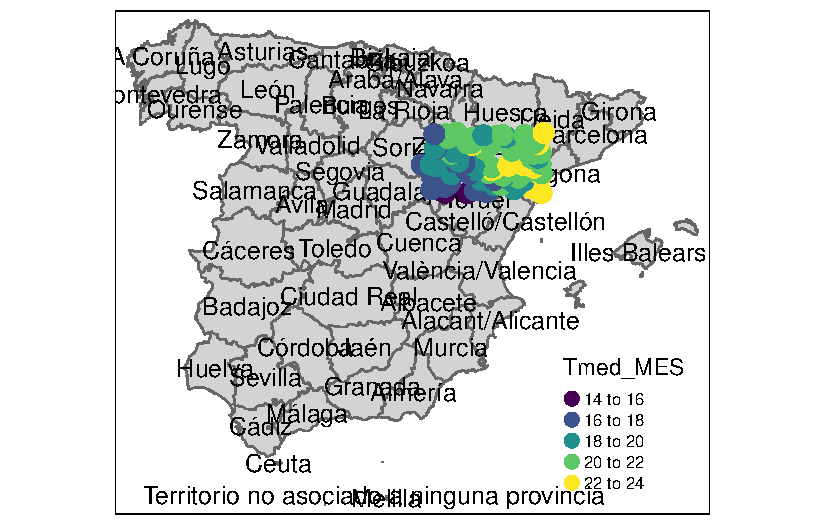
\includegraphics{01_RegresionLineal_files/figure-pdf/unnamed-chunk-15-1.pdf}

}

\end{figure}

\begin{verbatim}
integer(0)
\end{verbatim}

En contra de lo que cabría esperar, si ploteamos directamente el objeto
de la regresión no nos dará la gráfica de arriba, sino que nos da una
serie de gráficos sobre los residuos, que veremos más adelante.

\begin{Shaded}
\begin{Highlighting}[]
\FunctionTok{plot}\NormalTok{(mod\_lm)}
\end{Highlighting}
\end{Shaded}

\begin{figure}[H]

{\centering \includegraphics{01_RegresionLineal_files/figure-pdf/unnamed-chunk-16-1.pdf}

}

\end{figure}

\begin{figure}[H]

{\centering \includegraphics{01_RegresionLineal_files/figure-pdf/unnamed-chunk-16-2.pdf}

}

\end{figure}

\begin{figure}[H]

{\centering \includegraphics{01_RegresionLineal_files/figure-pdf/unnamed-chunk-16-3.pdf}

}

\end{figure}

\begin{figure}[H]

{\centering \includegraphics{01_RegresionLineal_files/figure-pdf/unnamed-chunk-16-4.pdf}

}

\end{figure}

\begin{quote}
\textbf{Sobre la visualización de los datos} Ya hemos comentado varias
veces la importancia de visualizar nuestros datos antes de extraer
ninguna conclusión de ellos. Hay una cierta tendencia a considerar que
una simple visualización no aporta demasiado, ya que sólo podemos llegar
a conclusiones cualitativas, mientras que un análisis de correlación o
regresión es \emph{estadística} y por tanto nos proporcionan información
numérica que podemos cuantificar (¿es la variable significativa?). Sin
embargo, no debemos NUNCA interpretar los resultados de un análisis sin
visualizar los datos. Un ejemplo de esto es el cuarteto de Anscombe,
creado en 1973 por el estadístico británico Francis Anscombe. Se trata
de cuatro datasets que contienen cada uno una variable \texttt{x} y una
\texttt{y}. Podemos acceder a ellos mediante el paquete
\texttt{datasets}, con la instrucción \texttt{library(datasets)} y
tecleando a continuación \texttt{anscombe} Para comprobar qué tiene de
particular este dataset, realizad lo siguiente: 1. Calculad la media y
desviación típica de todas las \texttt{x}, y de todas las \texttt{y} 2.
Calculad la correlación entre \texttt{x} e \texttt{y} para los cuatro
datasets 3. Ajustad un modelo lineal para cada par de \texttt{x} e
\texttt{y} 4. Representad visualmente cada pareja de \texttt{x} e
\texttt{y} ¿Qué observamos?
\end{quote}

\hypertarget{haciendo-predicciones-a-partir-de-nuestro-modelo}{%
\subsection{Haciendo predicciones a partir de nuestro
modelo}\label{haciendo-predicciones-a-partir-de-nuestro-modelo}}

Uno de los objetivos principales de la regresión es conocer la ecuación
que relaciona la variable dependiente con la independiente, de manera
que podamos predecir, para cualquier valor de \(x\), cual sería el valor
de \(y\) esperado.

Para hacer predicciones, podríamos simplemente construir una nueva
variable usando los coeficientes obtenidos de la regresión:

\begin{Shaded}
\begin{Highlighting}[]
\FunctionTok{coef}\NormalTok{(mod\_lm)}
\end{Highlighting}
\end{Shaded}

\begin{verbatim}
 (Intercept)    elevation 
21.923433399 -0.005710663 
\end{verbatim}

\begin{Shaded}
\begin{Highlighting}[]
\NormalTok{predicciones }\OtherTok{\textless{}{-}} \FloatTok{21.923433} \SpecialCharTok{{-}} \FloatTok{0.005711}\SpecialCharTok{*}\NormalTok{meteo}\SpecialCharTok{$}\NormalTok{elevation}
\NormalTok{predicciones}
\end{Highlighting}
\end{Shaded}

\begin{verbatim}
  [1] 13.79668 15.64133 14.90461 12.72872 13.91661 16.08679 16.88633 17.19472
  [9] 14.45344 15.15019 18.55965 18.94229 21.24382 21.79779 21.79779 21.46655
 [17] 21.80350 17.26326 21.78637 14.19645 15.37863 16.06395 16.25241 16.44658
 [25] 14.29925 14.53340 19.54195 20.82121 15.44716 20.51282 20.43286 21.91201
 [33] 21.72355 21.84919 21.02109 21.80921 21.42658 15.36149 21.28951 19.43344
 [41] 20.31293 18.97085 16.97771 17.33179 18.63961 19.58192 19.48484 20.30151
 [49] 14.99028 15.16732 16.52083 16.84635 16.82351 16.93202 17.31466 17.34321
 [57] 16.11535 16.27525 17.50312 17.92573 17.82294 19.15360 19.42773 17.78867
 [65] 19.02796 18.31979 19.31922 18.59392 16.05824 17.88004 18.26268 18.91374
 [73] 19.19357 19.47341 18.45115 18.95942 19.80465 20.25582 18.37690 18.37690
 [81] 18.77096 19.02224 18.78809 19.38775 18.61105 18.91945 18.94229 19.06793
 [89] 19.15360 16.85206 16.92060 20.05594 20.20442 20.33006 20.43286 20.31864
 [97] 20.43286 20.31864 17.86291 19.57050 19.94743 20.30722 19.30208 19.69043
[105] 19.69043 20.62704 17.38890 19.45628 20.35291 17.61734 19.48484 20.31864
[113] 19.44486 20.71841 17.67445 15.60136 17.75440 18.43972 16.13819 14.49913
[121] 15.13876 14.82466 17.60021 19.47912 16.99484 18.52539 19.73041 19.95314
[129] 18.51397 20.60419 18.39403 20.74126 20.73554 14.29925 15.90975 17.09193
[137] 16.99484 17.53167 16.82922 18.03424 18.99369 19.17073 18.78238 18.73669
[145] 19.73041 17.49741 19.75896 19.86747 19.71328 20.41573 20.53566 20.68415
[153] 19.75896 19.74183 21.05536 17.12619 17.02911 18.77667 16.50369 16.51512
[161] 18.62247 20.14731 20.33577 20.70699 18.47970 14.69331 15.68702 16.09250
[169] 14.95601 18.19415 19.31922 20.15873 21.16958 21.09534 20.39860 18.97656
[177] 19.98740 20.79265 20.86119 20.31864 15.74413 18.97656 18.89660 19.05651
[185] 18.69101 12.87150 19.12504 18.26839 18.50825 19.45628 20.05022 20.00454
[193] 20.07307 17.66874 20.51282 20.56993 19.26782 19.74754 18.83378 20.52995
[201] 20.52995 18.88518 16.08679 19.42773 19.86747 19.85034 20.18158 19.75896
[209] 19.81036 19.81036 20.09591 20.55850 20.15873 20.34720 21.15816 19.23355
[217] 17.84578 18.93087 20.23298 19.04509 20.87261 19.39346 21.75210 19.10220
[225] 21.73497 19.86176 20.64417 20.23298 21.60933 15.29296 16.12106 16.07537
[233] 16.19530 15.47571
\end{verbatim}

Sin embargo, \texttt{R} incluye la función \texttt{predict()} que hace
esto por nosotros automáticamente, lo cual es muy útil sobre todo en el
caso de regresiones múltiples. \texttt{predict()} necesita que le demos
dos inputs:

\begin{itemize}
\tightlist
\item
  un objeto de regresión (en este caso \texttt{mod\_lm})
\item
  una tabla o data frame que contenga todas y cada una de las variables
  explicativas usadas para ajustar el modelo
\end{itemize}

Lo que hace \texttt{predict()} es, para cada fila de la tabla que le
indiquemos, calcular el valor de \(y\) usando los valores de las
diferentes \(x\) para esa fila y los coeficientes estimados por el
modelo. En el caso de la regresión simple, \texttt{mod\_lm} calculará el
valor de temperatura media para cada valor de altitud que contenga la
tabla:

\begin{Shaded}
\begin{Highlighting}[]
\FunctionTok{predict}\NormalTok{(mod\_lm, meteo)}
\end{Highlighting}
\end{Shaded}

\begin{verbatim}
       1        2        3        4        5        6        7        8 
13.79716 15.64170 14.90503 12.72927 13.91708 16.08714 16.88663 17.19500 
       9       10       11       12       13       14       15       16 
14.45389 15.15059 18.55985 18.94247 21.24386 21.79780 21.79780 21.46658 
      17       18       19       20       21       22       23       24 
21.80351 17.26353 21.78638 14.19691 15.37901 16.06429 16.25275 16.44691 
      25       26       27       28       29       30       31       32 
14.29970 14.53384 19.54209 20.82128 15.44754 20.51290 20.43295 21.91201 
      33       34       35       36       37       38       39       40 
21.72356 21.84919 21.02115 21.80922 21.42661 15.36188 21.28955 19.43358 
      41       42       43       44       45       46       47       48 
20.31303 18.97102 16.97800 17.33206 18.63980 19.58206 19.48498 20.30161 
      49       50       51       52       53       54       55       56 
14.99069 15.16772 16.52115 16.84665 16.82381 16.93231 17.31493 17.34348 
      57       58       59       60       61       62       63       64 
16.11569 16.27559 17.50338 17.92597 17.82318 19.15376 19.42787 17.78891 
      65       66       67       68       69       70       71       72 
19.02813 18.32001 19.31937 18.59412 16.05858 17.88028 18.26290 18.91391 
      73       74       75       76       77       78       79       80 
19.19374 19.47356 18.45135 18.95960 19.80478 20.25592 18.37711 18.37711 
      81       82       83       84       85       86       87       88 
18.77115 19.02242 18.78828 19.38790 18.61125 18.91962 18.94247 19.06810 
      89       90       91       92       93       94       95       96 
19.15376 16.85236 16.92089 20.05605 20.20452 20.33016 20.43295 20.31874 
      97       98       99      100      101      102      103      104 
20.43295 20.31874 17.86315 19.57064 19.94754 20.30732 19.30224 19.69056 
     105      106      107      108      109      110      111      112 
19.69056 20.62711 17.38917 19.45643 20.35300 17.61759 19.48498 20.31874 
     113      114      115      116      117      118      119      120 
19.44501 20.71848 17.67470 15.60173 17.75465 18.43993 16.13853 14.49957 
     121      122      123      124      125      126      127      128 
15.13917 14.82508 17.60046 19.47927 16.99513 18.52559 19.73054 19.95325 
     129      130      131      132      133      134      135      136 
18.51417 20.60427 18.39424 20.74133 20.73562 14.29970 15.91011 17.09221 
     137      138      139      140      141      142      143      144 
16.99513 17.53193 16.82952 18.03447 18.99386 19.17089 18.78257 18.73688 
     145      146      147      148      149      150      151      152 
19.73054 17.49767 19.75909 19.86759 19.71341 20.41582 20.53574 20.68422 
     153      154      155      156      157      158      159      160 
19.75909 19.74196 21.05541 17.12648 17.02940 18.77686 16.50401 16.51544 
     161      162      163      164      165      166      167      168 
18.62267 20.14742 20.33587 20.70706 18.47990 14.69373 15.68739 16.09285 
     169      170      171      172      173      174      175      176 
14.95642 18.19437 19.31937 20.15884 21.16963 21.09539 20.39869 18.97673 
     177      178      179      180      181      182      183      184 
19.98752 20.79272 20.86125 20.31874 15.74450 18.97673 18.89678 19.05668 
     185      186      187      188      189      190      191      192 
18.69120 12.87203 19.12521 18.26861 18.50846 19.45643 20.05034 20.00465 
     193      194      195      196      197      198      199      200 
20.07318 17.66899 20.51290 20.57001 19.26798 19.74767 18.83396 20.53003 
     201      202      203      204      205      206      207      208 
20.53003 18.88536 16.08714 19.42787 19.86759 19.85046 20.18168 19.75909 
     209      210      211      212      213      214      215      216 
19.81049 19.81049 20.09602 20.55858 20.15884 20.34729 21.15820 19.23371 
     217      218      219      220      221      222      223      224 
17.84602 18.93105 20.23308 19.04526 20.87267 19.39361 21.75211 19.10237 
     225      226      227      228      229      230      231      232 
21.73498 19.86188 20.64424 20.23308 21.60935 15.29335 16.12140 16.07571 
     233      234 
16.19564 15.47609 
\end{verbatim}

Incluso podemos guardar estas predicciones como una columna más de
\texttt{meteo}:

\begin{Shaded}
\begin{Highlighting}[]
\NormalTok{meteo}\SpecialCharTok{$}\NormalTok{pred }\OtherTok{\textless{}{-}}  \FunctionTok{predict}\NormalTok{(mod\_lm, meteo)}

\FunctionTok{head}\NormalTok{(meteo)}
\end{Highlighting}
\end{Shaded}

\begin{verbatim}
# A tibble: 6 x 8
  TavgMAX  Tavg   long  d_atl d_medit     lat elevation  pred
    <dbl> <dbl>  <dbl>  <dbl>   <dbl>   <dbl>     <dbl> <dbl>
1    20.3  14.6 614350 305753  152147 4489750      1423  13.8
2    23.8  16.1 593950 271251  183121 4522150      1100  15.6
3    24.4  18.2 567250 279823  204123 4512650      1229  14.9
4    20.1  14.0 609150 319257  150357 4475450      1610  12.7
5    20.3  13.8 629450 306673  138390 4491350      1402  13.9
6    21.9  16.2 666750 317312  103530 4489850      1022  16.1
\end{verbatim}

Ahora podríamos hacer un gráfico que compare los valores predichos y los
observados:

\begin{Shaded}
\begin{Highlighting}[]
\FunctionTok{plot}\NormalTok{(meteo}\SpecialCharTok{$}\NormalTok{Tavg, meteo}\SpecialCharTok{$}\NormalTok{pred)}
\end{Highlighting}
\end{Shaded}

\begin{figure}[H]

{\centering \includegraphics{01_RegresionLineal_files/figure-pdf/unnamed-chunk-20-1.pdf}

}

\end{figure}

Lo interesante de la función \texttt{predict()} es que no hace falta
aplicarla a la misma tabla de datos que hemos usado para ajustar el
modelo, sino que si tenemos una serie de datos nueva (de otras
estaciones, u otras fechas) también podemos calcular el valor predicho
por el modelo. En este caso, para cualquier punto del que tengamos la
altitud, podemos determinar la temperatura media. Abramos el otro
fichero que teníamos disponible en el campus virtual, llamado
\texttt{meteo\_nuevo.txt}:

\begin{Shaded}
\begin{Highlighting}[]
\NormalTok{meteo2 }\OtherTok{\textless{}{-}} \FunctionTok{read\_delim}\NormalTok{(}\StringTok{"./data/meteo/meteo\_nuevo.txt"}\NormalTok{, }\StringTok{"}\SpecialCharTok{\textbackslash{}t}\StringTok{"}\NormalTok{)}
\end{Highlighting}
\end{Shaded}

\begin{verbatim}
Rows: 100 Columns: 2
-- Column specification --------------------------------------------------------
Delimiter: "\t"
dbl (2): elevation, d_medit

i Use `spec()` to retrieve the full column specification for this data.
i Specify the column types or set `show_col_types = FALSE` to quiet this message.
\end{verbatim}

\begin{Shaded}
\begin{Highlighting}[]
\NormalTok{meteo2}
\end{Highlighting}
\end{Shaded}

\begin{verbatim}
# A tibble: 100 x 2
   elevation d_medit
       <dbl>   <dbl>
 1      793.  204153
 2      864.  193620
 3      939.  209678
 4      706.  221949
 5      787.  210552
 6      934.  188943
 7      802.  222480
 8     1061.  203576
 9      836.  219916
10      735.  202829
# i 90 more rows
\end{verbatim}

Vemos que es una tabla que contiene valores de altitud y distancia al
mediterráneo, pero no contiene de hecho valores de temperatura. En base
al modelo que ajustamos antes, podemos generarlos con
\texttt{predict()}:

\begin{Shaded}
\begin{Highlighting}[]
\NormalTok{meteo2}\SpecialCharTok{$}\NormalTok{temp }\OtherTok{\textless{}{-}} \FunctionTok{predict}\NormalTok{(mod\_lm, meteo2)}
\NormalTok{meteo2}
\end{Highlighting}
\end{Shaded}

\begin{verbatim}
# A tibble: 100 x 3
   elevation d_medit  temp
       <dbl>   <dbl> <dbl>
 1      793.  204153  17.4
 2      864.  193620  17.0
 3      939.  209678  16.6
 4      706.  221949  17.9
 5      787.  210552  17.4
 6      934.  188943  16.6
 7      802.  222480  17.3
 8     1061.  203576  15.9
 9      836.  219916  17.1
10      735.  202829  17.7
# i 90 more rows
\end{verbatim}

Esta opción es muy interesante, ya que cuando generamos una ecuación de
regresión, raramente queremos aplicarla sobre los datos ya observados,
sino que querremos usarla para predecir valores en aquellos lugares
donde no tengamos medidas.

\begin{quote}
\textbf{Consejo:}Debemos ser responsables, sin embargo, de no extrapolar
más allá de lo lógico: si el modelo de regresión se ha ajustado con
datos del valle del Ebro, ¿tiene sentido aplicarlos en Galicia?
\end{quote}

\hypertarget{regresiuxf3n-lineal-muxfaltiple}{%
\section{Regresión lineal
múltiple}\label{regresiuxf3n-lineal-muxfaltiple}}

De la misma manera que ajustamos una regresión lineal simple, podemos
ajustar una múltiple, simplemente añadiendo más variables independientes
a la derecha de la fórmula, después del \texttt{\textasciitilde{}}:

\begin{Shaded}
\begin{Highlighting}[]
\NormalTok{mod\_mult }\OtherTok{\textless{}{-}} \FunctionTok{lm}\NormalTok{(Tavg }\SpecialCharTok{\textasciitilde{}}\NormalTok{ d\_atl }\SpecialCharTok{+}\NormalTok{ d\_medit }\SpecialCharTok{+}\NormalTok{ elevation, }\AttributeTok{data =}\NormalTok{ meteo)}
\NormalTok{mod\_mult}
\end{Highlighting}
\end{Shaded}

\begin{verbatim}

Call:
lm(formula = Tavg ~ d_atl + d_medit + elevation, data = meteo)

Coefficients:
(Intercept)        d_atl      d_medit    elevation  
  2.156e+01    3.749e-06   -3.393e-06   -5.545e-03  
\end{verbatim}

A efectos prácticos, el modelo múltiple y el simple son prácticamente
iguales, aunque en este caso la función \texttt{summary} nos da la
significación de cada una de las variables:

\begin{Shaded}
\begin{Highlighting}[]
\FunctionTok{summary}\NormalTok{(mod\_mult)}
\end{Highlighting}
\end{Shaded}

\begin{verbatim}

Call:
lm(formula = Tavg ~ d_atl + d_medit + elevation, data = meteo)

Residuals:
    Min      1Q  Median      3Q     Max 
-4.8514 -0.5623  0.0526  0.6173  3.1647 

Coefficients:
              Estimate Std. Error t value Pr(>|t|)    
(Intercept)  2.156e+01  9.105e-01  23.676   <2e-16 ***
d_atl        3.749e-06  2.404e-06   1.560    0.120    
d_medit     -3.393e-06  2.846e-06  -1.192    0.235    
elevation   -5.545e-03  2.136e-04 -25.959   <2e-16 ***
---
Signif. codes:  0 '***' 0.001 '**' 0.01 '*' 0.05 '.' 0.1 ' ' 1

Residual standard error: 0.982 on 230 degrees of freedom
Multiple R-squared:  0.8257,    Adjusted R-squared:  0.8235 
F-statistic: 363.3 on 3 and 230 DF,  p-value: < 2.2e-16
\end{verbatim}

Vemos que la R2 del modelo ha mejorado de forma sustancial. Pero
recordemos que se considera el efecto de una variable como no
significativo si el p-valor asociado a ella es mayor de 0.05. Eso quiere
decir que el riesgo de rechazar la hipótesis nula (el riesgo de asumir
una relación cuando no la hay) es demasiado alto, y por tanto no la
rechazamos. En este caso, vemos que ni la distancia al Mediterráneo ni
la distancia al Atlántico resultan significativas. Según lo visto en
clase, sería mejor eliminarlas, pero por otro lado nos hacen subir el R2
de manera muy clara. Probemos a quitar sólo una de ellas:

\begin{Shaded}
\begin{Highlighting}[]
\NormalTok{mod\_mult2 }\OtherTok{\textless{}{-}} \FunctionTok{lm}\NormalTok{(Tavg }\SpecialCharTok{\textasciitilde{}}\NormalTok{ d\_medit }\SpecialCharTok{+}\NormalTok{ elevation, }\AttributeTok{data =}\NormalTok{ meteo)}
\FunctionTok{summary}\NormalTok{(mod\_mult2)}
\end{Highlighting}
\end{Shaded}

\begin{verbatim}

Call:
lm(formula = Tavg ~ d_medit + elevation, data = meteo)

Residuals:
    Min      1Q  Median      3Q     Max 
-4.7490 -0.5785  0.0227  0.5727  3.3712 

Coefficients:
              Estimate Std. Error t value Pr(>|t|)    
(Intercept)  2.296e+01  1.595e-01  143.88   <2e-16 ***
d_medit     -7.675e-06  7.528e-07  -10.20   <2e-16 ***
elevation   -5.378e-03  1.856e-04  -28.98   <2e-16 ***
---
Signif. codes:  0 '***' 0.001 '**' 0.01 '*' 0.05 '.' 0.1 ' ' 1

Residual standard error: 0.985 on 231 degrees of freedom
Multiple R-squared:  0.8239,    Adjusted R-squared:  0.8224 
F-statistic: 540.3 on 2 and 231 DF,  p-value: < 2.2e-16
\end{verbatim}

¡Ahora sí que la distancia al Mediterráneo resulta significativa, y la
R2 del modelo (0.82) sigue siendo muy superior a la del modelo simple
(0.74). Lo curioso es que si hubiéramos eliminado \texttt{d\_medit},
también sería significativa \texttt{d\_atl} (podéis hacer la prueba)
¿Qué puede estar pasando?

Lo que estamos viendo es un ejemplo de multicolinealidad. Como la
distancia al Mediterráneo y al Atlántico están muy relacionadas (si
aumenta una, disminuye la otra), si introducimos las dos en el modelo
este no es capaz de distinguir el efecto de cada una de ellas, y
concluye que no tienen efecto. De hecho, veamos como de correlacionadas
están estas dos variables:

\begin{Shaded}
\begin{Highlighting}[]
\FunctionTok{cor}\NormalTok{(meteo}\SpecialCharTok{$}\NormalTok{d\_atl, meteo}\SpecialCharTok{$}\NormalTok{d\_medit)}
\end{Highlighting}
\end{Shaded}

\begin{verbatim}
[1] -0.9525821
\end{verbatim}

Por tanto, dejaremos sólo una de ellas en el modelo, en este caso la
distancia al Mediterráneo. Lo interesante es que podemos predecir
temperaturas en nuestra tabla de nuevos valores, usando el modelo de
regresión múltiple:

\begin{Shaded}
\begin{Highlighting}[]
\FunctionTok{predict}\NormalTok{(mod\_mult2, meteo2)}
\end{Highlighting}
\end{Shaded}

\begin{verbatim}
       1        2        3        4        5        6        7        8 
17.12514 16.82208 16.29817 17.45700 17.10434 16.48407 16.93618 15.68594 
       9       10       11       12       13       14       15       16 
16.76974 17.44436 18.06764 16.64387 17.27120 16.09408 16.66035 17.05316 
      17       18       19       20       21       22       23       24 
16.14305 14.78709 15.94748 15.39889 20.87385 16.08418 16.61257 17.58826 
      25       26       27       28       29       30       31       32 
16.22689 16.74222 17.28661 14.11201 17.53732 19.11453 14.50081 14.66675 
      33       34       35       36       37       38       39       40 
18.31549 18.71684 13.93286 18.06864 17.19598 19.16897 15.03308 16.40134 
      41       42       43       44       45       46       47       48 
16.58971 16.81448 17.25677 16.16466 16.32135 16.86009 15.64677 17.75046 
      49       50       51       52       53       54       55       56 
14.12446 17.88584 14.74712 16.78598 17.13428 16.43328 18.71701 16.22936 
      57       58       59       60       61       62       63       64 
16.38941 18.04153 17.36000 18.77970 15.24015 17.34046 17.37639 13.99712 
      65       66       67       68       69       70       71       72 
14.95117 18.21192 18.30910 18.33676 16.91608 18.87682 17.01177 15.09166 
      73       74       75       76       77       78       79       80 
18.54233 19.18103 13.98042 17.05097 15.85675 18.48408 17.58232 16.75660 
      81       82       83       84       85       86       87       88 
16.20362 12.84291 16.13229 19.39104 18.98500 17.45716 15.43576 18.05760 
      89       90       91       92       93       94       95       96 
15.81553 17.08892 17.60376 18.81896 15.97251 16.41554 16.04488 17.89542 
      97       98       99      100 
15.21175 17.32653 18.20423 16.26098 
\end{verbatim}

Esto funcionará siempre que la tabla que proporcionemos contenga todas y
cada una de las variables explicativas del modelo. Si intentamos
predecir con el modelo que contiene \texttt{d\_atl}, recibiremos este
mensaje de error:

\begin{Shaded}
\begin{Highlighting}[]
\FunctionTok{predict}\NormalTok{(mod\_mult, meteo2)}
\end{Highlighting}
\end{Shaded}

\begin{verbatim}
Error in eval(predvars, data, env): objeto 'd_atl' no encontrado
\end{verbatim}

\hypertarget{testando-las-asunciones-del-modelo}{%
\section{Testando las asunciones del
modelo}\label{testando-las-asunciones-del-modelo}}

Hemos visto que los modelos lineales deben cumplir básicamente cuatro
criterios:

\hypertarget{linealidad}{%
\subsection{Linealidad}\label{linealidad}}

la linealidad entre predictores y variable dependiente se puede evaluar
gráficamente. En este caso, la relación entre la cota y la temperatura
parece claramente lineal, como ya habíamos visto antes:

\begin{Shaded}
\begin{Highlighting}[]
\FunctionTok{plot}\NormalTok{(meteo}\SpecialCharTok{$}\NormalTok{elevation, meteo}\SpecialCharTok{$}\NormalTok{Tavg)}
\end{Highlighting}
\end{Shaded}

\begin{figure}[H]

{\centering \includegraphics{01_RegresionLineal_files/figure-pdf/unnamed-chunk-29-1.pdf}

}

\end{figure}

\hypertarget{independencia}{%
\subsection{Independencia}\label{independencia}}

Las observaciones deben ser independientes unas de otras (por eso se
llaman variables independientes). Aunque una parte importante de la
evaluación de la independencia la podemos inferir si conocemos bien la
muestra, la gráfica de predichos y residuos nos puede dar también
información importante. Ambos los podemos extraer del objeto \texttt{lm}
que hayamos guardado, usando las funciones \texttt{fitted()} y
\texttt{residuals()}, respectivamente:

\begin{Shaded}
\begin{Highlighting}[]
\NormalTok{predichos }\OtherTok{\textless{}{-}} \FunctionTok{fitted}\NormalTok{(mod\_lm)}
\NormalTok{residuos }\OtherTok{\textless{}{-}} \FunctionTok{residuals}\NormalTok{(mod\_lm)}

\FunctionTok{plot}\NormalTok{(predichos, residuos)}
\end{Highlighting}
\end{Shaded}

\begin{figure}[H]

{\centering \includegraphics{01_RegresionLineal_files/figure-pdf/unnamed-chunk-30-1.pdf}

}

\end{figure}

No parece presentar mayores problemas.

\hypertarget{homocedasticidad}{%
\subsection{Homocedasticidad}\label{homocedasticidad}}

Otro importante criterio que debe seguir un modelo lineal es el de ser
homocedástico. Esto quiere decir que los residuos son independientes a
los valores de la variable explicativa. O dicho de otra manera, que la
varianza del error es constante a lo largo de las observaciones. Lo
podemos ver con la misma gráfica de antes:

\begin{Shaded}
\begin{Highlighting}[]
\FunctionTok{plot}\NormalTok{(predichos, residuos)}
\end{Highlighting}
\end{Shaded}

\begin{figure}[H]

{\centering \includegraphics{01_RegresionLineal_files/figure-pdf/unnamed-chunk-31-1.pdf}

}

\end{figure}

\hypertarget{normalidad}{%
\subsection{Normalidad}\label{normalidad}}

Para evaluar la normalidad de los residuos podemos usar varias gráficas:

\begin{itemize}
\tightlist
\item
  Histogramas
\end{itemize}

Usaremos la función \texttt{hist()}, sobre los residuos del modelo (que
se obtienen con la función \texttt{residuals()}):

\begin{Shaded}
\begin{Highlighting}[]
\FunctionTok{hist}\NormalTok{(}\FunctionTok{residuals}\NormalTok{(mod\_lm))}
\end{Highlighting}
\end{Shaded}

\begin{figure}[H]

{\centering \includegraphics{01_RegresionLineal_files/figure-pdf/unnamed-chunk-32-1.pdf}

}

\end{figure}

\begin{itemize}
\tightlist
\item
  Boxplot
\end{itemize}

Mediante la función \texttt{boxplot()} podemos construir un diagrama de
cajas con cualquier variable (en este caso, recordad que se debe hacer
sobre los residuos):

\begin{Shaded}
\begin{Highlighting}[]
\FunctionTok{boxplot}\NormalTok{(}\FunctionTok{residuals}\NormalTok{(mod\_lm), }\AttributeTok{col =} \StringTok{"steelblue"}\NormalTok{)}
\end{Highlighting}
\end{Shaded}

\begin{figure}[H]

{\centering \includegraphics{01_RegresionLineal_files/figure-pdf/unnamed-chunk-33-1.pdf}

}

\end{figure}

\begin{itemize}
\tightlist
\item
  QQplot
\end{itemize}

\begin{Shaded}
\begin{Highlighting}[]
\FunctionTok{qqnorm}\NormalTok{(}\FunctionTok{residuals}\NormalTok{(mod\_lm), }\AttributeTok{pch =} \DecValTok{1}\NormalTok{, }\AttributeTok{frame =} \ConstantTok{FALSE}\NormalTok{)}
\FunctionTok{qqline}\NormalTok{(}\FunctionTok{residuals}\NormalTok{(mod\_lm), }\AttributeTok{col =} \StringTok{"steelblue"}\NormalTok{, }\AttributeTok{lwd =} \DecValTok{2}\NormalTok{)}
\end{Highlighting}
\end{Shaded}

\begin{figure}[H]

{\centering \includegraphics{01_RegresionLineal_files/figure-pdf/unnamed-chunk-34-1.pdf}

}

\end{figure}

Todas estas gráficas parecen estar razonablemente bien. Si queremos una
evaluación más cuantitativa, también podemos usar tests para saber si
los residuos están normalmente distribuidos o no. Un ejemplo es el test
de Shapiro-Wilk:

\begin{Shaded}
\begin{Highlighting}[]
\FunctionTok{shapiro.test}\NormalTok{(}\FunctionTok{residuals}\NormalTok{(mod\_lm))}
\end{Highlighting}
\end{Shaded}

\begin{verbatim}

    Shapiro-Wilk normality test

data:  residuals(mod_lm)
W = 0.99415, p-value = 0.4982
\end{verbatim}

En este caso, la hipótesis nula del test de Shapiro-Wilk es que la
distribución de la variable testada es normal. Por lo tanto, si el
resultado del test es no significativo quiere decir que no podemos
rechazar la hipótesis nula, es decir, que no podemos rechazar que la
distribución sea normal (en definitiva, que sí que es normal).

Por supuesto, esta lógica funciona al contrario: si el resultado del
test de Shapiro-Wilk es significativo, quiere decir que la variable que
estamos testando (en este caso los residuos), no siguen una distribución
normal.

\begin{quote}
\textbf{Sobre los tests de normalidad} Además del test de Shapiro-Wilk
existen otros tests para evaluar de manera estadística si una variable
sigue una distribución normal. Aunque se pueden usar para tomar
decisiones respecto a un modelo, hay que hacerlo sabiendo que la mayoría
de estos tests son muy estrictos. Es decir, que incluso una ligera
desviación respecto de la normalidad resultará en significación del
test. Debemos tener sentido común para decidir si esto invalida nuestro
modelo o no, como hemos visto durante las clases teóricas:
\end{quote}

Por otro lado, como hemos indicado antes, algunas de las gráficas de
evaluación de los supuestos del modelo nos los da directamente R
mediante el ploteo del objeto \texttt{lm}:

\begin{Shaded}
\begin{Highlighting}[]
\FunctionTok{plot}\NormalTok{(mod\_lm)}
\end{Highlighting}
\end{Shaded}

\begin{figure}[H]

{\centering \includegraphics{01_RegresionLineal_files/figure-pdf/unnamed-chunk-36-1.pdf}

}

\end{figure}

\begin{figure}[H]

{\centering \includegraphics{01_RegresionLineal_files/figure-pdf/unnamed-chunk-36-2.pdf}

}

\end{figure}

\begin{figure}[H]

{\centering \includegraphics{01_RegresionLineal_files/figure-pdf/unnamed-chunk-36-3.pdf}

}

\end{figure}

\begin{figure}[H]

{\centering \includegraphics{01_RegresionLineal_files/figure-pdf/unnamed-chunk-36-4.pdf}

}

\end{figure}

En concreto nos interesan los dos primeros: un scatterplot de residuos
vs.~predichos, y un qqplot con los residuos. Con ellos podemos testar al
menos 3 de las 4 asunciones.

\hypertarget{regresiuxf3n-usando-variables-espacialmente-continuas}{%
\section{Regresión usando variables espacialmente
continuas}\label{regresiuxf3n-usando-variables-espacialmente-continuas}}

Hemos visto que la función \texttt{predict()} permite calcular la
variable dependiente en función de las variables explicativas. Pero aún
más, si tenemos un mapa continuo con los valores de las variables
explicativas, \texttt{predict()} nos permitirá generar un raster
continuo de predicciones espacializadas. Veamos un ejemplo.

En este caso, tenemos una serie de rasters de una zona de estudio, y que
corresponden con las variables que hemos usado antes para ajustar el
modelo: altitud, distancia al Atlántico y distancia al Mediterráneo. Lo
primero es cargar los tres rasters, para lo que necesitaremos la
librería \texttt{terra} y su función \texttt{rast()}:

\begin{Shaded}
\begin{Highlighting}[]
\FunctionTok{library}\NormalTok{(terra)}
\end{Highlighting}
\end{Shaded}

\begin{verbatim}
Warning: package 'terra' was built under R version 4.2.3
\end{verbatim}

\begin{verbatim}
terra 1.7.71
\end{verbatim}

\begin{verbatim}

Attaching package: 'terra'
\end{verbatim}

\begin{verbatim}
The following object is masked from 'package:tidyr':

    extract
\end{verbatim}

\begin{Shaded}
\begin{Highlighting}[]
\NormalTok{elevation }\OtherTok{\textless{}{-}} \FunctionTok{rast}\NormalTok{(}\StringTok{"./data/meteo/meteo\_espacial/rasters\_meteo/elevation.txt"}\NormalTok{)}
\NormalTok{d\_atl }\OtherTok{\textless{}{-}} \FunctionTok{rast}\NormalTok{(}\StringTok{"./data/meteo/meteo\_espacial/rasters\_meteo/d\_atl.txt"}\NormalTok{)}
\NormalTok{d\_medit }\OtherTok{\textless{}{-}} \FunctionTok{rast}\NormalTok{(}\StringTok{"./data/meteo/meteo\_espacial/rasters\_meteo/d\_medit.txt"}\NormalTok{)}
\end{Highlighting}
\end{Shaded}

Podemos visualizarlos de manera sencilla con \texttt{plot()}:

\begin{Shaded}
\begin{Highlighting}[]
\FunctionTok{plot}\NormalTok{(elevation)}
\end{Highlighting}
\end{Shaded}

\begin{figure}[H]

{\centering \includegraphics{01_RegresionLineal_files/figure-pdf/unnamed-chunk-38-1.pdf}

}

\end{figure}

\begin{Shaded}
\begin{Highlighting}[]
\FunctionTok{plot}\NormalTok{(d\_atl)}
\end{Highlighting}
\end{Shaded}

\begin{figure}[H]

{\centering \includegraphics{01_RegresionLineal_files/figure-pdf/unnamed-chunk-38-2.pdf}

}

\end{figure}

\begin{Shaded}
\begin{Highlighting}[]
\FunctionTok{plot}\NormalTok{(d\_medit)}
\end{Highlighting}
\end{Shaded}

\begin{figure}[H]

{\centering \includegraphics{01_RegresionLineal_files/figure-pdf/unnamed-chunk-38-3.pdf}

}

\end{figure}

Ahora vamos a guardar esos 3 rasters en un único objeto, como si fuera
un raster multibanda. Este objeto se conoce como \texttt{stack}. Para
crearlo usaremos la función \texttt{c()}:

\begin{Shaded}
\begin{Highlighting}[]
\NormalTok{rasters }\OtherTok{\textless{}{-}} \FunctionTok{c}\NormalTok{(elevation, d\_atl, d\_medit)}
\end{Highlighting}
\end{Shaded}

Como los componentes del \texttt{stack} tienen los mismos nombres que
usamos para ajustar el modelo, podemos realizar predicciones usando los
valores continuos de los rasters. Cuando tecleemos \texttt{predict()} R
reconocerá que el input son rasters, y usará la función
\texttt{predict()} del paquete \texttt{terra}. La función
\texttt{predict()}del paquete \texttt{terra}se diferencia en el número y
orden de los argumentos. Primero hay que proporcionarle el
\texttt{SpatRaster} que contiene las variables, y después el modelo
ajustado - al revés de lo que hacíamos antes.

\begin{Shaded}
\begin{Highlighting}[]
\NormalTok{pred\_continua }\OtherTok{\textless{}{-}} \FunctionTok{predict}\NormalTok{(rasters, mod\_lm)}
\end{Highlighting}
\end{Shaded}

Ahora ya podemos representar las predicciones, que en este caso, como el
input era un raster, será también un raster:

\begin{Shaded}
\begin{Highlighting}[]
\FunctionTok{plot}\NormalTok{(pred\_continua)}
\end{Highlighting}
\end{Shaded}

\begin{figure}[H]

{\centering \includegraphics{01_RegresionLineal_files/figure-pdf/unnamed-chunk-41-1.pdf}

}

\end{figure}

Por supuesto, el procedimiento funcionaría exactamente igual con un
modelo de regresión múltiple:

\begin{Shaded}
\begin{Highlighting}[]
\NormalTok{pred\_cont\_multiple }\OtherTok{\textless{}{-}} \FunctionTok{predict}\NormalTok{(rasters, mod\_mult2)}
\FunctionTok{plot}\NormalTok{(pred\_cont\_multiple)}
\end{Highlighting}
\end{Shaded}

\begin{figure}[H]

{\centering \includegraphics{01_RegresionLineal_files/figure-pdf/unnamed-chunk-42-1.pdf}

}

\end{figure}

\hypertarget{sec-GLM}{%
\chapter{Regresión lineal generalizada (GLM) en R}\label{sec-GLM}}

\hypertarget{introducciuxf3n-los-modelos-lineales-generalizados-glms}{%
\section{Introducción: los modelos lineales generalizados
(GLMs)}\label{introducciuxf3n-los-modelos-lineales-generalizados-glms}}

Ya hemos visto en las clases teóricas que la regresión lineal
generalizada (o modelos lineales generalizados, GLM) son una alternativa
sólida a los casos en los que nuestra variable dependiente no sigue una
distribución normal, y por tanto, los residuos de la regresión lineal no
cumplirán los supuestos de la misma. Los GLM abordan estos problemas
flexibilizando la distribución de la variable respuesta, y conectándola
con un predictor lineal a través de una función de enlace (\emph{link
function}). Vamos a ver ahora ejemplos con algunas de las distribuciones
más habituales - más allá de la normal:

\hypertarget{regresiuxf3n-de-conteos-la-distribuciuxf3n-de-poisson}{%
\section{Regresión de conteos: la distribución de
Poisson}\label{regresiuxf3n-de-conteos-la-distribuciuxf3n-de-poisson}}

Uno de los casos más habituales en los que debemos usar los GLM es
cuando nuestra variable dependiente son conteos. En este caso seguirán
una distribución de Poisson, que se caracteriza como el número de veces
que un determinado evento ocurrirá en un intervalo de tiempo. Si es un
conteo de abundancia, por ejemplo, la variable dependiente será el
número de plantas (eventos) en un muestreo. La distribución de Poisson
tiene un sólo parámetro \(\lambda\), que es la media de eventos
esperada. Así, si generamos una serie de 100 observacions con
\(\lambda\) = 5:

\begin{Shaded}
\begin{Highlighting}[]
\NormalTok{poisson }\OtherTok{\textless{}{-}} \FunctionTok{rpois}\NormalTok{(}\DecValTok{500}\NormalTok{,}\DecValTok{5}\NormalTok{)}
\FunctionTok{hist}\NormalTok{(poisson, }\AttributeTok{breaks =} \DecValTok{20}\NormalTok{, }\AttributeTok{main =} \StringTok{"Histograma de dist. Poisson de media 5"}\NormalTok{, }\AttributeTok{xlab =} \StringTok{"Número de eventos"}\NormalTok{)}
\end{Highlighting}
\end{Shaded}

\begin{figure}[H]

{\centering \includegraphics{02_GLM_files/figure-pdf/unnamed-chunk-1-1.pdf}

}

\end{figure}

vemos que todos los valores son números enteros, ya que no puede haber,
lógicamente, valores como \emph{3,56 plantas}.

Para ajustar cualquier GLM usaremos la función \texttt{glm}, que viene
cargada por defecto en R y que tiene tres argumentos principales:

\begin{itemize}
\tightlist
\item
  \textbf{Formula}: la ecuación que define la variable dependiente y las
  independientes. Es igual que en la regresión lineal.
\item
  \textbf{data}: el data frame que contiene las variables
\item
  \textbf{family}: una descripción de la distribución que sigue el error
  y la función de enlace a usar. En el caso de conteos debe tomar el
  valor \texttt{"poisson"}
\end{itemize}

Vamos a ajustar una sencilla regresión Poisson usando datos de:

https://stats.idre.ucla.edu/stat/data/poisson\_sim.csv

En este ejemplo, \texttt{num\_awards} es el número de premios ganados
por los alumnos de un instituto en un año, \texttt{math} es una variable
continua que representa la nota obtenida por los estudiantes en el
examen final de matemáticas, y \texttt{prog} es una variable categórica
con tres niveles que indica el tipo de programa en el que están
matriculados: 1 = ``General'', 2 = ``Academic'' y 3 = ``Vocational''.

Como siempre, carguemos los datos y echémosles un vistazo:

\begin{Shaded}
\begin{Highlighting}[]
\NormalTok{premios }\OtherTok{\textless{}{-}} \FunctionTok{read.csv}\NormalTok{(}\StringTok{\textquotesingle{}https://stats.idre.ucla.edu/stat/data/poisson\_sim.csv\textquotesingle{}}\NormalTok{)}
\FunctionTok{str}\NormalTok{(premios)}
\end{Highlighting}
\end{Shaded}

\begin{verbatim}
'data.frame':   200 obs. of  4 variables:
 $ id        : int  45 108 15 67 153 51 164 133 2 53 ...
 $ num_awards: int  0 0 0 0 0 0 0 0 0 0 ...
 $ prog      : int  3 1 3 3 3 1 3 3 3 3 ...
 $ math      : int  41 41 44 42 40 42 46 40 33 46 ...
\end{verbatim}

\begin{Shaded}
\begin{Highlighting}[]
\FunctionTok{head}\NormalTok{(premios)}
\end{Highlighting}
\end{Shaded}

\begin{verbatim}
   id num_awards prog math
1  45          0    3   41
2 108          0    1   41
3  15          0    3   44
4  67          0    3   42
5 153          0    3   40
6  51          0    1   42
\end{verbatim}

Ahora podemos ajustar un modelo de Poisson. Para ello:

\begin{Shaded}
\begin{Highlighting}[]
\NormalTok{mod.poisson }\OtherTok{\textless{}{-}} \FunctionTok{glm}\NormalTok{(num\_awards }\SpecialCharTok{\textasciitilde{}}\NormalTok{ math }\SpecialCharTok{+}\NormalTok{ prog,  }\AttributeTok{data =}\NormalTok{ premios, }\AttributeTok{family =} \StringTok{"poisson"}\NormalTok{)}
\FunctionTok{summary}\NormalTok{(mod.poisson)}
\end{Highlighting}
\end{Shaded}

\begin{verbatim}

Call:
glm(formula = num_awards ~ math + prog, family = "poisson", data = premios)

Deviance Residuals: 
    Min       1Q   Median       3Q      Max  
-2.1840  -0.9003  -0.5891   0.3948   2.9539  

Coefficients:
             Estimate Std. Error z value Pr(>|z|)    
(Intercept) -5.578057   0.676823  -8.242   <2e-16 ***
math         0.086121   0.009586   8.984   <2e-16 ***
prog         0.123273   0.163261   0.755     0.45    
---
Signif. codes:  0 '***' 0.001 '**' 0.01 '*' 0.05 '.' 0.1 ' ' 1

(Dispersion parameter for poisson family taken to be 1)

    Null deviance: 287.67  on 199  degrees of freedom
Residual deviance: 203.45  on 197  degrees of freedom
AIC: 385.51

Number of Fisher Scoring iterations: 6
\end{verbatim}

\hypertarget{interpretando-los-resultados-de-un-glm-de-poisson}{%
\subsection{Interpretando los resultados de un GLM de
Poisson}\label{interpretando-los-resultados-de-un-glm-de-poisson}}

La salida de resultados cuando ejecutamos la orden \texttt{summary()} en
un GLM es muy parecida al de los modelos de regresión lineal, aunque con
algunos matices. Por ejemplo, ahora no nos proporciona el R2 del modelo,
ya que su cálculo no es posible. Además, si bien la significación de los
coeficientes estimados tiene la misma interpretación que en modelos
lineales (si p\textless{} 0.05 podemos rechazar que esa variable no
tenga un efecto), los valores de los coeficientes no pueden
interpretarse de manera directa.

Por ejemplo, en el modelo ajustado más arriba vemos que, cuanto mayor es
la nota en matemáticas, más premios han recibido, ya que el coeficiente
de \texttt{math} es positivo y altamente significativo. Pero no podemos
concluir que por cada punto que suba la nota de mates, se aumente en
0.086 el número de premios.

La manera de intepretar la salida es la siguiente: cuando \(x=0\),
entonces el valor esperado es la media de \(y\) y toma una valor de
\(e^\alpha\), donde \(\alpha\) es el intercepto. Con cada unidad de
incremento en \(x\), el valor predicho tiene un efecto multiplicativo de
\(e^\beta\) en la media de \(y\), por lo tanto
\(y=e^\alpha*e^{\beta*X}\), y si \(X = 0\) entonces \(y = e^\alpha\)

En el ejemplo de arriba, el número medio de premios esperados es
\(e^{-5.578057} = 0.00378\), y con cada punto de más que el alumno
obtiene en mates, este número esperado de premios aumenta
\(e^{0.086121} = 1.08\) veces, es decir, aumenta un 8\%.

\hypertarget{haciendo-predicciones-con-glms-de-poisson}{%
\subsection{Haciendo predicciones con GLMs de
Poisson}\label{haciendo-predicciones-con-glms-de-poisson}}

Igual que hicimos con la regresión lineal, podemos obtener los valores
predichos por el modelo, exactamente de la misma manera, con la función
\texttt{predict()}. La única salvedad es que aquí tenemos que
especificar el tipo de respuesta que queremos, con el argumento
\texttt{type}. Esto es porque la función \texttt{predict()}, cuando el
modelo es de tipo GLM, nos permite obtener el valor predicho para la
variable respuesta (\texttt{type\ =\ "response"}) o el valor del
predictor lineal que nos servía de enlace (\texttt{type\ =\ "link"}). En
este caso - y casi siempre - nos interesa el primero, así que:

\begin{Shaded}
\begin{Highlighting}[]
\FunctionTok{predict}\NormalTok{(mod.poisson, premios, }\AttributeTok{type =} \StringTok{\textquotesingle{}response\textquotesingle{}}\NormalTok{)}
\end{Highlighting}
\end{Shaded}

\begin{verbatim}
        1         2         3         4         5         6         7         8 
0.1868820 0.1460475 0.2419764 0.2036898 0.1714611 0.1591828 0.2874596 0.1714611 
        9        10        11        12        13        14        15        16 
0.0938323 0.2874596 0.1714611 0.1275925 0.2419764 0.1324219 0.1714611 0.1229392 
       17        18        19        20        21        22        23        24 
0.1734994 0.1443317 0.2331516 0.1573126 0.1591828 0.2637393 0.1714611 0.1714611 
       25        26        27        28        29        30        31        32 
0.1962612 0.3290378 0.1891036 0.2246485 0.2541208 0.1652079 0.1591828 0.3133132 
       33        34        35        36        37        38        39        40 
0.1962612 0.3290378 0.1714611 0.1573126 0.3722052 0.1800664 0.1734994 0.1652079 
       41        42        43        44        45        46        47        48 
0.5793276 0.3586309 0.2139126 0.1573126 0.4260411 0.1868820 0.1573126 0.1229392 
       49        50        51        52        53        54        55        56 
0.4819345 0.3018867 0.2331516 0.1714611 0.2246485 0.3586309 0.1962612 0.1734994 
       57        58        59        60        61        62        63        64 
0.5061220 0.1591828 0.2637393 0.4474233 0.3133132 0.2331516 0.1962612 0.1714611 
       65        66        67        68        69        70        71        72 
0.4819345 0.4819345 0.2061113 0.3290378 0.4643584 0.4474233 0.3586309 0.3018867 
       73        74        75        76        77        78        79        80 
0.3908855 0.1460475 0.4421668 0.2246485 0.6240131 0.2246485 0.8175828 0.2331516 
       81        82        83        84        85        86        87        88 
0.5725215 0.5061220 0.3908855 0.2908769 0.6801357 0.4643584 0.2908769 0.5793276 
       89        90        91        92        93        94        95        96 
0.1591828 0.2874596 0.2637393 0.4876638 0.3133132 0.3586309 0.1868820 0.3766300 
       97        98        99       100       101       102       103       104 
0.6553312 0.5252789 0.4421668 0.5793276 0.3908855 0.1714611 0.4056806 0.7413059 
      105       106       107       108       109       110       111       112 
0.0871130 0.3290378 0.3170378 0.4876638 0.3018867 0.4260411 0.4643584 0.7785107 
      113       114       115       116       117       118       119       120 
1.4225834 0.6553312 0.5061220 0.7413059 0.5061220 0.5061220 0.5061220 0.3290378 
      121       122       123       124       125       126       127       128 
0.4421668 0.7142705 0.8485286 0.3908855 1.0986822 0.3586309 0.4643584 0.4643584 
      129       130       131       132       133       134       135       136 
0.5516417 0.6012554 0.3290378 0.9248437 0.2908769 0.6553312 1.4225834 0.5315234 
      137       138       139       140       141       142       143       144 
0.8485286 0.6553312 0.7785107 0.7142705 0.6553312 1.1974957 0.7501185 0.4474233 
      145       146       147       148       149       150       151       152 
0.9248437 0.6314313 0.5315234 0.7501185 0.5516417 0.6553312 1.0080225 0.6012554 
      153       154       155       156       157       158       159       160 
0.3908855 0.6801357 0.8175828 1.0986822 0.9248437 1.5505280 0.3018867 0.9248437 
      161       162       163       164       165       166       167       168 
0.5793276 0.2668747 1.3051964 1.0080225 0.9248437 0.5252789 0.6314313 1.1974957 
      169       170       171       172       173       174       175       176 
1.3051964 0.5315234 0.9712600 0.6553312 2.3850033 1.6092159 1.0080225 0.7142705 
      177       178       179       180       181       182       183       184 
1.0986822 1.1974957 2.3850033 1.1974957 1.8419734 2.0076372 1.4225834 0.6314313 
      185       186       187       188       189       190       191       192 
1.0080225 1.5505280 1.1974957 1.0986822 1.6899797 3.0881232 1.8419734 1.3051964 
      193       194       195       196       197       198       199       200 
2.1882005 2.1882005 0.8485286 2.1882005 3.4932624 2.1882005 2.3850033 2.5995063 
\end{verbatim}

Y como hicimos con la regresión lineal, podemos guardar estos datos como
una columna en nuestro data frame \texttt{premios}:

\begin{Shaded}
\begin{Highlighting}[]
\NormalTok{premios}\SpecialCharTok{$}\NormalTok{pred }\OtherTok{\textless{}{-}}  \FunctionTok{predict}\NormalTok{(mod.poisson, premios, }\AttributeTok{type =} \StringTok{\textquotesingle{}response\textquotesingle{}}\NormalTok{)}
\FunctionTok{head}\NormalTok{(premios)}
\end{Highlighting}
\end{Shaded}

\begin{verbatim}
   id num_awards prog math      pred
1  45          0    3   41 0.1868820
2 108          0    1   41 0.1460475
3  15          0    3   44 0.2419764
4  67          0    3   42 0.2036898
5 153          0    3   40 0.1714611
6  51          0    1   42 0.1591828
\end{verbatim}

Y ahora podríamos generar una figura de valores predichos vs.~observados

\begin{Shaded}
\begin{Highlighting}[]
\FunctionTok{plot}\NormalTok{(num\_awards }\SpecialCharTok{\textasciitilde{}}\NormalTok{ pred, }\AttributeTok{data =}\NormalTok{ premios, }\AttributeTok{pch =} \DecValTok{19}\NormalTok{) }
\end{Highlighting}
\end{Shaded}

\begin{figure}[H]

{\centering \includegraphics{02_GLM_files/figure-pdf/unnamed-chunk-7-1.pdf}

}

\end{figure}

Vemos que el ajuste no parece demasiado bueno. Esto nos indica que, si
bien la nota de matemáticas es un buen predictor del número de premios
obtenido, no parece que sea el único factor a tener en cuenta (lo cual
es lógico).

\hypertarget{regresiuxf3n-de-eventos-binomiales-regresiuxf3n-loguxedstica}{%
\section{Regresión de eventos binomiales: regresión
logística}\label{regresiuxf3n-de-eventos-binomiales-regresiuxf3n-loguxedstica}}

Vamos ahora a trabajar con la regresión logística, que es aquella que se
usa cuando la variable respuesta es binomial, es decir, que sólo puede
tomar valores 0 y 1. En este caso trabajaremos con el fichero
\texttt{logit.csv} que incluye datos sobre incendios en España, y
posibles factores causantes, entre 1988 y 2008. El fichero lo podéis
encontrar en el campus virtual, y contiene las siguientes variables:

\begin{Shaded}
\begin{Highlighting}[]
\NormalTok{datos\_iiff }\OtherTok{\textless{}{-}} \FunctionTok{read.csv2}\NormalTok{(}\StringTok{"./data/glm/iiff\_logit.csv"}\NormalTok{)}
\end{Highlighting}
\end{Shaded}

\begin{itemize}
\tightlist
\item
  \texttt{logit\_1\_0}: la variable dependiente, codificada como 1
  (fuego) y 0 (no fuego)
\item
  \texttt{Cattle}: el número de cabezas de ganado ovino
\item
  \texttt{Prot\_area}: el area (en m\^{}2) cubierta por figuras de
  protección
\item
  \texttt{Powerlines}: área cubierta por líneas de alta tensión a menos
  de 200 m de zonas de bosque
\item
  \texttt{Railroads}: area (en m\^{}2) cubierta por líneas de
  ferrocarril a menos de 200 m de zonas boscosas
\item
  \texttt{WAI}: Wildland-Agricultural interface es el área (en m\^{}2)
  cubierta por la frontera entre bosques y cultivos.
\item
  \texttt{WGI}: Wildland-Grassland interface es el área (en m\^{}2)
  cubierta por la frontera entre bosques y pastos.
\item
  \texttt{WUI}: Wildland-Urban Interface es el área (en m\^{}2) cubierta
  por la frontera entre bosques y asentamientos urbanos
\item
  \texttt{Machinery}: densidad de maquinaria agrícola
\item
  \texttt{Tracks}: area cubierta por caminos a menos de 200 m de zonas
  boscosas.
\item
  \texttt{Change\_pop}: cambio relativo de población entre 1990 y 2010
\end{itemize}

En principio, todos estos factores deberían tener un efecto positivo, es
decir, cuanto mayor su valor, mayor probabilidad de ocurrencia de
incendio - con la excepción probablemente de \texttt{Prot\_area}.

Ajustemos por tanto el modelo de regresión. En realidad tenemos ya todo
lo que necesitamos, excepto conocer la función de enlace a usar. En el
caso de una regresión de este tipo, donde la variable respuesta es
binomial, el argumento \texttt{family} debe tomar el valor
\texttt{family\ =\ "binomial"}.

\begin{Shaded}
\begin{Highlighting}[]
\NormalTok{mod.logit }\OtherTok{\textless{}{-}} \FunctionTok{glm}\NormalTok{(logit\_1\_0 }\SpecialCharTok{\textasciitilde{}}\NormalTok{ ., }\AttributeTok{data =}\NormalTok{ datos\_iiff, }\AttributeTok{family =}\NormalTok{ binomial)}
\FunctionTok{summary}\NormalTok{(mod.logit)}
\end{Highlighting}
\end{Shaded}

\begin{verbatim}

Call:
glm(formula = logit_1_0 ~ ., family = binomial, data = datos_iiff)

Deviance Residuals: 
    Min       1Q   Median       3Q      Max  
-5.2314  -0.6086  -0.4270   0.2706   2.6884  

Coefficients:
              Estimate Std. Error z value Pr(>|z|)    
(Intercept) -1.528e+00  9.995e-02 -15.290  < 2e-16 ***
Cattle       1.114e-05  9.975e-06   1.117  0.26407    
Prot_area   -1.502e-07  1.335e-07  -1.125  0.26056    
Powerlines   2.070e-06  1.299e-06   1.593  0.11113    
Railroads    1.900e-06  5.890e-07   3.226  0.00125 ** 
WAI          1.466e-05  5.627e-07  26.060  < 2e-16 ***
WGI         -1.567e-06  2.404e-07  -6.520 7.02e-11 ***
WUI          2.698e-06  1.058e-06   2.550  0.01078 *  
Machinery   -2.646e-02  1.796e-02  -1.474  0.14059    
FAPU         3.445e-07  1.887e-07   1.825  0.06794 .  
Tracks       8.281e-07  3.520e-07   2.353  0.01863 *  
Change_pop  -2.010e+00  3.959e-01  -5.077 3.84e-07 ***
---
Signif. codes:  0 '***' 0.001 '**' 0.01 '*' 0.05 '.' 0.1 ' ' 1

(Dispersion parameter for binomial family taken to be 1)

    Null deviance: 4852.9  on 3581  degrees of freedom
Residual deviance: 2534.2  on 3570  degrees of freedom
AIC: 2558.2

Number of Fisher Scoring iterations: 6
\end{verbatim}

Vemos aquí qué variables efectivamente tienen un efecto significativo.
¿Es en todos los casos en el sentido esperado?

\hypertarget{interpretando-los-resultados-de-un-glm-loguxedstico}{%
\subsection{Interpretando los resultados de un GLM
logístico}\label{interpretando-los-resultados-de-un-glm-loguxedstico}}

Igual que hemos comentado antes, los p-valores de las variables, así
como el signo del coeficiente, tienen una interpretación directa. Sin
embargo, el valor del coeficiente es más complejo de interpretar. En el
caso de una regresón logística, la interpretación es similar a la
regresión de Poisson. Cada aumento en una unidad de una variable \(x\)
multiplica la media predicha por \(e^\beta\), donde \(\beta\) es el
coeficiente de dicha variable explicativa. En el ejemplo de arriba, si
aumenta el cambio de población en una unidad, el valor de probabilidad
esperado se multiplicará por \(e^{-2.010} = 0.134\), es decir que la
probabilidad de incendio disminuirá un \(1-0.134 = 0.86 = 86\%\)
respecto la media En el caso de los ferrocarriles, un aumento en la
superficie de ferrocarril de 1m2 generará un cambio de
\(e^{2.070e-06}= 1.000002076\) en la probabilidad de incendio media.
Como vemos, a pesar de que la variable es significativa, las magnitudes
son pequeñas - lo cual es lógico si pensamos que la variable explicativa
representa la superficie de ferrocarril en m2, no es esperable que un
metro cuadrado de más aumente de manera brusca el riesgo de incendio.

\hypertarget{haciendo-predicciones-con-glm-loguxedstico}{%
\subsection{Haciendo predicciones con GLM
logístico}\label{haciendo-predicciones-con-glm-loguxedstico}}

La manera de realizar las predicciones es la misma que hemos visto en el
modelo de Poisson, con una salvedad:

\begin{Shaded}
\begin{Highlighting}[]
\NormalTok{mod.logit.pred }\OtherTok{\textless{}{-}} \FunctionTok{predict}\NormalTok{(mod.logit, datos\_iiff, }\AttributeTok{type =} \StringTok{\textquotesingle{}response\textquotesingle{}}\NormalTok{)}
\end{Highlighting}
\end{Shaded}

Puesto que la variable respuesta era binomial, lo que cabría obtener son
predicciones binarias, es decir, que sólo tomen valores de 0 o 1. Sin
embargo, las predicciones son continuas. Esto es así porque lo que
calcula es una \emph{probabilidad} de que esa observación haya sufrido o
no un incendio. Cuanto más cerca de uno, mayor es la probabilidad. Esta
distribución se llama distribución \textbf{logística}, y por ello la
regresión de eventos de salida binaria (si/no, hombre/mujer, etc.) a
menudo se llama \textbf{regresión logística.} No obstante, si el modelo
es bueno, la mayoría de los valores predichos deberían estar cerca de 0
o cerca de 1:

\begin{Shaded}
\begin{Highlighting}[]
\FunctionTok{hist}\NormalTok{(mod.logit.pred, }\AttributeTok{col=}\StringTok{\textquotesingle{}steelblue\textquotesingle{}}\NormalTok{,}\AttributeTok{breaks =} \DecValTok{15}\NormalTok{, }\AttributeTok{xlab =} \StringTok{\textquotesingle{}Predicted probability\textquotesingle{}}\NormalTok{)}
\end{Highlighting}
\end{Shaded}

\begin{figure}[H]

{\centering \includegraphics{02_GLM_files/figure-pdf/unnamed-chunk-11-1.pdf}

}

\end{figure}

Guardemos las predicciones como una columna de nuestra tabla de datos:

\begin{Shaded}
\begin{Highlighting}[]
\NormalTok{datos\_iiff}\SpecialCharTok{$}\NormalTok{predicted }\OtherTok{\textless{}{-}} \FunctionTok{predict}\NormalTok{(mod.logit, datos\_iiff, }\AttributeTok{type =} \StringTok{\textquotesingle{}response\textquotesingle{}}\NormalTok{)}
\end{Highlighting}
\end{Shaded}

Ahora podríamos, por ejemplo, ver la distribución de valores predichos
(que son continuos) respecto a los observados (que son binarios).

\begin{Shaded}
\begin{Highlighting}[]
\FunctionTok{boxplot}\NormalTok{(predicted }\SpecialCharTok{\textasciitilde{}}\NormalTok{ logit\_1\_0, }\AttributeTok{data =}\NormalTok{ datos\_iiff, }\AttributeTok{col =} \FunctionTok{c}\NormalTok{(}\StringTok{"darkgreen"}\NormalTok{, }\StringTok{"darkred"}\NormalTok{), }\AttributeTok{xlab=} \StringTok{"Observados"}\NormalTok{)}
\end{Highlighting}
\end{Shaded}

\begin{figure}[H]

{\centering \includegraphics{02_GLM_files/figure-pdf/unnamed-chunk-13-1.pdf}

}

\end{figure}

Vemos que en general, los casos donde no ha habido incendio (logit\_1\_0
= 0) tienen predicciones más bajas, lo que sugiere que el modelo ha
funcionado bastante bien. Una opción de determinar el grado de acierto
del modelo (ya que aquí no tenemos R\^{}2) es calcular una \emph{tabla
de contingencia}, que es una tabla de aciertos y errores. Para ello
debemos convertir nuestras predicciones en una variable binaria,
definiendo un \emph{umbral} o punto de corte, que por lógica podemos
establecer en 0.5. De esta manera, todos los casos en los que la
probabilidad predicha sea \textgreater{} 0.5, los asignaremos a una
predicción de que \textbf{sí} ha habido incendio, y al contrario:

\begin{Shaded}
\begin{Highlighting}[]
\NormalTok{datos\_iiff}\SpecialCharTok{$}\NormalTok{pred\_bin }\OtherTok{=} \FunctionTok{ifelse}\NormalTok{(}\AttributeTok{test =}\NormalTok{ datos\_iiff}\SpecialCharTok{$}\NormalTok{predicted }\SpecialCharTok{\textgreater{}} \FloatTok{0.5}\NormalTok{,}
                             \AttributeTok{yes =} \DecValTok{1}\NormalTok{, }
                             \AttributeTok{no =} \DecValTok{0}\NormalTok{)}
\end{Highlighting}
\end{Shaded}

Ahora podemos construir una tabla de contingencia, usando la función
\texttt{table()}:

\begin{Shaded}
\begin{Highlighting}[]
\NormalTok{accuracy }\OtherTok{\textless{}{-}} \FunctionTok{table}\NormalTok{(datos\_iiff}\SpecialCharTok{$}\NormalTok{logit\_1\_0, datos\_iiff}\SpecialCharTok{$}\NormalTok{pred\_bin)}
\FunctionTok{print}\NormalTok{(accuracy)}
\end{Highlighting}
\end{Shaded}

\begin{verbatim}
   
       0    1
  0 2044   64
  1  375 1099
\end{verbatim}

Y calcular el porcentaje de aciertos como la suma de la diagonal de esta
tabla dividida entre el total de casos:

\begin{Shaded}
\begin{Highlighting}[]
\NormalTok{correctos }\OtherTok{\textless{}{-}} \FunctionTok{sum}\NormalTok{(}\FunctionTok{diag}\NormalTok{(accuracy))}
\NormalTok{total }\OtherTok{\textless{}{-}} \FunctionTok{sum}\NormalTok{(accuracy)}

\NormalTok{porc\_correctos }\OtherTok{\textless{}{-}} \DecValTok{100}\SpecialCharTok{*}\NormalTok{correctos}\SpecialCharTok{/}\NormalTok{total}
\NormalTok{porc\_correctos}
\end{Highlighting}
\end{Shaded}

\begin{verbatim}
[1] 87.74428
\end{verbatim}

En este caso hemos obtenido un 88\% de aciertos, es decir que el modelo
clasifica bien el 88\% de los eventos. Esta medida no se puede
interpretar de la misma manera que un coeficiente de determinación
(R\textsuperscript{2}) pero sí nos da una idea de la bondad de nuestro
modelo.

\hypertarget{conclusiones}{%
\section{Conclusiones}\label{conclusiones}}

Hemos visto como el ajuste de un modelo lineal generalizado en R no
presenta mayor dificultad respecto a los modelos lineales. Sin embargo,
hay que tener cuidado con la interpretación, que no es tan directa.
Igualmente, cuando generemos predicciones debemos tener siempre en
cuenta de indicar \texttt{type\ =\ "response"} para obtener los valores
predichos para la variable dependiente. Aquí hemos visto cómo ajustar
modelos de Poisson y logísticos, que son los más habituales, pero los
GLMs incluyen otros como Gamma, Gaussiano, etc. Para saber más sobre
GLMs y R os invito a consultar esta web:
https://rpubs.com/JessicaP/459130

\part{UNIDAD 2: GEOESTADÍSTICA Y ANÁLISIS ESPACIAL}

\hypertarget{sec-SpatialData}{%
\chapter{Trabajando con datos espaciales en R}\label{sec-SpatialData}}

\hypertarget{introducciuxf3n}{%
\section{Introducción}\label{introducciuxf3n}}

El objetivo de este \(lab\) es familiarizarse con el uso y
representación de información espacial en \(R\). Además de las funciones
estadísticas que ya hemos visto, existen en \(R\) miles de paquetes,
cada uno con un propósito específico. Varios de ellos permiten
interactuar con datos espaciales, tanto en formato vectorial como
raster. Los principales paquetes ``espaciales'' son:

\begin{itemize}
\tightlist
\item
  rgdal
\item
  sf
\item
  terra
\item
  stars
\item
  tmap
\end{itemize}

Estas librerías (paquetes) permiten leer y gestionar objetos espaciales,
ya sea en formato vectorial o ficheros raster como ASCII o cualquier
otro \href{http://www.gdal.org/formats_list.html}{formato soportado por
GDAL}. Estos paquetes funcionan como un GIS, permitiéndonos realizar la
mayoría de geoprocesos (intersecciones, uniones, etc.), así como
procesos geoestadísticos avanzados y crear mapas.

Durante años, tres de los paquetes más populares para trabajar con datos
espaciales en R han sido \texttt{rgdal}, \texttt{raster} y \texttt{sp},
que se convirtieron prácticamente en un estandard. Sin embargo, por
diversos problemas, en 2022 se decidió deprecarlos, es decir, dejar de
darles soporte, y se recomendó sustituirlos por sus ``equivalentes'':
\texttt{terra}y \texttt{sf}. Desde octubre de 2023, aún pueden usarse
las funciones de \texttt{sp} y \texttt{raster}, pero \texttt{rgdal} ha
sido retirado, por lo que nos centraremos en conocer las funcionalidades
de \texttt{terra}y \texttt{sf}.

Obviamente, no podremos profundizar en toda la potencialidad de estos
dos paquetes, que cada vez más logran sustituir perfectamente a un GIS
de escritorio, pero sí veremos algunas de sus opciones más básicas.

\hypertarget{trabajando-con-vectores-1}{%
\section{Trabajando con vectores}\label{trabajando-con-vectores-1}}

\hypertarget{cargar-informaciuxf3n-vectorial}{%
\subsection{Cargar información
vectorial}\label{cargar-informaciuxf3n-vectorial}}

Sabemos que los archivos \emph{shapefile} de ESRI, que son casi un
estándar en el mundo del SIG, son en realidad un conjunto de varios
ficheros. Pero para cargarlos en \(R\), al igual que hacemos en ArcMap,
basta con cargar el que tiene extensión \texttt{.shp}, ya que el resto
van asociados a él. Sin embargo, si queremos copiar o cortar nuestros
``\emph{shapes}'' en otra carpeta debemos tener cuidado de copiar todos
los ficheros.

Veamos un ejemplo, importando las capas \texttt{estaciones\_meteo.shp} y
\texttt{provincias.shp}, que se encuentran en la carpeta
\texttt{datos/shapes}, dentro de la sección ``Recursos'' del campus
virtual de la asignatura. Estas capas contiene la información espacial
de parte de las estaciones meteorológicas de las que extrajimos la
información para ajustar la regresión lineal, así como los límites de
todas las provincias de España.

Para leerlos en R podemos usar la función \texttt{st\_read()} del
paquete \texttt{sf}, por lo que antes que nada, instalamos y cargamos el
paquete \texttt{sf}:

\begin{Shaded}
\begin{Highlighting}[]
\CommentTok{\# install.packages(\textquotesingle{}sf\textquotesingle{})}
\FunctionTok{library}\NormalTok{(sf)}
\end{Highlighting}
\end{Shaded}

Y posteriormente cargamos los ficheros, especificando la ruta al archivo
\texttt{.shp} y asignándoles un nombre:

\begin{Shaded}
\begin{Highlighting}[]
\NormalTok{estaciones }\OtherTok{\textless{}{-}} \FunctionTok{st\_read}\NormalTok{(}\StringTok{\textquotesingle{}data/meteo/meteo\_espacial/estaciones\_meteo.shp\textquotesingle{}}\NormalTok{) }
\end{Highlighting}
\end{Shaded}

\begin{verbatim}
Reading layer `estaciones_meteo' from data source 
  `C:\Users\Usuari\OneDrive - udl.cat\Teaching\EFCN_Geoestadística\Labs_Geoestadistica_Forestal\data\meteo\meteo_espacial\estaciones_meteo.shp' 
  using driver `ESRI Shapefile'
Simple feature collection with 90 features and 13 fields
Geometry type: POINT
Dimension:     XY
Bounding box:  xmin: 574966 ymin: 4514365 xmax: 818327 ymax: 4635648
Projected CRS: ETRS89 / UTM zone 30N
\end{verbatim}

Vemos que, al leer los ficheros, la consola nos informa sobre el nuevo
objeto que estamos creando. Identifica que el fichero de origen es un
shapefile de ESRI, y nos informa de que se convertirá en un objeto
``simple feature'' con 90 observaciones de tipo ``punto'' y 13 campos.
También nos informa sobre el bounding box del objeto espacial (el
rectángulo que lo contiene) y su sistema de referencia de coordenadas o
CRS.

Un objeto \texttt{simple\ feature} es el método que ha elegido
\texttt{sf} para lidiar con información espacial. Los objetos espaciales
almacenan tanto información relativa a las características espaciales
(sistema de referencia, extensión, coordenadas de los objetos\ldots)
como a los atributos de cada uno de los objetos (en este caso, la
información meteorológica). La ventaja de \texttt{sf} es que lo hace de
manera muy lógica y sencilla. Vemos en el panel de \emph{Environment}
que \texttt{estaciones} aparece como un data frame normal. Y es que de
hecho \emph{es} un data frame normal, pero ahora es a la vez más cosas:

\begin{Shaded}
\begin{Highlighting}[]
\FunctionTok{class}\NormalTok{(estaciones)}
\end{Highlighting}
\end{Shaded}

\begin{verbatim}
[1] "sf"         "data.frame"
\end{verbatim}

La diferencia es que contiene, además de los atributos que veríamos en
ArcMap, una columna llamada \texttt{geometry} con las coordenadas de
cada una de las observaciones. La ventaja de esto es que el objeto
espacial es un data frame, y por lo tanto podemos procesarlo con
normalidad, filtrando, creando nuevas variables o modificando valores,
igual que hacemos con los data frames. Al cargar \texttt{estaciones} nos
informaba de que se traba de un objeto espacial de puntos. Por tanto
cada punto contendrá las coordenadas x e y de ese punto según el CRS del
objeto espacial:

\begin{Shaded}
\begin{Highlighting}[]
\NormalTok{estaciones}
\end{Highlighting}
\end{Shaded}

\begin{verbatim}
Simple feature collection with 90 features and 13 fields
Geometry type: POINT
Dimension:     XY
Bounding box:  xmin: 574966 ymin: 4514365 xmax: 818327 ymax: 4635648
Projected CRS: ETRS89 / UTM zone 30N
First 10 features:
   OBJECTID FID_weathe INDICATIVO AÃ_O MES                    NOMBRE ALTITUD
1         1         12      9382E 2012   6         PANCRUDO (D.G.A.)    1285
2         2         85      9987N 2012   6   DELTEBRE (PARC NATURAL)       4
3         3         11      9377E 2012   6               EL PEDREGAL     985
4         4         50      9567U 2012   6           EJULVE (D.G.A.)    1095
5         5         39      9530V 2012   6         UTRILLAS (D.G.A.)     960
6         6          0       3013 2012   6          MOLINA DE ARAGON    1063
7         7         70      9939A 2012   6        FUENTESPALDA (DGA)     720
8         8         40      9531X 2012   6    MONTALBAN 'AUTOMATICA'     885
9         9         84      9981A 2012   6 TORTOSA (OBSER. DEL EBRO)      48
10       10         89       9999 2012   6                      ODON    1110
   T_MAX_abs T_MIN_abs TMed_MAX TMed_MIN Tmed_MES   Provincia
1       29.5       3.0     22.0      9.6    15.80      Teruel
2       32.0      10.0     27.5     17.4    22.45   Tarragona
3       31.0       3.5     21.5     10.2    15.85 Guadalajara
4       30.0       5.0     21.9     11.5    16.70      Teruel
5       32.5       3.5     23.7     10.8    17.25      Teruel
6       32.8       3.2     23.8      8.4    16.10 Guadalajara
7       32.0       5.0     24.4     13.2    18.80      Teruel
8       31.2       5.4     23.0     11.0    17.00      Teruel
9       34.4      13.0     29.3     17.1    23.20   Tarragona
10      32.0       4.0     22.4     10.2    16.30      Teruel
                 geometry
1  POINT (666121 4514365)
2  POINT (814489 4514857)
3  POINT (620767 4515276)
4  POINT (705449 4516865)
5  POINT (681326 4520030)
6  POINT (593975 4522166)
7  POINT (758868 4522277)
8  POINT (686217 4522281)
9  POINT (794466 4524785)
10 POINT (620133 4526863)
\end{verbatim}

Vamos a cargar ahora la capa \texttt{provincias}:

\begin{Shaded}
\begin{Highlighting}[]
\NormalTok{provincias }\OtherTok{\textless{}{-}} \FunctionTok{st\_read}\NormalTok{(}\StringTok{\textquotesingle{}data/meteo/meteo\_espacial/provincias\_spain.shp\textquotesingle{}}\NormalTok{) }
\end{Highlighting}
\end{Shaded}

\begin{verbatim}
Reading layer `provincias_spain' from data source 
  `C:\Users\Usuari\OneDrive - udl.cat\Teaching\EFCN_Geoestadística\Labs_Geoestadistica_Forestal\data\meteo\meteo_espacial\provincias_spain.shp' 
  using driver `ESRI Shapefile'
Simple feature collection with 51 features and 12 fields
Geometry type: MULTIPOLYGON
Dimension:     XY
Bounding box:  xmin: -14129.47 ymin: 3892590 xmax: 1126923 ymax: 4859517
Projected CRS: ETRS89 / UTM zone 30N
\end{verbatim}

El proceso es idéntico, pero ahora nos dice que el objeto creado
contiene una geometría tipo \texttt{multipolygon}, es decir, que es un
fichero vectorial de polígonos. Ahora, por lo tanto, el campo
\texttt{geometry} contendrá, para cada observación, el conjunto de
coordenadas que define los vértices del polígono:

\begin{Shaded}
\begin{Highlighting}[]
\NormalTok{provincias}
\end{Highlighting}
\end{Shaded}

\begin{verbatim}
Simple feature collection with 51 features and 12 fields
Geometry type: MULTIPOLYGON
Dimension:     XY
Bounding box:  xmin: -14129.47 ymin: 3892590 xmax: 1126923 ymax: 4859517
Projected CRS: ETRS89 / UTM zone 30N
First 10 features:
   OBJECTID                INSPIREID COUNTRY
1         1 ES.IGN.BDDAE.34160100000      ES
2         2 ES.IGN.BDDAE.34080200000      ES
3         3 ES.IGN.BDDAE.34100300000      ES
4         4 ES.IGN.BDDAE.34010400000      ES
5         5 ES.IGN.BDDAE.34070500000      ES
6         6 ES.IGN.BDDAE.34110600000      ES
7         7 ES.IGN.BDDAE.34040700000      ES
8         8 ES.IGN.BDDAE.34090800000      ES
9         9 ES.IGN.BDDAE.34070900000      ES
10       10 ES.IGN.BDDAE.34111000000      ES
                                                                        NATLEV
1  https://inspire.ec.europa.eu/codelist/AdministrativeHierarchyLevel/3rdOrder
2  https://inspire.ec.europa.eu/codelist/AdministrativeHierarchyLevel/3rdOrder
3  https://inspire.ec.europa.eu/codelist/AdministrativeHierarchyLevel/3rdOrder
4  https://inspire.ec.europa.eu/codelist/AdministrativeHierarchyLevel/3rdOrder
5  https://inspire.ec.europa.eu/codelist/AdministrativeHierarchyLevel/3rdOrder
6  https://inspire.ec.europa.eu/codelist/AdministrativeHierarchyLevel/3rdOrder
7  https://inspire.ec.europa.eu/codelist/AdministrativeHierarchyLevel/3rdOrder
8  https://inspire.ec.europa.eu/codelist/AdministrativeHierarchyLevel/3rdOrder
9  https://inspire.ec.europa.eu/codelist/AdministrativeHierarchyLevel/3rdOrder
10 https://inspire.ec.europa.eu/codelist/AdministrativeHierarchyLevel/3rdOrder
   NATLEVNAME     NATCODE         NAMEUNIT CODNUT1 CODNUT2 CODNUT3 Shape_Leng
1   Provincia 34160100000      Araba/Álava     ES2    ES21    <NA>   639475.2
2   Provincia 34080200000         Albacete     ES4    ES42    <NA>   770993.4
3   Provincia 34100300000 Alacant/Alicante     ES5    ES52    <NA>   583497.3
4   Provincia 34010400000          Almería     ES6    ES61    <NA>   632690.0
5   Provincia 34070500000            Ávila     ES4    ES41    <NA>   630836.7
6   Provincia 34110600000          Badajoz     ES4    ES43    <NA>  1136844.0
7   Provincia 34040700000    Illes Balears     ES5    ES53    <NA>  1459098.3
8   Provincia 34090800000        Barcelona     ES5    ES51    <NA>   850790.3
9   Provincia 34070900000           Burgos     ES4    ES41    <NA>  1138046.5
10  Provincia 34111000000          Cáceres     ES4    ES43    <NA>   965487.3
    Shape_Area                       geometry
1   3035458537 MULTIPOLYGON (((519021.3 47...
2  14920858305 MULTIPOLYGON (((539277 4215...
3   5820590272 MULTIPOLYGON (((697663 4195...
4   8767315137 MULTIPOLYGON (((496730.8 39...
5   8047820788 MULTIPOLYGON (((292983.8 44...
6  21793269761 MULTIPOLYGON (((165751.6 42...
7   5018967692 MULTIPOLYGON (((868245.7 43...
8   7762160343 MULTIPOLYGON (((898327 4573...
9  14279022189 MULTIPOLYGON (((419298.4 46...
10 19885694014 MULTIPOLYGON (((172175.6 43...
\end{verbatim}

\begin{Shaded}
\begin{Highlighting}[]
\NormalTok{provincias}\SpecialCharTok{$}\NormalTok{geometry[}\DecValTok{1}\NormalTok{]}
\end{Highlighting}
\end{Shaded}

\begin{verbatim}
Geometry set for 1 feature 
Geometry type: MULTIPOLYGON
Dimension:     XY
Bounding box:  xmin: 476582.6 ymin: 4702304 xmax: 562700.7 ymax: 4784934
Projected CRS: ETRS89 / UTM zone 30N
\end{verbatim}

\begin{verbatim}
MULTIPOLYGON (((519021.3 4717987, 518976.3 4717...
\end{verbatim}

\hypertarget{representando-gruxe1ficamente-informaciuxf3n-vectorial}{%
\subsection{Representando gráficamente información
vectorial}\label{representando-gruxe1ficamente-informaciuxf3n-vectorial}}

Evidentemente, cuando trabajamos con datos espaciales una de las
acciones más interesantes es representarlos gráficamente. Para ello
basta con usar la función \texttt{plot()} y el nombre del objeto
espacial

\begin{Shaded}
\begin{Highlighting}[]
\FunctionTok{plot}\NormalTok{(estaciones)}
\end{Highlighting}
\end{Shaded}

\begin{verbatim}
Warning: plotting the first 9 out of 13 attributes; use max.plot = 13 to plot
all
\end{verbatim}

\begin{figure}[H]

{\centering \includegraphics{03_DatosEspaciales_files/figure-pdf/unnamed-chunk-7-1.pdf}

}

\end{figure}

Por defecto nos ploteará todos los campos. Si queremos visualizar
específicamente alguno de ellos debemos indicarlo expresamente, poniendo
el nombre del campo entre corchetes \texttt{{[}{]}}:

\begin{Shaded}
\begin{Highlighting}[]
\FunctionTok{plot}\NormalTok{(estaciones[}\StringTok{"Tmed\_MES"}\NormalTok{])}
\end{Highlighting}
\end{Shaded}

\begin{figure}[H]

{\centering \includegraphics{03_DatosEspaciales_files/figure-pdf/unnamed-chunk-8-1.pdf}

}

\end{figure}

\(R\) mapea los puntos según su ubicación, y les asigna un color en
función de los valores de la variable elegida, pero podemos editar la
visualización igual que hacemos con los \(scatterplot\) o los \(plots\)
normales.

Por ejemplo, podemos cambiar el tipo de símbolo con \texttt{pch}, el
color con \texttt{col} o el tamaño con \texttt{cex}.

\begin{Shaded}
\begin{Highlighting}[]
\FunctionTok{plot}\NormalTok{(estaciones[}\StringTok{"Tmed\_MES"}\NormalTok{], }\AttributeTok{pch =} \DecValTok{19}\NormalTok{)}
\end{Highlighting}
\end{Shaded}

\begin{figure}[H]

{\centering \includegraphics{03_DatosEspaciales_files/figure-pdf/unnamed-chunk-9-1.pdf}

}

\end{figure}

\begin{Shaded}
\begin{Highlighting}[]
\FunctionTok{plot}\NormalTok{(estaciones[}\StringTok{"Tmed\_MES"}\NormalTok{], }\AttributeTok{pch =} \DecValTok{21}\NormalTok{, }\AttributeTok{col=}\StringTok{\textquotesingle{}black\textquotesingle{}}\NormalTok{, }\AttributeTok{bg=} \StringTok{\textquotesingle{}red\textquotesingle{}}\NormalTok{)}
\end{Highlighting}
\end{Shaded}

\begin{figure}[H]

{\centering \includegraphics{03_DatosEspaciales_files/figure-pdf/unnamed-chunk-9-2.pdf}

}

\end{figure}

En caso de que sólo queremos plotear la geometría del objeto (sin
incluir ningún atributo) debemos indicarlo con la función
\texttt{st\_geometry()}

\begin{Shaded}
\begin{Highlighting}[]
\FunctionTok{plot}\NormalTok{(}\FunctionTok{st\_geometry}\NormalTok{(provincias))}
\end{Highlighting}
\end{Shaded}

\begin{figure}[H]

{\centering \includegraphics{03_DatosEspaciales_files/figure-pdf/unnamed-chunk-10-1.pdf}

}

\end{figure}

\begin{Shaded}
\begin{Highlighting}[]
\FunctionTok{plot}\NormalTok{(}\FunctionTok{st\_geometry}\NormalTok{(provincias), }\AttributeTok{col =} \StringTok{"dark red"}\NormalTok{)}
\end{Highlighting}
\end{Shaded}

\begin{figure}[H]

{\centering \includegraphics{03_DatosEspaciales_files/figure-pdf/unnamed-chunk-11-1.pdf}

}

\end{figure}

Podemos también combinar dos capas diferentes mediante el comando
\texttt{add\ =\ TRUE}:

\begin{Shaded}
\begin{Highlighting}[]
\FunctionTok{plot}\NormalTok{(}\FunctionTok{st\_geometry}\NormalTok{(provincias) )}
\FunctionTok{plot}\NormalTok{(estaciones[}\StringTok{"Tmed\_MES"}\NormalTok{], }\AttributeTok{pch =} \DecValTok{19}\NormalTok{, }\AttributeTok{col =} \StringTok{"red"}\NormalTok{, }\AttributeTok{cex =} \FloatTok{0.5}\NormalTok{, }\AttributeTok{add =} \ConstantTok{TRUE}\NormalTok{) }
\end{Highlighting}
\end{Shaded}

\begin{figure}[H]

{\centering \includegraphics{03_DatosEspaciales_files/figure-pdf/unnamed-chunk-12-1.pdf}

}

\end{figure}

\hypertarget{visualizando-capas-vectoriales-con-tmap}{%
\subsubsection{\texorpdfstring{Visualizando capas vectoriales con
\texttt{tmap}}{Visualizando capas vectoriales con tmap}}\label{visualizando-capas-vectoriales-con-tmap}}

Un paquete interesante para la visualización de información espacial es
\texttt{tmap}. Este paquete funciona de manera diferente, ya que le
debemos indicar las diferentes capas a visualizar uniendo las órdenes
con el símbolo \texttt{+}. Lo primero es indicar la capa que queremos
visualizar mediante el comando \texttt{tm\_shape()} y luego
especificamos si queremos ver puntos (\texttt{tm\_dots()}), los bordes
de los polígonos (\texttt{tm\_borders()}), o los polígonos con relleno
(\texttt{tm\_polygons()}, entre otras muchas opciones). De cada uno de
los comandos \texttt{tm\_*} puede personalizarse el color, forma,
tamaño, etc. con valores fijos o en función de alguna columna.

Probemos a visualizar las estaciones:

\begin{Shaded}
\begin{Highlighting}[]
\FunctionTok{library}\NormalTok{(tmap)}
\end{Highlighting}
\end{Shaded}

\begin{verbatim}
Breaking News: tmap 3.x is retiring. Please test v4, e.g. with
remotes::install_github('r-tmap/tmap')
\end{verbatim}

\begin{Shaded}
\begin{Highlighting}[]
\FunctionTok{tm\_shape}\NormalTok{(estaciones) }\SpecialCharTok{+}
    \FunctionTok{tm\_dots}\NormalTok{()}
\end{Highlighting}
\end{Shaded}

\begin{figure}[H]

{\centering \includegraphics{03_DatosEspaciales_files/figure-pdf/unnamed-chunk-13-1.pdf}

}

\end{figure}

Lógicamente, podemos cambiar el tamaño de los puntos, su forma, o los
colores, haciéndolos depender de la variable \texttt{Tmed\_MES} e
incluso definir la paleta:

\begin{Shaded}
\begin{Highlighting}[]
\FunctionTok{tm\_shape}\NormalTok{(estaciones) }\SpecialCharTok{+}
    \FunctionTok{tm\_dots}\NormalTok{(}\AttributeTok{size =} \DecValTok{1}\NormalTok{, }\AttributeTok{shape =} \DecValTok{20}\NormalTok{, }\AttributeTok{col =} \StringTok{"Tmed\_MES"}\NormalTok{, }\AttributeTok{palette =} \StringTok{"viridis"}\NormalTok{)}
\end{Highlighting}
\end{Shaded}

\begin{figure}[H]

{\centering \includegraphics{03_DatosEspaciales_files/figure-pdf/unnamed-chunk-14-1.pdf}

}

\end{figure}

Con \texttt{tmaps} podemos visualizar tantas capas como queramos, sólo
necesitamos volver a utilizar la función \texttt{tm\_shape()} con el
nombre de la nueva capa. Eso sí, la extensión del mapa vendrá dada por
la primera capa que llamemos. Probemos a visualizar las estaciones sobre
las provincias del nordeste:

\begin{Shaded}
\begin{Highlighting}[]
\FunctionTok{tm\_shape}\NormalTok{(provincias) }\SpecialCharTok{+}
    \FunctionTok{tm\_polygons}\NormalTok{(}\AttributeTok{col =} \StringTok{"lightgrey"}\NormalTok{) }\SpecialCharTok{+}
    \FunctionTok{tm\_text}\NormalTok{(}\StringTok{"NAMEUNIT"}\NormalTok{) }\SpecialCharTok{+}
\FunctionTok{tm\_shape}\NormalTok{(estaciones) }\SpecialCharTok{+}
    \FunctionTok{tm\_dots}\NormalTok{(}\AttributeTok{col =} \StringTok{"Tmed\_MES"}\NormalTok{, }\AttributeTok{palette =} \StringTok{"viridis"}\NormalTok{, }\AttributeTok{size =} \FloatTok{0.75}\NormalTok{)}
\end{Highlighting}
\end{Shaded}

\begin{figure}[H]

{\centering \includegraphics{03_DatosEspaciales_files/figure-pdf/unnamed-chunk-15-1.pdf}

}

\end{figure}

La extensión espacial del mapa vendrá determinada por la primera capa o
\emph{shape} que carguemos. Si cargamos primero las estaciones:

\begin{Shaded}
\begin{Highlighting}[]
\FunctionTok{tm\_shape}\NormalTok{(estaciones) }\SpecialCharTok{+}
    \FunctionTok{tm\_dots}\NormalTok{(}\AttributeTok{col =} \StringTok{"Tmed\_MES"}\NormalTok{, }\AttributeTok{palette =} \StringTok{"viridis"}\NormalTok{, }\AttributeTok{size =} \FloatTok{0.75}\NormalTok{) }\SpecialCharTok{+}
\FunctionTok{tm\_shape}\NormalTok{(provincias) }\SpecialCharTok{+}
    \FunctionTok{tm\_borders}\NormalTok{() }\SpecialCharTok{+}
    \FunctionTok{tm\_text}\NormalTok{(}\StringTok{"NAMEUNIT"}\NormalTok{) }
\end{Highlighting}
\end{Shaded}

\begin{figure}[H]

{\centering \includegraphics{03_DatosEspaciales_files/figure-pdf/unnamed-chunk-16-1.pdf}

}

\end{figure}

Las opciones generales del mapa se pueden personalizar mediante
\texttt{tm\_layout()}:

\begin{Shaded}
\begin{Highlighting}[]
\FunctionTok{tm\_shape}\NormalTok{(estaciones) }\SpecialCharTok{+}
    \FunctionTok{tm\_dots}\NormalTok{(}\AttributeTok{col =} \StringTok{"Tmed\_MES"}\NormalTok{, }\AttributeTok{palette =} \StringTok{"viridis"}\NormalTok{, }\AttributeTok{size =} \FloatTok{0.75}\NormalTok{,}\AttributeTok{title =} \StringTok{"T media"}\NormalTok{) }\SpecialCharTok{+}
\FunctionTok{tm\_shape}\NormalTok{(provincias) }\SpecialCharTok{+}
    \FunctionTok{tm\_borders}\NormalTok{() }\SpecialCharTok{+}
    \FunctionTok{tm\_text}\NormalTok{(}\StringTok{"NAMEUNIT"}\NormalTok{) }\SpecialCharTok{+}
    \FunctionTok{tm\_layout}\NormalTok{(}\AttributeTok{legend.outside =}\NormalTok{ F, }\AttributeTok{bg.color =} \StringTok{"steelblue"}\NormalTok{,}\AttributeTok{title =} \StringTok{"Estaciones meteorológicas del Nordeste"}\NormalTok{, }\AttributeTok{title.size =} \DecValTok{4}\NormalTok{)}
\end{Highlighting}
\end{Shaded}

\begin{figure}[H]

{\centering \includegraphics{03_DatosEspaciales_files/figure-pdf/unnamed-chunk-17-1.pdf}

}

\end{figure}

Incluso podemos definir un fondo basado en un proveedor como Google Maps
o OpenStreetMap, con la función \texttt{tm\_basemap()} y hacer que el
mapa sea interactivo definiendo antes \texttt{tmap\_mode("view")}: (una
lista de las opciones se puede encontrar
\href{https://leaflet-extras.github.io/leaflet-providers/preview/}{aquí})

\begin{Shaded}
\begin{Highlighting}[]
\FunctionTok{tmap\_mode}\NormalTok{(}\StringTok{"view"}\NormalTok{)}
\end{Highlighting}
\end{Shaded}

\begin{verbatim}
tmap mode set to interactive viewing
\end{verbatim}

\begin{Shaded}
\begin{Highlighting}[]
\FunctionTok{tm\_shape}\NormalTok{(estaciones) }\SpecialCharTok{+}
    \FunctionTok{tm\_dots}\NormalTok{(}\AttributeTok{col =} \StringTok{"Tmed\_MES"}\NormalTok{, }\AttributeTok{palette =} \StringTok{"viridis"}\NormalTok{) }\SpecialCharTok{+}
\FunctionTok{tm\_shape}\NormalTok{(provincias) }\SpecialCharTok{+}
    \FunctionTok{tm\_borders}\NormalTok{() }\SpecialCharTok{+}
    \FunctionTok{tm\_text}\NormalTok{(}\StringTok{"NAMEUNIT"}\NormalTok{) }\SpecialCharTok{+}
    \FunctionTok{tm\_basemap}\NormalTok{(}\StringTok{"OpenStreetMap.Mapnik"}\NormalTok{)}
\end{Highlighting}
\end{Shaded}

\begin{verbatim}
PhantomJS not found. You can install it with webshot::install_phantomjs(). If it is installed, please make sure the phantomjs executable can be found via the PATH variable.
\end{verbatim}

\begin{figure}[H]

{\centering \includegraphics{03_DatosEspaciales_files/figure-pdf/unnamed-chunk-18-1.pdf}

}

\end{figure}

Por último, una vez tengamos un mapa que nos guste, podemos exportarlo
al formato de nuestra elección:

\begin{Shaded}
\begin{Highlighting}[]
\NormalTok{mapa }\OtherTok{\textless{}{-}} \FunctionTok{tm\_shape}\NormalTok{(estaciones) }\SpecialCharTok{+}
    \FunctionTok{tm\_dots}\NormalTok{(}\AttributeTok{col =} \StringTok{"Tmed\_MES"}\NormalTok{, }\AttributeTok{palette =} \StringTok{"viridis"}\NormalTok{) }\SpecialCharTok{+}
    \FunctionTok{tm\_shape}\NormalTok{(provincias) }\SpecialCharTok{+}
    \FunctionTok{tm\_borders}\NormalTok{() }\SpecialCharTok{+}
    \FunctionTok{tm\_text}\NormalTok{(}\StringTok{"NAMEUNIT"}\NormalTok{) }\SpecialCharTok{+}
    \FunctionTok{tm\_basemap}\NormalTok{(}\StringTok{"OpenStreetMap.Mapnik"}\NormalTok{)}

\DocumentationTok{\#\# Guardar como imagen (modo "plot")}
\FunctionTok{tmap\_save}\NormalTok{(mapa, }\AttributeTok{filename =} \StringTok{"mapa\_estaciones.png"}\NormalTok{)}

\DocumentationTok{\#\# Guardar como HTML file (modo "view")}
\FunctionTok{tmap\_save}\NormalTok{(mapa, }\AttributeTok{filename =} \StringTok{"mapa\_estaciones.html"}\NormalTok{)}
\end{Highlighting}
\end{Shaded}

\hypertarget{para-saber-muxe1s-2}{%
\paragraph{Para saber más}\label{para-saber-muxe1s-2}}

Existen numerosos tutoriales online con las principales funcionalidades
del paquete \texttt{tmap}. Algunas de las recomendadas son
\href{https://cran.r-project.org/web/packages/tmap/vignettes/tmap-getstarted.html}{tmap:
get started!}, el libro \href{https://r-tmap.github.io/tmap-book/}{tmap
book} o el capítulo dedicado a tmap del libro
\href{https://bookdown.org/nicohahn/making_maps_with_r5/docs/tmap.html}{Making
maps with R}

\hypertarget{seleccionando-campos-filtros-y-observaciones}{%
\subsection{Seleccionando campos, filtros y
observaciones}\label{seleccionando-campos-filtros-y-observaciones}}

Pero ¿qué pasa si no queremos trabajar con todos los puntos, o si solo
queremos representar una parte de los mismos? Como comentábamos antes,
un objeto \texttt{sf} no es más que un \texttt{data.frame} con geometría
espacial, por lo que podemos hacer con el todas las operaciones que
hacemos con un data frame. Por ejemplo, podemos escoger submuestras
basadas en valores determinados mediante la función \texttt{subset()}:

\begin{Shaded}
\begin{Highlighting}[]
\NormalTok{bajas }\OtherTok{\textless{}{-}} \FunctionTok{subset}\NormalTok{(estaciones, ALTITUD }\SpecialCharTok{\textless{}=} \DecValTok{500}\NormalTok{)}

\FunctionTok{tm\_shape}\NormalTok{(estaciones) }\SpecialCharTok{+}
    \FunctionTok{tm\_dots}\NormalTok{(}\AttributeTok{col =} \StringTok{"darkgrey"}\NormalTok{) }\SpecialCharTok{+}
\FunctionTok{tm\_shape}\NormalTok{(bajas) }\SpecialCharTok{+}
    \FunctionTok{tm\_dots}\NormalTok{(}\AttributeTok{col=} \StringTok{"Tmed\_MES"}\NormalTok{)}
\end{Highlighting}
\end{Shaded}

\begin{figure}[H]

{\centering \includegraphics{03_DatosEspaciales_files/figure-pdf/unnamed-chunk-20-1.pdf}

}

\end{figure}

Este comando lo podemos usar también con caracteres de texto:

\begin{Shaded}
\begin{Highlighting}[]
\NormalTok{catalunya }\OtherTok{\textless{}{-}} \FunctionTok{subset}\NormalTok{(provincias, NAMEUNIT }\SpecialCharTok{\%in\%} \FunctionTok{c}\NormalTok{(}\StringTok{"Lleida"}\NormalTok{, }\StringTok{"Tarragona"}\NormalTok{))}

\FunctionTok{tm\_shape}\NormalTok{(catalunya) }\SpecialCharTok{+}
    \FunctionTok{tm\_borders}\NormalTok{(}\AttributeTok{col =} \StringTok{"orange"}\NormalTok{) }\SpecialCharTok{+}
\FunctionTok{tm\_shape}\NormalTok{(estaciones) }\SpecialCharTok{+}
    \FunctionTok{tm\_dots}\NormalTok{(}\AttributeTok{col=} \StringTok{"Tmed\_MES"}\NormalTok{)}
\end{Highlighting}
\end{Shaded}

\begin{figure}[H]

{\centering \includegraphics{03_DatosEspaciales_files/figure-pdf/unnamed-chunk-21-1.pdf}

}

\end{figure}

Sin embargo, hay que tener en cuenta que si lo que hacemos es
seleccionar una columna extraeremos los valores de la variable como un
vector, pero perderemos la información espacial:

\begin{Shaded}
\begin{Highlighting}[]
\NormalTok{estaciones}\SpecialCharTok{$}\NormalTok{Tmed\_MES}
\end{Highlighting}
\end{Shaded}

\begin{verbatim}
 [1] 15.80 22.45 15.85 16.70 17.25 16.10 18.80 17.00 23.20 16.30 17.45 18.75
[13] 18.45 16.25 21.75 19.75 17.30 18.75 16.10 19.75 19.00 17.90 19.90 20.35
[25] 16.50 19.90 20.70 22.75 16.35 18.85 16.15 21.65 20.65 20.80 20.80 22.30
[37] 19.60 22.05 16.40 22.95 20.60 18.70 18.30 19.60 23.50 23.35 22.15 17.80
[49] 18.35 21.30 16.80 18.00 17.40 18.00 21.60 19.15 19.35 19.55 21.75 20.85
[61] 21.00 19.85 20.15 20.90 21.70 18.80 16.95 18.10 22.15 22.15 20.55 22.10
[73] 21.90 21.75 21.95 20.90 21.00 20.55 21.20 20.70 20.30 19.80 20.00 19.85
[85] 20.70 20.80 20.70 16.75 22.05 21.50
\end{verbatim}

\hypertarget{operaciones-espaciales-con-sf}{%
\subsection{\texorpdfstring{Operaciones espaciales con
\texttt{sf}}{Operaciones espaciales con sf}}\label{operaciones-espaciales-con-sf}}

\texttt{sf} también permite realizar todas las operaciones espaciales
típicas de un GIS como intersectar capas, unirlas, crear buffers, etc.
No vamos a ver todo esto con mucho detalle porque se escapa del objetivo
de la asignatura, pero podéis encontrar un tutorial muy extenso
\href{https://geocompr.robinlovelace.net/spatial-operations.html}{aquí}.

De momento solo veremos un ejemplo de intersección entre dos capas:

\begin{Shaded}
\begin{Highlighting}[]
\NormalTok{estaciones\_cat }\OtherTok{\textless{}{-}} \FunctionTok{st\_intersection}\NormalTok{(catalunya, estaciones)}
\end{Highlighting}
\end{Shaded}

\begin{verbatim}
Warning: attribute variables are assumed to be spatially constant throughout
all geometries
\end{verbatim}

\begin{Shaded}
\begin{Highlighting}[]
\FunctionTok{tm\_shape}\NormalTok{(catalunya) }\SpecialCharTok{+}
    \FunctionTok{tm\_borders}\NormalTok{(}\AttributeTok{col =} \StringTok{"orange"}\NormalTok{) }\SpecialCharTok{+}
\FunctionTok{tm\_shape}\NormalTok{(estaciones\_cat) }\SpecialCharTok{+}
    \FunctionTok{tm\_dots}\NormalTok{(}\AttributeTok{col=} \StringTok{"Tmed\_MES"}\NormalTok{)}
\end{Highlighting}
\end{Shaded}

\begin{figure}[H]

{\centering \includegraphics{03_DatosEspaciales_files/figure-pdf/unnamed-chunk-23-1.pdf}

}

\end{figure}

\hypertarget{trabajando-con-rasters}{%
\section{Trabajando con rasters}\label{trabajando-con-rasters}}

La información en formato raster es básicamente una matriz de dos
dimensiones, en la que cada una de las celdas o píxeles tiene un valor
numérico que representa una variable, numérica o categórica. Este tipo
de estructura es muy adecuada para representar información sobre
fenómenos continuos, como la temperatura, elevación, distancias\ldots{}

\hypertarget{cargando-rasters}{%
\subsection{Cargando rasters}\label{cargando-rasters}}

Igual que hicimos con las capas vectoriales, lo primero de todo es
cargar la capa en un objeto de R. En este caso usaremos la funcion
\texttt{rast()}, del paquete \texttt{terra}. Vamos a cargar un modelo
digital de elevaciones de la zona de estudio de las estaciones
meteorológicas que se encuentra en la carpeta
``Recursos/data/rasters\_meteo'' del campus virtual

\begin{Shaded}
\begin{Highlighting}[]
\CommentTok{\# install.packages(\textquotesingle{}terra\textquotesingle{}, dep = TRUE)}

\FunctionTok{library}\NormalTok{(terra)}
\end{Highlighting}
\end{Shaded}

\begin{verbatim}
terra 1.7.78
\end{verbatim}

\begin{Shaded}
\begin{Highlighting}[]
\NormalTok{dem }\OtherTok{\textless{}{-}} \FunctionTok{rast}\NormalTok{(}\StringTok{"data/meteo/meteo\_espacial/rasters\_meteo/elevation.txt"}\NormalTok{)}
\NormalTok{dem}
\end{Highlighting}
\end{Shaded}

\begin{verbatim}
class       : SpatRaster 
dimensions  : 3598, 2594, 1  (nrow, ncol, nlyr)
resolution  : 100, 100  (x, y)
extent      : 561200, 820600, 4398400, 4758200  (xmin, xmax, ymin, ymax)
coord. ref. :  
source      : elevation.txt 
name        : elevation 
\end{verbatim}

Y podemos visualizarlo de forma sencilla mediante \texttt{plot()}:

\begin{Shaded}
\begin{Highlighting}[]
\FunctionTok{plot}\NormalTok{(dem)}
\end{Highlighting}
\end{Shaded}

\begin{figure}[H]

{\centering \includegraphics{03_DatosEspaciales_files/figure-pdf/unnamed-chunk-25-1.pdf}

}

\end{figure}

\hypertarget{cargar-varias-capas-raster}{%
\subsection{Cargar varias capas
raster}\label{cargar-varias-capas-raster}}

Puede que os hayáis dado cuenta de que la carpeta
\texttt{rasters\_meteo} contiene más ficheros además del de elevaciones.
Gracias a las utilidades del paquete \texttt{terra} podremos cargar
varias capas raster a la vez, que quearán almacenadas en lo que se llama
\texttt{stack} que no es otra cosa que un objeto que contiene numerosas
capas raster que comparten extensión, resolución, sistema de
coordenadas\ldots{} Un ejemplo típico serían las distintas bandas de una
imagen de satélite.

Sólo necesitamos una lista que contenga los nombres de los objetos a
cargar (rasters). Podemos usar para ello la función
\texttt{list.files()}:

\begin{Shaded}
\begin{Highlighting}[]
\NormalTok{lista }\OtherTok{\textless{}{-}} \FunctionTok{list.files}\NormalTok{(}\StringTok{\textquotesingle{}data/meteo/meteo\_espacial/rasters\_meteo/\textquotesingle{}}\NormalTok{,}\AttributeTok{full.names =} \ConstantTok{TRUE}\NormalTok{)}
\NormalTok{lista}
\end{Highlighting}
\end{Shaded}

\begin{verbatim}
[1] "data/meteo/meteo_espacial/rasters_meteo/d_atl.txt"    
[2] "data/meteo/meteo_espacial/rasters_meteo/d_medit.txt"  
[3] "data/meteo/meteo_espacial/rasters_meteo/elevation.txt"
[4] "data/meteo/meteo_espacial/rasters_meteo/lat.txt"      
[5] "data/meteo/meteo_espacial/rasters_meteo/long.txt"     
\end{verbatim}

\texttt{list.files} devuelve un \texttt{vector} con los nombres de todos
los ficheros dentro de una determinda carpeta. Esta función tiene
algunos argumentos interesantes:

\begin{itemize}
\tightlist
\item
  \texttt{full.names}: \texttt{TRUE} o \texttt{FALSE} determina si
  queremos que devuelva sólo el nombre del archivo o mejor la ruta
  completa a cada uno de ellos.
\item
  \texttt{pattern}: parámetro que permite filtrar los objetos por
  nombre. Por ejemplo, si queremos sólo los ficheros en formato
  \emph{txt}:
\end{itemize}

\begin{Shaded}
\begin{Highlighting}[]
\NormalTok{lista }\OtherTok{\textless{}{-}} \FunctionTok{list.files}\NormalTok{(}\StringTok{\textquotesingle{}data/meteo/meteo\_espacial/rasters\_meteo/\textquotesingle{}}\NormalTok{,}\AttributeTok{full.names =} \ConstantTok{TRUE}\NormalTok{, }\AttributeTok{pattern =} \StringTok{\textquotesingle{}txt\textquotesingle{}}\NormalTok{)}
\NormalTok{lista}
\end{Highlighting}
\end{Shaded}

\begin{verbatim}
[1] "data/meteo/meteo_espacial/rasters_meteo/d_atl.txt"    
[2] "data/meteo/meteo_espacial/rasters_meteo/d_medit.txt"  
[3] "data/meteo/meteo_espacial/rasters_meteo/elevation.txt"
[4] "data/meteo/meteo_espacial/rasters_meteo/lat.txt"      
[5] "data/meteo/meteo_espacial/rasters_meteo/long.txt"     
\end{verbatim}

Una vez que tenemos una lista de los rasters a cambiar, podemos cargar
la lista con la función \texttt{rast()}:

\begin{Shaded}
\begin{Highlighting}[]
\NormalTok{rasters }\OtherTok{\textless{}{-}} \FunctionTok{rast}\NormalTok{(lista)}
\end{Highlighting}
\end{Shaded}

Y si ploteammos veremos que hay varios raster (capas) cargadas:

\begin{Shaded}
\begin{Highlighting}[]
\FunctionTok{plot}\NormalTok{(rasters)}
\end{Highlighting}
\end{Shaded}

\begin{figure}[H]

{\centering \includegraphics{03_DatosEspaciales_files/figure-pdf/unnamed-chunk-29-1.pdf}

}

\end{figure}

Podemos acceder a cada una de las ``bandas'' del stack con el comando
\texttt{\$}:

\begin{Shaded}
\begin{Highlighting}[]
\FunctionTok{plot}\NormalTok{(rasters}\SpecialCharTok{$}\NormalTok{elevation)}
\end{Highlighting}
\end{Shaded}

\begin{figure}[H]

{\centering \includegraphics{03_DatosEspaciales_files/figure-pdf/unnamed-chunk-30-1.pdf}

}

\end{figure}

\hypertarget{proyecciuxf3n-y-sistema-de-referencia}{%
\section{Proyección y sistema de
referencia}\label{proyecciuxf3n-y-sistema-de-referencia}}

El sistema de referencia (CRS) es un elemento clave de la información
espacial. Hasta ahora hemos trabajado la información espacial sin
prestar atención a este parámetro. Sin embargo, tarde o temprano
tendremos que ocuparnos de él. No tenerlo en cuenta nos dará problemas.
Por ejemplo, no podremos superponer o combinar capas por la ausencia o
diferencia de sistemas de referencia, por lo que tenemos que saber cómo
ensamblar o reproyectar una capa a un sistema de referencia diferente.

\hypertarget{asignar-un-sistema-de-referencia-de-coordenadas-crs}{%
\subsection{Asignar un sistema de referencia de coordenadas
(CRS)}\label{asignar-un-sistema-de-referencia-de-coordenadas-crs}}

Un CRS sólo deber asignarse a una capa cuando esta carezca de esta
información de manera explícita. Lo primero es comprobar por tanto qué
CRS tienen las capas con las que estamos trabajando:

\begin{Shaded}
\begin{Highlighting}[]
\FunctionTok{crs}\NormalTok{(rasters)}
\end{Highlighting}
\end{Shaded}

\begin{verbatim}
[1] ""
\end{verbatim}

\begin{Shaded}
\begin{Highlighting}[]
\FunctionTok{crs}\NormalTok{(estaciones)}
\end{Highlighting}
\end{Shaded}

\begin{verbatim}
[1] "PROJCRS[\"ETRS89 / UTM zone 30N\",\n    BASEGEOGCRS[\"ETRS89\",\n        ENSEMBLE[\"European Terrestrial Reference System 1989 ensemble\",\n            MEMBER[\"European Terrestrial Reference Frame 1989\"],\n            MEMBER[\"European Terrestrial Reference Frame 1990\"],\n            MEMBER[\"European Terrestrial Reference Frame 1991\"],\n            MEMBER[\"European Terrestrial Reference Frame 1992\"],\n            MEMBER[\"European Terrestrial Reference Frame 1993\"],\n            MEMBER[\"European Terrestrial Reference Frame 1994\"],\n            MEMBER[\"European Terrestrial Reference Frame 1996\"],\n            MEMBER[\"European Terrestrial Reference Frame 1997\"],\n            MEMBER[\"European Terrestrial Reference Frame 2000\"],\n            MEMBER[\"European Terrestrial Reference Frame 2005\"],\n            MEMBER[\"European Terrestrial Reference Frame 2014\"],\n            ELLIPSOID[\"GRS 1980\",6378137,298.257222101,\n                LENGTHUNIT[\"metre\",1]],\n            ENSEMBLEACCURACY[0.1]],\n        PRIMEM[\"Greenwich\",0,\n            ANGLEUNIT[\"degree\",0.0174532925199433]],\n        ID[\"EPSG\",4258]],\n    CONVERSION[\"UTM zone 30N\",\n        METHOD[\"Transverse Mercator\",\n            ID[\"EPSG\",9807]],\n        PARAMETER[\"Latitude of natural origin\",0,\n            ANGLEUNIT[\"degree\",0.0174532925199433],\n            ID[\"EPSG\",8801]],\n        PARAMETER[\"Longitude of natural origin\",-3,\n            ANGLEUNIT[\"degree\",0.0174532925199433],\n            ID[\"EPSG\",8802]],\n        PARAMETER[\"Scale factor at natural origin\",0.9996,\n            SCALEUNIT[\"unity\",1],\n            ID[\"EPSG\",8805]],\n        PARAMETER[\"False easting\",500000,\n            LENGTHUNIT[\"metre\",1],\n            ID[\"EPSG\",8806]],\n        PARAMETER[\"False northing\",0,\n            LENGTHUNIT[\"metre\",1],\n            ID[\"EPSG\",8807]]],\n    CS[Cartesian,2],\n        AXIS[\"(E)\",east,\n            ORDER[1],\n            LENGTHUNIT[\"metre\",1]],\n        AXIS[\"(N)\",north,\n            ORDER[2],\n            LENGTHUNIT[\"metre\",1]],\n    USAGE[\n        SCOPE[\"Engineering survey, topographic mapping.\"],\n        AREA[\"Europe between 6°W and 0°W: Faroe Islands offshore; Ireland - offshore; Jan Mayen - offshore; Norway including Svalbard - offshore; Spain - onshore and offshore.\"],\n        BBOX[35.26,-6,80.49,0.01]],\n    ID[\"EPSG\",25830]]"
\end{verbatim}

En este caso, los rasters que hemos cargado no tienen asignado ningún
CRS, así que debemos asignarle uno. Para ello podemos comprobar la lista
de los diferentes CRS - y manera de codificarlo - en esta web. EN este
caso sabemos que el CRS correcto es EPSG: 23030 - UTM ED50 30N, que en
el codificado ``proj4'' es:

\texttt{+proj=utm\ +zone=30\ +ellps=intl\ +units=m\ +no\_defs}

Y lo asignamos como:

\begin{Shaded}
\begin{Highlighting}[]
\FunctionTok{crs}\NormalTok{(rasters)}\OtherTok{\textless{}{-}} \StringTok{"+proj=utm +zone=30 +ellps=intl +units=m +no\_defs"}
\end{Highlighting}
\end{Shaded}

Ahora podemos comprobar CRS otra vez:

\begin{Shaded}
\begin{Highlighting}[]
\FunctionTok{crs}\NormalTok{(rasters)}
\end{Highlighting}
\end{Shaded}

\begin{verbatim}
[1] "PROJCRS[\"unknown\",\n    BASEGEOGCRS[\"unknown\",\n        DATUM[\"Unknown based on International 1924 (Hayford 1909, 1910) ellipsoid\",\n            ELLIPSOID[\"International 1924 (Hayford 1909, 1910)\",6378388,297,\n                LENGTHUNIT[\"metre\",1,\n                    ID[\"EPSG\",9001]]]],\n        PRIMEM[\"Greenwich\",0,\n            ANGLEUNIT[\"degree\",0.0174532925199433],\n            ID[\"EPSG\",8901]]],\n    CONVERSION[\"UTM zone 30N\",\n        METHOD[\"Transverse Mercator\",\n            ID[\"EPSG\",9807]],\n        PARAMETER[\"Latitude of natural origin\",0,\n            ANGLEUNIT[\"degree\",0.0174532925199433],\n            ID[\"EPSG\",8801]],\n        PARAMETER[\"Longitude of natural origin\",-3,\n            ANGLEUNIT[\"degree\",0.0174532925199433],\n            ID[\"EPSG\",8802]],\n        PARAMETER[\"Scale factor at natural origin\",0.9996,\n            SCALEUNIT[\"unity\",1],\n            ID[\"EPSG\",8805]],\n        PARAMETER[\"False easting\",500000,\n            LENGTHUNIT[\"metre\",1],\n            ID[\"EPSG\",8806]],\n        PARAMETER[\"False northing\",0,\n            LENGTHUNIT[\"metre\",1],\n            ID[\"EPSG\",8807]],\n        ID[\"EPSG\",16030]],\n    CS[Cartesian,2],\n        AXIS[\"(E)\",east,\n            ORDER[1],\n            LENGTHUNIT[\"metre\",1,\n                ID[\"EPSG\",9001]]],\n        AXIS[\"(N)\",north,\n            ORDER[2],\n            LENGTHUNIT[\"metre\",1,\n                ID[\"EPSG\",9001]]]]"
\end{verbatim}

\hypertarget{proyectar-a-otro-crs}{%
\subsection{Proyectar a otro CRS}\label{proyectar-a-otro-crs}}

Es común que, cuando descargamos cartografía de diversas fuentes, cada
una tenga su propio CRS. Esto nos trae problemas en cuanto a la
visualización, pero también si queremos hacer operaciones espaciales
(intersects, buffers\ldots). Para solventarlo, debemos proyectar alguna
de las capas, de manera que estén todas en la misma CRS.

NOTA: es importante tener en cuenta que proyectar una capa a un nuevo
CRS no es lo mismo que asignar un CRS. En el primer caso, la capa ya
tiene CRS asignado, y lo que hacemos es transformar espacialmente las
coordenadas. En el segundo (asignar) las coordenadas están, pero no está
definido que CRS usar para representar.

\begin{Shaded}
\begin{Highlighting}[]
\NormalTok{nuevo\_provincias }\OtherTok{\textless{}{-}} \FunctionTok{st\_transform}\NormalTok{(provincias, }\StringTok{"+proj=utm +zone=31 +ellps=intl +units=m +no\_defs"}\NormalTok{)}

\FunctionTok{plot}\NormalTok{(}\FunctionTok{st\_geometry}\NormalTok{(nuevo\_provincias))}
\FunctionTok{plot}\NormalTok{(estaciones[}\StringTok{"Tmed\_MES"}\NormalTok{], }\AttributeTok{pch =} \DecValTok{19}\NormalTok{, }\AttributeTok{col =} \StringTok{"red"}\NormalTok{, }\AttributeTok{cex =} \FloatTok{0.5}\NormalTok{, }\AttributeTok{add =} \ConstantTok{TRUE}\NormalTok{) }
\end{Highlighting}
\end{Shaded}

\begin{figure}[H]

{\centering \includegraphics{03_DatosEspaciales_files/figure-pdf/unnamed-chunk-34-1.pdf}

}

\end{figure}

Sin embargo, el mismo mapa con \texttt{tmaps} sí que funcionará:

\begin{Shaded}
\begin{Highlighting}[]
\FunctionTok{tmap\_mode}\NormalTok{(}\StringTok{"plot"}\NormalTok{)}
\end{Highlighting}
\end{Shaded}

\begin{verbatim}
tmap mode set to plotting
\end{verbatim}

\begin{Shaded}
\begin{Highlighting}[]
\FunctionTok{tm\_shape}\NormalTok{(nuevo\_provincias)}\SpecialCharTok{+}
    \FunctionTok{tm\_borders}\NormalTok{()}\SpecialCharTok{+}
    \FunctionTok{tm\_shape}\NormalTok{(estaciones)}\SpecialCharTok{+}
    \FunctionTok{tm\_dots}\NormalTok{()}
\end{Highlighting}
\end{Shaded}

\begin{figure}[H]

{\centering \includegraphics{03_DatosEspaciales_files/figure-pdf/unnamed-chunk-35-1.pdf}

}

\end{figure}

Esto es porque \texttt{tmaps} implementa, igual que \texttt{ArcMap} la
llamada proyección \emph{on-the-fly}, es decir que transforma
automáticamente los CRS de las capas al CRS definido al principio
(fijaos que las provincias salen ahora giradas respecto a la
visualización original).

\hypertarget{visualizaciuxf3n-de-mapas-combinados-de-rasters-y-shapefiles}{%
\section{Visualización de mapas combinados de rasters y
shapefiles}\label{visualizaciuxf3n-de-mapas-combinados-de-rasters-y-shapefiles}}

Al tener asignado correctamente el CRS; ahora podemos plotear las
diferentes capas a la vez usando las funciones de \texttt{tmap}:

\begin{Shaded}
\begin{Highlighting}[]
\CommentTok{\# tmap\_mode("plot")}

\FunctionTok{tm\_shape}\NormalTok{(rasters}\SpecialCharTok{$}\NormalTok{elevation) }\SpecialCharTok{+}
    \FunctionTok{tm\_raster}\NormalTok{() }\SpecialCharTok{+}
\FunctionTok{tm\_shape}\NormalTok{(provincias) }\SpecialCharTok{+}
    \FunctionTok{tm\_borders}\NormalTok{() }\SpecialCharTok{+}
\FunctionTok{tm\_shape}\NormalTok{(estaciones) }\SpecialCharTok{+} 
    \FunctionTok{tm\_dots}\NormalTok{( }\AttributeTok{col=}\StringTok{"Tmed\_MES"}\NormalTok{, }\AttributeTok{size =} \FloatTok{0.5}\NormalTok{, }\AttributeTok{palette=} \StringTok{"viridis"}\NormalTok{) }\SpecialCharTok{+}
    \FunctionTok{tm\_layout}\NormalTok{(}\AttributeTok{legend.outside =}\NormalTok{ T)}
\end{Highlighting}
\end{Shaded}

\hypertarget{para-saber-muxe1s-3}{%
\section{Para saber más}\label{para-saber-muxe1s-3}}

Desde luego, esto sólo es una introducción al uso de \(R\) como entorno
de procesado y visualización SIG. Hay mucho más, y para profundizar os
recomiendo consultar los siguientes recursos:

\begin{itemize}
\tightlist
\item
  Visualización con tmap:

  \begin{itemize}
  \tightlist
  \item
    \href{https://r-tmap.github.io/tmap-book/index.html}{Elegant and
    informative maps with tmap}
  \item
    \href{https://cran.r-project.org/web/packages/tmap/vignettes/tmap-getstarted.html}{tmap:
    get started!}
  \end{itemize}
\end{itemize}

web de R Spatial (\url{https://rspatial.org/\#google_vignette}) o la web
\href{https://www.jessesadler.com/post/gis-with-r-intro/}{Introduction
to GIS with R}

\hypertarget{sec-Autocorrelacion}{%
\chapter{Autocorrelación espacial}\label{sec-Autocorrelacion}}

\hypertarget{introducciuxf3n-1}{%
\section{Introducción}\label{introducciuxf3n-1}}

En este tutorial vamos a ver cómo llevar a cabo un análisis de
autocorrelación espacial usando tanto R como ArcGIS Pro y QGis.

Esto nos permitirá comparar las diferentes herramientas, analizar en qué
difieren y en qué se parecen, y tendremos por tanto un mayor abanico de
opciones para realizar este tipo de análisis.

En teoría hemos visto que la autocorrelación espacial no es más que el
grado de correlación de una variable consigo misma a través del espacio.
Para poder calcularla necesitamos por tanto: 1) observaciones de una
variable, y 2) la ubicación espacial de dichas observaciones. Todo ello
nos lo proporciona cualquier fichero de información espacial (shapefiles
de ESRI, geopackages, u objetos de R de clase \texttt{sf}, como vimos en
el tutorial ``Accediendo a datos espaciales en R'').

Por ello, lo primero que vamos a hacer es cargar el fichero de datos
espaciales que vamos a analizar, que no es otro que el shapefile con los
valores de estaciones meteorológicas que usamos en la unidad sobre
regresión lineal. También necesitamos cargar el paquete \texttt{sfdep},
que contienen funciones específicas para análisis espaciales en R. Por
último, cargaremos el shapefile de provincias para mejorar nuestra
visualización:

\begin{Shaded}
\begin{Highlighting}[]
\CommentTok{\# Cargamos las librerías que necesitamos}
\FunctionTok{library}\NormalTok{(sf)}
\CommentTok{\# library(spdep)}
\FunctionTok{library}\NormalTok{(sfdep) }

\CommentTok{\# Cargamos el fichero de datos (en este caso, un shapefile)}

\NormalTok{estaciones }\OtherTok{\textless{}{-}} \FunctionTok{st\_read}\NormalTok{(}\StringTok{\textquotesingle{}data/meteo/meteo\_espacial/estaciones\_meteo.shp\textquotesingle{}}\NormalTok{)}
\end{Highlighting}
\end{Shaded}

\begin{verbatim}
Reading layer `estaciones_meteo' from data source 
  `C:\Users\Usuari\OneDrive - udl.cat\Teaching\EFCN_Geoestadística\Labs_Geoestadistica_Forestal\data\meteo\meteo_espacial\estaciones_meteo.shp' 
  using driver `ESRI Shapefile'
Simple feature collection with 90 features and 13 fields
Geometry type: POINT
Dimension:     XY
Bounding box:  xmin: 574966 ymin: 4514365 xmax: 818327 ymax: 4635648
Projected CRS: ETRS89 / UTM zone 30N
\end{verbatim}

\begin{Shaded}
\begin{Highlighting}[]
\NormalTok{provincias }\OtherTok{\textless{}{-}} \FunctionTok{st\_read}\NormalTok{(}\StringTok{\textquotesingle{}data/meteo/meteo\_espacial/provincias\_spain.shp\textquotesingle{}}\NormalTok{)}
\end{Highlighting}
\end{Shaded}

\begin{verbatim}
Reading layer `provincias_spain' from data source 
  `C:\Users\Usuari\OneDrive - udl.cat\Teaching\EFCN_Geoestadística\Labs_Geoestadistica_Forestal\data\meteo\meteo_espacial\provincias_spain.shp' 
  using driver `ESRI Shapefile'
Simple feature collection with 51 features and 12 fields
Geometry type: MULTIPOLYGON
Dimension:     XY
Bounding box:  xmin: -14129.47 ymin: 3892590 xmax: 1126923 ymax: 4859517
Projected CRS: ETRS89 / UTM zone 30N
\end{verbatim}

\hypertarget{definiendo-vecinos}{%
\section{Definiendo vecinos}\label{definiendo-vecinos}}

Hemos visto en la parte de teoría que uno de los pasos críticos en un
análisis de autocorrelación es decidir qué observaciones consideramos
como \emph{vecinas} de un determinado punto. Hay varias manera de
definirlo, pero las más importantes son definir los vecinos con
criterios de contigüidad (en el caso de polígonos o raster), seleccionar
los \(k\) puntos más cercanos, o definir el vecindario en función de la
distancia entre los elementos. Métodos más complejos permiten también
asignar pesos a los vecinos en función de diversos criterios, entre los
que destaca asignarlos de manera inversa a la distancia entre puntos.

\hypertarget{vecinos-contiguos}{%
\subsection{Vecinos contiguos}\label{vecinos-contiguos}}

Si tenemos un fichero de polígonos, podemos definir la vecindad como
aquellos polígonos contiguos a cada uno, mediante la función
\texttt{st:contiguity()} del paquete \texttt{sfdep}. La opción
\texttt{queen\ =\ TRUE} determina cómo vecinos de un polígono todos
aquellos que coincidan en un sólo punto de sus límites. Si
\texttt{queen\ =\ FALSE} sólo son vecinos aquellos que compartan al
menos dos puntos (vecindad de Rook)

\begin{Shaded}
\begin{Highlighting}[]
\NormalTok{veins\_cont }\OtherTok{\textless{}{-}} \FunctionTok{st\_contiguity}\NormalTok{(provincias, }\AttributeTok{queen =} \ConstantTok{FALSE}\NormalTok{)}
\end{Highlighting}
\end{Shaded}

\begin{verbatim}
Warning in spdep::poly2nb(geometry, queen = queen, ...): some observations have no neighbours;
if this seems unexpected, try increasing the snap argument.
\end{verbatim}

\begin{verbatim}
Warning in spdep::poly2nb(geometry, queen = queen, ...): neighbour object has 5 sub-graphs;
if this sub-graph count seems unexpected, try increasing the snap argument.
\end{verbatim}

\begin{Shaded}
\begin{Highlighting}[]
\NormalTok{veins\_cont}
\end{Highlighting}
\end{Shaded}

\begin{verbatim}
Neighbour list object:
Number of regions: 51 
Number of nonzero links: 222 
Percentage nonzero weights: 8.535179 
Average number of links: 4.352941 
4 regions with no links:
7, 49, 50, 51
5 disjoint connected subgraphs
\end{verbatim}

Ahora podemos plotear este objeto para ver las conexiones entre
polígonos:

\begin{Shaded}
\begin{Highlighting}[]
\FunctionTok{plot}\NormalTok{(}\FunctionTok{st\_geometry}\NormalTok{(provincias))}
\FunctionTok{plot}\NormalTok{(veins\_cont, }\AttributeTok{coords =} \FunctionTok{st\_coordinates}\NormalTok{(}\FunctionTok{st\_centroid}\NormalTok{(provincias)), }\AttributeTok{add =} \ConstantTok{TRUE}\NormalTok{, }\AttributeTok{col =} \StringTok{"red"}\NormalTok{)}
\end{Highlighting}
\end{Shaded}

\begin{verbatim}
Warning: st_centroid assumes attributes are constant over geometries
\end{verbatim}

\begin{figure}[H]

{\centering \includegraphics{04_AutocorrelacionEspacial_files/figure-pdf/unnamed-chunk-3-1.pdf}

}

\end{figure}

\begin{quote}
\textbf{NOTA:} este método sólo funciona para archivos espaciales de
polígonos. Si tratáramos de aplicarlos con puntos obtendríamos un error,
ya que los puntos no pueden tener puntos de contacto entre ellos.
\end{quote}

\begin{quote}
\textbf{NOTA (2):} aunque la opción ``queen'' permite definir el
criterio de selección de vecinos, en el caso de polígonos complejos como
el del fichero \texttt{provincias} lo más normal es que no haya
diferencias entre \texttt{queen\ =\ TRUE} o \texttt{queen\ =\ FALSE}
\end{quote}

\hypertarget{k-vecinos-muxe1s-pruxf3ximos}{%
\subsection{\texorpdfstring{\(k\) vecinos más
próximos}{k vecinos más próximos}}\label{k-vecinos-muxe1s-pruxf3ximos}}

Un método alternativo consiste en elegir como vecinos los \(k\) puntos
más cercanos, lo que se adapta a toda la zona de estudio, teniendo en
cuenta las diferencias en las densidades de las entidades de área. En
este caso tan sólo debemos definir el valor de \(k\), y la función
buscará automáticamente los k puntos más próximos de cada punto.
Usaremos para ello la función \texttt{st\_knn()}:

\begin{Shaded}
\begin{Highlighting}[]
\NormalTok{veins\_k }\OtherTok{\textless{}{-}} \FunctionTok{st\_knn}\NormalTok{(estaciones, }\AttributeTok{k =} \DecValTok{8}\NormalTok{)}
\NormalTok{veins\_k}
\end{Highlighting}
\end{Shaded}

\begin{verbatim}
Neighbour list object:
Number of regions: 90 
Number of nonzero links: 720 
Percentage nonzero weights: 8.888889 
Average number of links: 8 
Non-symmetric neighbours list
\end{verbatim}

Ahora podemos plotearlo como antes:

\begin{Shaded}
\begin{Highlighting}[]
\FunctionTok{plot}\NormalTok{(veins\_k, }\AttributeTok{coords =} \FunctionTok{st\_coordinates}\NormalTok{(estaciones), }\AttributeTok{col =} \StringTok{"red"}\NormalTok{)}
\end{Highlighting}
\end{Shaded}

\begin{figure}[H]

{\centering \includegraphics{04_AutocorrelacionEspacial_files/figure-pdf/unnamed-chunk-5-1.pdf}

}

\end{figure}

\begin{quote}
En el caso de esta metodología, puede utilizarse también con polígonos.
Sin embargo requiere que trabajemos con los centroides de cada polígono,
que serán los que nos permitan determinar la distancia entre polígonos:
\end{quote}

\begin{Shaded}
\begin{Highlighting}[]
\NormalTok{veins\_prov\_k }\OtherTok{\textless{}{-}} \FunctionTok{st\_knn}\NormalTok{(}\FunctionTok{st\_centroid}\NormalTok{(provincias), }\AttributeTok{k =} \DecValTok{4}\NormalTok{)}
\end{Highlighting}
\end{Shaded}

\begin{verbatim}
Warning: st_centroid assumes attributes are constant over geometries
\end{verbatim}

\begin{Shaded}
\begin{Highlighting}[]
\FunctionTok{plot}\NormalTok{(}\FunctionTok{st\_geometry}\NormalTok{(provincias))}
\FunctionTok{plot}\NormalTok{(veins\_prov\_k, }\AttributeTok{coords =} \FunctionTok{st\_coordinates}\NormalTok{(}\FunctionTok{st\_centroid}\NormalTok{(provincias)),}
     \AttributeTok{col =} \StringTok{"red"}\NormalTok{, }\AttributeTok{add =} \ConstantTok{TRUE}\NormalTok{)}
\end{Highlighting}
\end{Shaded}

\begin{verbatim}
Warning: st_centroid assumes attributes are constant over geometries
\end{verbatim}

\begin{figure}[H]

{\centering \includegraphics{04_AutocorrelacionEspacial_files/figure-pdf/unnamed-chunk-6-1.pdf}

}

\end{figure}

\hypertarget{vecinos-basados-en-intervalos-de-distancia}{%
\subsection{Vecinos basados en intervalos de
distancia}\label{vecinos-basados-en-intervalos-de-distancia}}

Para definir los vecinos en base a una distancia podemos usar la función
\texttt{st\_dist\_band()} en la que debemos definir la distancia mínima
(\texttt{lower}) y máxima (\texttt{upper}) para seleccionar un vecino.
La función determinará que todos los puntos que estén entre estas dos
distancias serán vecinos:

\begin{Shaded}
\begin{Highlighting}[]
\NormalTok{veins\_dist }\OtherTok{\textless{}{-}} \FunctionTok{st\_dist\_band}\NormalTok{(estaciones, }\AttributeTok{lower =} \DecValTok{0}\NormalTok{, }\AttributeTok{upper =} \DecValTok{30000}\NormalTok{)}
\FunctionTok{plot}\NormalTok{(veins\_dist, }\AttributeTok{coords =} \FunctionTok{st\_coordinates}\NormalTok{(estaciones), }\AttributeTok{col =} \StringTok{"red"}\NormalTok{)}
\end{Highlighting}
\end{Shaded}

\begin{figure}[H]

{\centering \includegraphics{04_AutocorrelacionEspacial_files/figure-pdf/unnamed-chunk-7-1.pdf}

}

\end{figure}

\begin{quote}
Igual que antes, si queremos usar este método con polígonos, debemos
hacerlo con los centroides de los polígonos.
\end{quote}

\hypertarget{asignando-pesos-a-los-vecinos}{%
\section{Asignando pesos a los
vecinos}\label{asignando-pesos-a-los-vecinos}}

Otra opción muy interesante, y que suele aplicarse en muchos casos, es
no sólo definir cuáles consideraremos como vecinos de cada observación,
sino darles un peso determinado según la distancia a la que estén del
punto analizado. Este método se conoce como weighting.

Aunque existen varias opciones para dar pesos, veremos las dos más
comunes: asignar el mismo peso a todos los vecinos de un punto (función
\texttt{st\_weights()}) o asignar mayor peso a los vecinos que estén más
cerca, lo que se conoce como \emph{inverse distance weighting (idw)}
(función \texttt{st\_inverse\_distance()}).

\begin{quote}
Para evitar que la función calcule las distancias entre todos los puntos
dos a dos - lo que podría colapsar la memoria del ordenador - las dos
funciones se aplican sobre un objeto de vecinos ya creado, en el que le
digamos cuáles son los vecinos de cada punto. En este caso, usaremos el
que acabamos de crear (\texttt{veins\_dist}):
\end{quote}

\begin{Shaded}
\begin{Highlighting}[]
\NormalTok{veins\_w\_dist }\OtherTok{\textless{}{-}} \FunctionTok{st\_weights}\NormalTok{(veins\_dist)}
\NormalTok{veins\_w\_dist}
\end{Highlighting}
\end{Shaded}

\begin{verbatim}
[[1]]
[1] 0.5 0.5

[[2]]
[1] 1

[[3]]
[1] 0.2 0.2 0.2 0.2 0.2

[[4]]
[1] 0.1666667 0.1666667 0.1666667 0.1666667 0.1666667 0.1666667

[[5]]
[1] 0.25 0.25 0.25 0.25

[[6]]
[1] 0.3333333 0.3333333 0.3333333

[[7]]
[1] 0.1428571 0.1428571 0.1428571 0.1428571 0.1428571 0.1428571 0.1428571

[[8]]
[1] 0.25 0.25 0.25 0.25

[[9]]
[1] 0.25 0.25 0.25 0.25

[[10]]
[1] 0.1428571 0.1428571 0.1428571 0.1428571 0.1428571 0.1428571 0.1428571

[[11]]
[1] 0.1428571 0.1428571 0.1428571 0.1428571 0.1428571 0.1428571 0.1428571

[[12]]
[1] 0.125 0.125 0.125 0.125 0.125 0.125 0.125 0.125

[[13]]
[1] 0.125 0.125 0.125 0.125 0.125 0.125 0.125 0.125

[[14]]
[1] 0.1666667 0.1666667 0.1666667 0.1666667 0.1666667 0.1666667

[[15]]
[1] 0.125 0.125 0.125 0.125 0.125 0.125 0.125 0.125

[[16]]
 [1] 0.1 0.1 0.1 0.1 0.1 0.1 0.1 0.1 0.1 0.1

[[17]]
[1] 0.1666667 0.1666667 0.1666667 0.1666667 0.1666667 0.1666667

[[18]]
[1] 0.1111111 0.1111111 0.1111111 0.1111111 0.1111111 0.1111111 0.1111111
[8] 0.1111111 0.1111111

[[19]]
[1] 0.1428571 0.1428571 0.1428571 0.1428571 0.1428571 0.1428571 0.1428571

[[20]]
[1] 0.1111111 0.1111111 0.1111111 0.1111111 0.1111111 0.1111111 0.1111111
[8] 0.1111111 0.1111111

[[21]]
 [1] 0.1 0.1 0.1 0.1 0.1 0.1 0.1 0.1 0.1 0.1

[[22]]
 [1] 0.08333333 0.08333333 0.08333333 0.08333333 0.08333333 0.08333333
 [7] 0.08333333 0.08333333 0.08333333 0.08333333 0.08333333 0.08333333

[[23]]
 [1] 0.08333333 0.08333333 0.08333333 0.08333333 0.08333333 0.08333333
 [7] 0.08333333 0.08333333 0.08333333 0.08333333 0.08333333 0.08333333

[[24]]
 [1] 0.1 0.1 0.1 0.1 0.1 0.1 0.1 0.1 0.1 0.1

[[25]]
[1] 0.1428571 0.1428571 0.1428571 0.1428571 0.1428571 0.1428571 0.1428571

[[26]]
 [1] 0.09090909 0.09090909 0.09090909 0.09090909 0.09090909 0.09090909
 [7] 0.09090909 0.09090909 0.09090909 0.09090909 0.09090909

[[27]]
 [1] 0.07692308 0.07692308 0.07692308 0.07692308 0.07692308 0.07692308
 [7] 0.07692308 0.07692308 0.07692308 0.07692308 0.07692308 0.07692308
[13] 0.07692308

[[28]]
[1] 0.2 0.2 0.2 0.2 0.2

[[29]]
[1] 0.1111111 0.1111111 0.1111111 0.1111111 0.1111111 0.1111111 0.1111111
[8] 0.1111111 0.1111111

[[30]]
[1] 0.1111111 0.1111111 0.1111111 0.1111111 0.1111111 0.1111111 0.1111111
[8] 0.1111111 0.1111111

[[31]]
[1] 0.2 0.2 0.2 0.2 0.2

[[32]]
[1] 0.2 0.2 0.2 0.2 0.2

[[33]]
[1] 0.1111111 0.1111111 0.1111111 0.1111111 0.1111111 0.1111111 0.1111111
[8] 0.1111111 0.1111111

[[34]]
 [1] 0.09090909 0.09090909 0.09090909 0.09090909 0.09090909 0.09090909
 [7] 0.09090909 0.09090909 0.09090909 0.09090909 0.09090909

[[35]]
 [1] 0.1 0.1 0.1 0.1 0.1 0.1 0.1 0.1 0.1 0.1

[[36]]
[1] 0.1428571 0.1428571 0.1428571 0.1428571 0.1428571 0.1428571 0.1428571

[[37]]
[1] 0.1666667 0.1666667 0.1666667 0.1666667 0.1666667 0.1666667

[[38]]
[1] 0.1428571 0.1428571 0.1428571 0.1428571 0.1428571 0.1428571 0.1428571

[[39]]
[1] 0.1428571 0.1428571 0.1428571 0.1428571 0.1428571 0.1428571 0.1428571

[[40]]
[1] 0.1111111 0.1111111 0.1111111 0.1111111 0.1111111 0.1111111 0.1111111
[8] 0.1111111 0.1111111

[[41]]
[1] 0.2 0.2 0.2 0.2 0.2

[[42]]
[1] 0.1428571 0.1428571 0.1428571 0.1428571 0.1428571 0.1428571 0.1428571

[[43]]
[1] 0.1111111 0.1111111 0.1111111 0.1111111 0.1111111 0.1111111 0.1111111
[8] 0.1111111 0.1111111

[[44]]
[1] 0.25 0.25 0.25 0.25

[[45]]
[1] 0.2 0.2 0.2 0.2 0.2

[[46]]
 [1] 0.1 0.1 0.1 0.1 0.1 0.1 0.1 0.1 0.1 0.1

[[47]]
[1] 0.1428571 0.1428571 0.1428571 0.1428571 0.1428571 0.1428571 0.1428571

[[48]]
[1] 0.25 0.25 0.25 0.25

[[49]]
[1] 0.25 0.25 0.25 0.25

[[50]]
[1] 0.125 0.125 0.125 0.125 0.125 0.125 0.125 0.125

[[51]]
[1] 0.125 0.125 0.125 0.125 0.125 0.125 0.125 0.125

[[52]]
[1] 0.1111111 0.1111111 0.1111111 0.1111111 0.1111111 0.1111111 0.1111111
[8] 0.1111111 0.1111111

[[53]]
[1] 0.1111111 0.1111111 0.1111111 0.1111111 0.1111111 0.1111111 0.1111111
[8] 0.1111111 0.1111111

[[54]]
[1] 0.1111111 0.1111111 0.1111111 0.1111111 0.1111111 0.1111111 0.1111111
[8] 0.1111111 0.1111111

[[55]]
[1] 0.1111111 0.1111111 0.1111111 0.1111111 0.1111111 0.1111111 0.1111111
[8] 0.1111111 0.1111111

[[56]]
[1] 0.1428571 0.1428571 0.1428571 0.1428571 0.1428571 0.1428571 0.1428571

[[57]]
[1] 0.1111111 0.1111111 0.1111111 0.1111111 0.1111111 0.1111111 0.1111111
[8] 0.1111111 0.1111111

[[58]]
[1] 0.125 0.125 0.125 0.125 0.125 0.125 0.125 0.125

[[59]]
 [1] 0.1 0.1 0.1 0.1 0.1 0.1 0.1 0.1 0.1 0.1

[[60]]
[1] 0.1428571 0.1428571 0.1428571 0.1428571 0.1428571 0.1428571 0.1428571

[[61]]
[1] 0.1428571 0.1428571 0.1428571 0.1428571 0.1428571 0.1428571 0.1428571

[[62]]
[1] 0.1666667 0.1666667 0.1666667 0.1666667 0.1666667 0.1666667

[[63]]
[1] 1

[[64]]
[1] 0.1428571 0.1428571 0.1428571 0.1428571 0.1428571 0.1428571 0.1428571

[[65]]
[1] 0.1666667 0.1666667 0.1666667 0.1666667 0.1666667 0.1666667

[[66]]
 [1] 0.1 0.1 0.1 0.1 0.1 0.1 0.1 0.1 0.1 0.1

[[67]]
[1] 0.25 0.25 0.25 0.25

[[68]]
[1] 0.25 0.25 0.25 0.25

[[69]]
[1] 0.125 0.125 0.125 0.125 0.125 0.125 0.125 0.125

[[70]]
[1] 0.125 0.125 0.125 0.125 0.125 0.125 0.125 0.125

[[71]]
[1] 0.1666667 0.1666667 0.1666667 0.1666667 0.1666667 0.1666667

[[72]]
[1] 0.1428571 0.1428571 0.1428571 0.1428571 0.1428571 0.1428571 0.1428571

[[73]]
[1] 0.1666667 0.1666667 0.1666667 0.1666667 0.1666667 0.1666667

[[74]]
[1] 0.1428571 0.1428571 0.1428571 0.1428571 0.1428571 0.1428571 0.1428571

[[75]]
[1] 0.125 0.125 0.125 0.125 0.125 0.125 0.125 0.125

[[76]]
[1] 0.1666667 0.1666667 0.1666667 0.1666667 0.1666667 0.1666667

[[77]]
[1] 0.2 0.2 0.2 0.2 0.2

[[78]]
[1] 0.125 0.125 0.125 0.125 0.125 0.125 0.125 0.125

[[79]]
[1] 0.25 0.25 0.25 0.25

[[80]]
[1] 0.3333333 0.3333333 0.3333333

[[81]]
[1] 0.1428571 0.1428571 0.1428571 0.1428571 0.1428571 0.1428571 0.1428571

[[82]]
[1] 0.3333333 0.3333333 0.3333333

[[83]]
[1] 0.1666667 0.1666667 0.1666667 0.1666667 0.1666667 0.1666667

[[84]]
[1] 0.1111111 0.1111111 0.1111111 0.1111111 0.1111111 0.1111111 0.1111111
[8] 0.1111111 0.1111111

[[85]]
[1] 0.25 0.25 0.25 0.25

[[86]]
[1] 0.3333333 0.3333333 0.3333333

[[87]]
[1] 0.3333333 0.3333333 0.3333333

[[88]]
[1] 0.25 0.25 0.25 0.25

[[89]]
[1] 0.3333333 0.3333333 0.3333333

[[90]]
[1] 0.5 0.5

attr(,"mode")
[1] "binary"
attr(,"W")
[1] TRUE
attr(,"comp")
attr(,"comp")$d
 [1]  2  1  5  6  4  3  7  4  4  7  7  8  8  6  8 10  6  9  7  9 10 12 12 10  7
[26] 11 13  5  9  9  5  5  9 11 10  7  6  7  7  9  5  7  9  4  5 10  7  4  4  8
[51]  8  9  9  9  9  7  9  8 10  7  7  6  1  7  6 10  4  4  8  8  6  7  6  7  8
[76]  6  5  8  4  3  7  3  6  9  4  3  3  4  3  2
\end{verbatim}

\begin{Shaded}
\begin{Highlighting}[]
\NormalTok{veins\_idw }\OtherTok{\textless{}{-}} \FunctionTok{st\_inverse\_distance}\NormalTok{(veins\_dist, estaciones)}
\NormalTok{veins\_idw}
\end{Highlighting}
\end{Shaded}

\begin{verbatim}
[[1]]
[1] 0.006162935 0.004629866

[[2]]
[1] 0.004474438

[[3]]
[1] 0.003614838 0.008617471 0.005888738 0.004308553 0.004246341

[[4]]
[1] 0.004110196 0.005004989 0.005892665 0.005059494 0.003855733 0.003525225

[[5]]
[1] 0.006162935 0.004110196 0.018573094 0.004219539

[[6]]
[1] 0.003614838 0.003762743 0.003742014

[[7]]
[1] 0.010436978 0.003739723 0.007476455 0.005599893 0.003835977 0.004550622
[7] 0.004013768

[[8]]
[1] 0.004629866 0.005004989 0.018573094 0.005150181

[[9]]
[1] 0.004474438 0.003358967 0.003759661 0.004728103

[[10]]
[1] 0.008617471 0.003762743 0.012830421 0.006860108 0.008371453 0.004122217
[7] 0.003432164

[[11]]
[1] 0.005892665 0.035738305 0.006207863 0.003753747 0.007777664 0.003519870
[7] 0.003568408

[[12]]
[1] 0.010436978 0.003358967 0.011589005 0.012081789 0.005989138 0.005008006
[7] 0.006173371 0.003603735

[[13]]
[1] 0.005059494 0.035738305 0.007278701 0.003583814 0.009221188 0.003575821
[7] 0.003899278 0.003683868

[[14]]
[1] 0.005888738 0.012830421 0.014673056 0.009628569 0.004394696 0.004420994

[[15]]
[1] 0.003739723 0.006207863 0.007278701 0.003904562 0.006026709 0.005189466
[7] 0.005225900 0.005394335

[[16]]
 [1] 0.007476455 0.011589005 0.003904562 0.008790135 0.004959863 0.008764587
 [7] 0.007545888 0.004368521 0.003813779 0.004515097

[[17]]
[1] 0.004308553 0.006860108 0.014673056 0.007949523 0.004408820 0.005841640

[[18]]
[1] 0.005599893 0.003759661 0.012081789 0.008790135 0.011061750 0.004623875
[7] 0.010092823 0.004479795 0.003718229

[[19]]
[1] 0.004246341 0.008371453 0.009628569 0.007949523 0.003721542 0.007871388
[7] 0.005058706

[[20]]
[1] 0.003835977 0.004728103 0.005989138 0.004959863 0.011061750 0.003403491
[7] 0.007795531 0.004218550 0.004983057

[[21]]
 [1] 0.003855733 0.004219539 0.005150181 0.003753747 0.003583814 0.003795294
 [7] 0.003713069 0.004750135 0.003414890 0.004118014

[[22]]
 [1] 0.003525225 0.007777664 0.009221188 0.006026709 0.003795294 0.003402316
 [7] 0.004575316 0.005373133 0.005561090 0.004853792 0.004557856 0.003879382

[[23]]
 [1] 0.004550622 0.005008006 0.005189466 0.008764587 0.004623875 0.003403491
 [7] 0.003402316 0.005418191 0.008705479 0.006739940 0.004848548 0.003681319

[[24]]
 [1] 0.004013768 0.006173371 0.007545888 0.010092823 0.007795531 0.005418191
 [7] 0.003636457 0.008045509 0.004538472 0.003611401

[[25]]
[1] 0.003742014 0.003721542 0.005031876 0.004780327 0.003337743 0.004294985
[7] 0.003475826

[[26]]
 [1] 0.003575821 0.005225900 0.004368521 0.004575316 0.008705479 0.003636457
 [7] 0.026493047 0.004075294 0.003516125 0.003962043 0.004654760

[[27]]
 [1] 0.003519870 0.003899278 0.005394335 0.003813779 0.005373133 0.006739940
 [7] 0.026493047 0.003516832 0.003571777 0.004019564 0.004558003 0.003638788
[13] 0.004400688

[[28]]
[1] 0.023162289 0.003507235 0.004820755 0.003749024 0.004364900

[[29]]
[1] 0.004122217 0.004394696 0.004408820 0.007871388 0.005031876 0.005210361
[7] 0.004499440 0.004485682 0.003400160

[[30]]
[1] 0.003432164 0.004420994 0.005841640 0.005058706 0.005210361 0.003436339
[7] 0.005719380 0.003931030 0.003448073

[[31]]
[1] 0.003713069 0.007232551 0.006956508 0.005500667 0.004358544

[[32]]
[1] 0.023162289 0.003505615 0.005370645 0.004124959 0.005333420

[[33]]
[1] 0.003568408 0.003683868 0.004750135 0.005561090 0.003516832 0.012147185
[7] 0.003587408 0.007556955 0.007787294

[[34]]
 [1] 0.003603735 0.004515097 0.004479795 0.004218550 0.004848548 0.008045509
 [7] 0.004075294 0.003571777 0.004457251 0.005070455 0.004870103

[[35]]
 [1] 0.003718229 0.004983057 0.004538472 0.003507235 0.003505615 0.004457251
 [7] 0.006659033 0.006156431 0.006765926 0.003536958

[[36]]
[1] 0.003414890 0.004853792 0.003516125 0.004019564 0.012147185 0.019100230
[7] 0.018443203

[[37]]
[1] 0.004118014 0.007232551 0.003587408 0.004689643 0.011410470 0.004002355

[[38]]
[1] 0.004557856 0.003962043 0.004558003 0.007556955 0.019100230 0.018040963
[7] 0.003398533

[[39]]
[1] 0.003436339 0.006956508 0.004689643 0.005252977 0.009941154 0.004210954
[7] 0.005292588

[[40]]
[1] 0.004820755 0.005370645 0.006659033 0.016418318 0.004811032 0.006453718
[7] 0.004859959 0.004620294 0.003536070

[[41]]
[1] 0.003879382 0.003638788 0.007787294 0.018443203 0.018040963

[[42]]
[1] 0.004780327 0.004499440 0.003967366 0.003735427 0.010401674 0.012143919
[7] 0.003705614

[[43]]
[1] 0.004485682 0.005719380 0.003967366 0.003765583 0.006117359 0.004333852
[7] 0.004748846 0.004193798 0.003862178

[[44]]
[1] 0.005500667 0.011410470 0.005252977 0.005241227

[[45]]
[1] 0.003681319 0.004654760 0.004400688 0.005070455 0.003398533

[[46]]
 [1] 0.003749024 0.004124959 0.006156431 0.016418318 0.005868575 0.006075711
 [7] 0.006788932 0.005458624 0.004345378 0.003370678

[[47]]
[1] 0.003611401 0.004870103 0.006765926 0.004811032 0.005868575 0.004925559
[7] 0.003394432

[[48]]
[1] 0.003337743 0.003735427 0.005663043 0.003707812

[[49]]
[1] 0.004294985 0.010401674 0.005663043 0.010005842

[[50]]
[1] 0.004364900 0.005333420 0.006453718 0.006075711 0.004509175 0.007420818
[7] 0.004023550 0.004513244

[[51]]
[1] 0.004358544 0.004002355 0.009941154 0.005241227 0.005155981 0.007888297
[7] 0.003451690 0.003391276

[[52]]
[1] 0.003475826 0.003400160 0.012143919 0.003765583 0.003707812 0.010005842
[7] 0.004611517 0.003773790 0.003696297

[[53]]
[1] 0.003931030 0.004210954 0.006117359 0.005155981 0.013964334 0.004101068
[7] 0.007014490 0.005723988 0.005219137

[[54]]
[1] 0.003448073 0.005292588 0.004333852 0.007888297 0.013964334 0.005808662
[7] 0.004894253 0.004986876 0.003720591

[[55]]
[1] 0.003536958 0.004859959 0.006788932 0.004925559 0.004509175 0.007608761
[7] 0.010541089 0.004673287 0.004478467

[[56]]
[1] 0.004620294 0.005458624 0.007420818 0.007608761 0.008415016 0.008783083
[7] 0.003614692

[[57]]
[1] 0.003705614 0.004748846 0.004611517 0.004101068 0.005811761 0.006178186
[7] 0.004559716 0.004588461 0.004121207

[[58]]
[1] 0.004193798 0.003451690 0.007014490 0.005808662 0.005811761 0.030537597
[7] 0.015206835 0.004123002

[[59]]
 [1] 0.003536070 0.004345378 0.003394432 0.004023550 0.010541089 0.008415016
 [7] 0.006892460 0.004938095 0.004549184 0.004713823

[[60]]
[1] 0.003862178 0.005723988 0.004894253 0.006178186 0.030537597 0.017182885
[7] 0.004091558

[[61]]
[1] 0.003370678 0.004513244 0.004673287 0.008783083 0.006892460 0.005466388
[7] 0.004309843

[[62]]
[1] 0.005219137 0.004986876 0.004559716 0.015206835 0.017182885 0.005361710

[[63]]
[1] 0.004029734

[[64]]
[1] 0.003500060 0.003645244 0.005738888 0.003351490 0.005768619 0.003500076
[7] 0.003407870

[[65]]
[1] 0.004478467 0.004938095 0.004029734 0.003357246 0.004378309 0.003531956

[[66]]
 [1] 0.003391276 0.003720591 0.004123002 0.004091558 0.005361710 0.005095665
 [7] 0.004811194 0.007141728 0.004621374 0.003354525

[[67]]
[1] 0.003773790 0.004588461 0.035889025 0.003398814

[[68]]
[1] 0.003696297 0.004121207 0.035889025 0.003489890

[[69]]
[1] 0.003500060 0.005095665 0.079968735 0.010158248 0.027584200 0.008114575
[7] 0.007090058 0.003383981

[[70]]
[1] 0.003645244 0.004811194 0.079968735 0.009066521 0.027098256 0.008602432
[7] 0.007182009 0.003501714

[[71]]
[1] 0.005738888 0.011110630 0.005299489 0.005785850 0.004056352 0.003574184

[[72]]
[1] 0.003614692 0.004549184 0.005466388 0.003357246 0.011662586 0.007968841
[7] 0.004110888

[[73]]
[1] 0.007141728 0.010158248 0.009066521 0.010301497 0.005602327 0.006286845

[[74]]
[1] 0.004713823 0.004309843 0.004378309 0.011662586 0.010048597 0.003970192
[7] 0.003596182

[[75]]
[1] 0.003351490 0.004621374 0.027584200 0.027098256 0.010301497 0.010704627
[7] 0.009532459 0.003679035

[[76]]
[1] 0.005768619 0.011110630 0.004069532 0.003852847 0.005600518 0.006262039

[[77]]
[1] 0.005299489 0.004069532 0.007636479 0.007900458 0.009344532

[[78]]
[1] 0.003500076 0.008114575 0.008602432 0.005602327 0.010704627 0.003852847
[7] 0.016374081 0.005518690

[[79]]
[1] 0.007968841 0.010048597 0.004385258 0.005127903

[[80]]
[1] 0.010997655 0.003568856 0.004974987

[[81]]
[1] 0.003354525 0.007090058 0.007182009 0.006286845 0.009532459 0.016374081
[7] 0.004673300

[[82]]
[1] 0.007636479 0.004542729 0.011909997

[[83]]
[1] 0.005785850 0.005600518 0.007900458 0.004542729 0.004200314 0.006786618

[[84]]
[1] 0.003407870 0.003383981 0.003501714 0.004056352 0.003679035 0.006262039
[7] 0.005518690 0.004673300 0.004200314

[[85]]
[1] 0.003574184 0.009344532 0.011909997 0.006786618

[[86]]
[1] 0.003531956 0.003970192 0.004385258

[[87]]
[1] 0.010997655 0.004585941 0.004477688

[[88]]
[1] 0.003398814 0.003489890 0.003568856 0.004585941

[[89]]
[1] 0.004110888 0.003596182 0.005127903

[[90]]
[1] 0.004974987 0.004477688
\end{verbatim}

Al imprimir el resultado vemos que, mientras en
\texttt{veins\_dist\_w()} todos los vecinos de una observación tienen el
mismo peso, en \texttt{veins\_idw} los pesos varían entre los vecinos.

\hypertarget{autocorrelaciuxf3-global-i-de-moran}{%
\section{Autocorrelació Global: I de
Moran}\label{autocorrelaciuxf3-global-i-de-moran}}

La I global de Moran determina el grado de autocorrelación de una
muestra en su conjunto. Valores positivos indican autocorrelación
positiva (los valores más próximos entre sí muestran valores más
similares), valores negativos muestran lo contrario, y valores cercanos
a 0, ausencia de autocorrelación espacial.

\hypertarget{i-global-de-moran-con-r}{%
\subsection{I global de Moran con R}\label{i-global-de-moran-con-r}}

En R podemos determinar la I de Moran con la función
\texttt{global\_moran\_test()} que necesita como argumentos: (1) la
variable que queremos analizar (en este caso será la temperatura media
del mes, \texttt{Tmed\_MES}); (2) un objeto \texttt{neighbor} que
identifique los vecinos de cada observación; y (3) un objeto de pesos.
Por lo tanto los pasos a seguir son:

\begin{enumerate}
\def\labelenumi{\arabic{enumi}.}
\tightlist
\item
  Identificar los vecinos de cada observación
\item
  Asignar los pesos mediante la opción \texttt{st\_weights()} o
  \texttt{st\_inverse\_distance()}
\item
  Calcular la I de Moran
\end{enumerate}

Aunque ya tenemos los objetos resultantes de los pasos 1 y 2, vamos a
repasar todo el proceso para tener todos los pasos juntos:

\hypertarget{i-global-de-moran-en-base-a-los-k-vecinos-muxe1s-pruxf3ximos}{%
\subsubsection{I global de Moran en base a los k vecinos más
próximos}\label{i-global-de-moran-en-base-a-los-k-vecinos-muxe1s-pruxf3ximos}}

Como hemos visto antes, en el caso de usar los k vecinos más próximos,
usaremos las funciones \texttt{st\_knn()} y \texttt{st\_weights()}:

\begin{Shaded}
\begin{Highlighting}[]
\CommentTok{\# 1. Identificar los vecinos de cada observación en un objeto neighbour (nb)}
\NormalTok{veins\_k }\OtherTok{\textless{}{-}} \FunctionTok{st\_knn}\NormalTok{(estaciones, }\AttributeTok{k =} \DecValTok{8}\NormalTok{)}

\CommentTok{\# 2. Asignar los pesos de cada observación (en este caso, pesos iguales)}
\NormalTok{veins\_w\_k }\OtherTok{\textless{}{-}} \FunctionTok{st\_weights}\NormalTok{(veins\_k)}

\CommentTok{\# 3. Calcular la I de Moran para la variable Tmed\_MES}
\NormalTok{globalMoran\_k }\OtherTok{\textless{}{-}} \FunctionTok{global\_moran\_test}\NormalTok{(}\AttributeTok{x =}\NormalTok{ estaciones}\SpecialCharTok{$}\NormalTok{Tmed\_MES, }\AttributeTok{nb =}\NormalTok{ veins\_k, }\AttributeTok{wt =}\NormalTok{ veins\_w\_k)}
\NormalTok{globalMoran\_k}
\end{Highlighting}
\end{Shaded}

\begin{verbatim}

    Moran I test under randomisation

data:  x  
weights: listw    

Moran I statistic standard deviate = 12.934, p-value < 2.2e-16
alternative hypothesis: greater
sample estimates:
Moran I statistic       Expectation          Variance 
      0.607761749      -0.011235955       0.002290385 
\end{verbatim}

Vemos que el valor de la I de Moran es 0.6077, lo que indica
autocorrelación espacial positiva. El valor esperado si los datos se
distribuyeran aleatoriamente sería de -0.011. Por último, también
sabemos que la probabilidad de que los valores de temperatura observados
estén distribuidos al azar es de 2.2e-16, con lo que claramente
rechazaremos la hipótesis nula (es decir, rechazamos que no haya
autocorrelación). En definitiva, que sí que hay autocorrelación
espacial.

\hypertarget{i-global-de-moran-en-base-a-la-distancia-entre-vecinos}{%
\subsubsection{I global de Moran en base a la distancia entre
vecinos}\label{i-global-de-moran-en-base-a-la-distancia-entre-vecinos}}

En este caso reconoceremos como vecinos aquellos dentro de un intervalo
de distancias, y asignaremos el mismo peso a todos:

\begin{Shaded}
\begin{Highlighting}[]
\CommentTok{\# 1. Identificar los vecinos de cada observación en un objeto neighbour (nb)}
\NormalTok{veins\_dist }\OtherTok{\textless{}{-}} \FunctionTok{st\_dist\_band}\NormalTok{(estaciones, }\AttributeTok{lower =} \DecValTok{0}\NormalTok{, }\AttributeTok{upper =} \DecValTok{30000}\NormalTok{)}

\CommentTok{\# 2. Asignar los pesos de cada observación (en este caso, pesos iguales)}
\NormalTok{veins\_w\_dist }\OtherTok{\textless{}{-}} \FunctionTok{st\_weights}\NormalTok{(veins\_dist)}

\CommentTok{\# 3. Calcular la I de Moran}
\NormalTok{globalMoran\_dist }\OtherTok{\textless{}{-}} \FunctionTok{global\_moran\_test}\NormalTok{(}\AttributeTok{x =}\NormalTok{ estaciones}\SpecialCharTok{$}\NormalTok{Tmed\_MES, }\AttributeTok{nb =}\NormalTok{ veins\_dist, }\AttributeTok{wt =}\NormalTok{ veins\_w\_dist)}
\NormalTok{globalMoran\_dist}
\end{Highlighting}
\end{Shaded}

\begin{verbatim}

    Moran I test under randomisation

data:  x  
weights: listw    

Moran I statistic standard deviate = 11.134, p-value < 2.2e-16
alternative hypothesis: greater
sample estimates:
Moran I statistic       Expectation          Variance 
      0.664310960      -0.011235955       0.003681663 
\end{verbatim}

Vemos que el valor cambia respecto al calculado antes (0.664),ya que la
definición de cuáles son los vecinos ha cambiado mucho. Sin embargo, la
conclusión sigue siendo la misma (hay bastante autocorrelación)

\hypertarget{i-global-de-moran-en-base-a-idw}{%
\subsubsection{I Global de Moran en base a
IDW}\label{i-global-de-moran-en-base-a-idw}}

Ahora identificaremos los vecinos en base a la franja de distancias,
pero les asignaremos un peso inversamente proporcional a la distancia
con el punto analizado:

\begin{Shaded}
\begin{Highlighting}[]
\CommentTok{\# 1. Identificar los vecinos de cada observación en un objeto neighbour (nb)}
\NormalTok{veins\_dist }\OtherTok{\textless{}{-}} \FunctionTok{st\_dist\_band}\NormalTok{(estaciones, }\AttributeTok{lower =} \DecValTok{0}\NormalTok{, }\AttributeTok{upper =} \DecValTok{30000}\NormalTok{)}

\CommentTok{\# 2. Asignar los pesos de cada observación (en este caso, pesos iguales)}
\NormalTok{veins\_idw }\OtherTok{\textless{}{-}} \FunctionTok{st\_inverse\_distance}\NormalTok{(veins\_dist, estaciones)}

\CommentTok{\# 3. Calcular la I de Moran}
\NormalTok{globalMoran\_idw }\OtherTok{\textless{}{-}} \FunctionTok{global\_moran\_test}\NormalTok{(}\AttributeTok{x =}\NormalTok{ estaciones}\SpecialCharTok{$}\NormalTok{Tmed\_MES, }\AttributeTok{nb =}\NormalTok{ veins\_dist, }\AttributeTok{wt =}\NormalTok{ veins\_idw)}
\NormalTok{globalMoran\_idw}
\end{Highlighting}
\end{Shaded}

\begin{verbatim}

    Moran I test under randomisation

data:  x  
weights: listw    

Moran I statistic standard deviate = 8.7647, p-value < 2.2e-16
alternative hypothesis: greater
sample estimates:
Moran I statistic       Expectation          Variance 
      0.663803406      -0.011235955       0.005931776 
\end{verbatim}

Aunque el resultado es parecido al de \texttt{globalMoran\_dist}, hay
pequeñas diferencias debidas a los pesos asignados. En función del
dataset concreto las diferencias pueden ser más o menos grandes.

\hypertarget{i-global-de-moran-con-arcgis-pro}{%
\subsection{I Global de Mo\#ran con ArcGis
Pro}\label{i-global-de-moran-con-arcgis-pro}}

Determinar la I global de Moran con ArcGIS es también muy sencillo. En
primer lugar, debemos cargar la capa \texttt{estaciones\_meteo.shp}, y
tenemos que buscar la función \textbf{Spatial Autocorrelation (Global
Moran's I)}, que podemos encontrar dentro de las herramientas de
\textbf{Geoprocessing}

\includegraphics{images/MoranIToolbox1_ArcGISPro.png}

Una vez seleccionada la función, tenemos que indicar la capa que
queremos analizar, la variable de interés, y cómo determinaremos el peso
de los vecinos.

\includegraphics{images/MoranIToolbox2_ArcGISPro.png}

Los resultados se muestran en la pestaña \emph{Results} de ArcGIS, que
si no tenemos visible, podemos activar yendo a
\emph{Geoprocessing/Results}. Si además hemos seleccionado que queremos
que genere un informe, este estará disponible como html, produciendo una
salida visualmente muy informativa.

\includegraphics{images/MoranIToolbox3_ArcGISPro.png} \textgreater{} **
Ejercicio** Prueba a modificar la manera de definir los pesos de cada
observación, verás que los resultados de ArcGIS son los mismos que
obtenemos en R.

\hypertarget{i-global-de-moran-con-qgis-y-geoda}{%
\subsection{I Global de Moran con QGis y
Geoda}\label{i-global-de-moran-con-qgis-y-geoda}}

\hypertarget{presentando-geoda}{%
\subsubsection{Presentando GeoDa}\label{presentando-geoda}}

Por supuesto, QGis tiene funcionalidades parecidas a las de ArcGis,
mediante un plugin llamado \emph{Spatial Analysis Toolbox}. Sin embargo,
a día de hoy (julio de 2024), este plugin no funciona, así que veremos
una alternativa muy interesante, el software
\href{https://geodacenter.github.io/}{\emph{GeoDa}}.

\emph{GeoDa} es un software de escritorio gratuito y de código abierto,
desarrollado por el equipo del Dr.~Luc Anselin, profesor de la
Universidad de Chicago y uno de los grandes pioneros en el análisis
espacial y la econometría. Podemos descargar gratuitamente GeoDa
\href{https://geodacenter.github.io/download_windows.html}{aquí}.

Una vez descargado, si lo abrimos nos pedirá que carguemos los datos:
podemos cargar capas y objetos espaciales en multitud de formatos. En
este caso, vamos a cargar el fichero \texttt{estaciones\_meteo.shp}.

\includegraphics{images/geoda_intro.jpg}

Una vez cargados los datos, el aspecto es el de un SIG convencional, con
la tabla de contenidos a la izquierda, la visualización a la derecha, y
arriba veremos el menú con diversas opciones.

\includegraphics{images/geoda_aspecto.jpg}

\hypertarget{calculando-vecinos-y-pesos-en-geoda}{%
\subsubsection{Calculando vecinos y pesos en
GeoDa}\label{calculando-vecinos-y-pesos-en-geoda}}

Para poder calcular la I de Moran, GeoDa nos exige que calculemos los
pesos. Para ello debemos acceder al menú \texttt{Weights\ Manager}
caracterizado por una gran \texttt{W} morada. El menú del \emph{Weights
manager} nos resultará familiar, ya que nos da la opción de definir los
vecinos por contiguidad (según el criterio de Rooke o de Queen) o por
distancia (y en este caso podremos elegir por banda de distancia, k
vecinos más próximos o mediante un kernel, que no lo hemos visto). En
caso de elegir los vecinos por distancia, nos preguntará si queremos
usar el inverso de la distancia como peso (es decir, un idw):

\includegraphics{images/geoda_weights.jpg} Una vez decidido el criterio
que queramos, guardamos el fichero de pesos en disco, con el nombre que
queramos y la extensión \texttt{.gwd}. Una de las funcionalidades más
interesantes de GeoDa es que nos permite visualizar, una vez
seleccionado el fichero de pesos que queramos, los vecinos de un punto
sobre el que pongamos el cursos, además de permitirnos ver gráficos de
vecindad interactivos:

\includegraphics{images/geoda_weights_interactivo.png}

Podemos probar a crear un fichero con knn (8 vecinos), otro con los
vecinos entre 0 y 30.000 metros, y otro con los mismos vecinos pero
pesos inversos a la distancia, como hicimos en R.

\hypertarget{calculando-la-i-de-moran-con-geoda}{%
\subsubsection{Calculando la I de Moran con
GeoDa}\label{calculando-la-i-de-moran-con-geoda}}

Una vez definidos los vecinos, podemos calcular fácilmente la I global
de Moran, seleccionando el comando
\texttt{Univariate\ Moran\textquotesingle{}s\ I} del menú
\texttt{Space}. Para ello sólo debemos indicar la variable de interés
(Tmed\_MES) y el fichero de vecinos deseado:

\includegraphics{images/geoda_MoranI.png}

\hypertarget{autocorrelaciuxf3n-local-i-de-anselin}{%
\section{Autocorrelación Local (I de
Anselin)}\label{autocorrelaciuxf3n-local-i-de-anselin}}

Para poder calcular la I local de Moran (también llamada I de Anselin),
necesitaremos, igual que antes, conocer la variable a utilizar, la
identificación de los vecinos, y los pesos. Vamos a trabajar, por
simplicidad, con uno de los casos (idw), pero funcionaría igual con el
resto:

\begin{Shaded}
\begin{Highlighting}[]
\NormalTok{localMoran }\OtherTok{\textless{}{-}} \FunctionTok{local\_moran}\NormalTok{(}\AttributeTok{x =}\NormalTok{ estaciones}\SpecialCharTok{$}\NormalTok{Tmed\_MES, }\AttributeTok{nb =}\NormalTok{ veins\_dist, }\AttributeTok{wt =}\NormalTok{ veins\_idw)}
\end{Highlighting}
\end{Shaded}

Vemos que en este caso el objeto generado contiene el valor calculado de
\emph{I} (\texttt{ii}), el valor esperado (\texttt{eii}), la varianza
(\texttt{var\_ii}), el z-score (\texttt{z\_ii}) y el p-valor
(\texttt{p\_ii}) de \emph{cada observación de la muestra}, entre otros
campos

\begin{Shaded}
\begin{Highlighting}[]
\FunctionTok{head}\NormalTok{(localMoran)}
\end{Highlighting}
\end{Shaded}

\begin{verbatim}
          ii           eii       var_ii     z_ii         p_ii p_ii_sim
1 0.02504040  2.584715e-05 2.177920e-04 1.695008 0.0900738332    0.116
2 0.01013481  1.932432e-04 3.642161e-05 1.647311 0.0994942358    0.084
3 0.07910570 -1.007954e-03 5.274163e-04 3.488428 0.0004858693    0.004
4 0.03636902 -1.050459e-03 3.059832e-04 2.139188 0.0324204592    0.052
5 0.05093252  5.617812e-05 5.081976e-04 2.256834 0.0240184679    0.024
6 0.03242147 -6.262183e-04 1.155543e-04 3.074312 0.0021098846    0.004
  p_folded_sim    skewness   kurtosis     mean   median     pysal
1        0.058  0.03081167 -0.5044776  Low-Low  Low-Low   Low-Low
2        0.050 -0.26997089 -0.9145449 High-Low High-Low High-High
3        0.002  0.17211225 -0.4405098  Low-Low  Low-Low   Low-Low
4        0.026  0.11193966  0.1807179  Low-Low  Low-Low   Low-Low
5        0.012  0.28630139 -0.5875879  Low-Low  Low-Low   Low-Low
6        0.002  0.04081069 -0.1702918  Low-Low  Low-Low   Low-Low
\end{verbatim}

\hypertarget{lisa-local-indicators-of-spatial-association---agrupaciones-espaciales}{%
\subsection{LISA (Local indicators of spatial association) -
Agrupaciones
espaciales}\label{lisa-local-indicators-of-spatial-association---agrupaciones-espaciales}}

Un análisis muy interesante cuando trabajamos con autocorrelación
espacial local es el de identificar aquellas observaciones en las que se
cumplen una serie de condiciones. Este análisis fue desarrollado en 1995
por Luc Anselin, y recibe el nombre de LISA (local indicators of spatial
association). Se compone de varios elementos:

\hypertarget{scatterplot-de-anselin}{%
\subsubsection{Scatterplot de Anselin}\label{scatterplot-de-anselin}}

Si queremos producir un scatterplot con los valores positivamente y
negativamente autocorrelacionados, podemos usar la función
\texttt{moran.plot()}, del paquete \texttt{spdep}. Por desgracia, aún no
existe una versión de esta función para \texttt{sfdep}, por lo que nos
vemos obligados a definir los pesos de los vecinos usando la función
\texttt{nb2listw()} (en caso de querer aplicar pesos iguales), o la
función \texttt{nb2listwdist()} si queremos aplicar un idw.

\begin{Shaded}
\begin{Highlighting}[]
\FunctionTok{library}\NormalTok{(spdep)}
\end{Highlighting}
\end{Shaded}

\begin{verbatim}
Cargando paquete requerido: spData
\end{verbatim}

\begin{verbatim}
To access larger datasets in this package, install the spDataLarge
package with: `install.packages('spDataLarge',
repos='https://nowosad.github.io/drat/', type='source')`
\end{verbatim}

\begin{Shaded}
\begin{Highlighting}[]
\FunctionTok{moran.plot}\NormalTok{(}\AttributeTok{x =}\NormalTok{ estaciones}\SpecialCharTok{$}\NormalTok{Tmed\_MES, }\FunctionTok{nb2listw}\NormalTok{(veins\_dist))}
\end{Highlighting}
\end{Shaded}

\begin{figure}[H]

{\centering \includegraphics{04_AutocorrelacionEspacial_files/figure-pdf/unnamed-chunk-14-1.pdf}

}

\end{figure}

\begin{Shaded}
\begin{Highlighting}[]
\FunctionTok{moran.plot}\NormalTok{(}\AttributeTok{x =}\NormalTok{ estaciones}\SpecialCharTok{$}\NormalTok{Tmed\_MES, }\FunctionTok{nb2listwdist}\NormalTok{(veins\_dist, estaciones))}
\end{Highlighting}
\end{Shaded}

\begin{figure}[H]

{\centering \includegraphics{04_AutocorrelacionEspacial_files/figure-pdf/unnamed-chunk-14-2.pdf}

}

\end{figure}

Vemos que los valores de las esquinas inferior izquierda y superior
derecha son los que tienen autocorrelación positiva, y los de las
esquinas contrarias, autocorrelación negativa.

\hypertarget{mapa-de-valores-de-i}{%
\subsubsection{Mapa de valores de I}\label{mapa-de-valores-de-i}}

También podemos usar la función \texttt{tm\_shape()} y
\texttt{tm\_dots()} del paquete \texttt{tmap} para visualizar
espacialmente los valores locales de I de Moran. Primero debemos unir
los cálculos de I local al objeto espacial que tenemos, usando
\texttt{cbind()}.

\begin{Shaded}
\begin{Highlighting}[]
\NormalTok{lisa }\OtherTok{\textless{}{-}} \FunctionTok{cbind}\NormalTok{(estaciones, localMoran)}
\end{Highlighting}
\end{Shaded}

Después podemos crear la representación espacial de la siguiente manera:

\begin{Shaded}
\begin{Highlighting}[]
\FunctionTok{library}\NormalTok{(tmap)}
\end{Highlighting}
\end{Shaded}

\begin{verbatim}
Breaking News: tmap 3.x is retiring. Please test v4, e.g. with
remotes::install_github('r-tmap/tmap')
\end{verbatim}

\begin{Shaded}
\begin{Highlighting}[]
\FunctionTok{tm\_shape}\NormalTok{(lisa) }\SpecialCharTok{+}
    \FunctionTok{tm\_dots}\NormalTok{(}\AttributeTok{col =} \StringTok{"ii"}\NormalTok{, }\AttributeTok{size =} \FloatTok{0.75}\NormalTok{) }\SpecialCharTok{+}
\FunctionTok{tm\_shape}\NormalTok{(provincias) }\SpecialCharTok{+}
    \FunctionTok{tm\_borders}\NormalTok{()}
\end{Highlighting}
\end{Shaded}

\begin{verbatim}
Variable(s) "ii" contains positive and negative values, so midpoint is set to 0. Set midpoint = NA to show the full spectrum of the color palette.
\end{verbatim}

\begin{figure}[H]

{\centering \includegraphics{04_AutocorrelacionEspacial_files/figure-pdf/unnamed-chunk-16-1.pdf}

}

\end{figure}

\hypertarget{mapa-de-agrupaciones-cluster}{%
\subsubsection{Mapa de agrupaciones
cluster}\label{mapa-de-agrupaciones-cluster}}

Consiste en identificar las observaciones que cumplen estos criterios:

\begin{itemize}
\item
  Alto valor de la variable y vecinos con alto valor (High-high)
\item
  Bajo valor de la variable y vecinos con bajo valor (Low-Low)
\item
  Alto valor de la variable y vecinos con bajo valor (High-Low)
\item
  Bajo valor de la variable y vecinos con alto valor (Low-High)
\end{itemize}

Los dos primeros se suelen colorear de color rojo y azul intenso,
respectivamente, y corresponden a las observaciones que contribuyen
significativamente a la autocorrelación espacial global positiva. Los
otros dos se suelen representar con colores pálidos, y son las
observaciones que contribuyen a una autocorrelación negativa. Las
observaciones con valores no significativos no suelen colorearse.

La función localMoran ya nos ofrece una clasificación en estos cuatro
grupos, a la que podemos acceder de la siguiente manera:

\begin{Shaded}
\begin{Highlighting}[]
\NormalTok{localMoran}\SpecialCharTok{$}\NormalTok{mean}
\end{Highlighting}
\end{Shaded}

\begin{verbatim}
 [1] Low-Low   High-Low  Low-Low   Low-Low   Low-Low   Low-Low   Low-Low  
 [8] Low-Low   High-Low  Low-Low   Low-High  Low-High  Low-High  Low-Low  
[15] High-Low  High-High Low-Low   Low-High  Low-Low   High-High Low-Low  
[22] Low-High  High-High High-High Low-Low   High-High High-High High-Low 
[29] Low-Low   Low-Low   Low-Low   High-High High-High High-High High-High
[36] High-High Low-Low   High-High Low-Low   High-High High-High Low-Low  
[43] Low-Low   Low-Low   High-Low  High-High High-Low  Low-Low   Low-Low  
[50] High-High Low-Low   Low-Low   Low-High  Low-High  High-High Low-High 
[57] Low-Low   Low-High  High-High High-High High-Low  High-High High-Low 
[64] High-Low  High-Low  Low-High  Low-Low   Low-Low   High-High High-High
[71] High-Low  High-Low  High-High High-High High-High High-Low  High-Low 
[78] High-High High-Low  High-Low  High-High High-Low  High-Low  High-Low 
[85] High-Low  High-Low  High-Low  Low-Low   High-Low  High-Low 
Levels: Low-Low High-Low Low-High High-High
\end{verbatim}

Como antes hemos unido los resultados de \texttt{localMoran} a nuestra
tabla \texttt{estaciones} también tendremos esta información en el
objeto \texttt{moran.map}

Si definimos un nivel de significación, podemos clasificar las
observaciones según el grupo al que pertenezcan y su significación.
Indiquemos que los valores no significativos tengan un valor de ``NS''

\begin{Shaded}
\begin{Highlighting}[]
\CommentTok{\# llindar de significacion}
\NormalTok{signif }\OtherTok{\textless{}{-}} \FloatTok{0.1} 

\NormalTok{lisa}\SpecialCharTok{$}\NormalTok{mean }\OtherTok{\textless{}{-}} \FunctionTok{ifelse}\NormalTok{(lisa}\SpecialCharTok{$}\NormalTok{p\_ii }\SpecialCharTok{\textgreater{}}\NormalTok{ signif,  }\StringTok{"NS"}\NormalTok{, }\FunctionTok{as.character}\NormalTok{(lisa}\SpecialCharTok{$}\NormalTok{mean))}
\NormalTok{lisa}
\end{Highlighting}
\end{Shaded}

\begin{verbatim}
Simple feature collection with 90 features and 25 fields
Geometry type: POINT
Dimension:     XY
Bounding box:  xmin: 574966 ymin: 4514365 xmax: 818327 ymax: 4635648
Projected CRS: ETRS89 / UTM zone 30N
First 10 features:
   OBJECTID FID_weathe INDICATIVO AÃ_O MES                    NOMBRE ALTITUD
1         1         12      9382E 2012   6         PANCRUDO (D.G.A.)    1285
2         2         85      9987N 2012   6   DELTEBRE (PARC NATURAL)       4
3         3         11      9377E 2012   6               EL PEDREGAL     985
4         4         50      9567U 2012   6           EJULVE (D.G.A.)    1095
5         5         39      9530V 2012   6         UTRILLAS (D.G.A.)     960
6         6          0       3013 2012   6          MOLINA DE ARAGON    1063
7         7         70      9939A 2012   6        FUENTESPALDA (DGA)     720
8         8         40      9531X 2012   6    MONTALBAN 'AUTOMATICA'     885
9         9         84      9981A 2012   6 TORTOSA (OBSER. DEL EBRO)      48
10       10         89       9999 2012   6                      ODON    1110
   T_MAX_abs T_MIN_abs TMed_MAX TMed_MIN Tmed_MES   Provincia           ii
1       29.5       3.0     22.0      9.6    15.80      Teruel 0.0250404031
2       32.0      10.0     27.5     17.4    22.45   Tarragona 0.0101348145
3       31.0       3.5     21.5     10.2    15.85 Guadalajara 0.0791057035
4       30.0       5.0     21.9     11.5    16.70      Teruel 0.0363690201
5       32.5       3.5     23.7     10.8    17.25      Teruel 0.0509325181
6       32.8       3.2     23.8      8.4    16.10 Guadalajara 0.0324214727
7       32.0       5.0     24.4     13.2    18.80      Teruel 0.0006529013
8       31.2       5.4     23.0     11.0    17.00      Teruel 0.0515590522
9       34.4      13.0     29.3     17.1    23.20   Tarragona 0.0048631840
10      32.0       4.0     22.4     10.2    16.30      Teruel 0.1221026551
             eii       var_ii       z_ii         p_ii p_ii_sim p_folded_sim
1   2.584715e-05 2.177920e-04 1.69500837 9.007383e-02    0.116        0.058
2   1.932432e-04 3.642161e-05 1.64731052 9.949424e-02    0.084        0.050
3  -1.007954e-03 5.274163e-04 3.48842821 4.858693e-04    0.004        0.002
4  -1.050459e-03 3.059832e-04 2.13918783 3.242046e-02    0.052        0.026
5   5.617812e-05 5.081976e-04 2.25683370 2.401847e-02    0.024        0.012
6  -6.262183e-04 1.155543e-04 3.07431228 2.109885e-03    0.004        0.002
7   1.257979e-04 4.744394e-05 0.07652536 9.390011e-01    0.868        0.434
8  -2.930548e-03 7.132011e-04 2.04036386 4.131410e-02    0.020        0.010
9  -2.125283e-04 1.820776e-04 0.37615660 7.068005e-01    0.772        0.386
10 -1.452963e-03 1.001520e-03 3.90420580 9.453531e-05    0.004        0.002
      skewness    kurtosis     mean   median     pysal               geometry
1   0.03081167 -0.50447756  Low-Low  Low-Low   Low-Low POINT (666121 4514365)
2  -0.26997089 -0.91454494 High-Low High-Low High-High POINT (814489 4514857)
3   0.17211225 -0.44050981  Low-Low  Low-Low   Low-Low POINT (620767 4515276)
4   0.11193966  0.18071788  Low-Low  Low-Low   Low-Low POINT (705449 4516865)
5   0.28630139 -0.58758793  Low-Low  Low-Low   Low-Low POINT (681326 4520030)
6   0.04081069 -0.17029185  Low-Low  Low-Low   Low-Low POINT (593975 4522166)
7   0.29731562  0.05306442       NS  Low-Low   Low-Low POINT (758868 4522277)
8   0.23052955 -0.82970756  Low-Low  Low-Low   Low-Low POINT (686217 4522281)
9  -0.28458623 -0.07151412       NS High-Low High-High POINT (794466 4524785)
10  0.29909514 -0.08069848  Low-Low  Low-Low   Low-Low POINT (620133 4526863)
\end{verbatim}

Por último, ploteamos la figura con \texttt{tmap}, \texttt{tm\_shape()}
y \texttt{tm\_dots()}:

\begin{Shaded}
\begin{Highlighting}[]
\CommentTok{\# plot dels resultats}

\FunctionTok{tm\_shape}\NormalTok{(lisa) }\SpecialCharTok{+}
    \FunctionTok{tm\_dots}\NormalTok{(}\AttributeTok{col =} \StringTok{"mean"}\NormalTok{,}
          \AttributeTok{style =} \StringTok{"cat"}\NormalTok{,}
          \AttributeTok{palette=} \FunctionTok{c}\NormalTok{(}\StringTok{"NS"}\OtherTok{=}\StringTok{"grey"}\NormalTok{,}
                     \StringTok{"Low{-}Low"} \OtherTok{=} \StringTok{"blue"}\NormalTok{,        }\CommentTok{\# Low{-}Low}
                     \StringTok{"Low{-}High"} \OtherTok{=} \StringTok{"lightblue"}\NormalTok{,  }\CommentTok{\# Low{-}High }
                     \StringTok{"High{-}Low"}\OtherTok{=} \StringTok{"sienna1"}\NormalTok{,     }\CommentTok{\# High{-}low}
                     \StringTok{"High{-}High"}\OtherTok{=}\StringTok{"red"}\NormalTok{),        }\CommentTok{\# High {-}High}
              \AttributeTok{size =} \FloatTok{0.5}\NormalTok{) }\SpecialCharTok{+}
\FunctionTok{tm\_shape}\NormalTok{(provincias)}\SpecialCharTok{+}
    \FunctionTok{tm\_borders}\NormalTok{()}
\end{Highlighting}
\end{Shaded}

\begin{figure}[H]

{\centering \includegraphics{04_AutocorrelacionEspacial_files/figure-pdf/unnamed-chunk-19-1.pdf}

}

\end{figure}

\hypertarget{mapa-de-significaciuxf3n}{%
\subsubsection{Mapa de significación}\label{mapa-de-significaciuxf3n}}

Otro elemento interesante es producir un mapa de significación. Para
ello establecemos las categorías de significación que queramos, y
ploteamos su distribución espacial. Por ejemplo, vamos a crear 4
categorías:

\begin{itemize}
\item
  No significativo (P \textgreater{} 0.05)
\item
  0.01 \textless{} P \textless{} 0.05
\item
  0.001 \textless{} P \textless{} 0.01
\item
  P \textless{} 0.001
\end{itemize}

\begin{Shaded}
\begin{Highlighting}[]
\NormalTok{lisa}\SpecialCharTok{$}\NormalTok{sign }\OtherTok{\textless{}{-}} \FunctionTok{ifelse}\NormalTok{(lisa}\SpecialCharTok{$}\NormalTok{p\_ii }\SpecialCharTok{\textless{}} \FloatTok{0.001}\NormalTok{, }\StringTok{"p\textless{}0.001"}\NormalTok{,}
                         \FunctionTok{ifelse}\NormalTok{(lisa}\SpecialCharTok{$}\NormalTok{p\_ii }\SpecialCharTok{\textless{}} \FloatTok{0.01}\NormalTok{, }\StringTok{"p\textless{}0.01"}\NormalTok{,}
                                \FunctionTok{ifelse}\NormalTok{(lisa}\SpecialCharTok{$}\NormalTok{p\_ii }\SpecialCharTok{\textless{}} \FloatTok{0.05}\NormalTok{, }\StringTok{"p\textless{}0.05"}\NormalTok{,}
                                \StringTok{"NS"}\NormalTok{)))}
\end{Highlighting}
\end{Shaded}

Y creamos el mapa de manera muy similar:

\begin{Shaded}
\begin{Highlighting}[]
\FunctionTok{tm\_shape}\NormalTok{(lisa) }\SpecialCharTok{+}
    \FunctionTok{tm\_dots}\NormalTok{(}\AttributeTok{col =} \StringTok{"sign"}\NormalTok{,}
          \AttributeTok{style =} \StringTok{"cat"}\NormalTok{,}
          \AttributeTok{palette=} \FunctionTok{c}\NormalTok{(}\StringTok{"NS"}\OtherTok{=}\StringTok{"grey"}\NormalTok{,}
                     \StringTok{"p\textless{}0.001"}\OtherTok{=} \StringTok{"darkgreen"}\NormalTok{,}
                     \StringTok{"p\textless{}0.01"} \OtherTok{=} \StringTok{"green"}\NormalTok{,}
                     \StringTok{"p\textless{}0.05"} \OtherTok{=}  \StringTok{"lightgreen"}\NormalTok{), }
          \AttributeTok{title =} \StringTok{"Nivel de significación"}\NormalTok{,}
          \AttributeTok{size =} \FloatTok{0.5}\NormalTok{) }\SpecialCharTok{+}
    \FunctionTok{tm\_shape}\NormalTok{(provincias) }\SpecialCharTok{+}
    \FunctionTok{tm\_borders}\NormalTok{()}
\end{Highlighting}
\end{Shaded}

\begin{figure}[H]

{\centering \includegraphics{04_AutocorrelacionEspacial_files/figure-pdf/unnamed-chunk-21-1.pdf}

}

\end{figure}

Y como curiosidad, hasta podríamos crear un visor con esta información

\begin{Shaded}
\begin{Highlighting}[]
\FunctionTok{tmap\_mode}\NormalTok{(}\StringTok{"view"}\NormalTok{)}
\end{Highlighting}
\end{Shaded}

\begin{verbatim}
tmap mode set to interactive viewing
\end{verbatim}

\begin{Shaded}
\begin{Highlighting}[]
\FunctionTok{tm\_shape}\NormalTok{(lisa) }\SpecialCharTok{+}
    \FunctionTok{tm\_dots}\NormalTok{(}\AttributeTok{col =} \StringTok{"mean"}\NormalTok{,}
          \AttributeTok{style =} \StringTok{"cat"}\NormalTok{,}
          \AttributeTok{palette=} \FunctionTok{c}\NormalTok{(}\StringTok{"NS"}\OtherTok{=}\StringTok{"grey"}\NormalTok{,}
                     \StringTok{"Low{-}Low"} \OtherTok{=} \StringTok{"blue"}\NormalTok{,        }\CommentTok{\# Low{-}Low}
                     \StringTok{"Low{-}High"} \OtherTok{=} \StringTok{"lightblue"}\NormalTok{,  }\CommentTok{\# Low{-}High }
                     \StringTok{"High{-}Low"}\OtherTok{=} \StringTok{"sienna1"}\NormalTok{,     }\CommentTok{\# High{-}low}
                     \StringTok{"High{-}High"}\OtherTok{=}\StringTok{"red"}\NormalTok{),        }\CommentTok{\# High {-}High}
          \AttributeTok{title =} \StringTok{"LISA con p \textgreater{} 0.1"}\NormalTok{) }\SpecialCharTok{+}
    \FunctionTok{tm\_shape}\NormalTok{(provincias) }\SpecialCharTok{+}
    \FunctionTok{tm\_borders}\NormalTok{(}\AttributeTok{col=}\StringTok{"white"}\NormalTok{) }\SpecialCharTok{+}
    \FunctionTok{tm\_basemap}\NormalTok{(leaflet}\SpecialCharTok{::}\NormalTok{providers}\SpecialCharTok{$}\NormalTok{Esri.WorldImagery)}
\end{Highlighting}
\end{Shaded}

\begin{verbatim}
PhantomJS not found. You can install it with webshot::install_phantomjs(). If it is installed, please make sure the phantomjs executable can be found via the PATH variable.
\end{verbatim}

\begin{figure}[H]

{\centering \includegraphics{04_AutocorrelacionEspacial_files/figure-pdf/unnamed-chunk-22-1.pdf}

}

\end{figure}

\hypertarget{i-local-de-anselin-con-arcgis-pro}{%
\subsection{I local de Anselin con ArcGis
Pro}\label{i-local-de-anselin-con-arcgis-pro}}

ArcMap permite realizar el equivalente a un análisis cluster LISA de
Anselin con suma facilidad. Para ello debemos seleccionar la herramienta
\emph{Cluster and Outlier Analysis (Anselin Local Moran's I)} que se
encuentra en el menú \emph{Spatial Statistics Tools/Mapping Clusters}.

\includegraphics{images/Anselin_01_ArcGIS.png}

El proceso que sigue ArcMap es similar: calcula la I local, los
z-scores, el p-valor, y finalmente realiza una agrupación en clusters
como hemos visto antes:

\includegraphics{images/Anselin_02_ArcGIS.png}

Sin embargo, hay que poner atención en un aspecto: ArcMap identifica los
puntos con un sistema de colores inverso al que hemos visto
anteriormente. Para ArcMap, los valores \emph{High-Low} y
\emph{Low-High} son outliers, y por lo tanto los identifica con colores
más vivos, mientras que los \emph{High-High} y \emph{Low-Low}, que son
los que se destacan normalmente en un análisis LISA, aquí se representan
con tonos más pálidos.

\includegraphics{images/Anselin_03_ArcGis.png}

\hypertarget{i-local-de-anselin-con-geoda}{%
\subsection{I local de Anselin con
GeoDa}\label{i-local-de-anselin-con-geoda}}

Igual que hicimos antes, vamos a ver como realizar un análisis LISA con
GeoDa, en lugar de hacerlo con QGis. Como no podía ser de otra manera
este es uno de los puntos fuertes de este software, creado por el propio
Luc Anselin. Para ello debemos buscar el comando
\texttt{Univariate\ Local\ Moran\textquotesingle{}s\ I}, en el menú
\texttt{Space}. Seleccionando la variable de interés y el fichero de
vecinos, podemos generar todos los elementos del LISA. Uno de los
atractivos de GeoDa es que estos gráficos son interactivos y están
conectados, de manera que seleccionar unos puntos en uno de ellos
resalzará los mismos puntos en el resto de gráficos:

\url{images/geoda_localI.mp4}

Por supuesto, estas no son las únicas funcionalidades de GeoDa, como
veremos más adelante durante el curso.

\hypertarget{sec-PointPattern}{%
\chapter{Análisis de patrón de puntos en R}\label{sec-PointPattern}}

\hypertarget{introducciuxf3n-2}{%
\section{Introducción}\label{introducciuxf3n-2}}

Como vimos en clase, un conjunto de datos de patrones de puntos contiene
una serie de eventos (es decir, objetos de interés) que ocurren en una
región de estudio definida. Estos eventos pueden representar cualquier
cosa con una ubicación medible, incluyendo árboles, nidos de animales,
ubicaciones de estaciones meteorológicas, ocurrencias de delitos, etc.
sin que exista necesariamente una variable de interés. Es decir, lo que
nos interesa es la ubicación de los eventos más que su valor.

Como hemos visto, los patrones de puntos tienen propiedades de
\textbf{primer orden}, que están relacionadas con la \emph{intensidad}
(es decir, la densidad) de los sucesos en la región de estudio, y
propiedades de \textbf{segundo orden}, que están relacionadas con la
\emph{dependencia espacial} (es decir, la disposición espacial) de los
sucesos en la zona de estudio.

\textbf{Objetivo}

El objetivo del lab de hoy es aprender algunos enfoques estadísticos
espaciales para caracterizar las propiedades de primer y segundo orden
de un patrón de puntos.

\textbf{Datos y librerías}

Para realizar un análisis de patrón de puntos utilizaremos
fundamentalmente el paquete de R \texttt{spatstat}. Lo primero que
debemos hacer es instalarlo - a no ser que ya lo tengamos instalado - y
cargarlo:

\begin{Shaded}
\begin{Highlighting}[]
\CommentTok{\#install.packages("spatstat") (sólo si no está ya instalado)}
\FunctionTok{library}\NormalTok{(spatstat)}
\end{Highlighting}
\end{Shaded}

Además, vamos a utilizar tres de los datasets que vienen cargados por
defecto por la librería \texttt{spatstat}. El primero, llamado
\texttt{bei}, contiene la localización de 3605 árboles en una parcela de
bosque tropical. Además, viene acompañado del fichero
\texttt{bei.extra}, que contiene información continua acerca de la
altitud y la pendiente en la parcela de estudio. El segundo dataset que
usaremos se llama \texttt{longleaf}, y es un fichero de patrón de puntos
``marcado'', es decir que contiene la localización de una serie de pinos
de Virginia (longleaf pine), una especie común en el sudeste de EEUU,
pero también contiene su diámetro, por eso decimos que es un fichero
``marcado''. Finalmente, el fichero llamado \texttt{lansing} contiene la
ubicación de una serie de 5 especies de árboles en una parcela de
Lansing, en el estado de Michigan.

\includegraphics{05_PatronPuntos_files/figure-pdf/unnamed-chunk-2-1.pdf}

\includegraphics{05_PatronPuntos_files/figure-pdf/unnamed-chunk-2-2.pdf}

\includegraphics{05_PatronPuntos_files/figure-pdf/unnamed-chunk-2-3.pdf}

\textbf{NOTA:} al plotear los ficheros precargados del paquete
\texttt{spatstat} podemos definir algunos parámetros de los puntos, como
hacemos con un scatterplot normal. En este caso hemos modificado el tipo
de puntos, su tamaño y el color, mediante los comandos \texttt{pch}
,\texttt{cex}, y \texttt{cols}, respectivamente. Podéis encontrar más
información de como modificar los parámetros de un gráfico
\href{https://www.statmethods.net/advgraphs/parameters.html}{aquí}

\hypertarget{familiarizuxe1ndose-con-los-objetos-ppp}{%
\section{Familiarizándose con los objetos
`ppp`}\label{familiarizuxe1ndose-con-los-objetos-ppp}}

El paquete \texttt{spatstat} usa una clase específica de objetos de R
llamados ppp (planar point pattern). Los datos que vamos a usar, que se
cargan automáticamente al instalar \texttt{spatstat} son objetos de esa
clase.

Examinemos el dataset \texttt{bei}. Para ello devemos abrirlo tecleando:

\begin{Shaded}
\begin{Highlighting}[]
\FunctionTok{data}\NormalTok{(bei)}
\end{Highlighting}
\end{Shaded}

Y podemos ver su contenido tecleando su nombre:

\begin{Shaded}
\begin{Highlighting}[]
\NormalTok{bei}
\end{Highlighting}
\end{Shaded}

\begin{verbatim}
Planar point pattern: 3604 points
window: rectangle = [0, 1000] x [0, 500] metres
\end{verbatim}

Vemos que es un archivo de patrón de puntos con 3604 observaciones. El
objeto \texttt{ppp} también contiene información sobre la región que
contiene los eventos. En este caso, es un rectángulo con un rango de
coordenadas \(x\) de entre 0 y 1000 , y un rango de \(y\) de entre 0 y
500, y las unidades en metros.

Podemos visualizar el objeto \texttt{bei} escribiendo:

\begin{Shaded}
\begin{Highlighting}[]
\FunctionTok{plot}\NormalTok{(bei)}
\end{Highlighting}
\end{Shaded}

\begin{figure}[H]

{\centering \includegraphics{05_PatronPuntos_files/figure-pdf/unnamed-chunk-5-1.pdf}

}

\end{figure}

Igual que hemos hecho hasta ahora, podemos cambiar el color, formato de
los puntos, y otras características del plot

\begin{Shaded}
\begin{Highlighting}[]
\FunctionTok{plot}\NormalTok{(bei, }\AttributeTok{pch =} \DecValTok{20}\NormalTok{, }\AttributeTok{cols =} \StringTok{"dark blue"}\NormalTok{)}
\end{Highlighting}
\end{Shaded}

\begin{figure}[H]

{\centering \includegraphics{05_PatronPuntos_files/figure-pdf/unnamed-chunk-6-1.pdf}

}

\end{figure}

\hypertarget{estaduxedsticas-descriptivas-centrografuxeda}{%
\section{Estadísticas descriptivas
(centrografía)}\label{estaduxedsticas-descriptivas-centrografuxeda}}

Los estadísticos centrográficos son estadísticos descriptivos simples
que se utilizan a menudo para el análisis exploratorio de datos en la
estadística espacial. Los estadísticos centrográficos, como la posición
central, la desviación estándar, la elipse de desviación estándar pueden
utilizarse para ayudar a la caracterización de la distribución espacial
de los conjuntos de datos referenciados espacialmente.

En \(R\) podemos calcular por ejemplo la posición media y mediana de los
puntos, lo haremos con el dataset \texttt{bei}:

\begin{Shaded}
\begin{Highlighting}[]
\NormalTok{x\_media }\OtherTok{\textless{}{-}} \FunctionTok{mean}\NormalTok{(bei}\SpecialCharTok{$}\NormalTok{x)}
\NormalTok{y\_media }\OtherTok{\textless{}{-}} \FunctionTok{mean}\NormalTok{(bei}\SpecialCharTok{$}\NormalTok{y)}

\NormalTok{x\_mediana }\OtherTok{\textless{}{-}} \FunctionTok{median}\NormalTok{(bei}\SpecialCharTok{$}\NormalTok{x)}
\NormalTok{y\_mediana }\OtherTok{\textless{}{-}} \FunctionTok{median}\NormalTok{(bei}\SpecialCharTok{$}\NormalTok{y)}
\end{Highlighting}
\end{Shaded}

y representarlo gráficamente sobre los puntos:

\begin{Shaded}
\begin{Highlighting}[]
\FunctionTok{plot}\NormalTok{(bei, }\AttributeTok{pch =} \DecValTok{20}\NormalTok{, }\AttributeTok{cex =} \FloatTok{0.5}\NormalTok{)}
\FunctionTok{points}\NormalTok{(x\_media, y\_media, }\AttributeTok{col =} \StringTok{"red"}\NormalTok{, }\AttributeTok{pch =} \DecValTok{3}\NormalTok{, }\AttributeTok{lwd=}\DecValTok{2}\NormalTok{)}
\FunctionTok{points}\NormalTok{(x\_mediana, y\_mediana, }\AttributeTok{col =} \StringTok{"green"}\NormalTok{, }\AttributeTok{pch =} \DecValTok{4}\NormalTok{, }\AttributeTok{lwd=} \DecValTok{2}\NormalTok{)}
\end{Highlighting}
\end{Shaded}

\begin{figure}[H]

{\centering \includegraphics{05_PatronPuntos_files/figure-pdf/unnamed-chunk-9-1.pdf}

}

\end{figure}

También podemos calcular la desviación estándard y usarla para construir
un círculo con ese radio:

\begin{Shaded}
\begin{Highlighting}[]
\NormalTok{x\_sd }\OtherTok{\textless{}{-}} \FunctionTok{sd}\NormalTok{(bei}\SpecialCharTok{$}\NormalTok{x)}
\NormalTok{y\_sd }\OtherTok{\textless{}{-}} \FunctionTok{sd}\NormalTok{(bei}\SpecialCharTok{$}\NormalTok{y)}

\NormalTok{sd\_bei }\OtherTok{=} \FunctionTok{mean}\NormalTok{(x\_sd, y\_sd)}
\end{Highlighting}
\end{Shaded}

Y plotearlo, pero para dibujar un círculo necesitamos la función
\texttt{draw.circle()} del paquete \texttt{plotrix}:

\begin{Shaded}
\begin{Highlighting}[]
\FunctionTok{library}\NormalTok{(plotrix)}
\FunctionTok{plot}\NormalTok{(bei, }\AttributeTok{pch =} \DecValTok{20}\NormalTok{, }\AttributeTok{cex =} \FloatTok{0.5}\NormalTok{)}
\FunctionTok{points}\NormalTok{(x\_media, y\_media, }\AttributeTok{col =} \StringTok{"red"}\NormalTok{, }\AttributeTok{pch =} \DecValTok{3}\NormalTok{, }\AttributeTok{lwd=}\DecValTok{2}\NormalTok{)}
\FunctionTok{draw.circle}\NormalTok{(}\AttributeTok{x=}\NormalTok{ x\_media, }\AttributeTok{y =}\NormalTok{ y\_media, }\AttributeTok{border =} \StringTok{"red"}\NormalTok{, }
            \AttributeTok{radius =}\NormalTok{ sd\_bei, }\AttributeTok{lwd =} \DecValTok{2}\NormalTok{)}
\end{Highlighting}
\end{Shaded}

\begin{figure}[H]

{\centering \includegraphics{05_PatronPuntos_files/figure-pdf/unnamed-chunk-11-1.pdf}

}

\end{figure}

En ArcGis Pro y QGis también existen funciones para realizar este tipo
de análisis y visualización. En concreto, podemos usar las funciones
\texttt{mean\ center}, o \texttt{standard\ distance} dentro del toolbox
\texttt{Spatial\ Statistics}. Incluso podemos dibujar la elipse de
desviación estandard mediante la función
\texttt{directional\ distribution}.

\hypertarget{anuxe1lisis-basados-en-densidad}{%
\section{Análisis basados en
densidad}\label{anuxe1lisis-basados-en-densidad}}

\hypertarget{intensidad-global}{%
\subsection{Intensidad global}\label{intensidad-global}}

Como hemos visto en la teoría, la intensidad de un proceso expresado en
patrón de puntos puede calcularse a través de la siguiente ecuación:

\(\lambda = {n}/{a}\)

donde \(\lambda\) es la intensidad, \(n\) es el número de observaciones
y \(a\) la superficie considerada como área de estudio. Conociendo estos
dos parámetros podemos calcular la intensidad:

El número de observaciones es un parámetro del objeto \texttt{ppp}:

\begin{Shaded}
\begin{Highlighting}[]
\NormalTok{n\_obs }\OtherTok{\textless{}{-}}\NormalTok{ bei}\SpecialCharTok{$}\NormalTok{n}
\end{Highlighting}
\end{Shaded}

y el área lo podemos obtener también de un objeto \texttt{ppp}:

\begin{Shaded}
\begin{Highlighting}[]
\NormalTok{bei}\SpecialCharTok{$}\NormalTok{window}
\end{Highlighting}
\end{Shaded}

\begin{verbatim}
window: rectangle = [0, 1000] x [0, 500] metres
\end{verbatim}

\begin{Shaded}
\begin{Highlighting}[]
\NormalTok{superf }\OtherTok{\textless{}{-}} \FunctionTok{area}\NormalTok{(bei}\SpecialCharTok{$}\NormalTok{window)}
\NormalTok{superf}
\end{Highlighting}
\end{Shaded}

\begin{verbatim}
[1] 5e+05
\end{verbatim}

Por tanto la intensidad será:

\begin{Shaded}
\begin{Highlighting}[]
\NormalTok{intens\_bei }\OtherTok{\textless{}{-}}\NormalTok{ n\_obs }\SpecialCharTok{/}\NormalTok{ superf}
\NormalTok{intens\_bei}
\end{Highlighting}
\end{Shaded}

\begin{verbatim}
[1] 0.007208
\end{verbatim}

Sin embargo, \texttt{spatstat} ya proporciona una función
\texttt{summary()} que nos proporciona información de la muestra, entre
ella la intensidad:

\begin{Shaded}
\begin{Highlighting}[]
\FunctionTok{summary}\NormalTok{(bei)}
\end{Highlighting}
\end{Shaded}

\begin{verbatim}
Planar point pattern:  3604 points
Average intensity 0.007208 points per square metre

Coordinates are given to 1 decimal place
i.e. rounded to the nearest multiple of 0.1 metres

Window: rectangle = [0, 1000] x [0, 500] metres
Window area = 5e+05 square metres
Unit of length: 1 metre
\end{verbatim}

También podemos acceder a la intensidad de forma directa:

\begin{Shaded}
\begin{Highlighting}[]
\FunctionTok{summary}\NormalTok{(bei)}\SpecialCharTok{$}\NormalTok{intensity}
\end{Highlighting}
\end{Shaded}

\begin{verbatim}
[1] 0.007208
\end{verbatim}

\hypertarget{anuxe1lisis-de-cuadruxedculas}{%
\subsection{Análisis de
cuadrículas}\label{anuxe1lisis-de-cuadruxedculas}}

Calcular la intensidad global de un proceso de puntos puede tener
interés para comparar dos muestras diferentes, o cambios temporales,
pero para caracterizar de forma más completa la muestra debemos
determinar cómo varía la intensidad en el espacio. Una forma sencilla es
a través del conteo por cuadrículas. Consiste en dividir el área de
estudio en una serie de cuadrículas de tamaño constante, y calcular la
intensidad en cada una de ellas. El resultado nos puede ayudar a
determinar si el patrón de eventos está distribuido regularmente o de
manera agrupada. \texttt{spatstat} contiene una función
(\texttt{quadratcount()}) que nos permite calcularlo de manera muy
sencilla.

\begin{Shaded}
\begin{Highlighting}[]
\NormalTok{q }\OtherTok{\textless{}{-}} \FunctionTok{quadratcount}\NormalTok{(bei, }\AttributeTok{nx=} \DecValTok{4}\NormalTok{, }\AttributeTok{ny =} \DecValTok{4}\NormalTok{)}
\NormalTok{q}
\end{Highlighting}
\end{Shaded}

\begin{verbatim}
           x
y           [0,250) [250,500) [500,750) [750,1e+03]
  [375,500]     368       506        64         287
  [250,375)     298       171        66         194
  [125,250)     324        27        54         178
  [0,125)       220       138       589         120
\end{verbatim}

También podemos visualizarlo:

\begin{Shaded}
\begin{Highlighting}[]
\FunctionTok{plot}\NormalTok{(bei, }\AttributeTok{cols =} \StringTok{"gray"}\NormalTok{, }\AttributeTok{pch =} \DecValTok{20}\NormalTok{, }\AttributeTok{cex =} \FloatTok{0.5}\NormalTok{)}
\FunctionTok{plot}\NormalTok{(q, }\AttributeTok{add =}\NormalTok{ T)}
\end{Highlighting}
\end{Shaded}

\begin{figure}[H]

{\centering \includegraphics{05_PatronPuntos_files/figure-pdf/unnamed-chunk-19-1.pdf}

}

\end{figure}

En las sesiones teóricas vimos que la hipótesis nula en el caso de una
distrbución de puntos es que estos se encuentran repartidos
aleatoriamente en las cuadrículas. Sabiendo la intensidad de la muestra,
podemos generar una serie de puntos aleatorios, que sigan una
distribución de Poisson. Este numero de eventos, que sería el esperado
en una muestra que cumpla la aleatoriedad, se compara con lo que
realmente tenemos (observado) mediante un test de Chi-cuadrado, que en
\texttt{spatstat} viene implementado en la función
\texttt{quadrat.test()}, que se puede usar con el objeto \texttt{ppp} o
con el resultado de \texttt{quadratcount()}:

\begin{Shaded}
\begin{Highlighting}[]
\FunctionTok{quadrat.test}\NormalTok{(bei, }\AttributeTok{nx=} \DecValTok{4}\NormalTok{, }\AttributeTok{ny =} \DecValTok{4}\NormalTok{)}
\end{Highlighting}
\end{Shaded}

\begin{verbatim}

    Chi-squared test of CSR using quadrat counts

data:  bei
X2 = 1754.6, df = 15, p-value < 2.2e-16
alternative hypothesis: two.sided

Quadrats: 4 by 4 grid of tiles
\end{verbatim}

\begin{Shaded}
\begin{Highlighting}[]
\FunctionTok{quadrat.test}\NormalTok{(q)}
\end{Highlighting}
\end{Shaded}

\begin{verbatim}

    Chi-squared test of CSR using quadrat counts

data:  
X2 = 1754.6, df = 15, p-value < 2.2e-16
alternative hypothesis: two.sided

Quadrats: 4 by 4 grid of tiles
\end{verbatim}

En este caso, vemos que el p-valor es claramente inferior a 0.05, por lo
que podemos rechazar la hipótesis nula, y por tanto decidir que los
puntos no se distribuyen aleatoriamente. También podemos ver este
resultado de manera gráfica:

\begin{Shaded}
\begin{Highlighting}[]
\FunctionTok{plot}\NormalTok{(}\FunctionTok{quadrat.test}\NormalTok{(bei, }\AttributeTok{nx =} \DecValTok{4}\NormalTok{, }\AttributeTok{ny =} \DecValTok{4}\NormalTok{))}
\end{Highlighting}
\end{Shaded}

\begin{figure}[H]

{\centering \includegraphics{05_PatronPuntos_files/figure-pdf/unnamed-chunk-21-1.pdf}

}

\end{figure}

Podemos por supuesto cambiar el número de cuadrículas a nuestro antojo:

\begin{Shaded}
\begin{Highlighting}[]
\NormalTok{Q9 }\OtherTok{\textless{}{-}} \FunctionTok{quadratcount}\NormalTok{(bei, }\AttributeTok{nx =} \DecValTok{3}\NormalTok{, }\AttributeTok{ny =} \DecValTok{3}\NormalTok{)}
\FunctionTok{plot}\NormalTok{(bei, }\AttributeTok{cex =} \FloatTok{0.5}\NormalTok{, }\AttributeTok{pch =} \StringTok{"+"}\NormalTok{)}
\FunctionTok{plot}\NormalTok{(Q9, }\AttributeTok{add =} \ConstantTok{TRUE}\NormalTok{, }\AttributeTok{cex =} \DecValTok{2}\NormalTok{)}
\end{Highlighting}
\end{Shaded}

\begin{figure}[H]

{\centering \includegraphics{05_PatronPuntos_files/figure-pdf/unnamed-chunk-22-1.pdf}

}

\end{figure}

\begin{Shaded}
\begin{Highlighting}[]
\FunctionTok{quadrat.test}\NormalTok{(Q9)}
\end{Highlighting}
\end{Shaded}

\begin{verbatim}

    Chi-squared test of CSR using quadrat counts

data:  
X2 = 1166.1, df = 8, p-value < 2.2e-16
alternative hypothesis: two.sided

Quadrats: 3 by 3 grid of tiles
\end{verbatim}

\begin{Shaded}
\begin{Highlighting}[]
\NormalTok{Q24 }\OtherTok{\textless{}{-}} \FunctionTok{quadratcount}\NormalTok{(bei, }\AttributeTok{nx =} \DecValTok{6}\NormalTok{, }\AttributeTok{ny =} \DecValTok{4}\NormalTok{)}
\FunctionTok{plot}\NormalTok{(bei,  }\AttributeTok{cex =} \FloatTok{0.5}\NormalTok{, }\AttributeTok{pch =} \StringTok{"+"}\NormalTok{)}
\FunctionTok{plot}\NormalTok{(Q24, }\AttributeTok{add =} \ConstantTok{TRUE}\NormalTok{, }\AttributeTok{cex =} \FloatTok{1.5}\NormalTok{)}
\end{Highlighting}
\end{Shaded}

\begin{figure}[H]

{\centering \includegraphics{05_PatronPuntos_files/figure-pdf/unnamed-chunk-22-2.pdf}

}

\end{figure}

\begin{Shaded}
\begin{Highlighting}[]
\FunctionTok{quadrat.test}\NormalTok{(Q24)}
\end{Highlighting}
\end{Shaded}

\begin{verbatim}

    Chi-squared test of CSR using quadrat counts

data:  
X2 = 2222, df = 23, p-value < 2.2e-16
alternative hypothesis: two.sided

Quadrats: 6 by 4 grid of tiles
\end{verbatim}

\begin{Shaded}
\begin{Highlighting}[]
\NormalTok{Q120 }\OtherTok{\textless{}{-}} \FunctionTok{quadratcount}\NormalTok{(bei, }\AttributeTok{nx =} \DecValTok{10}\NormalTok{, }\AttributeTok{ny =} \DecValTok{12}\NormalTok{)}
\FunctionTok{plot}\NormalTok{(bei, }\AttributeTok{use.marks =}\NormalTok{ F, }\AttributeTok{cex =} \FloatTok{0.5}\NormalTok{, }\AttributeTok{pch =} \StringTok{"+"}\NormalTok{)}
\FunctionTok{plot}\NormalTok{(Q120, }\AttributeTok{add =} \ConstantTok{TRUE}\NormalTok{, }\AttributeTok{cex =} \FloatTok{0.8}\NormalTok{)}
\end{Highlighting}
\end{Shaded}

\begin{figure}[H]

{\centering \includegraphics{05_PatronPuntos_files/figure-pdf/unnamed-chunk-22-3.pdf}

}

\end{figure}

\begin{Shaded}
\begin{Highlighting}[]
\FunctionTok{quadrat.test}\NormalTok{(Q120)}
\end{Highlighting}
\end{Shaded}

\begin{verbatim}

    Chi-squared test of CSR using quadrat counts

data:  
X2 = 3558.8, df = 119, p-value < 2.2e-16
alternative hypothesis: two.sided

Quadrats: 10 by 12 grid of tiles
\end{verbatim}

También podemos calcular la \textbf{densidad} de puntos en cada
cuadrado, en vez del número total:

\begin{Shaded}
\begin{Highlighting}[]
\NormalTok{q\_dens }\OtherTok{\textless{}{-}} \FunctionTok{intensity}\NormalTok{(Q9)}
\NormalTok{q\_dens}
\end{Highlighting}
\end{Shaded}

\begin{verbatim}
           x
y            [0,333) [333,667) [667,1e+03]
  [333,500] 0.017010  0.004230    0.006714
  [167,333) 0.008478  0.001242    0.004932
  [0,167)   0.006570  0.008964    0.006732
\end{verbatim}

Y plotearlo:

\begin{Shaded}
\begin{Highlighting}[]
\FunctionTok{plot}\NormalTok{(}\FunctionTok{intensity}\NormalTok{(Q9, }\AttributeTok{image=}\ConstantTok{TRUE}\NormalTok{))  }
\FunctionTok{plot}\NormalTok{(bei, }\AttributeTok{use.marks =}\NormalTok{ F, }\AttributeTok{pch=}\DecValTok{20}\NormalTok{, }\AttributeTok{add=}\ConstantTok{TRUE}\NormalTok{)  }
\end{Highlighting}
\end{Shaded}

\begin{figure}[H]

{\centering \includegraphics{05_PatronPuntos_files/figure-pdf/unnamed-chunk-24-1.pdf}

}

\end{figure}

\hypertarget{anuxe1lisis-de-cuadruxedculas-basadas-en-covariable}{%
\subsection{Análisis de cuadrículas basadas en
covariable}\label{anuxe1lisis-de-cuadruxedculas-basadas-en-covariable}}

A menudo, más que dividir el terreno en un número de cuadrículas
regulares, nos interesa dividirlo según alguna variable continua de
interés, que pensemos que puede explicar la distribución. Ya comentamos
que \texttt{spatstat} proporciona, junto con el dataset \texttt{bei},
otro llamado \texttt{bei.extra} que contiene los valores de altitud y
pendiente en la misma parcela. Echémosles un vistazo:

\begin{Shaded}
\begin{Highlighting}[]
\NormalTok{bei.extra}
\end{Highlighting}
\end{Shaded}

\begin{verbatim}
List of pixel images

elev:
real-valued pixel image
101 x 201 pixel array (ny, nx)
enclosing rectangle: [-2.5, 1002.5] x [-2.5, 502.5] metres

grad:
real-valued pixel image
101 x 201 pixel array (ny, nx)
enclosing rectangle: [-2.5, 1002.5] x [-2.5, 502.5] metres
\end{verbatim}

\begin{Shaded}
\begin{Highlighting}[]
\FunctionTok{plot}\NormalTok{(bei.extra}\SpecialCharTok{$}\NormalTok{elev)}
\end{Highlighting}
\end{Shaded}

\begin{figure}[H]

{\centering \includegraphics{05_PatronPuntos_files/figure-pdf/unnamed-chunk-26-1.pdf}

}

\end{figure}

\begin{Shaded}
\begin{Highlighting}[]
\FunctionTok{plot}\NormalTok{(bei.extra}\SpecialCharTok{$}\NormalTok{grad)}
\end{Highlighting}
\end{Shaded}

\begin{figure}[H]

{\centering \includegraphics{05_PatronPuntos_files/figure-pdf/unnamed-chunk-26-2.pdf}

}

\end{figure}

Veamos como se distribuyen los puntos en clases de pendiente. Para ello
debemos reclasificar el raster de elevaciones en 5 clases: \textless130,
130 a 140, de 140 a 150, de 150 a 160, y \textgreater160. Para ello
usaremos la función \texttt{cut()}:

\begin{Shaded}
\begin{Highlighting}[]
\FunctionTok{plot}\NormalTok{(bei.extra}\SpecialCharTok{$}\NormalTok{elev)}
\end{Highlighting}
\end{Shaded}

\begin{figure}[H]

{\centering \includegraphics{05_PatronPuntos_files/figure-pdf/unnamed-chunk-27-1.pdf}

}

\end{figure}

\begin{Shaded}
\begin{Highlighting}[]
\NormalTok{clases\_elev }\OtherTok{\textless{}{-}} \FunctionTok{cut}\NormalTok{(bei.extra}\SpecialCharTok{$}\NormalTok{elev, }\AttributeTok{breaks =} \FunctionTok{c}\NormalTok{( }\SpecialCharTok{{-}}\ConstantTok{Inf}\NormalTok{, }\DecValTok{130}\NormalTok{, }\DecValTok{140}\NormalTok{, }\DecValTok{150}\NormalTok{, }\DecValTok{160}\NormalTok{ , }\ConstantTok{Inf}\NormalTok{), }
              \AttributeTok{labels=}\DecValTok{1}\SpecialCharTok{:}\DecValTok{5}\NormalTok{)  }\CommentTok{\# Classify the raster}
\FunctionTok{plot}\NormalTok{(clases\_elev)}
\end{Highlighting}
\end{Shaded}

\begin{verbatim}
Interpreting pixel values as colours (valuesAreColours=TRUE)
\end{verbatim}

\begin{figure}[H]

{\centering \includegraphics{05_PatronPuntos_files/figure-pdf/unnamed-chunk-27-2.pdf}

}

\end{figure}

Ahora usamos de nuevo la función \texttt{quadratcount}. pero indicando
que queremos ``teselar'' por las clases de elevación:

\begin{Shaded}
\begin{Highlighting}[]
\NormalTok{Q\_tes   }\OtherTok{\textless{}{-}} \FunctionTok{quadratcount}\NormalTok{(bei, }\AttributeTok{tess =}\NormalTok{ clases\_elev)  }
\NormalTok{I\_tes }\OtherTok{\textless{}{-}} \FunctionTok{intensity}\NormalTok{(Q\_tes)  }\CommentTok{\# Compute density}
\NormalTok{I\_tes}
\end{Highlighting}
\end{Shaded}

\begin{verbatim}
tile
          1           2           3           4 
0.002415371 0.006514200 0.008701685 0.005409613 
\end{verbatim}

Estos números son el número de puntos por metro cuadrado en cada clase
de elevación. Podemos visualizarlo como antes:

\begin{Shaded}
\begin{Highlighting}[]
\FunctionTok{plot}\NormalTok{(}\FunctionTok{intensity}\NormalTok{(Q\_tes, }\AttributeTok{image=}\ConstantTok{TRUE}\NormalTok{))}
\FunctionTok{plot}\NormalTok{(bei, }\AttributeTok{pch=}\DecValTok{20}\NormalTok{, }\AttributeTok{add=}\ConstantTok{TRUE}\NormalTok{)}
\end{Highlighting}
\end{Shaded}

\begin{figure}[H]

{\centering \includegraphics{05_PatronPuntos_files/figure-pdf/unnamed-chunk-29-1.pdf}

}

\end{figure}

Y también podemos realizar un test estadístico de este conteo:

\begin{Shaded}
\begin{Highlighting}[]
\FunctionTok{quadrat.test}\NormalTok{(Q\_tes)}
\end{Highlighting}
\end{Shaded}

\begin{verbatim}

    Chi-squared test of CSR using quadrat counts

data:  
X2 = 232.08, df = 3, p-value < 2.2e-16
alternative hypothesis: two.sided

Quadrats: 4 tiles (levels of a pixel image)
\end{verbatim}

\hypertarget{densidad-en-kernel}{%
\subsection{Densidad en kernel}\label{densidad-en-kernel}}

El recuento de cuadrículas es útil para caracterizar la intensidad de un
proceso puntual no homogéneo, pero tiene sus limitaciones:

\begin{itemize}
\tightlist
\item
  La elección del origen, la orientación de las cuadrículas y el tamaño
  de los mismos afecta a la distribución de frecuencias observada, y no
  deja de ser una decisión arbitraria.
\item
  Se pierde una cantidad significativa de información de detalle
\end{itemize}

Para evitar el problema podemos hacer un análisis mediante algoritmos
KDE (kernel density estimation), que utilizan un enfoque de ventana
móvil para caracterizar la intensidad. Este enfoque tiende a preservar
una mayor cantidad de detalles espaciales y no sufre tanto por la
elección del origen, la orientación y el tamaño de las cuadrículas.

El paquete \texttt{spatstat} tiene una función (\texttt{density}) que
calcula un kernel a partir del patrón de puntos, y determina la densidad
de puntos de cada celda del área de estudio según ese kernel.

\begin{Shaded}
\begin{Highlighting}[]
\NormalTok{K1 }\OtherTok{\textless{}{-}} \FunctionTok{density}\NormalTok{(bei) }
\FunctionTok{plot}\NormalTok{(K1)}
\end{Highlighting}
\end{Shaded}

\begin{figure}[H]

{\centering \includegraphics{05_PatronPuntos_files/figure-pdf/unnamed-chunk-31-1.pdf}

}

\end{figure}

Para mejorar la visualización podemos añadirles las isolíneas de
densidad, y los puntos, para comprobar el resultado:

\begin{Shaded}
\begin{Highlighting}[]
\FunctionTok{plot}\NormalTok{(K1)}
\FunctionTok{contour}\NormalTok{(K1, }\AttributeTok{add=}\ConstantTok{TRUE}\NormalTok{)}
\FunctionTok{plot}\NormalTok{(bei, }\AttributeTok{pch=}\DecValTok{20}\NormalTok{, }\AttributeTok{add=}\ConstantTok{TRUE}\NormalTok{)}
\end{Highlighting}
\end{Shaded}

\begin{figure}[H]

{\centering \includegraphics{05_PatronPuntos_files/figure-pdf/unnamed-chunk-32-1.pdf}

}

\end{figure}

El ancho de banda (es decir, el radio) de la función kernel se define
automáticamente en función del área de estudio, pero se puede
personalizar también, usando el parámetro \texttt{sigma}:

\begin{Shaded}
\begin{Highlighting}[]
\NormalTok{K2 }\OtherTok{\textless{}{-}} \FunctionTok{density}\NormalTok{(bei, }\AttributeTok{sigma=}\DecValTok{200}\NormalTok{) }
\FunctionTok{plot}\NormalTok{(K2, }\AttributeTok{main=}\ConstantTok{NULL}\NormalTok{)}
\FunctionTok{contour}\NormalTok{(K2, }\AttributeTok{add=}\ConstantTok{TRUE}\NormalTok{)}
\FunctionTok{plot}\NormalTok{(bei, }\AttributeTok{pch=}\DecValTok{20}\NormalTok{, }\AttributeTok{add=}\ConstantTok{TRUE}\NormalTok{)}
\end{Highlighting}
\end{Shaded}

\begin{figure}[H]

{\centering \includegraphics{05_PatronPuntos_files/figure-pdf/unnamed-chunk-33-1.pdf}

}

\end{figure}

Antes hemos visto cómo crear cuadrículas en función de los valores de
una covariable. Podemos aprovechar las funcionalidades de los cálculos
de intensidad con kernel para determinar de manera directa si la
intensidad de un proceso de patrón de puntos depende de alguna
covariable. Podemos usar la función \texttt{rhohat()}, indicando qué
dataset queremos analizar, y con qué variable se quiere evaluar:

\begin{Shaded}
\begin{Highlighting}[]
\FunctionTok{rhohat}\NormalTok{(bei, bei.extra}\SpecialCharTok{$}\NormalTok{grad)}
\end{Highlighting}
\end{Shaded}

\begin{verbatim}
Intensity function estimate (class rhohat) for the covariate X
Function values are absolute intensities
Type of estimate: Smooth function of covariate
Estimation method: ratio of fixed-bandwidth kernel smoothers
    Actual smoothing bandwidth sigma =  0.010347
Pointwise 95% confidence bands for rho(x)
     based on asymptotic variance of rhohat(x)
Call: rhohat.ppp(bei, bei.extra$grad)

Function value object (class 'fv')
for the function X -> rho(X)
...........................................................................
    Math.label            Description                                      
X   X                     Covariate X                                      
rho hat(rho)(X)           Estimated intensity                              
ave bar(rho)              Average intensity                                
var bold(Var)~hat(rho)(X) Variance of estimator                            
hi  rho[hi](X)            Upper limit of pointwise 95%% confidence interval
lo  rho[lo](X)            Lower limit of pointwise 95%% confidence interval
...........................................................................
Default plot formula:  .~X
where "." stands for 'rho', 'ave', 'hi', 'lo'
Columns 'hi' and 'lo' will be plotted as shading (by default)
Recommended range of argument X: [0.00085533, 0.32846]
Available range of argument X: [0.00085533, 0.32846]
\end{verbatim}

La salida de la función \texttt{rhohat()} no es muy clara, pero podemos
plotearla:

\begin{Shaded}
\begin{Highlighting}[]
\FunctionTok{plot}\NormalTok{(}\FunctionTok{rhohat}\NormalTok{(bei, bei.extra}\SpecialCharTok{$}\NormalTok{grad))}
\end{Highlighting}
\end{Shaded}

\begin{figure}[H]

{\centering \includegraphics{05_PatronPuntos_files/figure-pdf/unnamed-chunk-35-1.pdf}

}

\end{figure}

El plot es una estimación de la intensidad en función de la pendiente
del terreno. Indica que es más infrecuente encontrar árboles en terrenos
llanos (pendiente \textless{} 0.05) que en zonas de pendientes más
altas. La linea negra \(\rho\) es la intensidad estimada, mientras que
la región en gris representa el intervalo de confianza.

\hypertarget{anuxe1lisis-basados-en-la-distancia}{%
\section{Análisis basados en la
distancia}\label{anuxe1lisis-basados-en-la-distancia}}

Los análisis basados en la distancia están relacionados con las
propiedades de segundo orden de los puntos, es decir, con la dependencia
espacial entre ellos. Existen varios métodos, que evaluaremos de nuevo
sobre el fichero \texttt{bei}:

\hypertarget{vecinos-muxe1s-pruxf3ximos-ann}{%
\subsection{Vecinos más próximos
(ANN)}\label{vecinos-muxe1s-pruxf3ximos-ann}}

Podemos calcular la distancia entre cada árbol y su vecino más próximo,
usando \texttt{nndist()} y fijando \texttt{k\ =\ 1} (para extraer la
distancia al más próximo), y calculamos la media de todas las
distancias:

\begin{Shaded}
\begin{Highlighting}[]
\NormalTok{dist1 }\OtherTok{\textless{}{-}} \FunctionTok{nndist}\NormalTok{(bei, }\AttributeTok{k=}\DecValTok{1}\NormalTok{)}
\FunctionTok{head}\NormalTok{(dist1)}
\end{Highlighting}
\end{Shaded}

\begin{verbatim}
[1] 0.2236068 0.9848858 3.3241540 8.0777472 5.8137767 5.9203040
\end{verbatim}

\begin{Shaded}
\begin{Highlighting}[]
\FunctionTok{mean}\NormalTok{(dist1)}
\end{Highlighting}
\end{Shaded}

\begin{verbatim}
[1] 4.329677
\end{verbatim}

También podemos calcularlo con el segundo vecino de cada árbol, o con el
tercero, o el n-ésimo\ldots{}

\begin{Shaded}
\begin{Highlighting}[]
\FunctionTok{mean}\NormalTok{(}\FunctionTok{nndist}\NormalTok{(bei, }\AttributeTok{k=}\DecValTok{2}\NormalTok{))}
\end{Highlighting}
\end{Shaded}

\begin{verbatim}
[1] 6.473149
\end{verbatim}

\begin{Shaded}
\begin{Highlighting}[]
\FunctionTok{mean}\NormalTok{(}\FunctionTok{nndist}\NormalTok{(bei, }\AttributeTok{k=}\DecValTok{3}\NormalTok{))}
\end{Highlighting}
\end{Shaded}

\begin{verbatim}
[1] 8.120378
\end{verbatim}

\begin{Shaded}
\begin{Highlighting}[]
\FunctionTok{mean}\NormalTok{(}\FunctionTok{nndist}\NormalTok{(bei, }\AttributeTok{k=}\DecValTok{15}\NormalTok{))}
\end{Highlighting}
\end{Shaded}

\begin{verbatim}
[1] 19.64182
\end{verbatim}

Con una función podemos calcular NN para cualquier valor de vecino
deseado, y luego calcular la media:

\begin{Shaded}
\begin{Highlighting}[]
\NormalTok{ANN }\OtherTok{\textless{}{-}} \FunctionTok{apply}\NormalTok{(}\FunctionTok{nndist}\NormalTok{(bei, }\AttributeTok{k=}\DecValTok{1}\SpecialCharTok{:}\DecValTok{200}\NormalTok{),}\DecValTok{2}\NormalTok{,}\AttributeTok{FUN=}\NormalTok{mean)}
\end{Highlighting}
\end{Shaded}

Después ploteamos la distancia media al vecino k-ésimo, que nos da
información sobre cómo se distribuyen los puntos.

\begin{Shaded}
\begin{Highlighting}[]
\FunctionTok{plot}\NormalTok{(}\FunctionTok{seq}\NormalTok{(}\DecValTok{1}\SpecialCharTok{:}\DecValTok{200}\NormalTok{), ANN)}
\end{Highlighting}
\end{Shaded}

\begin{figure}[H]

{\centering \includegraphics{05_PatronPuntos_files/figure-pdf/unnamed-chunk-39-1.pdf}

}

\end{figure}

\hypertarget{funciuxf3n-g-y-funciuxf3n-f}{%
\subsection{\texorpdfstring{Función \(G\) y función
\(F\)}{Función G y función F}}\label{funciuxf3n-g-y-funciuxf3n-f}}

Podemos realizar un test más formal de cómo varía la distancia al vecino
más próximo, usando la función \texttt{G(r)}, que calcula la
distribución acumulada de la distancia de un punto cualquiera \texttt{x}
a su punto más próximo. El valor de \(G(r)\) es la proporción de puntos
que tienen su vecino más cercano a una distancia igual o inferior a
\(r\). Esta función viene implementada en \texttt{spatstat} como
\texttt{Gest()}:

\begin{Shaded}
\begin{Highlighting}[]
\NormalTok{G\_bei }\OtherTok{\textless{}{-}} \FunctionTok{Gest}\NormalTok{(bei)}
\FunctionTok{plot}\NormalTok{(G\_bei)}
\end{Highlighting}
\end{Shaded}

\begin{figure}[H]

{\centering \includegraphics{05_PatronPuntos_files/figure-pdf/unnamed-chunk-40-1.pdf}

}

\end{figure}

El comando de arriba produce un gráfico que compara la función \emph{G}
observada o empírica y la esperada si la distribución fuera aleatoria
(linea azul). En este caso, los valores empíricos son muy superiores, lo
que indica agrupación en los puntos.

Para poder saber si las diferencias entre la función empírica y la
teórica son significativas (es decir, si realmente podemos rechazar que
los puntos se distribuyan al azar), podemos usar la función
\texttt{envelope()}. Esta función genera un número de muestras con la
misma cantidad de puntos pero distribución aleatoria, y compara nuestra
muestra a ellas.

\begin{Shaded}
\begin{Highlighting}[]
\NormalTok{g\_bei\_env }\OtherTok{\textless{}{-}} \FunctionTok{envelope}\NormalTok{(bei, Gest, }\AttributeTok{nsim =} \DecValTok{100}\NormalTok{)}
\end{Highlighting}
\end{Shaded}

\begin{verbatim}
Generating 100 simulations of CSR  ...
1, 2, 3, 4, 5, 6, 7, 8, 9, 10, 11, 12, 13, 14, 15, 16, 17, 18, 19, 20,
21, 22, 23, 24, 25, 26, 27, 28, 29, 30, 31, 32, 33, 34, 35, 36, 37, 38, 39, 40,
41, 42, 43, 44, 45, 46, 47, 48, 49, 50, 51, 52, 53, 54, 55, 56, 57, 58, 59, 60,
61, 62, 63, 64, 65, 66, 67, 68, 69, 70, 71, 72, 73, 74, 75, 76, 77, 78, 79, 80,
81, 82, 83, 84, 85, 86, 87, 88, 89, 90, 91, 92, 93, 94, 95, 96, 97, 98, 99, 
100.

Done.
\end{verbatim}

\begin{Shaded}
\begin{Highlighting}[]
\FunctionTok{plot}\NormalTok{(g\_bei\_env)}
\end{Highlighting}
\end{Shaded}

\begin{figure}[H]

{\centering \includegraphics{05_PatronPuntos_files/figure-pdf/unnamed-chunk-41-1.pdf}

}

\end{figure}

Vemos que ahora se ha representado una banda gris alrededor de la
función G teórica, que indica el intervalo de confianza generado a
partir de las 100 simulaciones que hemos realizado
(\texttt{nsim\ =\ 100})

De manera análoga, la función \texttt{F} representa la frecuencia
acumulada de la distancia más corta entre un punto y un conjunto de
puntos aleatoriamente localizados en el área de estudio:

\begin{Shaded}
\begin{Highlighting}[]
\NormalTok{f\_bei\_env }\OtherTok{\textless{}{-}} \FunctionTok{envelope}\NormalTok{(bei, Fest, }\AttributeTok{nsim =} \DecValTok{100}\NormalTok{)}
\end{Highlighting}
\end{Shaded}

\begin{verbatim}
Generating 100 simulations of CSR  ...
1, 2, 3, 4, 5, 6, 7, 8, 9, 10, 11, 12, 13, 14, 15, 16, 17, 18, 19, 20,
21, 22, 23, 24, 25, 26, 27, 28, 29, 30, 31, 32, 33, 34, 35, 36, 37, 38, 39, 40,
41, 42, 43, 44, 45, 46, 47, 48, 49, 50, 51, 52, 53, 54, 55, 56, 57, 58, 59, 60,
61, 62, 63, 64, 65, 66, 67, 68, 69, 70, 71, 72, 73, 74, 75, 76, 77, 78, 79, 80,
81, 82, 83, 84, 85, 86, 87, 88, 89, 90, 91, 92, 93, 94, 95, 96, 97, 98, 99, 
100.

Done.
\end{verbatim}

\begin{Shaded}
\begin{Highlighting}[]
\FunctionTok{plot}\NormalTok{(f\_bei\_env)}
\end{Highlighting}
\end{Shaded}

\begin{figure}[H]

{\centering \includegraphics{05_PatronPuntos_files/figure-pdf/unnamed-chunk-42-1.pdf}

}

\end{figure}

En este caso, valores más altos que los teóricos indican patrones
regulares (mayor distancia entre puntos), mientras que los más bajos
indican agrupación. Como la linea observada va muy por debajo de la
teórica, podemos concluir que nuestros puntos están agrupados.

\hypertarget{funciuxf3n-k-y-funciuxf3n-l}{%
\subsection{\texorpdfstring{Función \(K\) y función
\(L\)}{Función K y función L}}\label{funciuxf3n-k-y-funciuxf3n-l}}

La función \(K\) calcula, para una serie de bandas concéntricas a cada
punto de la muestra, el número de puntos que cae dentro de la banda.
Esto nos da un valor de \(K\) para cada distancia, valor que siempre
debe aumentar con la distancia. Para calcular la función \(K\) podemos
usar la función de R \texttt{Kest()}:

\begin{Shaded}
\begin{Highlighting}[]
\NormalTok{K }\OtherTok{\textless{}{-}} \FunctionTok{Kest}\NormalTok{(bei)}
\end{Highlighting}
\end{Shaded}

\begin{verbatim}
number of data points exceeds 3000 - computing border correction estimate only
\end{verbatim}

\begin{Shaded}
\begin{Highlighting}[]
\FunctionTok{plot}\NormalTok{(K)}
\end{Highlighting}
\end{Shaded}

\begin{figure}[H]

{\centering \includegraphics{05_PatronPuntos_files/figure-pdf/unnamed-chunk-43-1.pdf}

}

\end{figure}

En este caso, la curva por encima de la teórica (Poisson) indica
agrupación de puntos. Podemos calcular el intervalo de confianza igual
que hemos hecho antes:

\begin{Shaded}
\begin{Highlighting}[]
\NormalTok{k\_bei\_env }\OtherTok{\textless{}{-}} \FunctionTok{envelope}\NormalTok{(bei, Kest, }\AttributeTok{nsim =} \DecValTok{30}\NormalTok{)}
\end{Highlighting}
\end{Shaded}

\begin{verbatim}
Generating 30 simulations of CSR  ...
1, 2, 3, 4, 5, 6, 7, 8, 9, 10, 11, 12, 13, 14, 15, 16, 17, 18, 19, 20,
21, 22, 23, 24, 25, 26, 27, 28, 29, 
30.

Done.
\end{verbatim}

\begin{Shaded}
\begin{Highlighting}[]
\FunctionTok{plot}\NormalTok{(k\_bei\_env)}
\end{Highlighting}
\end{Shaded}

\begin{figure}[H]

{\centering \includegraphics{05_PatronPuntos_files/figure-pdf/unnamed-chunk-44-1.pdf}

}

\end{figure}

La función \(L\), que es sólo una modificación de \(K\), se calcula
fácilmente, casi de la misma manera:

\begin{Shaded}
\begin{Highlighting}[]
\NormalTok{L }\OtherTok{\textless{}{-}} \FunctionTok{Lest}\NormalTok{(bei)}
\end{Highlighting}
\end{Shaded}

\begin{verbatim}
number of data points exceeds 3000 - computing border correction estimate only
\end{verbatim}

\begin{Shaded}
\begin{Highlighting}[]
\FunctionTok{plot}\NormalTok{(L, . }\SpecialCharTok{{-}}\NormalTok{r }\SpecialCharTok{\textasciitilde{}}\NormalTok{ r)}
\end{Highlighting}
\end{Shaded}

\begin{figure}[H]

{\centering \includegraphics{05_PatronPuntos_files/figure-pdf/unnamed-chunk-45-1.pdf}

}

\end{figure}

\begin{Shaded}
\begin{Highlighting}[]
\NormalTok{L\_bei\_env }\OtherTok{\textless{}{-}} \FunctionTok{envelope}\NormalTok{(bei, Lest, }\AttributeTok{nsim =} \DecValTok{99}\NormalTok{)}
\end{Highlighting}
\end{Shaded}

\begin{verbatim}
Generating 99 simulations of CSR  ...
1, 2, 3, 4, 5, 6, 7, 8, 9, 10, 11, 12, 13, 14, 15, 16, 17, 18, 19, 20,
21, 22, 23, 24, 25, 26, 27, 28, 29, 30, 31, 32, 33, 34, 35, 36, 37, 38, 39, 40,
41, 42, 43, 44, 45, 46, 47, 48, 49, 50, 51, 52, 53, 54, 55, 56, 57, 58, 59, 60,
61, 62, 63, 64, 65, 66, 67, 68, 69, 70, 71, 72, 73, 74, 75, 76, 77, 78, 79, 80,
81, 82, 83, 84, 85, 86, 87, 88, 89, 90, 91, 92, 93, 94, 95, 96, 97, 98, 
99.

Done.
\end{verbatim}

\begin{Shaded}
\begin{Highlighting}[]
\FunctionTok{plot}\NormalTok{(L\_bei\_env, . }\SpecialCharTok{{-}}\NormalTok{r }\SpecialCharTok{\textasciitilde{}}\NormalTok{ r)}
\end{Highlighting}
\end{Shaded}

\begin{figure}[H]

{\centering \includegraphics{05_PatronPuntos_files/figure-pdf/unnamed-chunk-45-2.pdf}

}

\end{figure}

\hypertarget{funciuxf3n-de-correlaciuxf3n-de-pares}{%
\subsection{Función de correlación de
pares}\label{funciuxf3n-de-correlaciuxf3n-de-pares}}

La función de correlación de pares no es más que una version modificada
de K en la que se hacen bandas anulares concéntricas.

\begin{Shaded}
\begin{Highlighting}[]
\NormalTok{pcf\_bei  }\OtherTok{\textless{}{-}} \FunctionTok{pcf}\NormalTok{(bei)}
\FunctionTok{plot}\NormalTok{(pcf\_bei)}
\end{Highlighting}
\end{Shaded}

\begin{figure}[H]

{\centering \includegraphics{05_PatronPuntos_files/figure-pdf/unnamed-chunk-46-1.pdf}

}

\end{figure}

\begin{Shaded}
\begin{Highlighting}[]
\NormalTok{pcf\_bei\_env }\OtherTok{\textless{}{-}} \FunctionTok{envelope}\NormalTok{(bei, pcf, }\AttributeTok{nsim =} \DecValTok{10}\NormalTok{)}
\end{Highlighting}
\end{Shaded}

\begin{verbatim}
Generating 10 simulations of CSR  ...
1, 2, 3, 4, 5, 6, 7, 8, 9, 
10.

Done.
\end{verbatim}

\begin{Shaded}
\begin{Highlighting}[]
\FunctionTok{plot}\NormalTok{(pcf\_bei\_env)}
\end{Highlighting}
\end{Shaded}

\begin{figure}[H]

{\centering \includegraphics{05_PatronPuntos_files/figure-pdf/unnamed-chunk-46-2.pdf}

}

\end{figure}

\hypertarget{anuxe1lisis-de-patrones-de-puntos-marcados}{%
\section{Análisis de patrones de puntos
``marcados''}\label{anuxe1lisis-de-patrones-de-puntos-marcados}}

Como vimos en la sesión teórica, un dataset de patrón de puntos contiene
una serie de eventos, que son los objetos de interés (árboles, muestras
de suelo, nidos, crímenes). Sin embargo a menudo estos puntos llevan
asociada alguna variable de interés, que puede ser numérica (diámetro,
pH del suelo\ldots) o categórica (especie, tipo de suelo\ldots). Estas
variables se llaman \emph{marcas} y los objetos que contienen puntos con
marcas asociadas se llaman patrones de puntos \emph{marcados}.

Recordemos que los patrones de puntos tienen propiedades \emph{de primer
orden}, relacionadas con la intensidad (o densidad) de eventos a lo
largo y ancho del área de estudio, y propiedades \emph{de segundo
orden}, que hacen referencia a la dependencia espacial entre los
eventos.

Al entrar en juego las marcas, el tipo de preguntas que nos podemos
hacer cuando tenemos puntos marcados es variado. Por ejemplo: ¿están
relacionadas las ocurrencias de un tipo de evento (por ejemplo, una
especie) con las de otro? La distribución de uno de los tipos de evento
explica la de otro?

Ahora veremos cómo calcular modelos dependientes de la densidad
(mediante kernel) para puntos con diferentes marcas, así como las
variantes de los principales métodos dependientes de la distancia
(funciones \(F\), \(G\), \(K\) y \(L\)). Pero antes, veamos algo más
sobre los ficheros de patrón de puntos marcados:

\hypertarget{marcas-numuxe9ricas}{%
\subsection{Marcas numéricas}\label{marcas-numuxe9ricas}}

Las marcas de un fichero de patrón de puntos pueden ser de tipo numérico
o categórico. Si recordamos del inicio, el fichero \texttt{longleaf}
contiene valores de diámetro de los árboles, y R ya nos indica que
contiene marcas numéricas:

\begin{Shaded}
\begin{Highlighting}[]
\NormalTok{longleaf}
\end{Highlighting}
\end{Shaded}

\begin{verbatim}
Marked planar point pattern: 584 points
marks are numeric, of storage type  'double'
window: rectangle = [0, 200] x [0, 200] metres
\end{verbatim}

Además, ahora podemos acceder a los valores de las marcas dentro de
\texttt{longleaf}:

\begin{Shaded}
\begin{Highlighting}[]
\NormalTok{    longleaf}\SpecialCharTok{$}\NormalTok{marks}
\end{Highlighting}
\end{Shaded}

\begin{verbatim}
  [1] 32.9 53.5 68.0 17.7 36.9 51.6 66.4 17.7 21.9 25.7 25.5 28.3 11.2 33.8  2.5
 [16]  4.2  2.5 31.2 16.4 53.2 67.3 37.8 49.9 46.3 40.5 57.7 58.0 54.9 25.3 18.4
 [31] 72.0 31.4 55.1 36.0 28.4 24.8 44.1 50.9 47.5 58.0 36.9 65.6 52.9 39.5 42.7
 [46] 44.4 40.3 53.5 44.2 53.8 38.0 48.3 42.9 40.6 34.5 45.7 51.8 52.0 44.5 35.6
 [61] 19.2 43.5 33.7 43.3 36.6 46.3 48.3 20.4 40.5 44.0 40.9 51.0 36.5 42.1 15.6
 [76] 18.5 43.0 28.9 21.3 30.9 42.7 37.6 47.1 44.6 44.3 26.1 25.9 41.4 59.5 26.1
 [91] 11.4 33.4 35.8 54.4 33.6 35.5  7.4 36.6 19.1 34.9 37.3 16.3 39.1 36.5 25.0
[106] 46.8 18.7 23.2 20.4 42.3 38.1 17.9 39.7 14.5 33.5 56.0 66.1 26.3 44.8 24.2
[121] 39.0 15.1 35.6 21.6 17.2 22.3 18.2 55.6 23.3 27.0 50.1 45.5 47.2 37.8 31.9
[136] 38.5 23.8 46.3  2.8  3.2  5.8  3.5  2.3  3.8  3.2  4.4  3.9  7.8  4.7  4.8
[151] 44.1 51.5 51.6 33.3 13.3  5.7  3.3 45.9 32.6 11.4  9.1  5.2  4.9 42.0 32.0
[166] 32.8 22.0 20.8  7.3  3.0  2.2  2.2  2.2 59.4 48.1 51.5 50.3  2.9 19.1 15.1
[181] 21.7 42.4 40.2 37.4 40.1 39.5 32.5 39.5 35.6 44.1 42.2 39.4 35.5 39.1  9.5
[196] 48.4 31.9 30.7 15.0 24.5 15.0 22.2 27.5 10.8 26.2 10.2 18.9 44.2 13.8 16.7
[211] 35.7 12.1 35.4 32.7 30.1 28.4 16.5 12.7  5.5  2.5  3.0  3.2  3.2  4.0  3.6
[226]  3.8  4.3  3.3  6.3 18.4  5.4  5.4 26.0 22.3 35.2 24.1  6.9 61.0 20.6  6.5
[241]  2.8  4.8  5.4  4.3  4.0  3.2  2.8  4.9  3.5  2.9  2.4  3.3  2.1  2.0  3.9
[256]  5.0  2.3  2.2 67.7  2.9  2.4 56.3 39.4 59.5 42.4 63.7 66.6 69.3 56.9 23.5
[271]  9.1 29.9 14.9 38.7 31.5 27.8 28.5 21.6  2.0  2.6  2.3  3.5  3.6  2.6  2.0
[286]  2.0  2.7  2.6  2.2  2.7 30.1 16.6 10.4 11.8 32.3 33.5 30.5 10.5 13.8 22.8
[301] 31.7 10.1 14.5 12.0  2.2  2.3  3.2  3.0 50.6  2.6 50.0 52.2  5.2  5.2  6.7
[316] 14.0 12.7 59.5 52.0 45.9 18.0 43.5  3.3  4.3  7.4 10.1 23.1  8.1  5.7 13.3
[331] 12.8 11.6  6.3 20.0  8.9 27.6  4.5  9.2  2.3  5.0  4.0 21.8 10.9 14.9 45.0
[346] 16.4 43.3 55.6 10.6 45.9 45.2 35.5 43.6 44.6 38.8 34.9 17.0 50.4  2.0 33.8
[361] 51.1 21.8 46.5  5.6 19.6 32.3  3.7  2.7  2.5  2.5  2.4  7.2  7.0 11.8  8.5
[376]  9.5  7.0 10.5  6.6  6.6  8.8 11.6 48.2 36.2 44.9 43.0 37.5 31.5 39.9 35.5
[391] 51.7 36.5 40.2  7.8 17.0 36.4 19.6 15.0 28.8 20.1 39.3 37.9 40.6 33.0 35.7
[406] 20.6 22.0 16.3  5.6  7.4 42.3 43.8 53.0 48.1 41.9 48.0 75.9 40.4 40.9 39.4
[421] 40.9 17.6 17.8  3.7 19.0 11.2 27.6 14.5 34.4 20.0  2.9  7.3 52.7  8.7  3.6
[436]  4.6 11.4 11.0 18.7  5.6  2.1  3.3 11.5  2.6  4.4 18.3  7.5 17.2  4.6 32.0
[451] 56.7 46.0  7.8 54.9 45.5  9.2 13.2 15.3  8.5  2.2 58.8 47.5 52.2 56.3 39.8
[466] 38.1 38.9  9.7  7.4 22.1 16.9  5.9 10.5  9.5 45.9 11.4  7.8 14.4  8.3 30.6
[481] 44.4 38.7 41.5 34.5 31.8 39.7 23.3 37.7 43.0 39.2 40.4 36.7 48.4 27.9 46.4
[496] 38.5 39.4 50.0 51.6 38.7 39.6 29.1 44.0 50.9 50.8 43.0 44.5 29.8 44.3 51.2
[511] 37.7 36.8 33.6 47.9 32.0 40.3 42.5 59.7 44.2 30.9 39.5 48.7 32.8 47.2 42.1
[526] 43.8 30.5 28.3 10.4 15.0  7.4 15.3 17.5  5.0 12.2  9.0  2.4 13.7 13.1 12.8
[541] 27.0  2.6  4.9 35.0 23.7 42.9 14.2  3.3 28.4 10.0  6.4 22.0  4.3 10.0  9.2
[556]  3.7 66.7 68.0 23.1  5.7 11.7 40.4 43.3 60.2 55.5 54.1 22.3 21.4 55.7 51.4
[571] 23.9  5.2  7.6 27.8 49.6 51.0 50.7 43.4 55.6  4.3  2.5 23.5  8.0 11.7
\end{verbatim}

Y si ploteamos:

\begin{Shaded}
\begin{Highlighting}[]
\FunctionTok{plot}\NormalTok{(longleaf)}
\end{Highlighting}
\end{Shaded}

\begin{figure}[H]

{\centering \includegraphics{05_PatronPuntos_files/figure-pdf/unnamed-chunk-49-1.pdf}

}

\end{figure}

Vemos que por defecto, el tamaño de los círculos es proporcional a la
variable de ``marca'', en este caso el diámetro. Podemos cambiar este
comportamiento por defecto marcando la opción \texttt{use.marks} a
\texttt{FALSE}

\begin{Shaded}
\begin{Highlighting}[]
\FunctionTok{plot}\NormalTok{(longleaf, }\AttributeTok{use.marks =} \ConstantTok{FALSE}\NormalTok{)}
\end{Highlighting}
\end{Shaded}

\begin{figure}[H]

{\centering \includegraphics{05_PatronPuntos_files/figure-pdf/unnamed-chunk-50-1.pdf}

}

\end{figure}

Aunque se pueden realizar algunos cálculos con ficheros ppp con marcas
numéricas, en realidad esto cae más dentro del campo de la
autocorrelación espacial, por lo que no lo trataremos aquí.

\hypertarget{marcas-categuxf3ricas}{%
\subsection{Marcas categóricas}\label{marcas-categuxf3ricas}}

El segundo tipo de marcas posible que podemos encontrar son las marcas
categóricas. Es el caso del fichero \texttt{lansing}:

\begin{Shaded}
\begin{Highlighting}[]
\NormalTok{lansing}
\end{Highlighting}
\end{Shaded}

\begin{verbatim}
Marked planar point pattern: 2251 points
Multitype, with levels = blackoak, hickory, maple, misc, redoak, whiteoak 
window: rectangle = [0, 1] x [0, 1] units (one unit = 924 feet)
\end{verbatim}

\begin{Shaded}
\begin{Highlighting}[]
\FunctionTok{head}\NormalTok{(lansing}\SpecialCharTok{$}\NormalTok{marks)}
\end{Highlighting}
\end{Shaded}

\begin{verbatim}
[1] blackoak blackoak blackoak blackoak blackoak blackoak
Levels: blackoak hickory maple misc redoak whiteoak
\end{verbatim}

\begin{Shaded}
\begin{Highlighting}[]
\FunctionTok{plot}\NormalTok{(lansing)}
\end{Highlighting}
\end{Shaded}

\begin{figure}[H]

{\centering \includegraphics{05_PatronPuntos_files/figure-pdf/unnamed-chunk-51-1.pdf}

}

\end{figure}

Por defecto nos separa los distintos niveles de la marca (en este caso
la especie) mediante símbolos, pero podemos modificarlo:

\begin{Shaded}
\begin{Highlighting}[]
\FunctionTok{plot}\NormalTok{(lansing, }\AttributeTok{cex =} \FloatTok{0.7}\NormalTok{, }\AttributeTok{pch =} \DecValTok{21}\NormalTok{, }\AttributeTok{bg =} \FunctionTok{c}\NormalTok{(}\StringTok{"red"}\NormalTok{, }\StringTok{"purple"}\NormalTok{, }\StringTok{"green"}\NormalTok{, }\StringTok{"blue"}\NormalTok{, }\StringTok{"orange"}\NormalTok{, }\StringTok{"yellow"}\NormalTok{))}
\end{Highlighting}
\end{Shaded}

\begin{figure}[H]

{\centering \includegraphics{05_PatronPuntos_files/figure-pdf/unnamed-chunk-52-1.pdf}

}

\end{figure}

También podemos obviarlo con la opción \texttt{use.marks\ =\ FALSE}

\begin{Shaded}
\begin{Highlighting}[]
\FunctionTok{plot}\NormalTok{(lansing, }\AttributeTok{use.marks =} \ConstantTok{FALSE}\NormalTok{, }\AttributeTok{pch =}\DecValTok{19}\NormalTok{, }\AttributeTok{cex =} \FloatTok{0.5}\NormalTok{)}
\end{Highlighting}
\end{Shaded}

\begin{figure}[H]

{\centering \includegraphics{05_PatronPuntos_files/figure-pdf/unnamed-chunk-53-1.pdf}

}

\end{figure}

\hypertarget{crear-objetos-ppp-con-marcas}{%
\subsection{Crear objetos ppp con
marcas}\label{crear-objetos-ppp-con-marcas}}

Como hemos comentado, las funciones con las que trabajaremos no utilizan
ninguno de los formatos de ráster o vectorial que conocemos, sino que
utilizan objetos de clase \texttt{ppp} (planar point pattern). Los
datasets que usaremos ya vienen en este formato, pero esto no es lo
habitual, por lo que en esta sección veremos cómo generar objetos de
este tipo a partir de datasets normales.

Un objeto \texttt{ppp} contiene las coordenadas de los puntos y
una''ventana'' de análisis (área de estudio). Vamos a cargar los datos
ya en el formato necesario. En este caso cargaremos los puntos de un
fichero separado por comas disponible en el campus virtual, y llamado
\texttt{finland.csv}, que contiene la ubicación de árboles de 4 especies
en una parcela de 20x20 m en Finlandia.

\begin{Shaded}
\begin{Highlighting}[]
\NormalTok{finland\_trees }\OtherTok{\textless{}{-}} \FunctionTok{read.csv}\NormalTok{(}\StringTok{"./data/finland/finland.csv"}\NormalTok{)}
\end{Highlighting}
\end{Shaded}

Podemos ver que el objeto \texttt{finland\_trees} tiene 3 columnas, una
contiene las coordenadas X, otra las Y, y el tercero contiene la especie
de cada árbol. Podemos observarlo mediante:

\begin{Shaded}
\begin{Highlighting}[]
\FunctionTok{head}\NormalTok{(finland\_trees)}
\end{Highlighting}
\end{Shaded}

\begin{verbatim}
          x        y species
1 1.9119408 19.52381    pine
2 1.1462073 18.29303    pine
3 0.4761905 16.76923    pine
4 3.5391237 19.11355    pine
5 2.7255319 17.82417    pine
6 2.2469492 16.24175    pine
\end{verbatim}

Para crear un objeto \texttt{ppp} necesitamos usar la función
\texttt{ppp()}. Si miramos la ayuda de la función (\texttt{?ppp}) vemos
que esta función requiere 4 tipos de información: las coordenadas X, las
Y, el tamaño de la ``ventana'' (la región a estudiar) y las marcas, si
es que las hay (los valores asociados a cada evento). Vamos a crear un
objeto \texttt{ppp} a partir de \texttt{finland\_trees}:

\begin{Shaded}
\begin{Highlighting}[]
\NormalTok{finland }\OtherTok{\textless{}{-}} \FunctionTok{ppp}\NormalTok{(}\AttributeTok{x =}\NormalTok{ finland\_trees}\SpecialCharTok{$}\NormalTok{x, }\AttributeTok{y =}\NormalTok{ finland\_trees}\SpecialCharTok{$}\NormalTok{y, }
               \AttributeTok{window =} \FunctionTok{owin}\NormalTok{(}\FunctionTok{c}\NormalTok{(}\DecValTok{0}\NormalTok{,}\DecValTok{20}\NormalTok{), }\FunctionTok{c}\NormalTok{(}\DecValTok{0}\NormalTok{,}\DecValTok{20}\NormalTok{), }\AttributeTok{unitname =} \StringTok{"meters"}\NormalTok{),}
               \AttributeTok{marks =} \FunctionTok{factor}\NormalTok{(finland\_trees}\SpecialCharTok{$}\NormalTok{species))}
\end{Highlighting}
\end{Shaded}

Con el código de arriba definimos las coordenadas x e y para el objeto
ppp a partir de las columnas del data frame. La parte del código que
dice \texttt{window\ =\ owin} define el rango de x e y alrededor de los
puntos, y el comando \texttt{marks\ =} define los valores de las marcas,
aunque esto último es opcional.

\hypertarget{anuxe1lisis-exploratoriodescriptivo}{%
\subsection{Análisis
exploratorio/descriptivo}\label{anuxe1lisis-exploratoriodescriptivo}}

¿Cuántos eventos tiene el dataset \texttt{finland}? ¿Cuál es el área de
estudio? ¿Cuántas especies diferentes contiene la parcela? ¿Cuál es la
densidad relativa de cada una de ellas?

Las dos primeras son preguntas que ya sabemos responder de ejercicios
anteriores. Sin embargo ahora vemos que la función \texttt{summary()}
nos devuelve información por marcas:

\begin{Shaded}
\begin{Highlighting}[]
\FunctionTok{summary}\NormalTok{(finland)}
\end{Highlighting}
\end{Shaded}

\begin{verbatim}
Marked planar point pattern:  168 points
Average intensity 0.42 points per square meters

Coordinates are given to 15 decimal places

Multitype:
      frequency  proportion intensity
aspen         1 0.005952381    0.0025
birch        17 0.101190500    0.0425
pine        128 0.761904800    0.3200
rowan        22 0.130952400    0.0550

Window: rectangle = [0, 20] x [0, 20] meters
Window area = 400 square meters
Unit of length: 1 meters
\end{verbatim}

Del mismo modo, el plot ``normal'' puede resultar confuso, pero podemos
pedirle que nos represente la distribución de cada tipo de evento (en
este caso, cada especie):

\begin{Shaded}
\begin{Highlighting}[]
\FunctionTok{plot}\NormalTok{(finland)}
\end{Highlighting}
\end{Shaded}

\begin{figure}[H]

{\centering \includegraphics{05_PatronPuntos_files/figure-pdf/unnamed-chunk-58-1.pdf}

}

\end{figure}

\begin{Shaded}
\begin{Highlighting}[]
\FunctionTok{plot}\NormalTok{(}\FunctionTok{split}\NormalTok{(finland))}
\end{Highlighting}
\end{Shaded}

\begin{figure}[H]

{\centering \includegraphics{05_PatronPuntos_files/figure-pdf/unnamed-chunk-58-2.pdf}

}

\end{figure}

\hypertarget{efectos-de-primer-orden-dependientes-de-la-densidad}{%
\subsection{Efectos de primer orden (dependientes de la
densidad)}\label{efectos-de-primer-orden-dependientes-de-la-densidad}}

Vamos a ajustar un análisis de densidad en kernel (ventana móvil para
las especies diferentes de las contenidas en nuestra muestra). En
realidad es muy sencillo, aprovechando la función \texttt{split()} que
hemos visto antes:

\begin{Shaded}
\begin{Highlighting}[]
\FunctionTok{plot}\NormalTok{(}\FunctionTok{density}\NormalTok{(}\FunctionTok{split}\NormalTok{(finland)))}
\end{Highlighting}
\end{Shaded}

\begin{figure}[H]

{\centering \includegraphics{05_PatronPuntos_files/figure-pdf/unnamed-chunk-59-1.pdf}

}

\end{figure}

La proporción relativa de la intensidad de cada especie se puede
calcular, para hacer que las intensidades estén todas en la misma escala
y se puedan comparar los valores:

\begin{Shaded}
\begin{Highlighting}[]
\FunctionTok{plot}\NormalTok{(}\FunctionTok{relrisk}\NormalTok{(finland), }\AttributeTok{zlim =} \FunctionTok{c}\NormalTok{(}\DecValTok{0}\NormalTok{, }\DecValTok{1}\NormalTok{))}
\end{Highlighting}
\end{Shaded}

\begin{verbatim}
Warning: Negative Likelihood Cross-Validation criterion was minimised at
left-hand end of interval [0.155, 7.07]; use arguments 'hmin', 'hmax' to
specify a wider interval for bandwidth 'sigma'
\end{verbatim}

\begin{verbatim}
Warning: Numerical underflow detected: sigma is probably too small
\end{verbatim}

\begin{figure}[H]

{\centering \includegraphics{05_PatronPuntos_files/figure-pdf/unnamed-chunk-60-1.pdf}

}

\end{figure}

Ahora los valores son más comparables entre especies, y vemos de manera
muy clara la abundancia de pinos, y los pocos chopos (aspen) que hay.
Basado en los mapas de densidad, ¿véis alguna especie que se asocie con
otra? ¿Y algún tipo de proceso de segregación entre especies?

\hypertarget{efectos-de-segundo-orden-dependientes-de-la-distancia}{%
\subsection{Efectos de segundo orden (dependientes de la
distancia)}\label{efectos-de-segundo-orden-dependientes-de-la-distancia}}

Igual que en los eventos de puntos sin marcas, podemos testar las
asociaciones entre los distintos tipos de eventos de manera más formal
mediante las funciones \(G\), \(F\), \(K\) y \(L\). Para cada una de las
funciones vistas antes (\texttt{Gest}, \texttt{Fest}, \texttt{Kest} y
\texttt{Lest}) existe su variante de tipo cruzado (cross-type), que
compara las distribuciones para dos valores de la variable de marca.

Por ejemplo, para correr un análisis de función G y ver si hay
indepencia entre las ubicaciones de pinos y abedules podemos hacer:

\begin{Shaded}
\begin{Highlighting}[]
\FunctionTok{plot}\NormalTok{(}\FunctionTok{Gcross}\NormalTok{(finland, }\AttributeTok{i =} \StringTok{"birch"}\NormalTok{, }\AttributeTok{j =} \StringTok{"rowan"}\NormalTok{))}
\end{Highlighting}
\end{Shaded}

\begin{figure}[H]

{\centering \includegraphics{05_PatronPuntos_files/figure-pdf/unnamed-chunk-61-1.pdf}

}

\end{figure}

La interpretación es similar a la que hemos visto hasta ahora, de manera
que los valores por debajo de la curva teórica indica segregación entre
las especies, mientras que valores por encima indican agrupación.

Nótese que debemos especificar los niveles de la muestra a comparar, si
no tomará por defecto los dos primeros (ya que las comparaciones sólo
pueden hacerse dos a dos)

También podemos construir los intervalos de confianza de manera análoga:

\begin{Shaded}
\begin{Highlighting}[]
\NormalTok{ G }\OtherTok{\textless{}{-}} \FunctionTok{envelope}\NormalTok{(finland, Gcross, }\AttributeTok{i=} \StringTok{"birch"}\NormalTok{, }\AttributeTok{j =} \StringTok{"rowan"}\NormalTok{,}
               \AttributeTok{nsim =} \DecValTok{10}\NormalTok{)}
\end{Highlighting}
\end{Shaded}

\begin{verbatim}
Generating 10 simulations of CSR  ...
1, 2, 3, 4, 5, 6, 7, 8, 9, 
10.

Done.
\end{verbatim}

\begin{Shaded}
\begin{Highlighting}[]
\FunctionTok{plot}\NormalTok{(G)}
\end{Highlighting}
\end{Shaded}

\begin{figure}[H]

{\centering \includegraphics{05_PatronPuntos_files/figure-pdf/unnamed-chunk-62-1.pdf}

}

\end{figure}

El resto de funciones asociadas a las propiedades de segundo orden
pueden construirse de forma análoga:

\begin{Shaded}
\begin{Highlighting}[]
\CommentTok{\# Función K}
\NormalTok{ K }\OtherTok{\textless{}{-}} \FunctionTok{envelope}\NormalTok{(finland, Kcross, }\AttributeTok{i=} \StringTok{"birch"}\NormalTok{, }\AttributeTok{j =} \StringTok{"rowan"}\NormalTok{,}\AttributeTok{nsim =} \DecValTok{10}\NormalTok{)}
\end{Highlighting}
\end{Shaded}

\begin{verbatim}
Generating 10 simulations of CSR  ...
1, 2, 3, 4, 5, 6, 7, 8, 9, 
10.

Done.
\end{verbatim}

\begin{Shaded}
\begin{Highlighting}[]
\FunctionTok{plot}\NormalTok{(K)}
\end{Highlighting}
\end{Shaded}

\begin{figure}[H]

{\centering \includegraphics{05_PatronPuntos_files/figure-pdf/unnamed-chunk-63-1.pdf}

}

\end{figure}

\begin{Shaded}
\begin{Highlighting}[]
\CommentTok{\# Función L}
\NormalTok{L }\OtherTok{\textless{}{-}} \FunctionTok{envelope}\NormalTok{(finland, Lcross, }\AttributeTok{i=} \StringTok{"birch"}\NormalTok{, }\AttributeTok{j =} \StringTok{"rowan"}\NormalTok{, }\AttributeTok{nsim =} \DecValTok{10}\NormalTok{)}
\end{Highlighting}
\end{Shaded}

\begin{verbatim}
Generating 10 simulations of CSR  ...
1, 2, 3, 4, 5, 6, 7, 8, 9, 
10.

Done.
\end{verbatim}

\begin{Shaded}
\begin{Highlighting}[]
\FunctionTok{plot}\NormalTok{(L)}
\end{Highlighting}
\end{Shaded}

\begin{figure}[H]

{\centering \includegraphics{05_PatronPuntos_files/figure-pdf/unnamed-chunk-63-2.pdf}

}

\end{figure}

\begin{Shaded}
\begin{Highlighting}[]
\CommentTok{\# Función de correlación de pares}
\FunctionTok{plot}\NormalTok{(}\FunctionTok{pcfcross}\NormalTok{(finland))}
\end{Highlighting}
\end{Shaded}

\begin{figure}[H]

{\centering \includegraphics{05_PatronPuntos_files/figure-pdf/unnamed-chunk-63-3.pdf}

}

\end{figure}

\hypertarget{conclusiones-1}{%
\section{Conclusiones}\label{conclusiones-1}}

Hemos visto como analizar patrones de puntos tanto univariantes como
multivariantes (con varios niveles), de manera que hemos aprendido a
determinar si la distribución de una serie de puntos es aleatoria,
agrupada o dispersa, y a comparar las distribuciones de dos especies
mediante diversos estadísticos. Por supuesto, esto es sólo la punta del
iceberg de la potencialidad de este tipo de análisis, pero supone una
buena base que podemos utilizar para analizar diferentes tipos de datos.

\hypertarget{sec-Interpolation}{%
\chapter{Interpolación espacial}\label{sec-Interpolation}}

\hypertarget{introducciuxf3n-y-objetivo}{%
\section{Introducción y objetivo}\label{introducciuxf3n-y-objetivo}}

Hasta ahora, hemos trabajado de varias maneras con el fichero de
estaciones meteorólogicas del valle del Ebro (\texttt{estaciones.shp}).
En primer lugar, extrajimos los valores de temperatura, así como una
serie de predictores (elevación, distancia al Atlántico\ldots) para
ajustar modelos de regresión lineal. También utilizamos predictores
continuos para generar mapas de temperatura espacialmente continuos, más
allá de las zonas donde hay estaciones. Ahora haremos algo parecido,
pero en vez de usar las variables explicativas (elevación, etc.) como
predictores, vamos a utilizar los valores de temperatura medidos, así
como su distribución espacial, para generar mapas continuos de
temperatura. Es el proceso que se conoce como \textbf{interpolación
espacial}, y veremos varios métodos. Pero antes de nada, debemos cargar
las librerías y ficheros de datos necesarios. En este caso, además de
los paquetes típicos que solemos usar (\texttt{tmap}, \texttt{sf},
\texttt{terra}\ldots) usaremos la librería \texttt{gstat}

\begin{Shaded}
\begin{Highlighting}[]
\FunctionTok{library}\NormalTok{(tmap)}
\FunctionTok{library}\NormalTok{(sf)}
\FunctionTok{library}\NormalTok{(terra)}
\FunctionTok{library}\NormalTok{(gstat)}


\NormalTok{estaciones }\OtherTok{\textless{}{-}} \FunctionTok{st\_read}\NormalTok{(}\StringTok{\textquotesingle{}data/meteo/meteo\_espacial/estaciones\_meteo.shp\textquotesingle{}}\NormalTok{)}
\end{Highlighting}
\end{Shaded}

\begin{verbatim}
Reading layer `estaciones_meteo' from data source 
  `C:\Users\Usuari\OneDrive - udl.cat\Teaching\EFCN_Geoestadística\Labs_Geoestadistica_Forestal\data\meteo\meteo_espacial\estaciones_meteo.shp' 
  using driver `ESRI Shapefile'
Simple feature collection with 90 features and 13 fields
Geometry type: POINT
Dimension:     XY
Bounding box:  xmin: 574966 ymin: 4514365 xmax: 818327 ymax: 4635648
Projected CRS: ETRS89 / UTM zone 30N
\end{verbatim}

Y podemos visualizar los datos, como hemos visto en otras unidades:

\begin{Shaded}
\begin{Highlighting}[]
\FunctionTok{tm\_shape}\NormalTok{(estaciones) }\SpecialCharTok{+}
    \FunctionTok{tm\_dots}\NormalTok{(}\AttributeTok{col=}\StringTok{"Tmed\_MES"}\NormalTok{, }\AttributeTok{size=}\FloatTok{0.25}\NormalTok{, }\AttributeTok{title =} \StringTok{"Temp. media (ºC)"}\NormalTok{) }\SpecialCharTok{+}
    \FunctionTok{tm\_text}\NormalTok{(}\StringTok{"Tmed\_MES"}\NormalTok{, }\AttributeTok{just=}\StringTok{"left"}\NormalTok{, }\AttributeTok{xmod=}\NormalTok{.}\DecValTok{5}\NormalTok{, }\AttributeTok{size =} \FloatTok{0.7}\NormalTok{) }\SpecialCharTok{+}
    \FunctionTok{tm\_legend}\NormalTok{(}\AttributeTok{legend.outside=}\ConstantTok{TRUE}\NormalTok{)}
\end{Highlighting}
\end{Shaded}

\begin{figure}[H]

{\centering \includegraphics{06_InterpolacionEspacial_files/figure-pdf/unnamed-chunk-2-1.pdf}

}

\end{figure}

Existen varios métodos de interpolación de información espacial, y se
suelen clasificar en métodos \emph{determinísticos} y métodos
\emph{geoestadísticos}. Los primeros simplemente realizan una inferencia
de la información entre dos puntos ``suavizando'' la diferencia de
valores entre ellos, mientras que los métodos geoestadísticos utilizan
las propiedades estadísticas de los valores para realizar la
interpolación. Veamos en primer lugar los métodos determinísticos:

\hypertarget{muxe9todos-determinuxedsticos-de-interpolaciuxf3n}{%
\section{Métodos determinísticos de
interpolación}\label{muxe9todos-determinuxedsticos-de-interpolaciuxf3n}}

Exploraremos dos métodos determinísticos: \textbf{vecino más próximo}
(aka \textbf{Thiessen}) y técnicas basadas en asignar pesos según el
\textbf{inverso de la distancia} (\textbf{IDW}, de las siglas en inglés
de \emph{inverse distance weighted}).

\hypertarget{muxe9todo-de-poluxedgonos-de-thiessen-o-voronoi-nearest-neighbor-interpolation}{%
\subsection{Método de polígonos de Thiessen o Voronoi (nearest neighbor
interpolation)}\label{muxe9todo-de-poluxedgonos-de-thiessen-o-voronoi-nearest-neighbor-interpolation}}

Es el método más simple (y más antiguo) de interpolación. Lo introdujo
Alfred H. Thiessen hace más de un siglo. El procedimiento consiste en
asignar, a cada punto del territorio no muestreado (para el que no
tenemos información), el valor del punto muestreado más próximo. Esto
genera una superficie \textbf{teselada} en el que las lineas que separan
las teselas corresponden a la mitad de la distancia entre dos puntos.
Estas líneas se conectan, de manera que cada área comprende uno de los
puntos de la muestra.

Veamos como hacerlo en R, usando la función \texttt{voronoi()} de la
librería \texttt{dismo}:

\begin{Shaded}
\begin{Highlighting}[]
\FunctionTok{library}\NormalTok{(dismo)}
\end{Highlighting}
\end{Shaded}

\begin{verbatim}
Cargando paquete requerido: raster
\end{verbatim}

\begin{verbatim}
Cargando paquete requerido: sp
\end{verbatim}

\begin{Shaded}
\begin{Highlighting}[]
\NormalTok{thiessen }\OtherTok{\textless{}{-}} \FunctionTok{voronoi}\NormalTok{(}\AttributeTok{x =} \FunctionTok{st\_coordinates}\NormalTok{(estaciones))}
\end{Highlighting}
\end{Shaded}

\begin{verbatim}
Loading required namespace: deldir
\end{verbatim}

Veamos el objeto que ha generado esta función:

\begin{Shaded}
\begin{Highlighting}[]
\FunctionTok{plot}\NormalTok{(thiessen) }\SpecialCharTok{+}
\FunctionTok{points}\NormalTok{(estaciones, }\AttributeTok{pch =} \DecValTok{19}\NormalTok{)}
\end{Highlighting}
\end{Shaded}

\begin{figure}[H]

{\centering \includegraphics{06_InterpolacionEspacial_files/figure-pdf/unnamed-chunk-4-1.pdf}

}

\end{figure}

\begin{verbatim}
integer(0)
\end{verbatim}

\leavevmode\vadjust pre{\hypertarget{note}{}}%
\textbf{NOTA:} ArcMap también ofrece la posibilidad de realizar una
interpolación por polígonos de Thiessen, mediante la función
\texttt{Natural\ neighbor} que se encuentra dentro del módulo
\emph{Spatial Analyst/Interpolation.}

\hypertarget{inverse-distance-weighted-idw}{%
\subsection{Inverse Distance Weighted
(IDW)}\label{inverse-distance-weighted-idw}}

El método IDW calcula un valor para cada punto sin él usando valores de
los vecinos más próximos. Los pesos asignados a cada vecino son
proporcionales a su cercanía al punto del que se quiere obtener el
valor, y se pueden modular con el parámetro del exponente. Cuanto mayor
sea dicho parámetro, más peso tendrán los puntos cercanos.

Para poder aplicar el idw, debemos, en primer lugar, crear un grid vacío
a partir de un raster, al que después asignaremos los valores que
determine la función. Para crear dicho grid y raster debemos seguir los
siguientes pasos:

\begin{Shaded}
\begin{Highlighting}[]
\CommentTok{\# Creamos el raster vacío, con la misma extensión y crs que nuestros datos}
\NormalTok{r }\OtherTok{\textless{}{-}} \FunctionTok{rast}\NormalTok{(}\FunctionTok{ext}\NormalTok{(estaciones), }\AttributeTok{crs =} \FunctionTok{crs}\NormalTok{(estaciones))}

\CommentTok{\# Definimos la resolución de este raster}
\FunctionTok{res}\NormalTok{(r) }\OtherTok{\textless{}{-}} \DecValTok{1000}

\CommentTok{\# Lo convertimos a grid mediante la función \textasciigrave{}st\_as\_stars()\textasciigrave{} del paquete \textasciigrave{}stars\textasciigrave{}}
\FunctionTok{library}\NormalTok{(stars)}
\end{Highlighting}
\end{Shaded}

\begin{verbatim}
Cargando paquete requerido: abind
\end{verbatim}

\begin{Shaded}
\begin{Highlighting}[]
\NormalTok{grid }\OtherTok{\textless{}{-}} \FunctionTok{st\_as\_stars}\NormalTok{(r, }\AttributeTok{na.rm =} \ConstantTok{FALSE}\NormalTok{)}
\end{Highlighting}
\end{Shaded}

\begin{verbatim}
Warning: [readValues] raster has no values
\end{verbatim}

Una vez generado el objeto \texttt{grid} podemos generar la
interpolación, usando la función \texttt{idw()}, del paquete
\texttt{gstat()}. Esta función tiene una notación parecida a la de la
regresión, ya que debemos especificar una fórmula (en este caso
\texttt{Tmed\_MES\ \textasciitilde{}\ 1}), el dataset donde estan los
datos (\texttt{estaciones}), y el objeto para el que queremos generar la
interpolación (\texttt{grid})

\begin{Shaded}
\begin{Highlighting}[]
\NormalTok{idw }\OtherTok{\textless{}{-}} \FunctionTok{idw}\NormalTok{(}\AttributeTok{formula =}\NormalTok{ Tmed\_MES }\SpecialCharTok{\textasciitilde{}} \DecValTok{1}\NormalTok{, }\AttributeTok{locations =}\NormalTok{ estaciones, }\AttributeTok{newdata =}\NormalTok{ grid)}
\end{Highlighting}
\end{Shaded}

\begin{verbatim}
Warning in asMethod(object): complete map seems to be NA's -- no selection was
made
\end{verbatim}

\begin{verbatim}
[inverse distance weighted interpolation]
\end{verbatim}

\begin{verbatim}
Warning in asMethod(object): complete map seems to be NA's -- no selection was
made
\end{verbatim}

Sin embargo, este objeto no tiene el formato \texttt{SpatRaster}, sino
que es un objeto de tipo \texttt{stars} que contiene tanto la predicción
como la varianza:

\begin{Shaded}
\begin{Highlighting}[]
\NormalTok{idw}
\end{Highlighting}
\end{Shaded}

\begin{verbatim}
stars object with 2 dimensions and 2 attributes
attribute(s):
               Min. 1st Qu.   Median     Mean  3rd Qu.     Max.  NA's
var1.pred  15.81822 18.2985 19.97745 19.60785 20.73401 23.46503     0
var1.var         NA      NA       NA      NaN       NA       NA 29403
dimension(s):
  from  to  offset delta                refsys x/y
x    1 243  574966  1000 ETRS89 / UTM zone 30N [x]
y    1 121 4635365 -1000 ETRS89 / UTM zone 30N [y]
\end{verbatim}

Para poder visualizar el resultado debemos convertirlo a
\texttt{SpatRaster}:

\begin{Shaded}
\begin{Highlighting}[]
\NormalTok{idw\_raster }\OtherTok{\textless{}{-}} \FunctionTok{rast}\NormalTok{(}\FunctionTok{as}\NormalTok{(idw, }\StringTok{"Raster"}\NormalTok{))}
\end{Highlighting}
\end{Shaded}

Ahora podemos visualizar fácilmente los resultados de la interpolación
con \texttt{plot()}:

\begin{Shaded}
\begin{Highlighting}[]
\FunctionTok{plot}\NormalTok{(idw\_raster}\SpecialCharTok{$}\NormalTok{var1.pred)}
\end{Highlighting}
\end{Shaded}

\begin{figure}[H]

{\centering \includegraphics{06_InterpolacionEspacial_files/figure-pdf/unnamed-chunk-9-1.pdf}

}

\end{figure}

Y añadir los puntos observados:

\begin{Shaded}
\begin{Highlighting}[]
\FunctionTok{plot}\NormalTok{(idw\_raster}\SpecialCharTok{$}\NormalTok{var1.pred)}
\FunctionTok{points}\NormalTok{(estaciones, }\AttributeTok{pch =} \DecValTok{19}\NormalTok{, }\AttributeTok{cex =} \FloatTok{0.8}\NormalTok{) }
\end{Highlighting}
\end{Shaded}

\begin{figure}[H]

{\centering \includegraphics{06_InterpolacionEspacial_files/figure-pdf/unnamed-chunk-10-1.pdf}

}

\end{figure}

\begin{Shaded}
\begin{Highlighting}[]
\CommentTok{\#text(estaciones, label= "Tmed\_MES", cex = 0.8, pos = 2)}
\end{Highlighting}
\end{Shaded}

Con esto ya habríamos completado la interpolación espacial usando el
método IDW. Podríamos jugar con varios de los parámetros de la función:
el número máximo de vecinos a considerar (\texttt{nmax}), o el exponente
a usar en la fórmula (\texttt{idp}). Por ejemplo, si usamos un exponente
alto:

\begin{Shaded}
\begin{Highlighting}[]
\NormalTok{idw\_raster2 }\OtherTok{\textless{}{-}} \FunctionTok{idw}\NormalTok{(}\AttributeTok{formula =}\NormalTok{ Tmed\_MES }\SpecialCharTok{\textasciitilde{}} \DecValTok{1}\NormalTok{, }\AttributeTok{locations =}\NormalTok{ estaciones, }\AttributeTok{newdata =}\NormalTok{ grid, }\AttributeTok{idp =} \DecValTok{15}\NormalTok{)}
\end{Highlighting}
\end{Shaded}

\begin{verbatim}
Warning in asMethod(object): complete map seems to be NA's -- no selection was
made
\end{verbatim}

\begin{verbatim}
[inverse distance weighted interpolation]
\end{verbatim}

\begin{verbatim}
Warning in asMethod(object): complete map seems to be NA's -- no selection was
made
\end{verbatim}

\begin{Shaded}
\begin{Highlighting}[]
\FunctionTok{plot}\NormalTok{(idw\_raster2)}
\end{Highlighting}
\end{Shaded}

\begin{figure}[H]

{\centering \includegraphics{06_InterpolacionEspacial_files/figure-pdf/unnamed-chunk-11-1.pdf}

}

\end{figure}

Y si usamos uno muy bajo:

\begin{Shaded}
\begin{Highlighting}[]
\NormalTok{idw\_raster3 }\OtherTok{\textless{}{-}} \FunctionTok{idw}\NormalTok{(}\AttributeTok{formula =}\NormalTok{ Tmed\_MES }\SpecialCharTok{\textasciitilde{}} \DecValTok{1}\NormalTok{, }\AttributeTok{locations =}\NormalTok{ estaciones, }\AttributeTok{newdata =}\NormalTok{ grid, }\AttributeTok{idp =} \FloatTok{0.0001}\NormalTok{)}
\end{Highlighting}
\end{Shaded}

\begin{verbatim}
Warning in asMethod(object): complete map seems to be NA's -- no selection was
made
\end{verbatim}

\begin{verbatim}
[inverse distance weighted interpolation]
\end{verbatim}

\begin{verbatim}
Warning in asMethod(object): complete map seems to be NA's -- no selection was
made
\end{verbatim}

\begin{Shaded}
\begin{Highlighting}[]
\FunctionTok{plot}\NormalTok{(idw\_raster3)}
\end{Highlighting}
\end{Shaded}

\begin{figure}[H]

{\centering \includegraphics{06_InterpolacionEspacial_files/figure-pdf/unnamed-chunk-12-1.pdf}

}

\end{figure}

Esto es todo lo que necesitamos saber sobre la interpolación mediante
IDW. Este es uno de los métodos más usados, debido a que es simple y en
la mayor parte de los casos funciona muy bien. Sin embargo, la elección
del exponente no deja de ser subjetiva, y como acabamos de ver puede
tener un efecto muy grande en las predicciones. Hay un segundo tipo de
interpolaciones que usan la información espacial de los puntos
(información de 1r y 2º orden) para derivar modelos probabilísticos con
los valores predichos. Son los llamados métodos geoestadísticos.

\textbf{NOTA:} ArcGis y QGis también ofrecen la posibilidad de realizar
una interpolación por IDW. En ArcGis Pro se puede hacer mediante la
función \texttt{IDW} que se encuentra dentro del módulo \emph{Spatial
Analyst/Interpolation}. Esta función nos permite seleccionar el
exponente de la ecuación, el radio de búsqueda de vecinos, definir
obstáculos\ldots{} En QGis se puede obtener mediante la herramienta
\emph{Spatial Analysis/Interpolation}.

\hypertarget{muxe9todos-geoestaduxedsticos-kriging}{%
\section{Métodos geoestadísticos
(kriging)}\label{muxe9todos-geoestaduxedsticos-kriging}}

Tras aprender cómo interpolar siguiendo dos de los métodos
determinísticos más típicos (polígonos de Thiessen e IDW), es el turno
de los métodos geoestadísticos, entre los que el \emph{kriging} es sin
duda el más popular. Esta técnica se basa en modelos probabilísticos
para calcular el valor de la variable respuesta en cualquier punto. El
kriging se basa en el semivariograma de la variable que se quiere
interpolar para ajustar y parametrizar un modelo, así que podríamos
decir que funciona mejor cuanto mayor sea la autocorrelación espacial de
la variable a interpolar. Es un método que además de generar las
predicciones, ofrece también una estimación del error cometido en dichas
estimación, lo que nos permite evaluar la calidad de la interpolación.
Por último, permite un alto grado de personalización, de manera que con
un ajuste adecuado de los parámetros se generan predicciones muy buenas.

El proceso es similar al que hemos visto en el ejemplo del IDW, Debemos
generar un raster en ``blanco'' al que luego asignaremos los valores
resultantes de la interpolación. La diferencia es que la interpolación
por\emph{kriging} se basa en el semivariograma, y por tanto, debemos
generarlo. Los pasos a seguir serán por tanto:

\begin{enumerate}
\def\labelenumi{\arabic{enumi}.}
\tightlist
\item
  Obtener el semivariograma empírico a partir de nuestros datos
\item
  Determinar los parámetros (rank, nugget, sill) del semivariograma
  teórico
\item
  Ajustar el semivariograma teórico
\item
  Ajustar el modelo de \emph{kriging}
\end{enumerate}

\hypertarget{crear-el-semivariograma-observado}{%
\subsection{Crear el semivariograma
observado}\label{crear-el-semivariograma-observado}}

Podemos hacerlo directamente a partir de nuestro fichero de puntos,
utilizando la función \texttt{variogram()}. Esta función ploteará el
semivariograma a partir de los puntos observados, y podremos determinar
los parámetros del semivariograma teórico (rank, nugget, sill). La
sintaxis de la función \texttt{variogram()} es similar a la que hemos
visto en IDW o en los modelos de regresión.

Mediante el argumento \texttt{formula} podemos definir el tipo de
kriging a aplicar (los más típicos son \textbf{ordinary kriging} y
\textbf{universal kriging}). En este ejemplo implementaremos un
\textbf{ordinary kriging}, por lo que la fórmula será del tipo
(\texttt{\textless{}variable\textgreater{}\ \textasciitilde{}\ 1}). No
lo veremos aquí, pero en caso de querer interpilar usando el
\emph{universal kriging} la fórmula sería:
\texttt{\textless{}variable\textgreater{}\ \textasciitilde{}\ x\ +\ y}.

Creemos por tanto el variograma empírico:

\begin{Shaded}
\begin{Highlighting}[]
\NormalTok{ve }\OtherTok{\textless{}{-}} \FunctionTok{variogram}\NormalTok{(Tmed\_MES }\SpecialCharTok{\textasciitilde{}} \DecValTok{1}\NormalTok{, estaciones)}
\end{Highlighting}
\end{Shaded}

Y podemos visualizarlo:

\begin{Shaded}
\begin{Highlighting}[]
\FunctionTok{plot}\NormalTok{(ve, }\AttributeTok{plot.numbers =}\NormalTok{ T)}
\end{Highlighting}
\end{Shaded}

\begin{figure}[H]

{\centering \includegraphics{06_InterpolacionEspacial_files/figure-pdf/unnamed-chunk-14-1.pdf}

}

\end{figure}

\hypertarget{determinar-los-paruxe1metros-del-semivariograma-teuxf3rico}{%
\subsection{Determinar los parámetros del semivariograma
teórico}\label{determinar-los-paruxe1metros-del-semivariograma-teuxf3rico}}

También podemos inspeccionar el objeto \texttt{ve} que acabamos de
crear, para determinar los valores de \emph{nugget}, \emph{sill} y
\emph{rank} del semivariograma teórico que tendremos que ajustar:

\begin{Shaded}
\begin{Highlighting}[]
\NormalTok{ve}
\end{Highlighting}
\end{Shaded}

\begin{verbatim}
    np      dist     gamma dir.hor dir.ver   id
1   13  4070.885 0.4638462       0       0 var1
2   39  9498.495 0.3919231       0       0 var1
3   59 15232.436 1.4343432       0       0 var1
4   95 21122.346 1.7738026       0       0 var1
5  102 27317.811 1.5700490       0       0 var1
6  121 33297.136 2.1739463       0       0 var1
7  140 39370.461 2.2399821       0       0 var1
8  144 45611.788 2.6321094       0       0 var1
9  165 51476.263 3.2751818       0       0 var1
10 159 57335.944 3.0017846       0       0 var1
11 168 63491.985 2.6178571       0       0 var1
12 173 69434.692 2.9230780       0       0 var1
13 170 75387.154 2.9578529       0       0 var1
14 175 81904.971 3.3147429       0       0 var1
15 181 87630.419 3.7498757       0       0 var1
\end{verbatim}

El \emph{nugget} será el mínimo valor de \texttt{gamma} (en este caso,
0.3919), el \emph{sill} se alcanza cuando \emph{gamma} se estabiliza
(3.27518), y el \emph{range} será la distancia a la que se alcanza el
\emph{sill} (51476.26). Estos números los emplearemos en el siguiente
paso, cuando ajustemos el semivariograma teórico.

\hypertarget{ajustar-el-semivariograma-teuxf3rico}{%
\subsection{Ajustar el semivariograma
teórico}\label{ajustar-el-semivariograma-teuxf3rico}}

Para este paso debemos modelizar una curva que ajuste lo mejor posible
los valores del semivariograma empírico. Para ello, debemos seleccionar
la forma que queremos que tenga el semivariograma, y asignarle los
parámetros que hemos definido antes. Podemos acceder al catálogo de
formas disponibles mediante:

\begin{Shaded}
\begin{Highlighting}[]
\FunctionTok{show.vgms}\NormalTok{()}
\end{Highlighting}
\end{Shaded}

\begin{figure}[H]

{\centering \includegraphics{06_InterpolacionEspacial_files/figure-pdf/unnamed-chunk-16-1.pdf}

}

\end{figure}

En este caso vamos a seleccionar la curva de tipo ``Exp'', y la
aplicaremos con la función \texttt{fit.variogram()}:

\begin{Shaded}
\begin{Highlighting}[]
\NormalTok{vt }\OtherTok{\textless{}{-}} \FunctionTok{fit.variogram}\NormalTok{(ve, }\FunctionTok{vgm}\NormalTok{(}\AttributeTok{psill =} \FloatTok{3.27518}\NormalTok{, }\AttributeTok{model =} \StringTok{"Exp"}\NormalTok{, }\AttributeTok{range =} \FloatTok{51476.26}\NormalTok{, }\AttributeTok{nugget =} \FloatTok{0.3919}\NormalTok{))}
\NormalTok{vt}
\end{Highlighting}
\end{Shaded}

\begin{verbatim}
  model       psill    range
1   Nug 0.009002151     0.00
2   Exp 3.943178089 43441.23
\end{verbatim}

Ahora podemos plotearlo, a ver si realmente ajusta bien:

\begin{Shaded}
\begin{Highlighting}[]
\FunctionTok{plot}\NormalTok{(ve, }\AttributeTok{pl =}\NormalTok{ T, }\AttributeTok{model =}\NormalTok{ vt)}
\end{Highlighting}
\end{Shaded}

\begin{figure}[H]

{\centering \includegraphics{06_InterpolacionEspacial_files/figure-pdf/unnamed-chunk-18-1.pdf}

}

\end{figure}

Vemos que, efectivamente, el ajuste es bastante bueno, por lo que nos
conformamos con el semivariograma teórico ajustado.

\hypertarget{aplicar-el-modelo-de-kriging-a-los-datos}{%
\subsection{Aplicar el modelo de kriging a los
datos:}\label{aplicar-el-modelo-de-kriging-a-los-datos}}

A partir de aquí el procedimiento es similar al que hemos visto para
\emph{IDW}: debemos crear un raster vacío con la extensión del área a
analizar, y después le asignaremos los valores generados por el kriging.
Como antes ya hemos generado el objeto \texttt{grd}, no necesitamos
volver a hacerlo, y podemos generar la interpolación, de forma similar a
la que hemos visto antes, usando la función \texttt{krige()}:

\begin{Shaded}
\begin{Highlighting}[]
\NormalTok{k }\OtherTok{\textless{}{-}} \FunctionTok{krige}\NormalTok{(Tmed\_MES }\SpecialCharTok{\textasciitilde{}} \DecValTok{1}\NormalTok{, }\AttributeTok{locations =}\NormalTok{ estaciones, }\AttributeTok{newdata =}\NormalTok{ grid, }\AttributeTok{model =}\NormalTok{ vt)}
\end{Highlighting}
\end{Shaded}

\begin{verbatim}
Warning in asMethod(object): complete map seems to be NA's -- no selection was
made
\end{verbatim}

\begin{verbatim}
[using ordinary kriging]
\end{verbatim}

\begin{verbatim}
Warning in asMethod(object): complete map seems to be NA's -- no selection was
made
\end{verbatim}

El objeto generado (\texttt{k}) contiene mucha información, pero nos
interesa los valores de temperatura predichos para cada punto (columna
\texttt{var1.pred}), y la varianza (precisión) de las predicciones
(columna \texttt{var1.var}). Igual que antes, debemos transformar este
objeto a uno de tipo \texttt{SpatRaster}

\begin{Shaded}
\begin{Highlighting}[]
\NormalTok{k2 }\OtherTok{\textless{}{-}} \FunctionTok{rast}\NormalTok{(}\FunctionTok{as}\NormalTok{(k, }\StringTok{"Raster"}\NormalTok{))}
\end{Highlighting}
\end{Shaded}

Veamos el aspecto de la interpolación generada:

\begin{Shaded}
\begin{Highlighting}[]
\FunctionTok{plot}\NormalTok{(k2}\SpecialCharTok{$}\NormalTok{var1.pred, }\AttributeTok{main =} \StringTok{"Predicción"}\NormalTok{)}
\end{Highlighting}
\end{Shaded}

\begin{figure}[H]

{\centering \includegraphics{06_InterpolacionEspacial_files/figure-pdf/unnamed-chunk-21-1.pdf}

}

\end{figure}

Incluso podemos representar encima los puntos observados:

\begin{Shaded}
\begin{Highlighting}[]
\FunctionTok{plot}\NormalTok{(k2}\SpecialCharTok{$}\NormalTok{var1.pred, }\AttributeTok{main =} \StringTok{"Predicció"}\NormalTok{)}
\FunctionTok{points}\NormalTok{(estaciones, }\AttributeTok{pch =} \DecValTok{19}\NormalTok{, }\AttributeTok{cex =} \FloatTok{0.8}\NormalTok{) }
\end{Highlighting}
\end{Shaded}

\begin{figure}[H]

{\centering \includegraphics{06_InterpolacionEspacial_files/figure-pdf/unnamed-chunk-22-1.pdf}

}

\end{figure}

Echemos ahora un vistazo a la precisión de las predicciones:

\begin{Shaded}
\begin{Highlighting}[]
\FunctionTok{plot}\NormalTok{(k2}\SpecialCharTok{$}\NormalTok{var1.var, }\AttributeTok{main =} \StringTok{"Varianza"}\NormalTok{)}
\FunctionTok{points}\NormalTok{(estaciones, }\AttributeTok{pch =} \DecValTok{19}\NormalTok{, }\AttributeTok{cex =} \FloatTok{0.8}\NormalTok{) }
\end{Highlighting}
\end{Shaded}

\begin{figure}[H]

{\centering \includegraphics{06_InterpolacionEspacial_files/figure-pdf/unnamed-chunk-23-1.pdf}

}

\end{figure}

Vemos que el error es mínimo en cada una de las observaciones, y mayor
en las zonas donde hay espacios grandes sin datos de estaciones.

Existe una función que automatiza todo el proceso de ajuste del modelo
de kriging, de manera que no hay que determinar los parámetros, la
forma, etc. manualmente. Si estáis pensando que podía haber explicado
este método desde el principio, tened en cuenta que es importante
entender cómo se genera el proceso antes de realizarlo de manera
automática. La función en cuestión es \texttt{autoKrige()}, del paquete
\texttt{automap}:

\begin{Shaded}
\begin{Highlighting}[]
\FunctionTok{library}\NormalTok{(automap)}
\NormalTok{autok }\OtherTok{\textless{}{-}} \FunctionTok{autoKrige}\NormalTok{(Tmed\_MES }\SpecialCharTok{\textasciitilde{}} \DecValTok{1}\NormalTok{, estaciones,  grid)}
\end{Highlighting}
\end{Shaded}

\begin{verbatim}
Warning in asMethod(object): complete map seems to be NA's -- no selection was
made
\end{verbatim}

\begin{verbatim}
[using ordinary kriging]
\end{verbatim}

\begin{verbatim}
Warning in asMethod(object): complete map seems to be NA's -- no selection was
made
\end{verbatim}

\begin{Shaded}
\begin{Highlighting}[]
\NormalTok{autok}\SpecialCharTok{$}\NormalTok{var\_model}
\end{Highlighting}
\end{Shaded}

\begin{verbatim}
  model     psill    range kappa
1   Nug 0.1569758     0.00   0.0
2   Ste 3.6365982 52150.83   0.7
\end{verbatim}

Además, nos genera un output muy adecuado con sólo usar la función
\texttt{plot()}

\begin{Shaded}
\begin{Highlighting}[]
\FunctionTok{plot}\NormalTok{(autok)}
\end{Highlighting}
\end{Shaded}

\begin{figure}[H]

{\centering \includegraphics{06_InterpolacionEspacial_files/figure-pdf/unnamed-chunk-25-1.pdf}

}

\end{figure}

\textbf{NOTA}: ArcGIS y QGis también ofrece la posibilidad de realizar
una interpolación por kriging, mediante la función \texttt{Kriging} que
se encuentra dentro del módulo \emph{Spatial Analyst/Interpolation} o
\emph{Spatial Analysis/Interpolation}

Esto es todo lo que necesitamos saber de la interpolación mediante
kriging. El hecho de que permita optimizar los parámetros y que nos
proporciones estimaciones de la precisión hacen sin duda del
\emph{kriging} el método de interpolación más completo y utilizado.

\hypertarget{otros-ajustes-de-kriging}{%
\subsection{Otros ajustes de kriging}\label{otros-ajustes-de-kriging}}

El modelo de kriging que hemos usado hasta ahora es un kriging
ordinario, lo que se indica al ajustar la función \texttt{krige()},
indicando \texttt{Tmed\_MES\ \textasciitilde{}\ 1}. Para seleccionar
otro tipo de kriging, podemos cambiar la notación de esa fórmula, de
acuerdo a lo siguiente:

\begin{itemize}
\tightlist
\item
  Kriging simple: \texttt{Z\ \textasciitilde{}\ 1} (requiere definir el
  parámetro \texttt{beta}
\item
  Kriging ordinario: \texttt{Z\ \textasciitilde{}\ 1}
\item
  Kriging universal: \texttt{Z\ \textasciitilde{}\ x\ +\ y}
\end{itemize}

Veamos por ejemplo cual sería el resultado de un ajuste por kriging
universal, el método más común:

\begin{Shaded}
\begin{Highlighting}[]
\NormalTok{estaciones}\SpecialCharTok{$}\NormalTok{x }\OtherTok{\textless{}{-}} \FunctionTok{st\_coordinates}\NormalTok{(estaciones)[,}\DecValTok{1}\NormalTok{]}
\NormalTok{estaciones}\SpecialCharTok{$}\NormalTok{y }\OtherTok{\textless{}{-}} \FunctionTok{st\_coordinates}\NormalTok{(estaciones)[,}\DecValTok{2}\NormalTok{]}

\NormalTok{uk }\OtherTok{\textless{}{-}} \FunctionTok{krige}\NormalTok{(Tmed\_MES}\SpecialCharTok{\textasciitilde{}}\NormalTok{ x }\SpecialCharTok{+}\NormalTok{ y, }\AttributeTok{locations =}\NormalTok{ estaciones, }\AttributeTok{newdata =}\NormalTok{ grid, }\AttributeTok{model =}\NormalTok{ vt)}
\end{Highlighting}
\end{Shaded}

\begin{verbatim}
Warning in asMethod(object): complete map seems to be NA's -- no selection was
made
\end{verbatim}

\begin{verbatim}
[using universal kriging]
\end{verbatim}

\begin{verbatim}
Warning in asMethod(object): complete map seems to be NA's -- no selection was
made
\end{verbatim}

\begin{Shaded}
\begin{Highlighting}[]
\NormalTok{uk2 }\OtherTok{\textless{}{-}} \FunctionTok{rast}\NormalTok{(}\FunctionTok{as}\NormalTok{(uk, }\StringTok{"Raster"}\NormalTok{))}
 
\FunctionTok{plot}\NormalTok{(uk2}\SpecialCharTok{$}\NormalTok{var1.pred, }\AttributeTok{main =} \StringTok{"Predicción por Universal kriging"}\NormalTok{)}
\end{Highlighting}
\end{Shaded}

\begin{figure}[H]

{\centering \includegraphics{06_InterpolacionEspacial_files/figure-pdf/unnamed-chunk-26-1.pdf}

}

\end{figure}

\begin{Shaded}
\begin{Highlighting}[]
\NormalTok{auto\_uk }\OtherTok{\textless{}{-}} \FunctionTok{autoKrige}\NormalTok{(Tmed\_MES }\SpecialCharTok{\textasciitilde{}}\NormalTok{ x }\SpecialCharTok{+}\NormalTok{ y, estaciones,  grid)}
\end{Highlighting}
\end{Shaded}

\begin{verbatim}
Warning in asMethod(object): complete map seems to be NA's -- no selection was
made
\end{verbatim}

\begin{verbatim}
[using universal kriging]
\end{verbatim}

\begin{verbatim}
Warning in asMethod(object): complete map seems to be NA's -- no selection was
made
\end{verbatim}

\begin{Shaded}
\begin{Highlighting}[]
\FunctionTok{plot}\NormalTok{(auto\_uk)}
\end{Highlighting}
\end{Shaded}

\begin{figure}[H]

{\centering \includegraphics{06_InterpolacionEspacial_files/figure-pdf/unnamed-chunk-26-2.pdf}

}

\end{figure}

\hypertarget{validaciuxf3n-y-muxe9tricas-de-calidad-de-los-modelos-de-interpolaciuxf3n}{%
\section{Validación y métricas de calidad de los modelos de
interpolación}\label{validaciuxf3n-y-muxe9tricas-de-calidad-de-los-modelos-de-interpolaciuxf3n}}

Tras haber interpolado en base a dos métodos (IDW y kriging) se hace
necesario evaluar cómo de buenas son esas interpolaciones. Esto lo
haremos mediante una validación cruzada y el cálculo de una serie de
métricas de calidad del modelo:

\hypertarget{validaciuxf3n-cruzada}{%
\subsection{Validación cruzada}\label{validaciuxf3n-cruzada}}

La validación cruzada consiste en comparar, para cada valor de la
muestra (cada observación) la diferencia entre el valor observado y el
predicho por el modelo. Sin embargo, no podemos incluir el punto u
observación que queremos evaluar, ya que si no la predicción sería
exactamente igual a la observación. Por ello, lo que se hace es ir
excluyendo una a una las observaciones, y se determina cuál sería el
valor predicho para ese punto por un modelo elaborado con todos los
demás puntos. Esto se hace de manera repetitiva - iterativa - con todos
los puntos de la muestra, y al final tendremos una serie de valores
(residuos) de la diferencia entre el valor observado y el predicho.

\texttt{R} nos pone fácil realizar la validación cruzada, a través de la
función \texttt{krige.cv()}, del paquete \texttt{gstat}. Dicha función
requiere como entrada un objeto de tipo \texttt{gstat} en el argumento
\texttt{model}:

\begin{Shaded}
\begin{Highlighting}[]
\NormalTok{idw\_cv }\OtherTok{\textless{}{-}} \FunctionTok{krige.cv}\NormalTok{(}\AttributeTok{formula =}\NormalTok{ Tmed\_MES }\SpecialCharTok{\textasciitilde{}} \DecValTok{1}\NormalTok{, }\AttributeTok{locations =}\NormalTok{ estaciones) }
\end{Highlighting}
\end{Shaded}

Una vez ajustado, podemos acceder a los datos:

\begin{Shaded}
\begin{Highlighting}[]
\NormalTok{idw\_cv}
\end{Highlighting}
\end{Shaded}

\begin{verbatim}
Simple feature collection with 90 features and 6 fields
Geometry type: POINT
Dimension:     XY
Bounding box:  xmin: 574966 ymin: 4514365 xmax: 818327 ymax: 4635648
Projected CRS: ETRS89 / UTM zone 30N
First 10 features:
   var1.pred var1.var observed   residual zscore fold               geometry
1   18.19902       NA    15.80 -2.3990215     NA    1 POINT (666121 4514365)
2   20.96552       NA    22.45  1.4844775     NA    2 POINT (814489 4514857)
3   17.22110       NA    15.85 -1.3711008     NA    3 POINT (620767 4515276)
4   18.80757       NA    16.70 -2.1075670     NA    4 POINT (705449 4516865)
5   17.51609       NA    17.25 -0.2660859     NA    5 POINT (681326 4520030)
6   17.61897       NA    16.10 -1.5189729     NA    6 POINT (593975 4522166)
7   19.69973       NA    18.80 -0.8997303     NA    7 POINT (758868 4522277)
8   17.78630       NA    17.00 -0.7862966     NA    8 POINT (686217 4522281)
9   20.50400       NA    23.20  2.6960017     NA    9 POINT (794466 4524785)
10  16.83975       NA    16.30 -0.5397491     NA   10 POINT (620133 4526863)
\end{verbatim}

Y por tanto representar el gráfico de valores observados y predichos:

\begin{Shaded}
\begin{Highlighting}[]
\FunctionTok{plot}\NormalTok{(idw\_cv}\SpecialCharTok{$}\NormalTok{observed, idw\_cv}\SpecialCharTok{$}\NormalTok{var1.pred, }\AttributeTok{main =} \StringTok{"Observed vs. predicted for IDW"}\NormalTok{) }\SpecialCharTok{+}
\FunctionTok{abline}\NormalTok{(}\DecValTok{0}\NormalTok{,}\DecValTok{1}\NormalTok{)}
\end{Highlighting}
\end{Shaded}

\begin{figure}[H]

{\centering \includegraphics{06_InterpolacionEspacial_files/figure-pdf/unnamed-chunk-29-1.pdf}

}

\end{figure}

\begin{verbatim}
integer(0)
\end{verbatim}

Esto mismo lo podemos hacer para el modelo de interpolado mediante
ordinary kriging:

\begin{Shaded}
\begin{Highlighting}[]
\NormalTok{ok\_cv }\OtherTok{\textless{}{-}} \FunctionTok{krige.cv}\NormalTok{(}\AttributeTok{formula =}\NormalTok{ Tmed\_MES }\SpecialCharTok{\textasciitilde{}} \DecValTok{1}\NormalTok{, }\AttributeTok{locations =}\NormalTok{ estaciones,  }\AttributeTok{model =}\NormalTok{ vt)}
\FunctionTok{plot}\NormalTok{(ok\_cv}\SpecialCharTok{$}\NormalTok{observed, ok\_cv}\SpecialCharTok{$}\NormalTok{var1.pred, }\AttributeTok{main =} \StringTok{"Observed vs. predicted for Ordinary kriging"}\NormalTok{) }\SpecialCharTok{+}
\FunctionTok{abline}\NormalTok{(}\DecValTok{0}\NormalTok{,}\DecValTok{1}\NormalTok{)}
\end{Highlighting}
\end{Shaded}

\begin{figure}[H]

{\centering \includegraphics{06_InterpolacionEspacial_files/figure-pdf/unnamed-chunk-30-1.pdf}

}

\end{figure}

\begin{verbatim}
integer(0)
\end{verbatim}

\ldots{} o el de universal kriging

\begin{Shaded}
\begin{Highlighting}[]
\NormalTok{uk\_cv }\OtherTok{\textless{}{-}} \FunctionTok{krige.cv}\NormalTok{(Tmed\_MES}\SpecialCharTok{\textasciitilde{}}\NormalTok{x}\SpecialCharTok{+}\NormalTok{y, }\AttributeTok{locations =}\NormalTok{ estaciones,  }\AttributeTok{model =}\NormalTok{ vt)}
\FunctionTok{plot}\NormalTok{(uk\_cv}\SpecialCharTok{$}\NormalTok{observed, uk\_cv}\SpecialCharTok{$}\NormalTok{var1.pred, }\AttributeTok{main =} \StringTok{"Observed vs. predicted for Universal kriging"}\NormalTok{) }\SpecialCharTok{+}
\FunctionTok{abline}\NormalTok{(}\DecValTok{0}\NormalTok{,}\DecValTok{1}\NormalTok{)}
\end{Highlighting}
\end{Shaded}

\begin{figure}[H]

{\centering \includegraphics{06_InterpolacionEspacial_files/figure-pdf/unnamed-chunk-31-1.pdf}

}

\end{figure}

\begin{verbatim}
integer(0)
\end{verbatim}

\hypertarget{muxe9tricas-de-calidad}{%
\subsection{Métricas de calidad}\label{muxe9tricas-de-calidad}}

La validación cruzada ya es una pista muy buena de si la interpolación
que hemos generado es adecuada o no, ya que nos permite evaluar los
sesgos en las predicciones - una predicción no sesgada debería ajustarse
de manera simétrica y cercana a la recta 1:1 entre valores observados y
predichos-. Pero hay maneras más cuantitativas de realizar una
evaluación de la calidad del modelo. Para ello podemos calcular algunos
indicadores o métricas:

\begin{itemize}
\tightlist
\item
  \textbf{Correlación observados-predichos}
\end{itemize}

Lógicamente, cuanto mayor sea la correlación entre valores observados y
predichos, mejor será el modelo ajustado. Podemos calcularlo para el IDW
y el kriging:

\begin{Shaded}
\begin{Highlighting}[]
\CommentTok{\# IDW}
\FunctionTok{cor}\NormalTok{(idw\_cv}\SpecialCharTok{$}\NormalTok{var1.pred, idw\_cv}\SpecialCharTok{$}\NormalTok{observed)}
\end{Highlighting}
\end{Shaded}

\begin{verbatim}
[1] 0.8598952
\end{verbatim}

\begin{Shaded}
\begin{Highlighting}[]
\CommentTok{\# Ordinary Krigging}
\FunctionTok{cor}\NormalTok{(ok\_cv}\SpecialCharTok{$}\NormalTok{var1.pred, ok\_cv}\SpecialCharTok{$}\NormalTok{observed)}
\end{Highlighting}
\end{Shaded}

\begin{verbatim}
[1] 0.8713472
\end{verbatim}

\begin{Shaded}
\begin{Highlighting}[]
\CommentTok{\# Universal Krigging}
\FunctionTok{cor}\NormalTok{(uk\_cv}\SpecialCharTok{$}\NormalTok{var1.pred, uk\_cv}\SpecialCharTok{$}\NormalTok{observed)}
\end{Highlighting}
\end{Shaded}

\begin{verbatim}
[1] 0.8774411
\end{verbatim}

Vemos que en todos los casos son muy altos, y son valores muy similares.

\begin{itemize}
\tightlist
\item
  \textbf{Media de los residuos (error medio, ME)}
\end{itemize}

Tal y como vimos en la unidad relativa a la regresión lineal, nos
interesa aquí que los residuos sean lo más pequeños posible (en valor
absoluto) y que además tengan media próxima a cero. Podemos calcular la
media:

\begin{Shaded}
\begin{Highlighting}[]
\CommentTok{\#IDW}
\FunctionTok{mean}\NormalTok{(idw\_cv}\SpecialCharTok{$}\NormalTok{residual)}
\end{Highlighting}
\end{Shaded}

\begin{verbatim}
[1] -0.07808131
\end{verbatim}

\begin{Shaded}
\begin{Highlighting}[]
\CommentTok{\# Ordinary Kriging}
\FunctionTok{mean}\NormalTok{(ok\_cv}\SpecialCharTok{$}\NormalTok{residual)}
\end{Highlighting}
\end{Shaded}

\begin{verbatim}
[1] -0.02131264
\end{verbatim}

\begin{Shaded}
\begin{Highlighting}[]
\CommentTok{\# Universal Kriging}
\FunctionTok{mean}\NormalTok{(uk\_cv}\SpecialCharTok{$}\NormalTok{residual)}
\end{Highlighting}
\end{Shaded}

\begin{verbatim}
[1] -0.02044329
\end{verbatim}

\ldots y además construir el boxplot o histograma

\begin{Shaded}
\begin{Highlighting}[]
\FunctionTok{hist}\NormalTok{(idw\_cv}\SpecialCharTok{$}\NormalTok{residual, }\AttributeTok{main =} \StringTok{"Histograma de residuos para IDW"}\NormalTok{)}
\end{Highlighting}
\end{Shaded}

\begin{figure}[H]

{\centering \includegraphics{06_InterpolacionEspacial_files/figure-pdf/unnamed-chunk-34-1.pdf}

}

\end{figure}

\begin{Shaded}
\begin{Highlighting}[]
\FunctionTok{hist}\NormalTok{(ok\_cv}\SpecialCharTok{$}\NormalTok{residual,  }\AttributeTok{main =} \StringTok{"Histograma de residuos para ordinary kriging"}\NormalTok{)}
\end{Highlighting}
\end{Shaded}

\begin{figure}[H]

{\centering \includegraphics{06_InterpolacionEspacial_files/figure-pdf/unnamed-chunk-34-2.pdf}

}

\end{figure}

\begin{Shaded}
\begin{Highlighting}[]
\FunctionTok{hist}\NormalTok{(uk\_cv}\SpecialCharTok{$}\NormalTok{residual,  }\AttributeTok{main =} \StringTok{"Histograma de residuos para universal kriging"}\NormalTok{)}
\end{Highlighting}
\end{Shaded}

\begin{figure}[H]

{\centering \includegraphics{06_InterpolacionEspacial_files/figure-pdf/unnamed-chunk-34-3.pdf}

}

\end{figure}

Vemos también que parecen normales y centrados en el cero.

\begin{itemize}
\tightlist
\item
  \textbf{Media estandarizada del error de predicción (mean square
  predictor error; MSPE)}
\end{itemize}

El MSPE es la media del cuadrado de los errores de predicción, es decir,
de los residuos. Interesa por tanto que sea lo más pequeño posible:

\begin{Shaded}
\begin{Highlighting}[]
\CommentTok{\# Para IDW}
\FunctionTok{mean}\NormalTok{(idw\_cv}\SpecialCharTok{$}\NormalTok{residual}\SpecialCharTok{\^{}}\DecValTok{2}\NormalTok{)}
\end{Highlighting}
\end{Shaded}

\begin{verbatim}
[1] 1.254002
\end{verbatim}

\begin{Shaded}
\begin{Highlighting}[]
\CommentTok{\# Para ordinary Kriging}
\FunctionTok{mean}\NormalTok{(ok\_cv}\SpecialCharTok{$}\NormalTok{residual}\SpecialCharTok{\^{}}\DecValTok{2}\NormalTok{)}
\end{Highlighting}
\end{Shaded}

\begin{verbatim}
[1] 1.030548
\end{verbatim}

\begin{Shaded}
\begin{Highlighting}[]
\CommentTok{\# Para universal Kriging}
\FunctionTok{mean}\NormalTok{(uk\_cv}\SpecialCharTok{$}\NormalTok{residual}\SpecialCharTok{\^{}}\DecValTok{2}\NormalTok{)}
\end{Highlighting}
\end{Shaded}

\begin{verbatim}
[1] 0.98516
\end{verbatim}

\begin{itemize}
\tightlist
\item
  \textbf{Raíz del error cuadrático medio (Root of Mean Squared Error;
  RMSE)}:
\end{itemize}

El RMSE es una medida muy común de \emph{performance} de un modelo. Es
la raíz del cociente entre la suma de los cuadrados de los residuos y el
número de observaciones. Tiene la ventaja de que está en las mismas
unidades que la variable respuesta, por lo que su valor es fácilmente
interpretable como una especie de ``error medio'' en las predicciones:

\begin{Shaded}
\begin{Highlighting}[]
\CommentTok{\# Para IDW}
\FunctionTok{sqrt}\NormalTok{(}\FunctionTok{sum}\NormalTok{(idw\_cv}\SpecialCharTok{$}\NormalTok{residual}\SpecialCharTok{\^{}}\DecValTok{2}\NormalTok{)}\SpecialCharTok{/}\FunctionTok{length}\NormalTok{(idw\_cv}\SpecialCharTok{$}\NormalTok{residual))}
\end{Highlighting}
\end{Shaded}

\begin{verbatim}
[1] 1.119822
\end{verbatim}

\begin{Shaded}
\begin{Highlighting}[]
\CommentTok{\# Para ordinary kriging}
\FunctionTok{sqrt}\NormalTok{(}\FunctionTok{sum}\NormalTok{(ok\_cv}\SpecialCharTok{$}\NormalTok{residual}\SpecialCharTok{\^{}}\DecValTok{2}\NormalTok{)}\SpecialCharTok{/}\FunctionTok{length}\NormalTok{(ok\_cv}\SpecialCharTok{$}\NormalTok{residual))}
\end{Highlighting}
\end{Shaded}

\begin{verbatim}
[1] 1.015159
\end{verbatim}

\begin{Shaded}
\begin{Highlighting}[]
\CommentTok{\# Para universal kriging}
\FunctionTok{sqrt}\NormalTok{(}\FunctionTok{sum}\NormalTok{(uk\_cv}\SpecialCharTok{$}\NormalTok{residual}\SpecialCharTok{\^{}}\DecValTok{2}\NormalTok{)}\SpecialCharTok{/}\FunctionTok{length}\NormalTok{(uk\_cv}\SpecialCharTok{$}\NormalTok{residual))}
\end{Highlighting}
\end{Shaded}

\begin{verbatim}
[1] 0.9925523
\end{verbatim}

Podemos incluso hacer una tabla resumen con los parámetros:

\begin{longtable}[]{@{}lrrrr@{}}
\toprule\noalign{}
Metodo & Correlacion & ME & MSPE & MRSE \\
\midrule\noalign{}
\endhead
\bottomrule\noalign{}
\endlastfoot
IDW & 0.8598952 & -0.0780813 & 1.254002 & 1.1198223 \\
Ordinary kriging & 0.8713472 & -0.0213126 & 1.030548 & 1.0151591 \\
Universal kriging & 0.8774411 & -0.0204433 & 0.985160 & 0.9925523 \\
\end{longtable}

En este caso, todos los indicadores parecen favorecer el kriging: los
residuos son más bajos, las métricas de error también, y la correlación
entre valores observados y predichos es ligeramente mejor. Por tanto,
consideraremos que esta interpolación es más adecuada que la de IDW. En
concreto, el \emph{universal kriging} parece ser el método que produce
las mejores predicciones (aunque por poco, los tres métodos son bastante
similares).

\hypertarget{sec-SpatReg}{%
\chapter{Regresión espacial}\label{sec-SpatReg}}

\hypertarget{introducciuxf3n.-regresiuxf3n-lineal-y-estructura-espacial}{%
\section{Introducción. Regresión lineal y estructura
espacial}\label{introducciuxf3n.-regresiuxf3n-lineal-y-estructura-espacial}}

En las unidades acerca de la regresión lineal hemos visto que uno de los
supuestos que deben cumplir los datos es el de independencia de los
residuos. Sin embargo, sabemos por la primera ley de la geografía que
las observaciones más próximas suelen ser más similares entre sí. De
hecho, en el momento en que nuestros datos presenten algún tipo de
estructura espacial, se inclumplirá muy probablemente el supuesto de
independencia, ya que los residuos del modelo fácilmente estarán
espacialmente autocorrelacionados.

Cuando realizamos una regresión lineal solíamos evaluar las asunciones
utilizando los residuos. Tomemos como ejemplo los datos de estaciones
meteorológicas que hemos estado trabajando durante el curso. En este
caso, como tendremos en cuenta la estructura espacial, usaremos el
shapefile:

\begin{Shaded}
\begin{Highlighting}[]
\FunctionTok{library}\NormalTok{(tmap)}
\FunctionTok{library}\NormalTok{(sfdep)}
\FunctionTok{library}\NormalTok{(spdep)}
\FunctionTok{library}\NormalTok{(spatialreg)}
\FunctionTok{library}\NormalTok{(spgwr)}


\NormalTok{estaciones }\OtherTok{\textless{}{-}} \FunctionTok{st\_read}\NormalTok{(}\StringTok{\textquotesingle{}data/meteo/meteo\_espacial/estaciones\_meteo.shp\textquotesingle{}}\NormalTok{) }
\end{Highlighting}
\end{Shaded}

\begin{verbatim}
Reading layer `estaciones_meteo' from data source 
  `C:\Users\Usuari\OneDrive - udl.cat\Teaching\EFCN_Geoestadística\Labs_Geoestadistica_Forestal\data\meteo\meteo_espacial\estaciones_meteo.shp' 
  using driver `ESRI Shapefile'
Simple feature collection with 90 features and 13 fields
Geometry type: POINT
Dimension:     XY
Bounding box:  xmin: 574966 ymin: 4514365 xmax: 818327 ymax: 4635648
Projected CRS: ETRS89 / UTM zone 30N
\end{verbatim}

\begin{Shaded}
\begin{Highlighting}[]
\NormalTok{provincias }\OtherTok{\textless{}{-}} \FunctionTok{st\_read}\NormalTok{(}\StringTok{\textquotesingle{}data/meteo/meteo\_espacial/provincias\_spain.shp\textquotesingle{}}\NormalTok{) }
\end{Highlighting}
\end{Shaded}

\begin{verbatim}
Reading layer `provincias_spain' from data source 
  `C:\Users\Usuari\OneDrive - udl.cat\Teaching\EFCN_Geoestadística\Labs_Geoestadistica_Forestal\data\meteo\meteo_espacial\provincias_spain.shp' 
  using driver `ESRI Shapefile'
Simple feature collection with 51 features and 12 fields
Geometry type: MULTIPOLYGON
Dimension:     XY
Bounding box:  xmin: -14129.47 ymin: 3892590 xmax: 1126923 ymax: 4859517
Projected CRS: ETRS89 / UTM zone 30N
\end{verbatim}

Vamos a ajustar un modelo de regresión lineal \emph{normal}, como
hacíamos en la primera unidad del curso. En este caso, usaremos como
variable dependiente \texttt{T\_MAX\_abs}, la temperatura máxima
absoluta del mes de junio en cada estación, y como variable explicativa,
la elevación:

\begin{Shaded}
\begin{Highlighting}[]
\NormalTok{mod\_lm }\OtherTok{\textless{}{-}} \FunctionTok{lm}\NormalTok{(T\_MAX\_abs }\SpecialCharTok{\textasciitilde{}}\NormalTok{ ALTITUD, }\AttributeTok{data =}\NormalTok{ estaciones)}
\FunctionTok{summary}\NormalTok{(mod\_lm)}
\end{Highlighting}
\end{Shaded}

\begin{verbatim}

Call:
lm(formula = T_MAX_abs ~ ALTITUD, data = estaciones)

Residuals:
    Min      1Q  Median      3Q     Max 
-4.6521 -0.9053  0.0539  1.0965  4.7273 

Coefficients:
              Estimate Std. Error t value Pr(>|t|)    
(Intercept) 36.6718641  0.3208108 114.310  < 2e-16 ***
ALTITUD     -0.0049314  0.0005468  -9.019 3.75e-14 ***
---
Signif. codes:  0 '***' 0.001 '**' 0.01 '*' 0.05 '.' 0.1 ' ' 1

Residual standard error: 1.533 on 88 degrees of freedom
Multiple R-squared:  0.4804,    Adjusted R-squared:  0.4745 
F-statistic: 81.35 on 1 and 88 DF,  p-value: 3.746e-14
\end{verbatim}

\begin{Shaded}
\begin{Highlighting}[]
\FunctionTok{plot}\NormalTok{(mod\_lm)}
\end{Highlighting}
\end{Shaded}

\begin{figure}[H]

{\centering \includegraphics{07_RegresionEspacial_files/figure-pdf/unnamed-chunk-2-1.pdf}

}

\end{figure}

\begin{figure}[H]

{\centering \includegraphics{07_RegresionEspacial_files/figure-pdf/unnamed-chunk-2-2.pdf}

}

\end{figure}

\begin{figure}[H]

{\centering \includegraphics{07_RegresionEspacial_files/figure-pdf/unnamed-chunk-2-3.pdf}

}

\end{figure}

\begin{figure}[H]

{\centering \includegraphics{07_RegresionEspacial_files/figure-pdf/unnamed-chunk-2-4.pdf}

}

\end{figure}

Vemos que el modelo parece adecuado: la variable predictora es
significativa, el modelo no presenta problemas de falta de normalidad o
heterocedasticidad, y además explica casi el 50\% de la variabilidad en
temperatura. Con lo visto hasta ahora, aceptaríamos el modelo sin ningún
problema.

Sin embargo, si los datos de origen (las temperaturas) presentan
autocorrelación espacial, es muy posible que los residuos del modelo
también la presenten. Podemos comprobarlo, de momento visualmente. En
primer lugar evaluaremos los valores de temperatura:

\begin{Shaded}
\begin{Highlighting}[]
\FunctionTok{tm\_shape}\NormalTok{(estaciones) }\SpecialCharTok{+} 
    \FunctionTok{tm\_dots}\NormalTok{(}\AttributeTok{col =} \StringTok{"T\_MAX\_abs"}\NormalTok{, }\AttributeTok{size =} \DecValTok{1}\NormalTok{) }\SpecialCharTok{+}
    \FunctionTok{tm\_legend}\NormalTok{(}\AttributeTok{outside =} \ConstantTok{TRUE}\NormalTok{, }\AttributeTok{text.size =}\NormalTok{ .}\DecValTok{8}\NormalTok{) }\SpecialCharTok{+}
    \FunctionTok{tm\_shape}\NormalTok{(provincias) }\SpecialCharTok{+}
    \FunctionTok{tm\_borders}\NormalTok{()}
\end{Highlighting}
\end{Shaded}

\begin{figure}[H]

{\centering \includegraphics{07_RegresionEspacial_files/figure-pdf/unnamed-chunk-3-1.pdf}

}

\end{figure}

Es posible que haya cierta autocorrelación. Ahora veamos lo mismo para
los residuos del modelo:

\begin{Shaded}
\begin{Highlighting}[]
\CommentTok{\# Guardamos los residuos dentro del dataset espacial}
\NormalTok{estaciones}\SpecialCharTok{$}\NormalTok{residuals }\OtherTok{\textless{}{-}} \FunctionTok{residuals}\NormalTok{(mod\_lm)}

\FunctionTok{tm\_shape}\NormalTok{(estaciones) }\SpecialCharTok{+} 
    \FunctionTok{tm\_dots}\NormalTok{( }\AttributeTok{col =} \StringTok{"residuals"}\NormalTok{, }\AttributeTok{palette=}\StringTok{"YlGn"}\NormalTok{, }\AttributeTok{size =} \DecValTok{1}\NormalTok{) }\SpecialCharTok{+}
    \FunctionTok{tm\_legend}\NormalTok{(}\AttributeTok{outside =} \ConstantTok{TRUE}\NormalTok{, }\AttributeTok{text.size =}\NormalTok{ .}\DecValTok{8}\NormalTok{) }\SpecialCharTok{+}
    \FunctionTok{tm\_shape}\NormalTok{(provincias) }\SpecialCharTok{+}
    \FunctionTok{tm\_borders}\NormalTok{()}
\end{Highlighting}
\end{Shaded}

\begin{figure}[H]

{\centering \includegraphics{07_RegresionEspacial_files/figure-pdf/unnamed-chunk-4-1.pdf}

}

\end{figure}

También parece que puede haber cierta autocorrelación en los residuos.
Vamos a comprobarlo de manera más cuantitativa. Recordemos, del tema de
autocorrelación espacial, que primero debemos crear una lista de
vecinos, y luego ya podemos calcular la autocorrelación:

\begin{Shaded}
\begin{Highlighting}[]
\NormalTok{veins }\OtherTok{\textless{}{-}} \FunctionTok{st\_knn}\NormalTok{(estaciones, }\AttributeTok{k =} \DecValTok{10}\NormalTok{)}
\end{Highlighting}
\end{Shaded}

Una vez definidos los vecinos podemos ahora testar la autocorrelación de
los residuos del modelo de regresión. Para ello usaremos la función
\texttt{lm.morantest()}, que tiene como argumentos un modelo de
regresión lineal y el listado de vecinos:

\begin{Shaded}
\begin{Highlighting}[]
\NormalTok{list\_veins }\OtherTok{\textless{}{-}} \FunctionTok{nb2listw}\NormalTok{(veins)}
\FunctionTok{lm.morantest}\NormalTok{(mod\_lm, }\FunctionTok{nb2listw}\NormalTok{(veins))}
\end{Highlighting}
\end{Shaded}

\begin{verbatim}

    Global Moran I for regression residuals

data:  
model: lm(formula = T_MAX_abs ~ ALTITUD, data = estaciones)
weights: nb2listw(veins)

Moran I statistic standard deviate = 3.8269, p-value = 6.489e-05
alternative hypothesis: greater
sample estimates:
Observed Moran I      Expectation         Variance 
     0.135013008     -0.018502527      0.001609228 
\end{verbatim}

Vemos que aunque el valor de la I de Moran es bastante bajo 0.135, sí
que resulta significativo, lo que indica que existe una cierta
autocorrelación en los residuos. En consecuencia, podríamos decir que el
modelo no cumple el principio de independencia de las observaciones, y
deberíamos intentar tener en cuenta la estructura espacial de los datos
en la regresión.

\hypertarget{modelos-de-regresiuxf3n-espacial}{%
\section{Modelos de regresión
espacial}\label{modelos-de-regresiuxf3n-espacial}}

Aunque la presencia de autocorrelación en los residuos no necesariamente
implica que debamos descartar el modelo, sí que podemos intentar ajustar
un modelo de regresión que tenga en cuenta la estructura espacial de los
datos. En realidad hay dos tipos de modelos, que difieren básicamente en
cómo tratan la autocorrelación espacial de los residuos: un modelo de
\emph{error espacial} lo trata como si la agrupación espacial de los
residuos fuera algo accidental, que se produce por azar o por variables
que no hemos tenido en cuenta. Por otro lado, un modelo de \emph{lag
espacial} simplemente introduce la estructura espacial como un variable
explicativa más en el modelo. A menudo la realidad es una combinación de
los dos procesos - accidente y causa subyacente -. Podemos ajustar ambos
tipos de modelo y tomar la decisión según cuál se ajusta mejor \emph{a
posteriori}.

\hypertarget{modelo-de-error-espacial-spatial-error-model}{%
\subsection{Modelo de error espacial (Spatial error
model)}\label{modelo-de-error-espacial-spatial-error-model}}

Vamos a ajustar en primer lugar un modelo de error espacial, que asume
que no hay causalidad en la autocorrelación de los residuos. Este modelo
se construye como:

\(y_i= \beta_0 + \beta_1X_1+\lambda\omega_i\xi_i+\epsilon_i\)

donde el término \(\lambda\omega_i\xi_i\) representa la parte
``espacial'' del error, que se extrae del error y se añade como una
variable explicativa implícita.

Para ajustar este modelo usaremos la función \texttt{errorsarlm()}, del
paquete \texttt{spatialreg}. Debemos definir la fórmula de la regresión
que queremos ajustar, el dataset (\texttt{estaciones}), y el listado de
los vecinos (\texttt{list\_veins})

\begin{Shaded}
\begin{Highlighting}[]
\NormalTok{error\_model }\OtherTok{\textless{}{-}} \FunctionTok{errorsarlm}\NormalTok{(}\AttributeTok{formula =}\NormalTok{T\_MAX\_abs }\SpecialCharTok{\textasciitilde{}}\NormalTok{ ALTITUD, }\AttributeTok{data =}\NormalTok{ estaciones, }\AttributeTok{listw =}\NormalTok{ list\_veins, }\AttributeTok{zero.policy =}\NormalTok{ T)}

\FunctionTok{summary}\NormalTok{(error\_model)}
\end{Highlighting}
\end{Shaded}

\begin{verbatim}

Call:errorsarlm(formula = T_MAX_abs ~ ALTITUD, data = estaciones, 
    listw = list_veins, zero.policy = T)

Residuals:
     Min       1Q   Median       3Q      Max 
-4.17159 -0.81944 -0.10297  0.99736  4.56937 

Type: error 
Coefficients: (asymptotic standard errors) 
               Estimate  Std. Error z value  Pr(>|z|)
(Intercept) 36.77909882  0.47673440 77.1480 < 2.2e-16
ALTITUD     -0.00524450  0.00071829 -7.3014 2.849e-13

Lambda: 0.49598, LR test value: 6.6032, p-value: 0.01018
Asymptotic standard error: 0.15548
    z-value: 3.1901, p-value: 0.0014223
Wald statistic: 10.177, p-value: 0.0014223

Log likelihood: -161.8396 for error model
ML residual variance (sigma squared): 2.0785, (sigma: 1.4417)
Number of observations: 90 
Number of parameters estimated: 4 
AIC: 331.68, (AIC for lm: 336.28)
\end{verbatim}

La salida de este tipo de modelo nos resultará familiar, muy similar a
la de un modelo de regresión clásico. Vemos, por ejemplo, los
estimadores, errores y significaciones de los coeficientes, igual que en
la regresión lineal tradicional (si bien aquí no se añaden estrellas a
los p-valores). El coeficiente de \texttt{ALTITUD} es ligeramente
diferente que en el modelo tradicional.

Debajo de esta información sobre los coeficientes tenemos los valores de
\(\lambda\), que sería el parámetro que multiplica al término espacial
del error que hemos creado, y un test LR (\emph{likelihood ratio}) para
determinar si ese término espacial del error es significativo. Además se
compara el modelo ajustado con el modelo de regresión lineal original
via el criterio de Información de Akaike (AIC). Finalmente, se utiliza
el test de Wald para comprobar si existe dependencia espacial en los
residuos del modelo. Los valores significativos (\textless{} 0.05) en
estos tests indica que aún existe una cierta autocorrelación que queda a
pesar de usar el modelo de error espacial. En definitiva, este modelo ha
mejorado en cierta medida el ajuste (se puede ver en la comparación del
AIC respecto al del modelo lineal), pero que no ha abordado del todo los
problemas espaciales que hemos señalado antes.

\hypertarget{spatial-lag-model}{%
\subsection{Spatial lag model}\label{spatial-lag-model}}

Ajustemos ahora un modelo de \emph{lag} espacial. Este modelo añade una
variable independiente adicional, que toma el valor de la media de los
vecinos de cada observación. Esta variable no se mostrará en la salida
de resultados ``estándar'', pero el modelo de spatial lag la incluye
pero la deja en un segundo plano. De esta manera, no tratamos la
variable dependiente como independiente en cada observación sino que
añadimos un término que asume explícitamente que las observaciones son
parcialmente dependiente de los vecinos.

\(y_i= \beta_0 + \beta_1X_1+\rho\omega_iy_i+\epsilon_i\)

Un valor positivo de \(\rho\) indica que el valor de \(y_i\) aumentará
cuando lo hagan los vecinos de \(x_i\).

Usaremos ahora la función \texttt{lagsarlm()}, también del paquete
\texttt{spatialreg}, y con la misma notación que antes:

\begin{Shaded}
\begin{Highlighting}[]
\NormalTok{lag\_model }\OtherTok{\textless{}{-}} \FunctionTok{lagsarlm}\NormalTok{(}\AttributeTok{formula =}\NormalTok{T\_MAX\_abs }\SpecialCharTok{\textasciitilde{}}\NormalTok{ ALTITUD, }\AttributeTok{data =}\NormalTok{ estaciones, }\AttributeTok{listw =}\NormalTok{ list\_veins, }\AttributeTok{zero.policy =}\NormalTok{ T)}
\FunctionTok{summary}\NormalTok{(lag\_model)}
\end{Highlighting}
\end{Shaded}

\begin{verbatim}

Call:
lagsarlm(formula = T_MAX_abs ~ ALTITUD, data = estaciones, listw = list_veins, 
    zero.policy = T)

Residuals:
      Min        1Q    Median        3Q       Max 
-4.162483 -0.928503 -0.019984  1.119895  4.527344 

Type: lag 
Coefficients: (asymptotic standard errors) 
               Estimate  Std. Error z value  Pr(>|z|)
(Intercept) 28.58681365  5.85406512  4.8832 1.044e-06
ALTITUD     -0.00426025  0.00076296 -5.5838 2.353e-08

Rho: 0.22604, LR test value: 1.9639, p-value: 0.1611
Asymptotic standard error: 0.16285
    z-value: 1.388, p-value: 0.16514
Wald statistic: 1.9265, p-value: 0.16514

Log likelihood: -164.1593 for lag model
ML residual variance (sigma squared): 2.2376, (sigma: 1.4959)
Number of observations: 90 
Number of parameters estimated: 4 
AIC: 336.32, (AIC for lm: 336.28)
LM test for residual autocorrelation
test value: 6.1901, p-value: 0.012847
\end{verbatim}

Al incluir ese término de \emph{lag} espacial, vemos que tanto el test
de LR como el de Wald ya no detectan autocorrelación espacial. Sin
mebargo, en este caso el modelo resulta muy similar al modelo lineal en
términos de AIC.

\hypertarget{selecciuxf3n-del-mejor-modelo}{%
\subsection{Selección del mejor
modelo}\label{selecciuxf3n-del-mejor-modelo}}

Sin embargo, no siempre pasa esto. En numerosos casos, ni el modelo de
\emph{error espacial} ni el de \emph{lag espacial} son capaces de
eliminar la autocorrelación, a pesar de reducirla. En otros casos, al
contrario, ambos modelos son capaces de considerar y eliminar la
autocorrelación.

Para elegir cuál es el mejor de los dos modelos, podemos usar un
multiplicador de Lagrange. Este valor nos indicará si una unidad dada
(una estación meteorológica) está aún influenciada por las estaciones a
su alrededor incluso después de tener en cuenta y corregir la
autocorrelación espacial.En lineas generales, el modelo que presenta un
valor mayor del test del Multiplicador de Lagrange es el modelo más
adecuado.

Para ejecutar el test del multiplicador de Lagrange usaremos la función
\texttt{lm.LMtests()}, del paquete \texttt{spatialreg}. A esta función
le debemos proporcionar como argumentos el modelo original (el que no
tiene en cuenta la estructura espacial), el nombre del listado de
vecinos, y los tipos de modelos espaciales que queremos testar (en este
caso \texttt{LMerr} para el modelo de error espacial, y \texttt{LMlag}
para el lag espacial):

\begin{Shaded}
\begin{Highlighting}[]
\NormalTok{test\_Lagrange }\OtherTok{\textless{}{-}} \FunctionTok{lm.LMtests}\NormalTok{(}\AttributeTok{model =}\NormalTok{ mod\_lm,}
                            \AttributeTok{listw =}\NormalTok{ list\_veins, }
                            \AttributeTok{test=}\FunctionTok{c}\NormalTok{(}\StringTok{"LMerr"}\NormalTok{, }\StringTok{"LMlag"}\NormalTok{))}
\end{Highlighting}
\end{Shaded}

\begin{verbatim}
Please update scripts to use lm.RStests in place of lm.LMtests
\end{verbatim}

\begin{Shaded}
\begin{Highlighting}[]
\NormalTok{test\_Lagrange}
\end{Highlighting}
\end{Shaded}

\begin{verbatim}

    Rao's score (a.k.a Lagrange multiplier) diagnostics for spatial
    dependence

data:  
model: lm(formula = T_MAX_abs ~ ALTITUD, data = estaciones)
test weights: listw

RSerr = 8.9812, df = 1, p-value = 0.002728


    Rao's score (a.k.a Lagrange multiplier) diagnostics for spatial
    dependence

data:  
model: lm(formula = T_MAX_abs ~ ALTITUD, data = estaciones)
test weights: listw

RSlag = 2.4428, df = 1, p-value = 0.1181
\end{verbatim}

\begin{Shaded}
\begin{Highlighting}[]
\FunctionTok{summary}\NormalTok{(test\_Lagrange)}
\end{Highlighting}
\end{Shaded}

\begin{verbatim}
    Rao's score (a.k.a Lagrange multiplier) diagnostics for spatial
    dependence
data:  
model: lm(formula = T_MAX_abs ~ ALTITUD, data = estaciones)
test weights: listw
 
      statistic parameter  p.value   
RSerr    8.9812         1 0.002728 **
RSlag    2.4428         1 0.118065   
---
Signif. codes:  0 '***' 0.001 '**' 0.01 '*' 0.05 '.' 0.1 ' ' 1
\end{verbatim}

En este caso se confirma lo que habíamos visto antes: a pesar de que el
modelo de error espacial no soluciona del todo el problema de la
autocorrelación, resulta un mejor modelo, y es preferible respecto al
modelo de lag espacial.

\hypertarget{geographically-weighted-regression}{%
\section{Geographically weighted
regression}\label{geographically-weighted-regression}}

Hemos visto que una tercera opción para tener en cuenta la estructura
espacial de los datos es realizar una regresión ponderada
geográficamente (geographically weighted regression). GWR es el término
introducido por Fotheringham, Charlton y Brunsdon (1997, 2002) para
describir una familia de modelos de regresión en los que se permite que
los coeficientes varíen espacialmente. GWR funciona moviendo una ventana
de búsqueda (kernel) de un punto de la muestra al siguiente, trabajando
secuencialmente a través de todos los puntos existentes en el conjunto
de datos. A continuación, se ajusta un modelo de regresión a todos los
datos contenidos en la ventana identificada alrededor de cada punto,
ponderando más los puntos de datos más cercanos al punto de muestra que
los más alejados. Este proceso se repite para todos los puntos del
conjunto de datos. Para un conjunto de datos de 150 observaciones, GWR
ajustará 150 modelos de regresión ponderados. La diferencia de este
método respecto a los anteriores es que no asume que la relación entre
\emph{y} y \emph{x} es constante en toda la zona de estudio, e incluso
permite que haya cambios de signo locales en la relación entre ambas.
Por todo ello se suele considerar el método más flexible.

\hypertarget{kernel-fijo-o-variable}{%
\subsection{Kernel fijo o variable}\label{kernel-fijo-o-variable}}

Una cuestión clave es decidir entre dos opciones de kernels espaciales:
un kernel fijo o un kernel adaptativo o variable. Intuitivamente, un
\textbf{kernel fijo} implica el uso de un ancho de banda fijo para
definir una región alrededor de cada uno los puntos de regresión, como
se muestra en la Figura de abajo. La extensión del kernel viene
determinada por la distancia al punto para el que se quiere ajustar la
regresión, siendo el kernel idéntico en cualquier punto del espacio. Un
\textbf{kernel adaptativo} implica el uso de un ancho de banda variable
para definir una región alrededor de los puntos de regresión, tal y como
se muestra abajo. La extensión del kernel viene determinada por el
número de vecinos más próximos de un punto de regresión dado. Los kernel
variables tienen anchos de banda mayores cuando los datos son escasos.

\begin{figure}

{\centering \includegraphics{https://gdsl-ul.github.io/san/figs/ch8/fixed_bandwidth.png}

}

\caption{Fig.1 Ejemplo de kernel con amplitud de banda fija}

\end{figure}

\begin{figure}

{\centering \includegraphics{https://gdsl-ul.github.io/san/figs/ch8/fixed_bandwidth.png}

}

\caption{Fig.2 Ejemplo de kernel con amplitud de banda variable}

\end{figure}

\hypertarget{optimizando-la-amplitud-de-banda-del-kernel}{%
\subsection{Optimizando la amplitud de banda del
kernel}\label{optimizando-la-amplitud-de-banda-del-kernel}}

El primer paso para ajustar una GWR es determinar el ancho de banda que
se utilizará para seleccionar las sucesivas muestras. Esto lo haremos
con la función \texttt{gwr.sel()} del paquete \texttt{spgwr}. Esta
función ncesita que le especifiquemos la fórmula del modelo a ajustar y
el dataset, pero además tiene un argumento más (\texttt{adapt}) para
definir el tipo de ancho de banda a usar para definir la muestra de cada
modelo de regresión parcial que ajustemos. Dicho ancho de banda puede
ser fijo (\texttt{adapt\ =\ FALSE}) o variable
(\texttt{adapt\ =\ TRUE}).

\hypertarget{gwr-con-ancho-de-banda-fijo}{%
\subsubsection{GWR con ancho de banda
fijo}\label{gwr-con-ancho-de-banda-fijo}}

Si ajustamos un ancho de banda fijo el resultado de la función
\texttt{gwr.sel} es una distancia de muestreo. Lo que hace la función es
ajustar modelos con diferentes anchos de banda y compara los residuos
por validación cruzada. El resultado será la distancia que minimiza los
residuos.

\begin{Shaded}
\begin{Highlighting}[]
\CommentTok{\# Ancho de banda fijo}
\NormalTok{kernel\_fijo }\OtherTok{\textless{}{-}} \FunctionTok{gwr.sel}\NormalTok{(T\_MAX\_abs }\SpecialCharTok{\textasciitilde{}}\NormalTok{ ALTITUD, }\AttributeTok{data=}\NormalTok{estaciones, }\AttributeTok{coords =} \FunctionTok{st\_coordinates}\NormalTok{(estaciones), }\AttributeTok{adapt=}\ConstantTok{FALSE}\NormalTok{) }
\end{Highlighting}
\end{Shaded}

\begin{verbatim}
Bandwidth: 104027.8 CV score: 212.1603 
Bandwidth: 168152.5 CV score: 215.2661 
Bandwidth: 64396.57 CV score: 203.6106 
Bandwidth: 39903.13 CV score: 186.06 
Bandwidth: 24765.35 CV score: 169.7168 
Bandwidth: 15409.69 CV score: 166.0013 
Bandwidth: 12961.17 CV score: 172.8897 
Bandwidth: 19357.41 CV score: 165.7408 
Bandwidth: 21423.06 CV score: 166.9419 
Bandwidth: 17690.01 CV score: 165.2484 
Bandwidth: 17591.82 CV score: 165.2387 
Bandwidth: 17198.02 CV score: 165.2279 
Bandwidth: 16514.94 CV score: 165.3359 
Bandwidth: 17300.12 CV score: 165.2262 
Bandwidth: 17305.09 CV score: 165.2262 
Bandwidth: 17302.89 CV score: 165.2262 
Bandwidth: 17302.89 CV score: 165.2262 
Bandwidth: 17302.89 CV score: 165.2262 
Bandwidth: 17302.89 CV score: 165.2262 
Bandwidth: 17302.89 CV score: 165.2262 
Bandwidth: 17302.89 CV score: 165.2262 
Bandwidth: 17302.89 CV score: 165.2262 
\end{verbatim}

\begin{Shaded}
\begin{Highlighting}[]
\NormalTok{kernel\_fijo}
\end{Highlighting}
\end{Shaded}

\begin{verbatim}
[1] 17302.89
\end{verbatim}

En este caso vemos que el ancho previsto son
\ensuremath{1.7302891\times 10^{4}} metros.

Podemos ahora ajustar el modelo GWR mediante la función \texttt{gwr}, en
la que el ancho de banda óptimo anterior se utiliza como entrada en el
argumento \texttt{bandwidth}.

\begin{Shaded}
\begin{Highlighting}[]
\NormalTok{gwr.model }\OtherTok{=} \FunctionTok{gwr}\NormalTok{(T\_MAX\_abs }\SpecialCharTok{\textasciitilde{}}\NormalTok{ ALTITUD, }\AttributeTok{data=}\NormalTok{estaciones, }\AttributeTok{coords =} \FunctionTok{st\_coordinates}\NormalTok{(estaciones), }
                \AttributeTok{bandwidth =}\NormalTok{ kernel\_fijo, }
                \AttributeTok{hatmatrix =} \ConstantTok{TRUE}\NormalTok{, }\AttributeTok{se.fit=}\ConstantTok{TRUE}\NormalTok{) }
\end{Highlighting}
\end{Shaded}

Vemos que ahora no tenemos un sólo valor de los parámetros del modelo,
como habitualmente, sino una serie de valores, de los que el otuput nos
informa del mínimo, cuartiles y máximo. Los valores globales de los
coeficientes coincidirán con los del modelo de regresión no espacial.
Después veremos como interpretar algunos de estos resultados, de momento
vamos a tomar los coeficientes, que se guardan en un
\texttt{spatialDataFrame} (SDF) dentro del objeto del modelo. Este SDF
contiene los coeficientes del modelo (que se guardan con el nombre de la
variable a que multiplican), el error estandard de los coeficientes, las
predicciones, y los valores de R2 de cada uno de los \texttt{n} modelos
ajustados:

\begin{Shaded}
\begin{Highlighting}[]
\FunctionTok{View}\NormalTok{(gwr.model}\SpecialCharTok{$}\NormalTok{SDF}\SpecialCharTok{@}\NormalTok{data)}
\end{Highlighting}
\end{Shaded}

Podemos guardar los coeficientes estimados con nuestro dataset original
(\texttt{estaciones}), para así poder plotear los valores:

\begin{Shaded}
\begin{Highlighting}[]
\NormalTok{estaciones\_gwr }\OtherTok{\textless{}{-}} \FunctionTok{cbind}\NormalTok{(estaciones, gwr.model}\SpecialCharTok{$}\NormalTok{SDF}\SpecialCharTok{@}\NormalTok{data)}
\end{Highlighting}
\end{Shaded}

Podemos por tanto visualizar los coeficientes estimados por el modelo y
ver cómo varían espacialmente:

\begin{Shaded}
\begin{Highlighting}[]
\FunctionTok{tmap\_mode}\NormalTok{(}\StringTok{"view"}\NormalTok{)}
\end{Highlighting}
\end{Shaded}

\begin{verbatim}
tmap mode set to interactive viewing
\end{verbatim}

\begin{Shaded}
\begin{Highlighting}[]
\FunctionTok{tm\_shape}\NormalTok{(estaciones\_gwr) }\SpecialCharTok{+}
    \FunctionTok{tm\_dots}\NormalTok{(}\AttributeTok{col=}\StringTok{"ALTITUD.1"}\NormalTok{)}
\end{Highlighting}
\end{Shaded}

\begin{verbatim}
Variable(s) "ALTITUD.1" contains positive and negative values, so midpoint is set to 0. Set midpoint = NA to show the full spectrum of the color palette.
\end{verbatim}

\begin{verbatim}
PhantomJS not found. You can install it with webshot::install_phantomjs(). If it is installed, please make sure the phantomjs executable can be found via the PATH variable.
\end{verbatim}

\begin{figure}[H]

{\centering \includegraphics{07_RegresionEspacial_files/figure-pdf/unnamed-chunk-14-1.pdf}

}

\end{figure}

Vemos que, si bien la mayoría de los valores del coeficiente entre
altitud y temperatura son negativos (lo que cabría esperar), algunos son
incluso positivos. En concreto, los de la zona más norte del valle del
Ebro, en la provincia de Zaragoza. Podemos plotear también los valores
locales de R2

\begin{Shaded}
\begin{Highlighting}[]
\FunctionTok{tmap\_mode}\NormalTok{(}\StringTok{"view"}\NormalTok{)}
\end{Highlighting}
\end{Shaded}

\begin{verbatim}
tmap mode set to interactive viewing
\end{verbatim}

\begin{Shaded}
\begin{Highlighting}[]
\FunctionTok{tm\_shape}\NormalTok{(estaciones\_gwr) }\SpecialCharTok{+}
    \FunctionTok{tm\_dots}\NormalTok{(}\AttributeTok{col=}\StringTok{"localR2"}\NormalTok{, }\AttributeTok{palette =} \StringTok{"viridis"}\NormalTok{, }\AttributeTok{style =} \StringTok{"cont"}\NormalTok{)}
\end{Highlighting}
\end{Shaded}

\begin{figure}[H]

{\centering \includegraphics{07_RegresionEspacial_files/figure-pdf/unnamed-chunk-15-1.pdf}

}

\end{figure}

Vemos que los valores de R2 son razonablemente altos para la mayoría de
los puntos, salvo en una zona del norte del Ebro (no la misma que tenía
valores positivos de los coeficientes). En los GWR de ancho de banda
fijo, esto pasa a veces en zonas con menor densidad de puntos, donde el
modelo se ajusta con menor muestra. Veamos si cambian los resultados con
un modelo de ancho de banda variable:

\hypertarget{gwr-con-ancho-de-banda-variable}{%
\subsubsection{GWR con ancho de banda
variable}\label{gwr-con-ancho-de-banda-variable}}

Los anchos de banda variables adaptan su tamaño a la densidad de puntos
existente, de manera que se hacen más amplios en las zonas donde hay
menos muestra y más estrechos en zonas con más densidad de puntos. Como
antes, el primer paso es calcular el valor óptimo:

\begin{Shaded}
\begin{Highlighting}[]
\NormalTok{kernel\_variable }\OtherTok{\textless{}{-}} \FunctionTok{gwr.sel}\NormalTok{(T\_MAX\_abs }\SpecialCharTok{\textasciitilde{}}\NormalTok{ ALTITUD, }\AttributeTok{data=}\NormalTok{estaciones, }
                           \AttributeTok{coords =} \FunctionTok{st\_coordinates}\NormalTok{(estaciones),}
                           \AttributeTok{adapt=}\ConstantTok{TRUE}\NormalTok{) }
\end{Highlighting}
\end{Shaded}

\begin{verbatim}
Adaptive q: 0.381966 CV score: 210.2743 
Adaptive q: 0.618034 CV score: 213.1541 
Adaptive q: 0.236068 CV score: 203.8234 
Adaptive q: 0.145898 CV score: 195.2934 
Adaptive q: 0.09016994 CV score: 185.2813 
Adaptive q: 0.05572809 CV score: 183.4313 
Adaptive q: 0.05372177 CV score: 183.2515 
Adaptive q: 0.03320188 CV score: 177.9722 
Adaptive q: 0.02051989 CV score: 177.9002 
Adaptive q: 0.02648624 CV score: 176.896 
Adaptive q: 0.02675132 CV score: 176.7541 
Adaptive q: 0.02921521 CV score: 176.571 
Adaptive q: 0.02820316 CV score: 176.4186 
Adaptive q: 0.02824385 CV score: 176.4199 
Adaptive q: 0.02808295 CV score: 176.4175 
Adaptive q: 0.02757431 CV score: 176.4674 
Adaptive q: 0.02812364 CV score: 176.4173 
Adaptive q: 0.02812364 CV score: 176.4173 
\end{verbatim}

\begin{Shaded}
\begin{Highlighting}[]
\NormalTok{kernel\_variable}
\end{Highlighting}
\end{Shaded}

\begin{verbatim}
[1] 0.02812364
\end{verbatim}

Esto quiere decir que el kernel óptimo es el que incluye un 2.8\% (3\%)
de las observaciones vecinas en cada punto. Parece que con considerar
los 3 vecinos más próximos a cada estación es suficiente para tener un
modelo adecuado. Podemos ahora ajsutar el modelo de ancho variable, con
la diferencia que ahora debemos usar el kernel que acabamos de estimar
dentro del argumento \texttt{adapt}:

\begin{Shaded}
\begin{Highlighting}[]
\NormalTok{gwr.model\_var }\OtherTok{=} \FunctionTok{gwr}\NormalTok{(T\_MAX\_abs }\SpecialCharTok{\textasciitilde{}}\NormalTok{ ALTITUD, }\AttributeTok{data=}\NormalTok{estaciones, }\AttributeTok{coords =} \FunctionTok{st\_coordinates}\NormalTok{(estaciones), }
                    \AttributeTok{adapt =}\NormalTok{kernel\_variable, }
                    \AttributeTok{hatmatrix =} \ConstantTok{TRUE}\NormalTok{, }\AttributeTok{se.fit=}\ConstantTok{TRUE}\NormalTok{) }
\NormalTok{gwr.model\_var}
\end{Highlighting}
\end{Shaded}

\begin{verbatim}
Call:
gwr(formula = T_MAX_abs ~ ALTITUD, data = estaciones, coords = st_coordinates(estaciones), 
    adapt = kernel_variable, hatmatrix = TRUE, se.fit = TRUE)
Kernel function: gwr.Gauss 
Adaptive quantile: 0.02812364 (about 2 of 90 data points)
Summary of GWR coefficient estimates at data points:
                   Min.    1st Qu.     Median    3rd Qu.       Max.  Global
X.Intercept. 31.2417729 35.4879874 37.0954469 38.2761989 40.3838836 36.6719
ALTITUD      -0.0140602 -0.0080613 -0.0055531 -0.0021106  0.0131413 -0.0049
Number of data points: 90 
Effective number of parameters (residual: 2traceS - traceS'S): 34.66184 
Effective degrees of freedom (residual: 2traceS - traceS'S): 55.33816 
Sigma (residual: 2traceS - traceS'S): 1.274504 
Effective number of parameters (model: traceS): 26.05466 
Effective degrees of freedom (model: traceS): 63.94534 
Sigma (model: traceS): 1.18563 
Sigma (ML): 0.9993839 
AICc (GWR p. 61, eq 2.33; p. 96, eq. 4.21): 333.9131 
AIC (GWR p. 96, eq. 4.22): 281.3527 
Residual sum of squares: 89.88913 
Quasi-global R2: 0.7741255 
\end{verbatim}

Podemos guardar los coeficientes estimados con nuestro dataset original
(\texttt{estaciones}), para así poder plotear los valores:

\begin{Shaded}
\begin{Highlighting}[]
\NormalTok{estaciones\_gwr\_var }\OtherTok{\textless{}{-}} \FunctionTok{cbind}\NormalTok{(estaciones, gwr.model\_var}\SpecialCharTok{$}\NormalTok{SDF}\SpecialCharTok{@}\NormalTok{data)}
\end{Highlighting}
\end{Shaded}

Volvamos a visualizar la distribución espacial de los valores estimados,
coeficientes y R2 como antes:

\begin{Shaded}
\begin{Highlighting}[]
\FunctionTok{tmap\_mode}\NormalTok{(}\StringTok{"view"}\NormalTok{)}
\end{Highlighting}
\end{Shaded}

\begin{verbatim}
tmap mode set to interactive viewing
\end{verbatim}

\begin{Shaded}
\begin{Highlighting}[]
\FunctionTok{tm\_shape}\NormalTok{(estaciones\_gwr\_var) }\SpecialCharTok{+}
    \FunctionTok{tm\_dots}\NormalTok{(}\AttributeTok{col=}\StringTok{"ALTITUD.1"}\NormalTok{)}
\end{Highlighting}
\end{Shaded}

\begin{verbatim}
Variable(s) "ALTITUD.1" contains positive and negative values, so midpoint is set to 0. Set midpoint = NA to show the full spectrum of the color palette.
\end{verbatim}

\begin{figure}[H]

{\centering \includegraphics{07_RegresionEspacial_files/figure-pdf/unnamed-chunk-19-1.pdf}

}

\end{figure}

Quizá el contraste entre los valores negativos y positivos de los
coeficientes sea incluso más marcado. Veamos si se ha mejorado la
estimación de R2 de los puntos donde teníamos valores bajos:

\begin{Shaded}
\begin{Highlighting}[]
\FunctionTok{tmap\_mode}\NormalTok{(}\StringTok{"view"}\NormalTok{)}
\end{Highlighting}
\end{Shaded}

\begin{verbatim}
tmap mode set to interactive viewing
\end{verbatim}

\begin{Shaded}
\begin{Highlighting}[]
\FunctionTok{tm\_shape}\NormalTok{(estaciones\_gwr\_var) }\SpecialCharTok{+}
    \FunctionTok{tm\_dots}\NormalTok{(}\AttributeTok{col=}\StringTok{"localR2"}\NormalTok{, }\AttributeTok{palette =} \StringTok{"viridis"}\NormalTok{, }\AttributeTok{style =} \StringTok{"cont"}\NormalTok{)}
\end{Highlighting}
\end{Shaded}

\begin{figure}[H]

{\centering \includegraphics{07_RegresionEspacial_files/figure-pdf/unnamed-chunk-20-1.pdf}

}

\end{figure}

Parece que no, por lo que el bajo R2 no se debería a una escasez de
datos, sino a que en aquella zona la relación entre altitud y
temperatura es más débil. Esto puede tener sentido en zonas llanas junto
a los ríos, donde incluso es común tener fenómenos de inversión térmica
que trastocan la relación negativa entre ambas variables, la más
habitual y esperada.



\end{document}
